\documentclass{book}
\setlength\parindent{0pt}
\usepackage{errata} 
% begin errata for math mode
\usepackage{marginnote}
\makeatletter
\newcommand{\erratumMathReplace}[4][]{% keyvals, explanation, old, new
\setkeys{erratum}{#1}\stepcounter{erratum}\record@erratum{#2}%
\marginnote{Err(\arabic{erratum})}\immediate\typeout{Erratum!}%
[#4]_r^{\arabic{erratum}}%
\gdef\erratumMath@new{#2}%
\gdef\erratumMath@old{#3}}
\newcommand{\erratumMathPrint}{%
\footnotetext[\value{erratum}]{\text{{\scshape{Erratum!}}%
\@ifundefined{erratum@type}{}{(\erratum@type)} \(\erratumMath@new\) (original text was: ``\(\erratumMath@old\)'')}}}
\makeatother
%end errata 
% math formatting
\usepackage{amssymb, amsmath}
\usepackage{multicol}
% Code formatting
\usepackage{pxfonts}    % Bold inline code
\usepackage{fancyvrb}
\usepackage{listings}
    \lstset{escapeinside={(*}{*)},  basicstyle=\sffamily, columns=fixed}
    % Julian specified a Helvetica font for code
    \makeatletter
    \def\verbatim@font{\normalfont\sffamily}
    \makeatother

% Create box for code in footnote 08_14
\newsavebox{\LstBox}
    
\newcommand{\bc}[1]{\textbf{\lstinline{#1}}}
\newcommand{\regc}[1]{\lstinline{#1}}
    % For code in paragraphs use \lstinline$word$
    % For bolded code in paragraphs use \bc{word}
    % For code not in paragraphs use \begin{listing} code here \end{listing}

% Extend the footnote line across the page
\makeatletter
\renewcommand\footnoterule{%
  \kern-3\p@
  \hrule\@width \textwidth
  \kern2.6\p@}
\makeatother

\let\cleardoublepage\clearpage

% Separate footnotes to own section
\usepackage{sepfootnotes}

% Place a blank line with every space between paragraphs
\edef\restoreparindent{\parindent=\the\parindent\relax}
\usepackage{parskip}
  \restoreparindent

% Have a paragraph's first letter span 2 lines
\usepackage{lettrine}
    \renewcommand{\LettrineTextFont}{\normalfont}
\usepackage{xstring}
    \newcommand{\TallC}[1]{
        \lettrine[realheight=true]{\StrLeft{#1}{1}}{\StrGobbleLeft{#1}{1}}
    }
% \TallC{The} to create a large "T" and small "he"

% Dotted lines across the page
\newcommand{\dotrule}[1]{%
   \parbox[t]{#1}{\dotfill}}
% \dotrule{1\textwidth} will make it across the page

% Side bar at some points in the text
\usepackage{framed}
\renewenvironment{leftbar}[1][\hsize]
{%
    \def\FrameCommand
    {%
        {\vrule width 2pt}%
        \hspace{0pt}%must no space.
        % \fboxsep=\FrameSep\colorbox{yellow}%
    }%
    \MakeFramed{\hsize#1\advance\hsize-\width\FrameRestore}%
}
{\endMakeFramed}
% Use \leftbar[1\linewidth] at the beginning
% Ues \endleftbar at the end

% Highlight cell color
\usepackage[table]{xcolor}
    \newcommand{\lgray }{\cellcolor[HTML]{D3D3D3}}
    \newcommand{\Aggray}{\cellcolor[HTML]{C0C0C0}}
    \newcommand{\gray  }{\cellcolor[HTML]{808080}}
    \newcommand{\dgray }{\cellcolor[HTML]{A9A9A9}}
    \newcommand{\digray}{\cellcolor[HTML]{696969}}
% use \cellcolor[HTML]{AA0044} in the prefered cell
\usepackage[framemethod=tikz]{mdframed}


% Create charts with tikz
\usepackage{tikz}
\usetikzlibrary{arrows,shapes,positioning}
\usetikzlibrary{calc,decorations.markings}
    \tikzstyle{wordinr1} = [rectangle, text centered, draw=black]
    \tikzstyle{wordinr2} = [rectangle, text centered, draw=black, minimum width=1.5cm]
    \tikzstyle{arrow}   = [thick,->,>=stealth]
\usepackage{pgfplots}
\usepackage{float}
% table cap at top
% \usepackage{floatrow}
% \floatsetup[table]{capposition=top}

% Prefixing chapter/section numbers with 
%\usepackage{cleveref}
 % \crefname{section}{\S}{\S\S}
  %\Crefname{section}{\S}{\S\S}
  %\crefformat{section}{\S#2#1#3}

% Mini table of contents
\setcounter{secnumdepth}{3}
\usepackage{titlesec}
    \renewcommand{\thesection}{\arabic{section}}
    \renewcommand{\thesubsection}{\arabic{subsection}}
    \renewcommand{\thesubsubsection}{\arabic{subsubsection}}
    \titleformat{\section}
        {\normalfont\large\bfseries}
        {\S\thesection }{0.5em}{}
    \titleformat{\subsection}
        {\normalfont\bfseries}
        {\S\S\thesubsection }{.5em}{}
    \titleformat{\subsubsection}
        {\normalfont\bfseries}
        {\S\S\thesubsection-\thesubsubsection}{.5em}{}
\usepackage{titletoc}

% Thinking FORTH
\newcommand{\TF}{\textbf{TF }}
% Starting FORTH
\newcommand{\SF}{\textbf{SF }}
% FORTH: a Text and Reference
\newcommand{\FTR}{\textbf{FTR }}
% e.g. in italics
\newcommand{\eg}{\textit{e.g.}}
% i.e. in italics
\newcommand{\ie}{\textit{i.e.}}
% etc. in italics
\newcommand{\etc}{\textit{etc.}}
% Note
\newcommand{\Note}{\textbf{\underline{Note}}}

% References
\usepackage{hyperref}
\usepackage{fancyvrb}
%fancy tables
\usepackage{array}
\usepackage{makecell}
\usepackage{tcolorbox}
\tcbuselibrary{skins,xparse}
\begin{document}
\VerbatimFootnotes
\tableofcontents
    % must include footnotes for all Chapters
    % All footnotes are here.

% ****    Preface footnotes ****

\sepfootnotecontent{Pre_01}{Havard Softworks, P.O. Box 69, Springbro, OH45066}

\sepfootnotecontent{Pre_02}{Ecclesiastes, 9.11.
M. Kelly and N. Spies, \textit{FORTH, a Text and Reference} (Prentice-Hall, Englewood Cliffs, N.J., 1986). L. Brodie, \textit{Starting FORTH} (Prentice-Hall, Englewood Cliffs, N.J., 1981).}



% **** Chapter  1 footnotes ****

\sepfootnotecontent{01_01}{This description refers to FORTH's compilation scheme. See, e.g. R.G. Loeliger, \textit{Threaded Interpretive Languages} (Byte Publications, Inc., Peterborough, NH, 1981). We shall have more to say about it in Chatper 2.}

\sepfootnotecontent{01_02}{Although some interpreted FORTRANs such as WATFOR have been developed.}

\sepfootnotecontent{01_03}{The original version of FORTRAN included naming conventions such that names beginning with letters I, J, K, L, M, and N are assumed to be integers, while those beginning with other letters are assumed to be single-precision floating point numbers. Subsequent versions have maintained this convention for backward compatibility.}

\sepfootnotecontent{01_04}{The items between parentheses, (\dots), and following a backslash, "\textbackslash", are comments.}

\sepfootnotecontent{01_05}{A \textbf{stack} is a data structure like a pile of cards, each containing a number. New numbers are added by placing them atop the pile, numbers are also deleted from the top. In essence, a stack is a "last-in, first-out" buffer.}

\sepfootnotecontent{01_06}{L. Brodie, \textit{Thinking Forth} (Prentice-Hall, Inc., Englewood Cliffs, New Jersey, 1984). M. Ham, "Structured Programming", \textit{Dr. Dobb's Journal}, July 1986.}



% **** Chapter  2 footnotes ****

\sepfootnotecontent{02_01}{L. Brodie, \textit{Starting FORTH}, 2nd ed. (Prentice-Hall, NJ, 1986), referred to hereafter as \SF.}

\sepfootnotecontent{02_02}{L. Brodie, \textit{Thinking FORTH} (Prentice-Hall, NJ 1984), referred to hereafter as \TF.}

\sepfootnotecontent{02_03}{M. Kelly and N. Spies, FORTH: a Tea and Reference (Prentice-Hall, NJ , 1986), referred to hereafter as \FTR.}

\sepfootnotecontent{02_04}{Successive words in the input stream are separated from each other by blank spaces, ASCII 20hex, the standard FORTH delimiter.}

\sepfootnotecontent{02_05}{We will explain about the stack in \S2.3.}

\sepfootnotecontent{02_06}{Since FORTH uses words, when we enter an input line we say the corresponding phrase.}

\sepfootnotecontent{02_07}{This level could be either the outer interpreter or a word that invokes \bc{NEW-WORD}.}

\sepfootnotecontent{02_08}{defined as \bc{: -ROT ROT ROT ;}}

\sepfootnotecontent{02_09}{We discuss looping in \S2.7 below.}

\sepfootnotecontent{02_10}{See \FTR, p. 325ff for a description of beheading - a process to make variables local to a small set of subroutines. Another technique is to embed variables within a data structure so they cannot be referenccd inadvertently. Chapters 2\S8\S\S3-2, 3\S5\S\S2, 5\S1\S\S2 and 11\S2 offer examples.}

% This is inline because footnote is in a frame.
%\sepfootnotecontent{02_11}{\textbf{RDROP} is a handy way to exit from a word before reaching the final ";". See \TF.}

\sepfootnotecontent{02_12}{The original FORTH-79 used +1 for "true", 0 for "false"; many newer system that mostly follow FORTH-79 use -1 for "true". HS/FORTH is one such. Both FORTH-83 and ANSII FORTH require -1 for "true", 0 for "false".}

\sepfootnotecontent{02_13}{This has led some FORTH gurus to prefer the synonymous word \bc{ENDIF} as clearer than \bc{THEN}.}

\sepfootnotecontent{02_14}{Signed 16-bit integers run from -32768 to +32767, unsigned from 0 to 65535. See \FTR.}

\sepfootnotecontent{02_15}{Michael Ham, "Structured Programming", \textit{Dr. Dobb's Journal of Software Tools}, October, 1986.}

\sepfootnotecontent{02_16}{This usage is a non-standard construct of HS/FORTH.}

\sepfootnotecontent{02_17}{Self-modifying machine code is considered a serious "no-no" by modern structured programming standards. Although it is sometimes valuable, few modern cpu's are capable of handling it safely. More often, because cpu's tend to use pipelining and parallelism to achieve speed, a piece of code might be modified in memory, but --having been pre-fetched before modification-- actually execute in unmodified form.}

\sepfootnotecontent{02_18}{Of course \bc{CONSTANT} is usually a machine-code primitive, for speed.}

\sepfootnotecontent{02_19}{An example (and its justification) of dimensioned data types in Ada is given by Do-While Jones, \textit{Dr. Dobb's Journal}, March 1987. The FORTH solution below is much simpler than the Ada version.}

\sepfootnotecontent{02_20}{This example is based on 16-bit integer arithmetic. The word \regc{*/} means "multiply the third number on the stack by NOS, keeping 32 bits of precision, and divide by "TOS". That is, the stack comment for \regc{*/} is \regc{(a b c --a*b/c)}.}

\sepfootnotecontent{02_21}{Headerless words are described in \FTR, p. 325ff. The word \textbf{BEHEAD'} is HS/FORTH's method for making a normal word into a headerless one. See Ch. 5\S1\S\S3 for further details.}

\sepfootnotecontent{02_22}{Better methods will be described in Chapter 5.}

\sepfootnotecontent{02_23}{The safety of an execution table can be increased by making the first (that is, the zero’th) action \textbf{WARNING}, and making the first step of \bc{BUTTON} a word \bc{CHECK-DATA} that maps any number not in the range 1-6 into 0. Then a wrong button number causes a \textbf{WARNING} to be issued and the system resets.}

\sepfootnotecontent{02_24}{A single byte can represent positive numbers 0-255.}

\sepfootnotecontent{02_25}{A system variable that returns the current starting address of the "scratchpad".}

% This is inline because of frame
\sepfootnotecontent{02_26}{\FTR, Ch. 3.}

\sepfootnotecontent{02_27}{Ironially, most programmers refuse to get along without spaghetti code, so commercial Pascal's now include GOTO. Only FORTH among major languages completely eschews both line labels and GOTOs, making it the most structured language available.}

\sepfootnotecontent{02_28}{The FORmula TRANsIator in Ch. 11\S4 uses this method to implement its recursive structure.}

\sepfootnotecontent{02_29}{Rather like the "cell" system in revolutionary conspiracies, where members of a cell know only each other but not the members of other cells. Mechanisms for receiving and transmitting messages between cells are double-blind. Hence, if an individual is captured or is a spy, he can betray at most his own cell and the damage is limited.}

\sepfootnotecontent{02_30}{The right parenthesis, ) , is not a word but a \textbf{delimiter}.}

\sepfootnotecontent{02_31}{See, \textit{e.g.}, L. Brodie, \TF, Ch. 5, Appendix E.}

\sepfootnotecontent{02_32}{For those familiar with assembly language, \textbackslash is exactly analogous to ; in assembler. But since ; is already used to close colon definitions in FORTH, the symbol \textbackslash has been used in its place.}

\sepfootnotecontent{02_33}{The matter of naming brings to mind Mark Twain's remark that the difference between the \textit{almost}-right word and the right one is the difference between the lightning-bug and the lightning.}

% Inline because footnote is in frame
% \sepfootnotecontent{02_34}{See \FTR for a more thorough discussion of vectoring. Brodie, \TF, sugests a nice construct called \bc{DOER...MAKE} that can be used for graceful vectoring.}



% **** Chapter  3 footnotes ****

\sepfootnotecontent{03_01}{That is, the names in WS FORTH, PIS/FORTH, UniFORTH and PCFORTH are nearly the same and close to the proposed FORTH Vendors' Group (\textbf{FVG}) standard - see, \eg, Ray Duncan's and Martin Tracy's article in Dr. Dobb's Journal, September 1984, p. 110. The new ANSII standard does not address floating point, hence it is likely the \textbf{FVG} standard will become pre-eminent by default.}

\sepfootnotecontent{03_02}{\bc{F@} and \bc{F!} stand for a suite of words for fetching and storing 16-, 32-, 64-, and 80-bit numbers from/to the fstack. In HS/FORTH they have names like \bc{I16@ I16! I32@ I32! R32@ R32! R64@ R64! R80@ R80!} and equivalents with suffices E or L, that transfer data from segments other than the data segment.}

\sepfootnotecontent{03_03}{FnX (exchange ST(n) and ST(0) on fstack) and FnR (roll ST(n) to ST(0) on fstack) are part of HS/FORTH's floating point lexicon.}

\sepfootnotecontent{03_04}{J.F. Palmer and S.P. Morse, The 8087 Primer (John Wiley and Sons, Inc., New York. 1984). Hereinafter called 8087P. Basically the same principle holds for other coprocessors such as the Weitek 1167 or Transputer 800 that incorporate intrinsic fstacks. The Motorola 68881/2 have registers, hence we must synthesize an fstack in software for these chips.}

\sepfootnotecontent{03_05}{See, e.g., \SF. Lines trace program flow; a branch indicates a decision; at a loop $\otimes$ marks the beginning and $\bullet$ the branch back to the beginning, as in BEGIN...REPEAT or DO...LOOP.}

\sepfootnotecontent{03_06}{We assume arrays have been defied using the intrinsically typed data structures and generic operators of Ch. 5.}

\sepfootnotecontent{03_07}{The notation [x] means "the address of x".}

\sepfootnotecontent{03_08}{ An example is discussed in Chapter 9, where the innermost loop of 3 nested loops is optimized (even hand-coded), and it is seen from the timings that little is to be gained by optimizing the next outer loop.}

\sepfootnotecontent{03_09}{\bc{XDUP} is called \bc{CPDUP} in HS/FORTH's complex arithmetic lexicon.}

\sepfootnotecontent{03_10}{Note the test for $x^{2} \geq 1$ in \bc{ARCCOSH}, to prevent an error in \bc{FSQRT}.}

\sepfootnotecontent{03_11}{D.E. Knuth, \textit{The Art of Computer Programming v.2: Seminumerical Algorithms}, 2nd ed.  (Addison-Wesley Publishing Company, Reading, MA, 1981), Ch. 3.}

\sepfootnotecontent{03_12}{R. Sedgewick, \textit{Algorithms} (Addison-Wesley Publishing Company, Reading, MA, 1983).}

\sepfootnotecontent{03_13}{P. Bratley, B.L. Fox and LE. Schrage, \textit{A Guide to Simulation} (Springer-Verbg, Berlin, 1983).}

\sepfootnotecontent{03_14}{We anticipate using the FORTH assembler - see Ch. 4 \S1\S\S11 }

\sepfootnotecontent{03_15}{Of course, it would have been feasible to define, \textit{via} \bc{CREATE ... DOES>} , data types that place the data on the 87stack, \eg \bc{: FICONSTANT CREATE , DOES> I16@ ;} But such words can't be optimized; to optimize time-critical word(s) in assembler requires \bc{VARIABLE}s.}

\sepfootnotecontent{03_16}{The new words are \bc{FINIT} (initialize 80x87 chip). \bc{FTRUNC} (set roundoff mode to truncate floating point numbers toward zero); and \bc{FRNDINT} (round flotaing point number to integer). The 80x87 idiosyncratically possesses several roundoff policies: A policy is selectd by setting bits 10 and 11 (numbering from 0) of the 16-bit control word using \bc{HEX 0C00 OR}. See \bc{8087P} for details.}

\sepfootnotecontent{03_17}{\bc{BEHEAD"} is one of several HS/FORTH words thet remove dictionary entries and reclaim lost space. \bc{BEHEAD'} beheads one word, \bc{BEHEAD"} behads all words, inclusive, in a range: in this case, \bc{BIGDIV, DIVIS, SEED, M1, M2} and \bc{RAND}.}

\sepfootnotecontent{03_18}{ $N$ is assumed $\gg n$ }

\sepfootnotecontent{03_19}{For those interested in details, the probability a PRNG will produce the integer "s" $f$ times is $p_f=\lambda_fe^{-\lambda}/(f!)$. Thus the expected value of $(f-\lambda)^2/\lambda$ is 1, and therefore the expected value of $\chi^2$ is $n$. The variance in the $\chi^2$ statistic should then be $n(2 +\lambda^{-1} )$.}

\sepfootnotecontent{03_20}{Strongly recommended, given the fragility of PRNGs.}

\sepfootnotecontent{03_21}{Using, \eg, the Fast Fourier Transform program from Chapter 8\S2.}

\sepfootnotecontent{03_22}{That is, random numbers uniformty distributes from 0 to 1.}

\sepfootnotecontent{03_23}{Except in ease of compularion, of course.}

\sepfootnotecontent{03_24}{Here $\delta(x)$ is the so called Dirac $\delta$-function. See any standard text on distributon.}



% **** Chapter  4 footnotes ****

\sepfootnotecontent{04_01}{Although we confine ourselves to the 80x87 chip, the Motorola 68881/2 coprocessors can be programmed in  the same general manner to achieve floating point capabilities rivialling $\text{VAX}^{\textregistered}$ minicomputers.}

\sepfootnotecontent{04_02}{J. Palmer and S. Morse, \textit{The 8087 Primer} (John Wiley \& Sons, NY (1984), hereafter referred to as \textbf{8087P}).}

\sepfootnotecontent{04_03}{A treasure included with MS-DOS}

\sepfootnotecontent{04_04}{see \textbf{8087P}, p. 93ff.}

\sepfootnotecontent{04_05}{see \textbf{8087P}, p. 87ff.}

\sepfootnotecontent{04_06}{Vocabularies are a method for subdividing the dictionary.}

\sepfootnotecontent{04_07}{BX is a CPU register, and [BX] means "the memory location wose address is in BX". HS/FORTH uses a naming convention in which assembler mnemonics end with a period, \eg\space\bc{MOV.} . Also, HS/FORTH makes the TOS the BX register, to reduce the number of pushes and pops needed to execute simple words.}

% Inlined because in frame
%\sepfootnotecontent{04_08}{The design of the 80286, 80386, and 80486 eliminates this problem. consequently \regc{FWAIT} is not required when assembling 80287/80387/80487 machine code. See, \textit{e.g.}, John H. Crawford and Patrick P. Gelsinger, \textit{Programming the 80386} (Sybex. San Francisco, 1987). HS/FORTH allows the user to choose which class of machine to assemble for, when loading the 80x87 assembler extension. The 80287+ option simply defines \regc{FWAIT.} as a null word.}

\sepfootnotecontent{04_09}{see, \eg, R. Lafitte, \textit{Assembly Language: Primer for the IBM PC \& XT} (Plume/Waite-New American Library, New York, 1984). Complete operating systems often include a code debugger that permits assembly; disassembly; modifying the contents of selected memory locations; setting breakpoints; and running proyams under debuger control.}

\sepfootnotecontent{04_10}{"Ten-byte pointer". Note HS/FORTH appends a period "." to most Intel mnemonics.}

\sepfootnotecontent{04_11}{\bc{TEMP + []} is HS/FORTH's phrase to assemble a named memory address.}

% Inline because of frame
% \sepfootnotecontent{04_12}{See, \eg, John H. Crawford and Patrick P. Gelsinger, \textit{Progumming the 80386} (Sybex, San Francisco, 1987).}

\sepfootnotecontent{04_13}{Although it \textit{is} possible to force artificially 80x87 precision to 24 mantissa bits to simulate arithmetic performed on other machines (that is, to compare results while debugging), I see no virture in a mode that shows up calculations while \textit{diminishing} precision and refer the reader to refs. 2 or 8.}

\sepfootnotecontent{04_14}{\Note: the 80387 includes a new instruction whereby the status control word can be moved \textit{directly} into the AX register of the 80386 CPU. The hex codes for FSTSW AX are DF E0.}

\sepfootnotecontent{04_15}{see, \eg, Table 4.1}

\sepfootnotecontent{04_16}{\Note: the test worrds \bc{F<} and \bc{F>} are defined opposite to \bc{F0>} and \bc{F0<}. This reversal of directions is \textit{not} a typographical error: it is \textit{demanded} by the operation of \bc{FCONPP} -see \textbf{8087P}.}

% Inline because frame
% \sepfootnotecontent{04_17}{See below for a discussion of \bc{FSCALE}.}

\sepfootnotecontent{04_18}{see \textbf{8087P}, p. 100ff}

\sepfootnotecontent{04_19}{Somewhat less, $\approx$ 100 clocks, if a 32-bit bus is utilized with the '386/'387 pair. See, \eg, John H. Crawford and Patrick F. Gelsinger, \textit{Programming the 80386} (Sybex, San Francisco, 1987).}

\sepfootnotecontent{04_20}{Note: FINIT operates difierently on IIT's coprocessors than on Intel's. It does not place NAN's in all 8 87stack cells.}

\sepfootnotecontent{04_21}{See Ch. 9 of this book for a fuller discussion of standard matrix algorithms.}

\sepfootnotecontent{04_22}{V. Strassen, \textit{Numer. Math.} \textbf{13} (1969) 184. See also V. Pan, \textit{SIAM Review} \textbf{26} (1984) 393.}



% **** Chapter  5 footnotes ****

\sepfootnotecontent{05_01}{Much of the material in this chapter has appeared previously in J.V.Noble, \textit{J.FORTH Ap. and Res.} 6 (1990) 47.}

\sepfootnotecontent{05_02}{Most languages classify data by type: in FORTRAN, \eg, we have INTEGER, INTEGER*4, REAL, REAL*8, COMPLEX, and COMPLEX*16, requiring 2, 4, 4, 8, 8, and 16 bytes of memory, respectively.}

\sepfootnotecontent{05_03}{See J.V. Noble, \textit{J. FORTH Ap. and Res.} 6 (1990) 131. See also Chapter 11, where we describe a FORmula TRANslator.}

\sepfootnotecontent{05_04}{M.G. Kelly and N. Spies, \textit{Forth, a Text and Reference} (Prentice-Hall, New Jersey, 1986), p. 324 ff.}

\sepfootnotecontent{05_05}{Harvard Softworkts, PO. Box 69, Springboro, Ohio 45066 Tel: (513) 748-0390.}

\sepfootnotecontent{05_06}{Dick Fountain, "Object-oriented FORTH", Byte Magazine, 8/86; \textit{Object-oriented FORTH} (Academic Press, Inc., Orlando, 1987).}

\sepfootnotecontent{05_07}{Leo Brodie, \textit{Thinkning FORTH} (Prentice-Hall, Inc., Englewood Cliff, NJ, 1984), p. 118ff. See also J.V. Noble, "Avoid Decisions", \textit{Computers in Physics} 5,4 (1991) 386.}

\sepfootnotecontent{05_08}{HS/PORTH uses a word pair \bc{CASE: ... ;CASE} that performs the same task as \bc{G: .. ;} below. \bc{G:} was inspired by Michael Ham (\textit{Dr. Dobb's Journal}, October 1986).}

\sepfootnotecontent{05_09}{Consult, \eg, LJ. Scanlon, \textit{op. cit.}; or R. Lafore, \textit{op. cit.} HS/FORTH defines "far" access operators, \bc{@L} and \bc{IL} of all types, that expect a "long" address on the stack. For example, \bc{CODE R32®L DS POP. FWAIT. DS:[BX] DWORD-PTR. FLD. END-CODE}}

\sepfootnotecontent{05_10}{J.V. Noble, "Scientific Computation in FORTH". \textit{Computers in Physics} 3 (1989) 31; and Ch 8.1.5 of this book.}

\sepfootnotecontent{05_11}{Other authors have noted this and proposed more readable matrix notations. See, \eg, Joe Bentham, "FORTH and the Fast Fourier Transform" \textit{Dr. Dobb‘s Journal}, September, 1984, p. 34. Also Dick Pountains's book \textit{Object-oriented FORTH (op cit.)} uses an array naming convention with brackets.}

\sepfootnotecontent{05_12}{Recall that the standard FORTH delimiter is the ASCII blank (20h = 32d).}

\sepfootnotecontent{05_13}{See, \eg,L. Brodie, \textit{Thinking FORTH (op. cit.)} p. 113ff.}

\sepfootnotecontent{05_14}{See, \eg, Ray Duncan, "FORTH support for Intel/Lotus expanded memory", \textit{Dr. Dobb's Journal}, August 1986; also, John A. Lefor and Karen Lund, "Reaching into expanded memory", \textit{PC Tech Journal}, May 1987.}

\sepfootnotecontent{05_15}{See, \eg, D.N. Jump, \textit{Programmer's guide to MS-DOS}, rev. ed. (Brady Books, New York, 1987).}

\sepfootnotecontent{05_16}{See, \eg, Al Williams, "DOS + 386 = 4 Gigabytes", Dr. Dobb's Journal, July 1990, p. 62.}

\sepfootnotecontent{05_17}{C. Morph and M. Waite, \textit{8086/8088 16-bit microprocessor primer} (Byte/McGraw-Hill, Peterborough, 1982); L. Scanlon, \textit{IBM PC \& XT assembly language: a guide for programmers} (Brady/Prentice-Hall, Bowie, Md., 1983); R. Lafore, \textit{Assembly language primer for the IBM PC \& XT} (Plume/Waite, New York, 1984).}

\sepfootnotecontent{05_18}{J.S. Callahan, \textit{Proc. 1988 Rochester FORTH Conference} (Inst. for Applied FORTH Research, Inc., 1988), p. 39.}

\sepfootnotecontent{05_19}{G. Shaw, "Forth Shifts Gears, I", \textit{Computer Langmge} (May 1988) p. 67; "Forth Shifts Gears, II", \textit{Computer Language} (June 1988) p. 61; \textit{Proc. 9th Asilomar FORML Conference} (JFAR 5 (1988) 347.)}



% **** Chapter  6 footnotes ****

\sepfootnotecontent{06_01}{\textit{The Handbook of Mathematical Functions} ed. Milton Abramowitz and Irene Stegun (Dover Hlications, Inc, New York, 1965) --henceforth abbreviated \textbf{HMF}-- is a mine of useful information and references, on this as well as many other aspects of numerical analysis.}

\sepfootnotecontent{06_02}{This is the examle of \textbf{Zeno's paradox} where you are at one end of a sofa and an attractive person of the opposite gender is at the other end. You move half the distance, then half the remainder. Clearly an an infinite number of moves is necessary to achieve the desired proximity. Thus, according to Zeno, you never get there. According to Eq. 6, however, you \textit{do} get there and in a \textbf{finite} time, to boot!}

\sepfootnotecontent{06_03}{\textbf{HMF}, Ch. 3 \S6 ff.}

\sepfootnotecontent{06_04}{\textbf{HMF}, Ch. 4 \S4.42}

\sepfootnotecontent{06_05}{Since $\pi/4$ radians is $45^{\circ}$.}

\sepfootnotecontent{06_06}{A better method would be to evaluate the series for $x = 1\/\sqrt{3}$ which is the tangent of $\pi/6$, or $x = \sqrt{2}-1$, the tangent of $\pi/8$}

\sepfootnotecontent{06_07}{Note we have set up to display $\pi$ rather than $\pi/4$.}

\sepfootnotecontent{06_08}{This theorem, due to Weierstrass, is found in all standard intermediate-level calculus texts.}

\sepfootnotecontent{06_09}{See, \eg, J, Mathews and R.L. Walker, \textit{Mathematical Methods of Physics}, 2nd ed. (WA. Benjamin, Inc, New Jersey, 1970).}

\sepfootnotecontent{06_10}{We specialize to transcendental equations because our root-finding methods will work also for polynomials, whereas the methods developed for polynomials will not work in the more general case.}

\sepfootnotecontent{06_11}{See, e.g., \textbf{HMF} \S3.6.1.}

\sepfootnotecontent{06_12}{\textbf{HMF}, \S25.5.6.}

\sepfootnotecontent{06_13}{See, e.g., A. Ralston, \textit{A First Course in Numerical Analysis} (McGraw-Hill Book Company, New York, 1965) Ch. 5. Implicit methods increase the stability of numerical solution, compared with explicit methods. The formula below is exact for second-order polynomials. The error is of the same order as the explicit formula, but the coeffiient may be smaller.}

\sepfootnotecontent{06_14}{\Note: "\bc{?(}" means "conditionally execute to next right parenthesis".}



% **** Chapter  7 footnotes ****

\sepfootnotecontent{07_01}{APL gracefully admits complex numbers and functions, but is an \textit{interpreted} language.}

\sepfootnotecontent{07_02}{D.D. Clark, "Simple Calculations with Complex Numbers, \textit{Dr. Dobb's Journal}, October 1984. p. 30.}

\sepfootnotecontent{07_03}{D. Gedeon, "Complex Math in Pascal", \textit{Byte Magazine}, July 1987, p.121.}

\sepfootnotecontent{07_04}{The 2-dimensional graphical representation of complex numbers makes complex arithmetic attractive for computer graphics.}

\sepfootnotecontent{07_05}{See Ch. 3.4.1 for definitions of the inverse trigonometric functions.}

\sepfootnotecontent{07_06}{The letter C is more mnemonic, but FORTH conventionally reserves \bc{C} for prefixing byte (``character'') operations -- as in \bc{C@}, \bc{C!}, etc. The complex extension supplied with HS/FORTH uses the prefix \bc{C} when it is unambiguous (as in \bc{C+}, \bc{C-}, \bc{C*}, \bc{C/}, \etc), and \bc{CP} when \bc{C} alone won't do, as in \bc{CP@}, \etc}

\sepfootnotecontent{07_07}{\bc{SYNONYM} is an HS/FORTH innovation to save some code by avoiding \bc{: FATAN2 ARG ;}}

\sepfootnotecontent{07_08}{Recall $e^0 \equiv e^{2\pi ni} = 1$.}


% **** Chapter  8 footnotes ****

\sepfootnotecontent{08_01}{If a rectangle lies \textbf{below} the horizontal axis, its area is considered to be \textbf{negative}.}

\sepfootnotecontent{08_02}{$f'(x)$ is the slope of the line tangent to the curve at the point $x$. It is called the first derivative of $f(x)$.}

\sepfootnotecontent{08_03}{This is not strictly correct: one could use a differential equation solver of the "predictor/corrector" variety, with variable step-size, to integrate Eq. 4. See, e.g., Press, et al., Numerical Recipes (Cambridge University Press, Cambridge, 1986), pp. 102 ff.}

\sepfootnotecontent{08_04}{That is, this statement \textbf{defines $\bar{f}$}.}

\sepfootnotecontent{08_05}{The word \bc{\%} pushes what follows in the unput stream onto the 87stack, assuming it can be interpreted as a floating point number.}

\sepfootnotecontent{08_06}{J.M. Hammersley and D.C. Hanscomb, \textit{Monte Carlo Methods} (Methuen, London, 1964).}

\sepfootnotecontent{08_07}{See, \eg, R. Sedgewick, \textit{Algorithms} (Addison-Wesley Publishing Company, Reading, MA, 1983), p. 85.}

\sepfootnotecontent{08_08}{An ancient Greek mathematician known for one or two other things!}

\sepfootnotecontent{08_09}{See, \eg Sedgewick, \textit{op. cit.}, p. 11.}

\sepfootnotecontent{08_10}{Most FORTHs do not permit a word to call itself by name; the reason is that when the compiler tries to compile the self-reference, the definition has not yet been completed and so cannot be looked up in the dictionary. Instead, we use \textbf){RECURSE} to stand for the name of the self-calling word. See Note 14 below.}

\sepfootnotecontent{08_11}{TRACE is specific to HS/FORTH, but most dialects will support a similar operation. \textbf{SSTRACE} is a modification that sinde-steps through a program.}

\sepfootnotecontent{08_12}{For examlpe, it is often claimed that removing recursion almost always produces a faster algorithm. See, \eg Sedgewick, \textit{op. cit.}, p. 12.}

\sepfootnotecontent{08_13}{For generality we do not specify the integration rule for sub-intervals, but factor it into its own word. If we want to change the rule, we then need redefine but one component (actually two, since the Richardson extrapolation --see Appendix 8.C-- needs to be changed also).}

% 08_14 footnote code box
\begin{lrbox}{\LstBox}
\begin{lstlisting}
    : RECURSE ?COMP LAST-CFA , ;
    : ?COMP STATE  0= ABORT" Compile only!" ;
    : LAST-CFA LATEST PFA CFA ; IMMEDIATE
    \ These defintions are appropriate for HS/FORTH
\end{lstlisting}
\end{lrbox}

\sepfootnotecontent{08_14}{We may define \bc{RECURSE} (in reverse order) as
\usebox{\LstBox}
Note that \bc{RECURSE} is called \bc{MYSELF} in some dialects.}

\sepfootnotecontent{08_15}{We use the generalized arrays of Ch. 5 \S3.4; A, B, and E are fp \#'s on the fstack, TYPE is the data-type of f(x) and INTEGRAL.}

\sepfootnotecontent{08_16}{The memory usage is shout the same: the recursive method pushes limits, \etc onto the fstack.}

\sepfootnotecontent{08_17}{"Analytic" meants the ordinary derivatiove $df(z/dz$ exist. Coonsult any good text on the theory of functions of a complex variable.}

\sepfootnotecontent{08_18}{This comes from the Chebyshev polynomial representation for $sin(x)$. See, \eg, Abramowitz and Stegun, \textit{HMF}, \S4.3.104.}

\sepfootnotecontent{08_19}{Although the 80x87 already uses a compact represtation of the trigonometric functions and is thus fairly hard to beat, especially if high accuracy is demanded.}

\sepfootnotecontent{08_20}{to prevent \textbf{aliasing}.}

\sepfootnotecontent{08_21}{See, \eg, DE. Knuth, \textit{The Art of Computer Programming}, v.2 (Addison-Wesley Publishing Co., Reading, MA, 1981) p. 642.}

\sepfootnotecontent{08_22}{This example is taken from the article “FORTH and the Fast Fourier Transform" by Joe Barnhart, \textit{Dr. Dabb's Journal}, September 1984, p. 34.}

\sepfootnotecontent{08_23}{Polynomials can be thought of as vectors in a space of infinitely many dimensions ("Hilbert" space). Certain polynomials are like the vectors that point in the (mutually orthogonal) directions in ordinary 3-dlmensional space, and so are called \textbf{orthogonal} by analog.}

\sepfootnotecontent{08_24}{That is, "chi-squared per degree of freedom".}

\sepfootnotecontent{08_25}{That is not by itself very useful. Useful modicfications can be found in Press, \textit{et al.}, \textit{Numerical Recipies}, \textit{ibid.}, p. 301ff.}

\sepfootnotecontent{08_26}{Press, \textit{et al.}, \textit{Numerical Recipies}, \textit{\underline{ibid.}}, p. 289ff.}

\sepfootnotecontent{08_27}{See, \eg, Abramowitz and Steegun, \textit{HMF}, p. 885.}

\sepfootnotecontent{08_28}{$f''(x)$ is the second derivative of $f(x)$, \ie the first derivative of $f'(x)$}

\sepfootnotecontent{08_29}{Called so because the curve $f(x) is approximated by straight line segments between successive points $x$, $x + w$. This we evaluate the areas of trapezoinds rather than rectangles.}



% **** Chapter  9 footnotes ****

\sepfootnotecontent{09_01}{ The determinant of an N'th-order square matix $A$ -- denoted by $\det(A)$ or $||A||$ -- is a number computed from the elements $A_{mn}$ by apptying rules famitiar from linear algebra. These rules define $||A||$ recursively in terms of determinants of matrices of square submatrices of $A$. See \S9\S\S2.1.}

\sepfootnotecontent{09_02}{buildings, cars, airplanes, bridges ...}

\sepfootnotecontent{09_03}{This follows from the fundamental theorem of algebra: a polynomial equation, $p(z) = a_0 + a_1z + a_2z^2 + \dotsc + a_nz^n = 0$, of degree n (in a complex variable z) has exactly n solutions.}

\sepfootnotecontent{09_04}{For clarity we now omit the vector "$\rightarrow$" and dyad "$\leftrightarrow$" symbol from vectors and matrices.}

\sepfootnotecontent{09_05}{The only number equal to its negative is 0.} 

\sepfootnotecontent{09_06}{Professors always say this, hee, hee! See R. Sedgewick, Algorithms. (Addison-Wesley Publishing Company, Reading, MA 1983).}

\sepfootnotecontent{09_07}{$N!$ means $N \times (N-1) \times (N-2) \times \dotsc \times 2 \times 1$. The base of the "natural" fogarithms is \, $e = 2.7182818\dots$}

\sepfootnotecontent{09_08}{A Computer stores a number with finite precision -- say 6-7 decimal places with 32-bit floating-point numbers. This is enough for many purposes, especially in science and engineering, where the data are rarely measured to better than 1\% relative precision. Suppose, however, that two numbers, about $10^{-2}$ in magnitude, are multiplied. Their product is of order $10^{-4}$ and is known to six significant figures. Now add it to a third number of order unity. The result will be that third number $\pm10^{-4}$. Later, a fourth number -- also of order unity -- is subtracted from this sum. The result will be a number of order $10^{-4}$, but now known only to two significant figures. Matrix arithmetic is full of multiplications and additions. The lesson is clear -- to minimize the (inevitable) loss of precision associated with round-off, we must try to keep the magnitudes of products and sums as dose as possible.}

\sepfootnotecontent{09_09}{The exception to this general rule, where more complete optimization would pay, would be an application that requires solving many sets of equations of relatively small order.}

\sepfootnotecontent{09_10}{The word \textbf{TEXT} inputs a counted string, using the FORTH-79 standard word \textbf{WORD} and places it at \textbf{PAD}. This is why PAD appears in the definition of \textbf{GET-F\#}. A definition of \textbf{TEXT} might be \bc{: TEXT ( delimiter --) WORD DUP C@ 1 + PAD SWAP CMOVE ;} Note that all words prefaced with C are byte operations by FORTH convention.}

\sepfootnotecontent{09_11}{The HS/FORTH words \textbf{VAR} and \textbf{IS} define a data structure that can be changed, like a FORTH \textbf{VARIABLE: 0 VAR X 3 IS X} but has the run-time behavior of a \textbf{CONSTANT: X . 3 ok}.}

\sepfootnotecontent{09_12}{While Brodie (\textit{TF}, p.180) quotes Charles Moore. FORTH's inventor, as offering 1-line definitions as the goal in FORTH programming, sometimes this is just not possible.}

\sepfootnotecontent{09_13}{The \textbf{condition} of a system of linear equations refers to how accurately they can be solved. Equations can be hard to solve precisely if the inverse matrix $A^{-1}$ has some large elements. Thus, the error vector for a calculated solution, $\delta=b-A \cdot X_{Calc}$ can be small, but the difference between the exact solution and the calculated solution can be large, since (see \S9\S3 below)

\begin{equation*}
	X_{Exact}-X_{Calc}=A^{-1}\cdot\delta\,.
\end{equation*}

A test for ill-condition is whether the determinant gets small compared with the precision of the arithmetic. See, \textit{e.g.}, A. Ralston,\textit{A First Course in Numerical Analysis} (McGraw-Hill Book Co., New York, 1965).}

\sepfootnotecontent{09_14}{We employ the standard notation that a vector u is a column and an adjoint vector $v^\dagger$ a row.  Their outer product, $uv^\dagger$, is a matrix. Given a column $v$, we construct its adjoint (row) $v^\dagger$ by taking the complex conjugate of each element and placing it in the corresponding position in a row-vector.}

\sepfootnotecontent{09_15}{When I think that solving $100\times 100$ systems --key to my Ph.D.  research in 1966-- took the better path of an hour on an IBM 7094, these results seem incredible.}

\sepfootnotecontent{09_16}{See 8087P.}

\sepfootnotecontent{09_17}{It is possible to find \textit{special} matrices whose multiplication commutes --it just is not true for \textit{general} square matrices.}

\sepfootnotecontent{09_18}{Note: if C is a right-inverse, AC = I, it is also a left-inverse, CA= I.}

\sepfootnotecontent{09_19}{See, \textit{e.g.},William H. Press, Saul A. Teukolsky, William T. Vetterling and Brian P. Flannery. Numerical Recipes (Cambridge University Press, Cambridge, 1986), p. 31ff.}



% **** Chapter 10 footnotes ****

\sepfootnotecontent{10_01}{Such as MS-DOS, OS/2, Pick, Unix, \etc}

\sepfootnotecontent{10_02}{Voltaire once remarked that if Satan did not exist it would be necessary for God to create him. If your FORTH system lacks words with these functions, by all means, invent them. A MS-DOS programmer's manual (see below) is vital for this task.}

\sepfootnotecontent{10_03}{Note that we only need to read in the type and order once, since the array descriptor (Ch. 5\S4\S\S2.5) contains the same information.}

\sepfootnotecontent{10_04}{We use \bc{.M} and \bc{.V} from Chapter 9. The words \bc{>FILE}, \bc{MAKE-OUTPUT} and \bc{CLOSE-OUTPUT} are the output analogues of the input words \bc{<FILE}, \etc}

\sepfootnotecontent{10_05}{\copyright Microsoft Corporation, 1983-.}

\sepfootnotecontent{10_06}{Radio Shack Cat. No. 26-5403.}

\sepfootnotecontent{10_07}{\bc{DOS"} must be defined in machine language to invoke the appropriate DOS function through another INT 21H call}

\sepfootnotecontent{10_08}{PRN2FILE 1.0 \copyright 1987 Ziff Communications Co. Written by Tom Kihlken.}



% **** Chapter 11 footnotes ****

\sepfootnotecontent{11_01}{See A.V. Aho, R. Sethi and J.D. Ullman, \textit{Compilers:...} (Addison-Wesley, Reading. 1988).}

\sepfootnotecontent{11_02}{These defects of nested conditionals are generally recognized. Commercially available CASE tools such as Stirling Castle’s \textit{Logic Gem} (that translates logical rules to conditionals); and Matrix Software's \textit{Matrix Layout} and AYECO, Inc.'s \textit{COMPEDITOR} (that translate tabular representations of PSMs to conditionals in any of several languages) were originally developed as in house aids.}

\sepfootnotecontent{11_03}{R. Sedgewick, Algorithms (Addison-Wesley Publishing Co., Reading MA 1983) p.257ff.}

\sepfootnotecontent{11_04}{A.V. Aho, R. Sethi and JD. Ullman, \textit{Compilers: Principles, TooLr and Techniques} (Addison Wesley Publishing Company, Reading, MA, 1988).}

\sepfootnotecontent{11_05}{Zvi Kohavi, \textit{Switching and Finite Automata Theory}, 2nd ed. (McGraw-Hill Publishing Co., New York, 1978).}

\sepfootnotecontent{11_06}{"Mutually exclusive" means only one input at a time can be true.}

\sepfootnotecontent{11_07}{"Exhaustive" means every possible input must be represented.}

\sepfootnotecontent{11_08}{J. Basile, \textit{J. FORTH Appl. and Res.} 1,2 (1982) 76-78.}

\sepfootnotecontent{11_09}{E. Rawson, \textit{J. FORTH Appl. and Res.} 3,4 (1986) 45-64.}

\sepfootnotecontent{11_10}{D.W. Berrian, \textit{Proc. 1989 Rochester FORTH Conf.} (Inst. for Applied FORTH Res., Inc., Rochester, NY 1989) p. 1-5.}

\sepfootnotecontent{11_11}{The developmental process is described in detail in my article "Avoid Decisions", \textit{Computers in Physics 5},\# 4 (1991) 386.}

\sepfootnotecontent{11_12}{The FORTH word \bc{NEXT} is the equivalent of NOP in assembler.}

\sepfootnotecontent{11_13}{That is, we should not continually reinvent interpreters equivalent to the FORTH interpreter.}

\sepfootnotecontent{11_14}{R. Pavelle, M. Rothstein and J. Fitch. "Computer Algebra", \textit{Scientific-American} \textbf{245}, \#6 (Dec. 1981) 136.}

\sepfootnotecontent{11_15}{See \eg M. Mignotte, \textit{Mathematics for Computer Algebra} (Springer-Verlag, Berlin, 1992).}

\sepfootnotecontent{11_16}{They are said to satisfy a \textbf{Clifford algebra}. See \, \eg, J.D. Bjorken and S.D. Drell, \textit{Relativistic Quantum Mechanics} (McGraw-Hill, Inc., New York, 1964); also V.B. Berestetskii, E.M. Lifshitz and L.P. Pitaevskii, \textit{Relativistic Quantum Theory, Part 1} (Pergaman Press, Oxford, 1971) p. 68ff.}

\sepfootnotecontent{11_17}{It is not difficult to introduce one further level of indirection and produce Forth code for generating a "compiler". See T.A. Ivanco and G. Hunter, \textit{J. Forth Appl. and Res. \textbf{6}(1990) 15.}}

\sepfootnotecontent{11_18}{Note: Berestetskii, \textit{et al.} (\textit{op. cit.}) define $\gamma^{5}$ with an overall "-" sign relative to Eq. 9.}

\sepfootnotecontent{11_19}{The word \bc{TEXT} can be defined as \bc{: TEXT  WORD HERE PAD $! ;}}

\sepfootnotecontent{11_20}{Actually, 19 factors, since we want to \bc{ALLOT} space in multiples of 4 to maintain even paragraph boundaries. That is, the strings will use 20 bytes including the count.}

\sepfootnotecontent{11_21}{That is, code for an artificial, generic machine whose code can be mapped easily onto the instruction set of a real computer}

\sepfootnotecontent{11_22}{See, \eg, R.L. Kruse, \textit{Data Structure: and Program Design}, 2nd Ed. (Prentice-Hall. Inc.,
Englcwood Cliffs, NJ, 1987).}

\sepfootnotecontent{11_23}{Leo Brodie, \textit{Thinking FORTH} (Prentice-Hall, Inc, NJ, 1984).}

\sepfootnotecontent{11_24}{File FTRAN.FTH on the program diskette.}

    % *** include{chapter on which you are working} ***
    % \chapter{Toward Scientific FORTH}
\TallC{This} book presents extensions to the FORTH programming language suitable for scientific and technical computation. The aim is to retain FORTRAN s good points while taking advantage of the simplicity, flexibility, extensibility, and control offered by FORTH.

The resulting dialect has many advantages over more traditional languages, both for small, casual, throw-away programs as well as for large, complex projects. FORTH lends itself to many programming styles, including procedural, object oriented or event-driven. Its speed and economical use of memory suit FORTH for real-time, on-line data pre-processing well as as off-line analysis and computation.

Because FORTH is a \textbf{threaded, interpretive} language\sepfootnote{01_01} its  structure and philosophy differ radically from those of traditional languages like FOTRAN and BASIC. This introductory chapter explains some of the differences by contrasting FORTRAN with FORTH.

\section{Overview of FORTRAN}
\TallC{FORTRAN} is a \textbf{compiled} high level language\sepfootnote{01_02}. The programmer writes a \textbf{source code} program using FORTRAN's grammatical rules, data structures and operators; a special computer program (the \textbf{compiler}) then translates the source into a (relocatable) machine language version (\textbf{object code}). Another machine language program (the \textbf{linker}) then links modules of object code into an \textbf{executable} program that can be run under the control of the operating system of the computer.

Compilation produces executable programs that run fast, without the tedium of writing them directly in machine code (or \textbf{assembly language}). The source code will run virtually the same on any machine for which a compiler exists. That is, the source code is \textbf{portable}. Among other things, portability makes possible the development of standard libraries of reusable code for performing standard tasks like solving linear equations or computing Bessel functions.

The chief disadvantage of compilation is its tedium. Testing small portions of a program in isolation is virtually impossible -- either an "exercise" program must be written and compiled with the module being tested, or else the entire program must be compiled as a unit. This process is so time-consuming it discourages fine-grained decomposition of programs into small, comprehensible components.
 
\subsection{Programs and sub-programs} 
\TallC{A} FORTRAN program consists of a master, or \textbf{main} program that either stands alone or can \textbf{call} (transfer control to) sub-programs. Sub-programs fall into two classes: \textbf{subroutines} and \textbf{functions}. Both receive \textbf{arguments} (input) from the calling program; they differ in how \textbf{results} (output) are returned to the calling program. Subroutines are called by the phrase

\begin{verbatim}
CALL SUB1(A,B,RESULT)
\end{verbatim}

where \verb|A| and \verb|B| are arguments and \verb|RESULT| is the result (which is returned in the argument list). By contrast, a function is called by having its name placed in an arithmetic expression. When the expression is evaluated, the value of the function (at its given arguments) is inserted in the expression where the function name appeared. That is, we might have a phrase like

\begin{verbatim}
OPSIDE = HYPOT*SIN(3.14159*ANGLE/180.).
\end{verbatim}

Here the argument of \verb|SIN| is also an expression which must be evaluated before being passed to the \verb|SIN| subroutine. When \verb|SIN| is evaluated, its value is returned, multiplied by \verb|HYPOT| and the product stored in the area labelled \verb|OPSIDE|.

There is no specific calling hierarchy in FORTRAN -- a function an call a subroutine or \textit{vice-versa} and the called sub-program can all still further sub-programs.

\subsection{Arithmetic statements}
\TallC{FORTRAN} arithmetic is performed by "smart" operators acting on \textbf{typed variables} and \textbf{literals}. A variable is simply a name that refers to a specific location in memory. The \textbf{type} declaration is a way to let the compiler know how much memory to allot for that variable. A literal is an explicit number that appears in the program, such as the values \verb|3.14159| and \verb|180|. in the preceding example.

FORTRAN arithmetic expressions can freely mix types. To make this possible, the arithmetic operators are \textbf{overloaded} in the sense that the plus sign --say-- can add floating point numbers, integers, or numbers in any combination, mixture or order.

Consider, \eg, the actions performed by the FORTRAN compiler in parsing the arithmetic assignment statement 

\begin{verbatim}
A = B1*3 + B2*1.2E-5 - H(3)/3.14159265358969D14 + K
\end{verbatim}

keeping in mind that FORTRAN, data types can be declared explicitly or implicitly\sepfootnote{01_03}:
\begin{itemize}
    \item Define and reserve space for floating-point single precision variable \verb|A| (implicit type REAL) if \verb|A| has not been defined previously (perhaps as something else);
    \item Convert the literal integer constant \verb|3| to floating point and multiply it by the (implicit-REAL) variable \verb|B1|'s current value (fetch from memory), placing the product in temporary storage (\verb|TEMP|).
    \item Fetch (implicit-REAL) variable \verb|B2| and multiply it by the REAL literal \verb|1.2E-s|;
    \item Add the second product to the contents Of \verb|TEMP|;
    \item Fetch the 3rd element of the (implicit-REAL) array \verb|H|;
    \item Divide by the DREAL (double-precision) literal \verb|3.14159265358979D-14| ($= \pi$ ), converting to and from DREAL format as necessary;
    \item Convert the dividend to REAL and subtract from \verb|TEMP|;
    \item Convert (implicit) INTEGER variable \verb|K| to REAL and add to \verb|TEMP|;
    \item Move the result from \verb|TEMP| to the memory reserved for \verb|A|.
\end{itemize}

These actions can be over-ridden by explicit type declarations. For example, if the program had contained the following statements in its first few lines:
\begin{verbatim}
    INTEGER A, H(15), B1, B2 
    REAL K
\end{verbatim}
the conversions and assignments would have been floating point to integer, rather than \textit{vice-versa}.

\TallC{To} achieve the simplicity of mixed-mode expressions, the FORTRAN compiler must be prepared for any eventuality. The operators "\textbf{+}", "\textbf{-}", "\textbf{*}", "\textbf{/}" and "\textbf{=}" must be "smart" (overloaded)-- they must "know" (or at least be able to figure out) what kinds of numbers are going to be used and what kinds of arithmetic will be used to combine them. The FORTRAN exponentiation operator "\textbf{**}" must similarly "know" whether the base is INTEGER, REAL DREAL or COMPLEX (some FORTRAN's even permit DCOMPLEX), and the same for the exponent. That is, it must be able to compile 16 (or 25) versions of \textbf{**}, depending on circumstances. The compiler must contain decision branches to handle every eventuality. Compilers for languages such as FORTRAN, PASCAL, C or Modula-2 are therefore complex and slow.

Smart operators benefit the user by simplifying source code. The benefit is only partial, however, since the programmer must still keep track of types in calling sequences for subroutines, and in declaring global variables with COMMON and EQUIVALENCE statements.
 
Since FORTRAN subroutines can be compiled separately, many a subtle bug has been introduced by omitting an argument from a long calling sequence, or by inverting arguments in a list (thereby, for example, telling a subroutine to interpret a REAL as a very large INIEGER). I can vouch for these problems from long, sad experience debugging FORTRAN.

FORTRAN provides a limited suite of data types: INTEGER, LONG-INTEGER, REAL, DREAL, COMPLEX, DCOMPLEX, LOGICAL and CHARACTER. It provides no facilities for defining any new types (other than arrays of the above). Arrays must be declared according to a strict format -- up to 3 indices are permitted.

FORTRAN's array notation is simple, logical and follows the conventions of algebra: parentheses replace subscripts \textit{via}

\begin{verbatim}
    A_{ij} => A(I,J).
\end{verbatim}

\TallC{FORTRAN} provides facilities for initializing constants and variables at run-time: the DATA statement within a program or subroutine, and the BLOCK DATA subprogram for initializing global variables in COMMON.

Limited control of memory allocation is provided: placed at the beginning of a program or subprogram, COMMON, BLOCK COMMON and EQUIVALENCE specification statements allow local variables to be made global or partially global, under the same or different names. DIMENSION allocates memory for arrays. (Dynamic re-allocation is not permitted.)

Finally, EXTERNAL directs the compiler (more precisely, the linker and loader) to search outside the subprogram for the specified name: for example, the usage

\begin{verbatim}
    SUBROUTINE MYSUB(X,DUMMY,ANSWER)
\end{verbatim}

permits the name of a function or subroutine to be inserted as an argument into the calling string at runtime. This facility is essential to separately compiled modules, of course.

\TallC{Modern} FORTRAN has evolved by accretion, with additions designed not to obsolesce older methods of accomplishing tasks. Thus FORTRAN has several ways to define functions, through external subprograms and through inline definitions; and several ways to allocate memory for arrays. Data types can be changed explicitly \textit{via} functions and implicitly \textit{via} replacement statements, leading to such redundancies as

\begin{verbatim}
    A = FLOAT(K) 
    A = K
\end{verbatim}
or
\begin{verbatim}
    K = IFIX(A)
    K = A
\end{verbatim}

\subsection{Function library}
\TallC{Crucial} to FORTRAN's utility in scientific programming is the mathematical function library, including REAL, DREAL and COMPLEX (at least!) versions of trigonometric functions, exponentials, logarithms, inverse trigonometric functions, sometimes hyperbolic functions and their inverses, and often a random number generator of uncertain quality. 

FORTRAN supports modularity through separate compilation of function and subroutines. For example, we can write a library function to compute complex Legendre polynomials:

\begin{verbatim} 
     COMPLEX FUNCTION CPLEG(Z,N)
     COMPLEX Z, CP0, CP1, CMPLX
     CPLEG = CMPLX( 1., 0. ) 
     IF (N .EO. 0) RETURN
     CPO = CMPLX( 0., 0. )
     K = 0
  1  CP1 = CPLEG
     K1 = K + 1
     CPLEG = (( K + K1 ) * Z * CP1 - K * CP0) / K1
     IF ( K .EQ. N ) RETURN 
     CP0 = CP1
     GOTO 1 
     END
\end{verbatim}

Because all the decisions to which overloaded operator to use must be made when the function is compiled, a single-precision REAL Legendre polynomial routine will require a separate version from the above.

Worse, because the typical function or subroutine calling sequence wastes memory and execution time, there are severe penalties in efficiency that militate against fine-grained decomposition. That is, the code in one routine is unlikely to be re-used in another routine. Instead, it must be repeated, wasting memory. 

\section{What is FORTH ?}
\TallC{When} I first encountered FORTH, it appeared to me as Looking Glass Land must have, to Alice. Twenty-five years' experience with FORTRAN colored my perceptions, making FORTH seem very strange indeed.

FORTH makes no essential distinctions between data structures, operators, functions or subroutines. \textit{Every}thing in FORTH is the \textit{same} thing: a \textbf{word}. In appearance, words are strings of text separated by spaces. Functionally, words are \textbf{subroutines}. To execute a word, type its name, then a carriage return. No GOSUBs, CALLs or RETURNs are needed. This simple grammar is beautiful because it leaves nothing to remember.

FORTRAN imposes stringent naming conventions -- names must begin with a letter, may be no longer than seven characters, and may use only letters and digits -- FORTH has no such restrictions. FORTH names can be much more expressive than those in FORTRAN or even Pascal and C, for that matter.

\TallC{For} a preview of FORTH's flavor, consider the FORTH version of the Legendre polynomial function \sepfootnote{01_04}:

\begin{lstlisting}
\ Gx are generic operations (Real or Complex)
: S->FS    S->F    REAL*8    F>FS ;
: PLEG           ( [z] n -- :: -- p[z, n] )
    >R DUP>R  >FS    (   -- :: -- z )
    R@ G=1 R> G=0 R> ( -- n :: -- z P1 P0 )
    ?DUP IF          \ loop n times, if n >0
    0 DO             \ begin loop
       I S->FS G*    (      :: -- z P1 P0*I)
       FS>F GOVER GOVER
       G* I 2* 1+  S->FS
       G* F>FS G-
       I 1+ S-FS  G/ (      :: -- z P1 P2 )
       GSWAP         (      :: -- z P2 P1 )
    LOOP             \ end loop
    THEN             \ end IF... THEN clause
    GDROP   GPLUCK ; \ clean up stacks
\end{lstlisting}

We note the similarities and differences between the FORTRAN and FORTH versions:

\begin{itemize}
    \item They are of similar length. The FORTH version contains more explicit steps and looks more cryptic. FORTRAN version looks more like algebraic formulae.
    \item FORTH function lacks an argument list. Functions and subroutines generally look for arguments on stacks\sepfootnote{01_05} built into the system.
    \item The code uses both primitive words from the FORTH "kernel", as well as advanced concepts from \textit{Scientific FORTH}. In particular, the FORTH version employs generic operations with "run-time binding", so one version works with REAL*4, REAL*8, COMPLEX*8 and COMPLEX*16 data types. By contrast, in FORTRAN one needs a separate Legendre function for each type desired.
    \item FORTH looks more cryptic than FORTRAN because it uses postfix ("reverse Polish") notation, just like a Hewlett-Packard calculator. Thus, while FORTRAN lets us display the algorithm in almost-algebraic form, FORTH's postfix arithmetic conceals the algorithm by decomposing it. This disadvantage can be overcome by suitable commenting, through telegraphic choices of names, or by employing the FORmula TRANslator from Chapter 11.
\end{itemize}

\TallC{FORTH's} simple linguistic structure permits almost self-commenting code\sepfootnote{01_06}, through clever naming of data structures and operations. In Chapter 2 we shall comment in detail on this and other differences between FORTRAN and FORTH.
 
Every operation that FORTRAN is capable of can be programmed easily in FORTH. For example, the EXTERNAL specification of FORTRAN has its analogue in "vectoring".

But FORTH can not only imitate FORTRAN --using far less memory, compiling and debugging much faster, and often executing faster as well-- it can perform tricks that FORTRAN accomplishes barely or not at all. The programming examples sprinkled throughout the book, and concentrated in Chapters 6, 8 and 11 offer repeated concrete proof for these assertions.

My experience with FORTH following 25 or so years in which (and sometimes BASIC) were my staple languages leads me to believe the chief advantage of FORTH over the more common procedural languages is its potential for directness and clarity of algorithmic expression.
 
\TallC{One} reason FORTH has not yet realized its potential in scientific computing may be that scientists and programmers tend to reside in orthogonal communities, so that no one has until now troubled to publicize the extensions that make FORTH convenient for scientific problem-solving. My sincere hope is that this book will in some measure mitigate this lack.
    % \chapter{Programming in FORTH}
\startcontents[chapters]
\printcontents[chapters]{}{1}{}

\TallC{T}{his} chapter briefly reviews the main ideas of FORTH to let the reader understand the program fragments and subroutines that comprise the meat of this book. We make no pretense to complete coverage of standard FORTH programming methods. \textbf{Chapter 2 is not a programmer’s manual!}

Suppose the reader is stimulated to try FORTH - how can he proceed? Several excellent FORTH texts and references are available: \textit{Starting FORTH} \footnote{L. Brodie, \textit{Starting FORTH}, 2nd ed. (Prentice-Hall, NJ, 1986), referred to hereafter as \SF.} and \textit{Thinking FORTH} \footnote{L. Brodie, \textit{Thinking FORTH} (Prentice-Hall, NJ 1984), referred to hereafter as \TF.} by Leo Brodie; and \textit{ FORTH: a Text and Reference} \footnote{M. Kelly and N. Spies, FORTH: a Tea and Reference (Prentice-Hall, NJ , 1986), referred to hereafter as \FTR.} by M.Kelly and N.Spies. I strongly recommend reading \FTR or \SF (or both) before trying to use the ideas from this book on a FORTH system. (Or at least read one concurrently.)

\TallC{T}{he} (commercial) GEnie information network maintains a session devoted to FORTH under the aegis of the Forth Interest Group (fiG).

FIG publishes a journal \textit{Forth Dimensions} whose object is the exchange of programming ideas and clever tricks.

The Association for Computing Machinery (11 West 42nd St., New York, NY 10036) maintains a Special Interest Group on FORTH (SIGForth).

The Institute for Applied FORTH Research (Rochester, NY) publishes the refereed \textit{Journal of FORTH Application and Research}, that serves as a vehicle for more scholarly and theoretical papers dealing with FORTH.

finally, an attempt to codify and standardize FORTH is underway, so by the time this book appears the first draft of an ANS FORTH and extensions may exist.

\section{The structure of FORTH}

\TallC{T}{he} "atom" of FORTH is a \textbf{word} a previously-defined operation (defined in terms of machine code or other, previously-defined words) whose definition is stored in a series of linked lists called the \textbf{dictionary}. The FORTH operating system is an endless loop (outer interpreter) that reads the console and interprets the input stream, consulting the dictionary as necessary. If the stream contains a word \footnote{Successive words in the input stream are separated from each other by blank spaces, ASCII 20hex, the standard FORTH delimiter.} in the dictionary the interpreter immediately executes that word.

\begin{figure}[ht]
    \framebox[\textwidth]{
        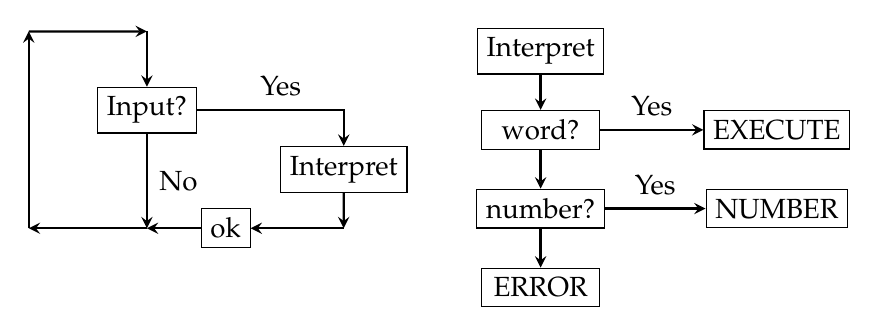
\begin{tikzpicture}[node distance=2cm]
            %Create nodes for left loop
            \node (input_1)     [wordinr1] {Input?}    ;
            \node (interpret_1) [wordinr1, right of = input_1, xshift=0.5cm, yshift=-0.75cm] {Interpret};
            \node (ok)          [wordinr1, below of = input_1, xshift=1.0cm, yshift=0.5cm] {ok};
            \coordinate[below of=input_1, yshift=0.5cm] (cont_1);
            \coordinate[left  of=cont_1,  xshift=0.5cm] (cont_2);
            \coordinate[above of=cont_2, yshift=0.5cm] (cont_3);
            \coordinate[above of=input_1, yshift=-1.0cm] (cont_4);
            \coordinate[below of=input_1, xshift=2.5cm, yshift=0.5cm] (cont_5);
            %Connect left loop
            \draw [arrow] (input_1.south) -- node[xshift=0.40cm] {No} (cont_1.north);
            \draw [arrow] (ok.west)       -- (cont_1.east);
            \draw [arrow] (cont_1.west)   -- (cont_2.east);
            \draw [arrow] (cont_2.north)  -- (cont_3.south);
            \draw [arrow] (cont_3.east)   -- (cont_4.west);
            \draw [arrow] (cont_4.south)  -- (input_1.north);
            %Connect right loop
            \draw [arrow] (input_1.east)  -| node[yshift=0.30cm, xshift=-0.80cm] {Yes} (interpret_1.north) ;
            \draw [arrow] (interpret_1.south) -- (cont_5.north);
            \draw [arrow] (cont_5.west) -- (ok.east) ;
            
            \node (interpret_2) [wordinr2, yshift=0.75cm, xshift=5.0cm]           {Interpret} ;
            \node (word)        [wordinr2, yshift=1.0cm,  below of = interpret_2] {word?}     ;
            \node (number_1)    [wordinr2, yshift=1.0cm,  below of = word, ]      {number?}   ;
            \node (error)       [wordinr2, yshift=1.0cm,  below of = number_1]    {ERROR}     ;
            \node (execute)     [wordinr2, xshift=1.0cm,  right of = word]        {EXECUTE}   ;
            \node (number_2)    [wordinr2, xshift=1.0cm,  right of = number_1]    {NUMBER}    ;
            \draw [arrow] (interpret_2) -- (word);
            \draw [arrow] (word)        -- (number_1);
            \draw [arrow] (number_1)    -- (error);
            \draw [arrow] (word)        -- node[yshift=0.30cm] {Yes} (execute);
            \draw [arrow] (number_1)    -- node[yshift=0.30cm] {Yes} (number_2);
        \end{tikzpicture}
    }
  \caption{\textit{Overview of FORTH outer interpreter}}
  \label{fig:Outer_interpreter}
\end{figure}

In general, because FORTH is interpretive as well as compiled, the best way to study something new is in front of a computer running FORTH. Therefore we explain with illustrations, expecting the reader to try them out.

In what follows, anything the user types in will be set in \lstinline$Helvetica$, such as \regc{DECIMAL} below.

Machine responses appear in ordinary type.

We now give a trivial illustration:

\begin{lstlisting}
DECIMAL <cr> ok
\end{lstlisting}

\underline{\textbf{Notes}}:
\begin{itemize}
  \item \bc{<cr>} means "the user pushes the ENTER or $\Leftarrow$ button".
  \item \bc{ok} is what FORTH says in response to an input line, if nothing has gone wrong.
  \item \regc{DECIMAL} is an instruction to use base 10 arithmetic. FORTH will use any base on tell it, within reason, but usually only \regc{DECIMAL} and \regc{HEX} (hexadecimal) are predefined.
\end{itemize}

When the outer interpreter (see fig. 2.1 on p. 13) encounters text with no dictionary entry, it tries to interpret it as a \bc{NUMBER}.

It places the number in a special memory location called "the top of the stack" (TOS)\footnote{We will explain about the stack in §2.3.}
\begin{lstlisting}
2 17 +. <cr> 19 ok
\end{lstlisting}

\underline{\textbf{Notes}}:
\begin{itemize}
  \item FORTH interprets 2 and 17 as numbers, and pushes them onto the stack. "\bc{+}" is a word and so is "\bc{.}" so they are \bc{EXECUTE}d.
  \item \lstinline$+$ adds 2 to 17 and leaves 19 on the stack.
  \item The word \bc{.} (called "emit") removes 19 from the stack and displays it on the screen.
\end{itemize}

We might also have said \footnote{since FORTH uses words, when we enter an input line we say the corresponding phrase.}

\begin{lstlisting}
HEX 0A 14 * . <cr> C8 ok
\end{lstlisting}

(Do you understand this? Hint: \bc{HEX} stands for "switch to hexadecimal arithmetic")

If the incoming text can neither be located in the dictionary nor interpreted as a number, FORTH issues an error message.


\section{Extending the dictionary}

\TallC{T}{he} compiler is one of FORTl-I’s most endearing features. It is elegant, simple, and mostly written in FORTH. Although the technical details of the FORTH compiler are generally more interesting to systems developers than to scientists, its components can often be used to solve programming problems. When this is the case, we necessarily discuss details of the compiler. In this section we discuss how the compiler extends the dictionary. In §2§§8 below we examine the parts of the compiler in greater detail.

FORTH has special words that allow the creation of new dictionary entries, \textit{i.e.}, new words. The most important are "\bc{:}" ("start a new definition") and "\bc{;}" ("end the new definition").

Consider the phrase

\begin{lstlisting}
: NEW-WORD WORD1 17 WORDZ . . . WORDn ; ok
\end{lstlisting}

The initial "\bc{:}" is \bc{EXECUTE}d because it is already in the dictionary. Upon execution, "\bc{:}" does the following:

\begin{itemize}
    \item Creates a new dictionary entry, \bc{NEW-WORD}, and switches from \textbf{interpret}- to \textbf{compile} mode.
    \item In compile mode, the interpreter looks up words and — rather than executin them — installs ointers to their code. If the text is a number (\bc{17} above), FORTH builds the literal number into the dictionary space allotted for \bc{NEW-WORD}.
    \item The action of \bc{NEW-WORD} will be to \bc{EXECUTE} sequentially the previously-defined words \bc{WORD1}, \bc{WORD2}, ...\bc{WORDn}, placing any built-in numbers on the stack as they occur.
    \item The FORTH compiler \bc{EXECUTE}s the last word "\bc{;}" of the definition, by installing code (to return control to the next outer level of the interpreter\footnote{This level could be either the outer interpreter or a word that invokes \bc{NEW-WORD}.}) then switching back from compile to interpret mode. Most other languages treat tokens like "\bc{;}" as flags (in the input stream) that \textit{trigger} actions, rather than actions in their own right FORTH lets components execute themselves.
\end{itemize}

In FORTH \textit{all} subroutines are words that are invoked when they are named. No explicit CALL or GOSUB statement is required.

The above definition of \textbf{NEW-WORD} is extremely structured compared with FORTRAN or BASIC. Its definition is just a series of subroutine calls.

\TallC{W}{e} now illustrate how to define and use a new word using the previously defined words "\bc{:}"and "\bc{;}". Enter the phrase (this new word \bc{*+} expects 3 numbers, \textit{a}, \textit{b}, and \textit{c} on the stack)

\begin{lstlisting}
: *+   * + ; ok
\end{lstlisting}

\underline{Notes:}
\begin{itemize}
    \item \bc{*} multiplies b with c, leaving b*c.
    \item \bc{+} then adds b*c to a, leaving a + b*c behind.
\end{itemize}

Now we actually try out \bc{*+} :

\begin{lstlisting}
DECIMAL 5 6 7 *+ . 47 ok
\end{lstlisting}

\underline{\textbf{Notes:}}
\begin{itemize}
    \item The period \bc{.} is not a typo, it EMlTs the result.
    \item FORTH's response to \bc{a b c *+ .} is \bc{a + b*c ok}.
\end{itemize}

What if we were to enter *+ with nothing on the stack? Let's try it and see (\bc{.S} is a word that displays the stack without changing its contents):

\begin{lstlisting}
.S empty stack ok

*+ empty stack ok
\end{lstlisting}

\dotrule{1\textwidth}

\underline{\textbf{Exercise:}}

Suppose you entered the input line

\begin{lstlisting}
HEX 5 6 7 *+ . <cr> xxx ok
\end{lstlisting}

What would you expect the response \textbf{xxx} to be?

\textit{Answer:} \bc{2F}

\dotrule{1\textwidth}

\section{Stacks and reverse Polish notation (RPN)}

\TallC{W}{e} now discuss the stack and the "reverse Polish" or "postfix" arithmetic based on it. (Anyone who has used one of the Hewlett-Packard calculators should already be familiar with the basic concepts.)

A Polish mathematician (J .Lukasewcleia) showed that numerical calculations require an irreducible minimum of elementary operations (fetching and storing numbers as well as addition, subtraction, multiplication and division). The minimum is obtained when the calculation is organized by "stack" arithmetic.

Thus virtually all central processors (CPU's) intended for arithmetic operations are designed around stacks. FORTH makes efficient use of CPU's by reflecting this underlying stack architecture in its syntax, rather than translating algebraic-looking program statements ("infix" notation) into RPN-based machine operations as FORTRAN, BASIC, C and Pascal do.

But what \textit{is} a stack? As the name implies, a stack is the machine analog of a pile of cards with numbers written on them. Numbers are always added to, and removed from, the top of the pile. (That is, a stack resembles a job where layoffs follow seniority: last in, first out.) Thus, the FORTH input line

\begin{lstlisting}
DECIMAL 2 5 73 -16 ok
\end{lstlisting}

followed by the line

\begin{lstlisting}
+ - * . yyy ok
\end{lstlisting}

leaves the stack in the successive states shown in Table 2-1 below

\begin{center}
    \begin{tabular}{|c c c c c c c|}
        \hline
   Cell\# & Initial    & Ops$\rightarrow$ & +       & -          & *       & . \\ [0.5ex] 
        \hline
        0 & \lgray -16 & Result        & \Aggray 57 & \dgray -52 & \gray 104 & ... \\ 
        1 & \lgray 73  & $\rightarrow$ & \Aggray 5  & \dgray 2   & ...       & ... \\
        2 & \lgray 5   &               & \Aggray 2  & ...        & ...       & ... \\
        3 & \lgray 2   &               & ...        & ...        & ...       & ... \\
        \hline
    \end{tabular}
\end{center}

Table 2-1 \textit{Picture of the stack during operations}

We usually employ zero-based relative numbering in FORTH data structures —stacks, arrays, tables, \textit{etc}.— so TOS ("top of stack") is given relative \#0, NOS ("next on stack") \#1, \textit{\textit{etc}}.

The operation "\bc{.}" ("emit") displays -104 to the screen, leaving the stack empty. That is, \bc{yyy} above is \bc{-104}.

\subsection{Manipulating the parameter stack}

\TallC{F}{ORTH} system incorporate (at least) two stacks: the \textbf{parameter} stack which we now discuss, and the \textbf{return stack} which we defer to 2.3.2.

In order to use a stack-based system, we must be able to put numbers on the stack, remove them, and rearrange their order. FORTH includes standard words for this purpose.

Putting numbers on the stack is easy: one simply types the number (or it appears in the definition of a FORTH word).

To remove a number we have the word \bc{DROP} that drops the number from TOS and moves up all the other numbers.

Tb exchange the top 2 numbers we have .

\bc{DUP} duplicates the TOS into NOS, pushing down all the other numbers.

\bc{ROT} rotates the top 3 numbers.

\begin{center}
    \begin{tabular}{|c c c c c c c|}
        \hline
   Cell\# & Initial    & Ops$\rightarrow$ & DROP   & SWAP        & ROT       & DUP\\ [0.5ex] 
        \hline
        0 & \lgray -16 & Result        & \Aggray 73 & \dgray 73  & \gray 5   & \digray -16 \\ 
        1 & \lgray 73  & $\rightarrow$ & \Aggray 5  & \dgray -16 & \gray -16 & \digray -16 \\
        2 & \lgray 5   &               & \Aggray 2  & \dgray 5   & \gray 73  & \digray 73  \\
        3 & \lgray 2   &               & ...        & \dgray 2   & \gray 2   & \digray 5   \\
        4 & \lgray ... &               & ...        & ...        & ...       & \digray 2   \\
        \hline
    \end{tabular}
\end{center}

Table 2-2 \textit{Stack manipulation operators}

These actions are shown on page 19 above in Thble 2—2 (we show what each word does to the initial stack).

In addition the words \bc{OVER}, \bc{UNDER}, \bc{PICK} and \bc{ROLL} act as shown in Table 2-3 below (note \bc{PICK} and \bc{ROLL} must be preceded by an integer that says where on the stack an element gets  \bc{PICK}ed or \bc{ROLL}ed).

\begin{center}
    \begin{tabular}{|c c c c c c c|}
        \hline
   Cell\# & Initial    & Ops$\rightarrow$ & OVER   & UNDER        & 4 PICK  & 4 ROLL \\ [0.5ex] 
        \hline
        0 & \lgray -16 & Result        & \Aggray 73  & \dgray -16 & \gray 2   & \digray 2   \\ 
        1 & \lgray 73  & $\rightarrow$ & \Aggray -16 & \dgray 73  & \gray -16 & \digray -16 \\
        2 & \lgray 5   &               & \Aggray 73  & \dgray -16 & \gray 73  & \digray 73  \\
        3 & \lgray 2   &               & \Aggray 5   & \dgray 5   & \gray 5   & \digray 5   \\
        4 & \lgray ... &               & \Aggray 2   & \dgray 2   & \gray 2   & ...         \\
        \hline
    \end{tabular}
\end{center}

Table 2-3 \textit{More stack manipulation operators}

Clearly, \bc{1 PICK} is the same as \bc{DUP}, \bc{2 PICK} is a synonym for \bc{OVER}, \bc{2 ROLL} means \bc{SWAP}, and \bc{3 ROLL} means \bc{ROT}.

As Brodie has noted (\TF), it is rarely advisable to have aword use a stack so deep that \bc{PICK} or \bc{ROLL} is needed. It is generally better to keep word definitions short, using only a small number of arguments on the stack and consuming them to the extent possible. On the other hand, \bc{ROT} and its opposite, \bc{-ROT}\footnote{defined as \bc{: -ROT ROT ROT ;}}, are often useful.

\subsection{The return stack and Its uses}
\TallC{W}{e} have remarked above in §2§§2 that compilation establishes links from the calling word to the previously- defined word being invoked. Part of the linkage mechanism ——during actual execution- is the \textbf{return stack} (rstack): the address of the next word to be invoked after the currently executing word is placed on the rstack, so that when the current word is done, the system jumps to the next word. Although it might seem logical to call the address on the rstack the \textbf{next} address, it is actually called the \textbf{return} address for historical reasons.

In addition to serving as a reservoir of return addresses (since words can be nested, the return addresses need a stack to be put on) the rstack is where the limits of a \bc{DO ... LOOP} construct are placed\footnote{We discuss looping in 2.7 below.}

The user can also store/retrieve to/from the rstack This is an example of using a component for a purpose other than the one it was designed for. Such use is not encouraged by every FORTH text, needless to say, since it introduces the spice of danger. To store to the rstack we say \bc{>R}, and to retrieve we say \bc{R>}. \bc{DUP>R} is a speedup of the phrase \bc{DUP >R}. The words \bc{D>R DR>} , for maving double-length integers, also exist on many systems. The word \bc{R@} copies the top of the rstack to the TOS.

\leftbar[1\linewidth]
\textbf{The danger is this:} anything put on the rstack during a word’s execution must be removed before the word terminates. If the \bc{>R} and the \bc{R>} do not balance, then a \textbf{wrong next address} will be jumped to and \bc{EXECUTE}d. Since this could be the address of data, and since it is being interpreted as machine instructions, the results will be \textbf{always unpredictable}, but seldom amusing.
\endleftbar

Why would we want to use the rstack for storage when we have a perfectly good parameter stack to play with? Sometimes it becomes simply impossible to read code that performs complex gymnastics on the parameter stack, even though FORTH permits such gymnastics.

Consider a problem — say, drawing a line on a bit- mapped graphics output device from (x,y) to (x',y')— that requires 4 arguments. We have to turn on the appropriate pixels in the memory area representing the display, in the ranges from the origin to the end coordinates of the line. Suppose we want to work with x and y first, but they are 3rd and 4th on the stack. So we have to \bc{ROLL} or \bc{PICK} to get them to TOS where they can be worked with conveniently. We probably need them again, so we use

\begin{lstlisting}
4PICK 4PICK ( -- x y x' y' x y)
\end{lstlisting}

Now 6 arguments are on the stack! See what I mean? A better way stores temporarily the arguments x’ and y', leaving only 2 on the stack. If we need to duplicate them, we can do it with an already existing word, \bc{DDUP}.

Complex stack manipulations can be avoided by defining \bc{VARIABLE}s —named locations— to store numbers. Since FORTH, variables are typically \textit{global} —any word can access them — their use can lead to unfortunate and unexpected interactions among parts of a large program. Variables should be used sparingly.

While FORTH permits us to make variables local to the sub- if routines that use them\footnote{See \FTR, p. 3253 for a description of beheading - a process to make variables local to a small set of subroutines. Another technique is to embed variables within a data structure so they cannot be referenccd inadvertently. Chapters 2§8§§3-2, 3§5§§2, 5§1§§2 and 11§2 offer examples.}, for many purposes the rstack can advantageously replace local variables:

\begin{itemize}
    \item The rstack already exists, so it need not be defined anew.
    \item When the numbers placed on it are removed, the rstack shrinks, thereby reclaiming some memory.
\end{itemize}

Suppose, in the previous example, we had put x’ and y’ on the rstack via the phrase

\begin{lstlisting}
    >R >R DDUP .
\end{lstlisting}

Then we could duplicate and access x and y with no trouble.

\leftbar[1\linewidth]
\underline{\textbf{A note of caution}}: since the rstack is a critical component of the execution mechanism, we mess with it at our peril. If we want to use it, we must clean up when we are done, so it is in the same state as when we found it. A word that places a number on the rstack must get it off again — using \bc{R>} or \bc{RDROP} — before exiting that word\footnote{\textbf{RDROP} is a handy way to exit from a word before reaching the final ";". See \TF.}. Similarly, since no LOOP uses the rstack also, for each >R in such a loop (after DO) there must be a corresponding R > or RDROP (before LOOP is reached). Otherwise the results will be unpredictable and probably will crash the system.
\endleftbar

\section{Fetching and storing}

\TallC{O}{rdinary} (16-bit) numbers are f\textit{etc}hed from memory to the stack by "\bc{@}" ("fetch"), and stored by "\bc{!}" ("store"). The word @ expects an address on the stack and replaces that address by its contents using, \textit{e.g.}, the phrase \bc{X @}. The word "\regc{!}" expects a number (NOS) and an address (T OS) to store it in, and places the number in the memory location referred to by the address, consuming both arguments in the process, as in the phrase \bc{32 X !}

Double length (32-bit) numbers can similarly be f\textit{etc}hed and stored, by \bc{D@} and \bc{DI} . (FORTH systems designed for the newer 32-bit machines sometimes use a 32-bit-wide stack and may not distinguish between single- and double-length integers.)

Positive numbers smaller than 255 can be placed in single bytes of memory using \bc{C@} and \bc{C!}. This is convenient for operations with strings of ASCII text, for example screen, file and keyboard I/O.

In Chapters 3, 4, S and 7 we shall extend the lexicon of \regc{@} and \regc{!} words to include floating point and complex numbers.

\section{Arlthmetlc operations}

\TallC{T}{he} 1979 or 1983 standards, not to mention the forthcoming ANSII standard, require that a conforming FORTH system contain a certain minimum set of predefined words. These consist of arithmetic operators \bc{+ — * / MOD /MOD */} for (usually) 16-bit \textit{signed-integer} (-32767 to +32767) arithmetic, and equivalents for \textit{unsigned} (0 to 65535), double-length and mixed-mode (16- mixed with 32-bit) arithmetic. The list will be found in the glossary accompanying your system, as well as in \SF and \FTR.

\section{Comparing and testlng}

TallC{I}{n} addition to arithmetic, FORTH lets us compare numbers on the stack, using relational operators \bc{> < =}.These operators work as follows: the phrase

\begin{lstlisting}
    2 3 > < cr > ok
\end{lstlisting}

will leave 0 ("false") on the stack, because 2 (N0S) is not greater
than 3 (TOS). Conversely, the phrase

\begin{lstlisting}
    23 < <cr> ok
\end{lstlisting}

will leave -1 ("true") because 2 is less than 3. Relational operators typically consume their arguments and leave a "flag" to show what happened\footnote{The original FORTH-79 used +1 for "true", 0 for "false"; many newer system that mostly follow FORTH-79 use -1 for "true". HS/FORTH is one such. Both FORTH-83 and ANSII FORTH require -1 for "true", 0 for "false".}. Those listed so far work with signed 16-bit integers. The operator \bc{U<} tests \textit{unsigned} 16-bit integers (0-65535).

FORTH offers unary relational operators \bc{0= 0>} and \bc{0<} that determine whether the TOS contains a (signed) 16-bit integer that is 0, positive or negative. Most FORTHs offer equivalent relational operators for use with double-length integers.

The relational words are used for branching and control. The usual form is

\begin{lstlisting}
    : MAYBE 0> IF WORDl WORD2 ...
      WORDn THEN ;
\end{lstlisting}

The word \bc{MAYBE} expects a number on the stack, and executes the words between \bc{IF} and \bc{THEN} if the number on the stack is positive, but not otherwise. If the number initially on the stack were negative or zero, \bc{MAYBE} would do nothing.

An alternate form including \bc{ELSE} allows two mutually exclusive actions:

\begin{lstlisting}
    : CHOOSE 0> IF WORD1 . . . WORDn
            ELSE WORDt' . . . WORDn'
            THEN ; (n -- )
\end{lstlisting}

If the number on the stack is positive, \bc{CHOOSE} executes \bc{WORD1 WORD2... WORD}, whereas if the number is negative or 0, \bc{CHOOSE} executes \bc{WORD1'} ... \bc{WORDn'}.

In either example, \bc{THEN} marks the end of the branch, rather than having its usual logical meaning\footnote{This has led some FORTH gurus to prefer the synonymous word \bc{ENDIF} as clearer than \bc{THEN}.}.

\section{Looping and structured programming}

\TallC{F}{ORTH} contains words for setting up loops that can be definite or indefinite:

\begin{lstlisting}
    BEGIN xxx flag UNTIL
\end{lstlisting}

The words represented by \bc{xxx} are executed, leaving the TOS (flag) set to 0 (F) -at which point \bc{UNTIL} leaves the loop - or -1 (T) -at which point \bc{UNTIL} makes the loop repeat from \bc{BEGIN}.

A variant is
\begin{lstlisting}
    BEGIN xxx flag WHILE yyy REPEAT
\end{lstlisting}

Here \bc{xxx} is executed, \bc{WHILE} tests the flag and if it is 0 (F) leaves the loop; whereas if flag is -1 (T) \bc{WHILE} executes \bc{yyy} and \bc{REPEAT} then branches back to \bc{BEGIN}. These forms can be used to set up loops that repeat until some external event (pressing a key at the keyboard, \textit{e.g.}) sets the flag to exit the loop. They can also used to make endless loops (like the outer interpreter of FORTH) by forcing flag to be 0 in a definition like

\begin{lstlisting}
    : ENDLESS BEGIN xxx 0 UNTIL ;
\end{lstlisting}

\TallC{F}{ORTH} also implements indexed loops using the words \bc{DO LOOP +LOOP /LOOP}. These appear within definitions, \textit{e.g.}

\begin{lstlisting}
    : LOOP-EXAMPLE 100 0 DO xxx LOOP ;
\end{lstlisting}

The words \bc{xxx} will be executed 100 times as the lower limit, 0, increases in unit steps to 99. To step by -2's, we use the phrase

\begin{lstlisting}
    -2 + LOOP
\end{lstlisting}

to replace \bc{LOOP}, as in

\begin{lstlisting}
    : DOWN-BY-2's O 100 DO xxx -2 +LOOP ;
\end{lstlisting}

The word \bc{/LOOP} 1s a variant of \bc{+LOOP} for working with unsigned limits\footnote{Signed 16-bit integers run from -32768 to +32767, unsigned from 0 to 65535. See \FTR.} and increments (to permit the loop index to go up to 65535 in 16-bit systems).

\section{The pearl of FORTH}

An unusual construct, \bc{CREATE...DOES>}, has been called "the pearl of FORTH" \footnote{Michael Ham, "Structured Programming", \textit{Dr. Dobb's Journal of Software Tools}, October, 1986.} This is more than poetic license.

\bc{CREATE} is a component of the compiler that makes a new dictionary entry with a given name (the next name in the input stream) and has no other function.

\bc{DOES>} assigns a specific run-time action to a newly \bc{CREATE}d word (we shall see this in §2§§8-3 below).

\subsection{Dummy words}
Sometimes we use \bc{CREATE} to make a dummy entry that we can later assign to some action:
\begin{lstlisting}
    CREATE DUMMY
    CA' * DefinES DUMMY
\end{lstlisting}

The second line translates as "The code address of \bc{*} defines \bc{DUMMY}". Entry of the above phrase would let \bc{DUMMY} perform the job of \bc{*} just by saying \bc{DUMMY}. That is, FORTH lets us first define a dummy word, and then give it any other word’s meaning \footnote{This usage is a non-standard construct of HS/FORTH.}.

Here is one use of this power: Suppose we have to define two words that are alike except for some piece in the middle:
\begin{lstlisting}
    : *WORD  WORD1 WORD2 *  WORD3 WORD4 ;
    : */WORD WORD1 WORD2 */ WORD3 WORD4 ;
\end{lstlisting}

we could get away with 1 word, together with \bc{DUMMY} fromabove,

\begin{lstlisting}
    : *_or_*/WORD
        WORD1 WORD2
        DUMMY
        WORD3 WORD4 ;
\end{lstlisting}
by saying
\begin{lstlisting}
    CA' * DefinES DUMMY *_or_*/WORD
\end{lstlisting}
or
\begin{lstlisting}
    CA' */ DefinES DUMMY *_or_*/WORD
\end{lstlisting}

This technique, a rudimentary example of vectoring, saves memory and saves programming time by letting us vary something in the middle of a definition \textit{after the definition has been entered in the dictionary}. However, this technique must be used with caution as it is akin to \textbf{self-modifying} code\footnote{Self-modifying machine code is considered a serious "no-no" by modern structured programming standards. Although it is sometimes valuable, few modern cpu's are capable of handling it safely. More often, because cpu's tend to use pipelining and parallelism to achieve speed, a piece of code might be modified in memory, but - having been pre-fetched before modification - actually execute in unmodified form.}

A similar procedure lets a subroutine call itself recursively, an enormous help in coding certain algorithms.

\subsection{Defining "defining" words}

\TallC{T}{he} title of this section is neither a typo nor a stutter: \bc{CREATE} finds its most important use in extending the powerful class of FORTH words called "defining" words. The colon compiler "\bc{:}" is such a word, as are \bc{VARIABLE} and \bc{CONSTANT}. The definition of \bc{VARIABLE} is simple

\begin{lstlisting}
    : VARIABLE CREATE 2 ALLOT ;
\end{lstlisting}

Here is how we use it:
\begin{lstlisting}
    VARIABLE X <cr> ok
\end{lstlisting}

The inner workings of VARIABLE are these:
\begin{itemize}
    \item \bc{CREATE} makes a dictionary entry with the next name in the input stream — in this case, \bc{X}.
    \item Then the number 2 is placed on the stack, and the word \bc{ALLOT} increments the pointer that represents the current location in the dictionary by 2 bytes.
    \item This leaves a 2-byte vacancy to store the value of the variable (that is, the next dictionary header begins 2 bytes above the end of the one just defined).
\end{itemize}

When the outer interpreter loop encounters a new \bc{VARIABLE}'s name in the input stream, that name’s address is placed on the stack. But this is also the location where the 2 bytes of storage begins. Hence when we type in \bc{X}, the TOS will contain the storage address named \bc{X}.

As noted in §2.4 above, the phrase \bc{X @} (pronounced "X f\textit{etc}h") places the contents of address \bc{X} on the stack, dropping the address in the process. Conversely, to store a value in the named location \bc{X}, we use \bc{!} ("store"): thus
\begin{lstlisting}
    4 X ! <cr> ok
    X @ . <cr> 4 ok
\end{lstlisting}

Double-length variables are defined \textit{via} \bc{DVARIABLE}, whose definition is

\begin{lstlisting}
    : DVARIABLE CREATE 4 ALLOT ;
\end{lstlisting}

\TallC{F}{ORTH} has a method for defining words initialized to contain specific values: for example, we might want to define the number 17 to be a word. \bc{CREATE} and "\bc{,}" ("comma") let us do this as follows:

\begin{lstlisting}
    17 CREATE SEVENTEEN , <cr> ok
\end{lstlisting}

Now test it \textit{via}

\begin{lstlisting}
    SEVENTEEN @ . <cr> 17 ok
\end{lstlisting}

\underline{\textbf{Note}}: The word "," ("comma") puts TOS into the next 2 bytes of the dictionary and increments the dictionary pointer by 2.

A word \bc{C}, ("see-comma") puts a byte-value into the next byte of the dictionary and increments the pointer by 1 byte.

\subsection{Run-time vs. compile-time actions}

\TallC{I}{n} the preceding example, we were able to initialize the variable \bc{SEVENTEEN} to 17 when we \bc{CREATE}d it, but we still have to fetch it to the stack \textit{via} \bc{SEVENTEEN @} whenever we want it. This is not quite what we had in mind: we would like to find 17 in T0S when we say \bc{SEVENTEEN}. The word \bc{DOES>} gives us precisely the tool to do this.

As noted above, the function of \bc{DOES>} is to specify a run-time action for the "child" words of a defining word. Consider the defining word \bc{CONSTANT}, defined in high-level\footnote{Of course \bc{CONSTANT} is usually a machine—code primitive, for speed.} FORTH by

\begin{lstlisting}
    : CONSTANT CREATE , DOES> @ ;
\end{lstlisting}
and used as
\begin{lstlisting}
    53 CONSTANT PRIME ok
\end{lstlisting}

Now test it:
\begin{lstlisting}
    \textbf{PRIME} . <cr> 53 ok
\end{lstlisting}

What happened?
\begin{itemize}
    \item \bc{CREATE} (hidden in \bc{CONSTANT}) made an entry (named \bc{PRIME} , the first word in the input stream following \bc{CONSTANT}). Then "\bc{,}" placed the TOS (the number 53) in the next two bytes of the dictionary.
    \item \bc{DOES>} (inside \bc{CONSTANT}) then appended the actions of all words between it and "\bc{;}" (the end of the definition of \bc{CONSTANT}) to the child word(s) defined by \bc{CONSTANT}.
    \item In this case, the only word between \bc{DOES>} and \bc{;} was \bc{@} , so all FORTH constants defined by CONSTANT perform the action of placing their address on the stack (anything made by \bc{CREATE} does this) and fetching the contents of this address.
\end{itemize}

\subsubsection{Klingons}

\TallC{L}{et} us make a more complex example. Suppose we had previously defined a word \bc{BOX ( n x y -- )} that draws a small square box of n pixels to a side centered at (x, y) on the graphics display. We could use this to indicate the instantaneous location of a moving object -- say a Klingon space-ship in a space-war game.

So we define a defining word that creates (not very realistic looking) space ships as squares n pixels on a side:

\begin{lstlisting}
    : SPACE-SHIP CREATE , DOES>
        @-ROT (--nxy)      BOX ;
    : SIZE ; \ do-nothing word
\end{lstlisting}

Now, the usage would be (\bc{SIZE} is included merely as a reminder of what 5 means -- it has no function other than to make the definition look like an English phrase)

\begin{lstlisting}
    SIZE 5 SPACE-SHIP KLINGON <cr> ok
    71 35 KLINGON <cr> ok
\end{lstlisting}

Of course, \bc{SPACE-SHIP} is a poorly constructed defining word because it does not do what it is intended to do. Its child-word \bc{KLINGON} simply draws itself at (x, y).

What we really want is for \bc{KLINGON} to \textit{undraw} itself from its old location, compute its new position according to a set of rules, and then redraw itself at its new position This sequence of operations would require a definition more like

\begin{lstlisting}
    :OLD.POS@ (adr--adr n x y) DUP @ OVER
      2+ D@ :
    : SPACE-SHIP CREATE , 4 ALLOT DOES>
       OLD.POS@ UNBOX NEW.POSI
       OLD.POS@ BOX DROP ;
\end{lstlisting}

where the needed specialized operation \bc{UNBOX} would be defined previously along with \bc{BOX}.

\subsubsection{Dimensioned data (with Intrinsic unlts)}
Here is another example of the power of defining words and of the distinction between compile-time and run-time behaviors.

Physical problems generally work with quantities that have dimensions, usually expressed as mass (M), length (L) and time (T) or products of powers of these. Sometimes there is more than one system of units in common use to describe the same phenomena.

For example, traffic police reporting accidents in the United States or the United Kingdom might use inches, feet, and yards; whereas Continental police would use the metric system. Rather than write different versions of an accident analysis program it is simpler to write one program and make unit conversions part of the grammar. This is easy in FORTH; impossible in FORTRAN, BASIC, Pascal, or C; and possible, but exceedingly cumbersomein Ada\footnote{An example (and its justification) of dimensioned data types in Ada is given by Do-While Jones, \textit{Dr. Dobb's Journal}, March 1987. The FORTH solution below is much simpler than the Ada version.}.

We simply keep all internal lengths in millimeters, say, and con-
vert as follows\footnote{This example is based on 16-bit integer arithmetic. The word \regc{*/} means "multiply the third number on the stack by NOS, keeping 32 bits of precision, and divide by "TOS". That is, the stack comment for \regc{*/} is \regc{(a b c --a*b/c)}.}:

\begin{lstlisting}
    : INCHES  254 10 */ ;
    : FEET  [ 254 12 * ] LITERAL 10 */ ;
    : YARDS [ 254 36 * ] LITERAL 10 */ ;
    : CENTIMETERS 10 * ;
    : METERS 1000 * ;
\end{lstlisting}

The usage would be
\begin{lstlisting}
    10 FEET . <cr> 3048 ok
\end{lstlisting}

These are more definitions than necessary, of course, and the technique generates unnecessary code. A more compact approach uses a \textit{defining word}, \bc{UNITS}:

\begin{lstlisting}
    : D, SWAP , , ; \ I double—length # in next cells
    : UNITS CREATE D, DOES> D@ */ ;
\end{lstlisting}

Then we could make the table
\begin{lstlisting}
    254  10         UNITS INCHES
    254  12 * 10    UNITS FEET
    254  36 * 10    UNITS YARDS
     10   1         UNITS CENTIMETERS
    1000  1         UNITS METERS
    \ Usage:
    \ 10 FEET . <cr> 3048 ok
    \ 3  METERS . <cr> 3000 ok
    \ ......
    \ \textit{etc}.
\end{lstlisting}

This is an improvement, but FORTH lets us do even better: here is a simple extension that allows conversion back to the input units, for use in output:

\begin{lstlisting}
    VARIABLE <AS>                \ new variable
    0 <AS> !                     \ initialize to "F"
    : AS -1 <AS> ! ;             \ set <AS> = "T"
    : UNITS CREATE D, DOES>
       D@                        \ get 2 #s
       <AS> @                    \ get current val.
          IF SWAP THEN           \ flip if "true"
      */   0 <AS> ! ;            \ convert, reset <AS>

    BEHEAD' <AS>          \ make it local for security(*@\footnote{Headerless words are described in \FTR, p. 325ff. The word \textbf{BEHEAD'} is HS/FORTH's method for making a normal word into a headerless one. See Ch. 5\S1\S\S3 for further details.} @*)
    \ unit definitions remain the same
    \ Usage:
    \ 10 FEET      . <cr> 3048 ok
    \ 3048 AS FEET . <cr> 10 ok
\end{lstlisting}

\subsection{Advanced methods of controlllng the compiler}

\TallC{F}){ORTH} includes a technique for switching from compile mode to interpret mode while compiling or interpreting. This is done using the words \bc{]} and \bc{[} . (Contrary to intuition, \bc{]} turns the compiler on, \bc{[} turns it off.)

One use of \bc{]} and \bc{[} is to create an "action table" that allows us to choose which of several actions we would like to perform\footnote{Better methods will be described in Chapter 5.}.

For example, suppose we have a series of push-buttons numbered 1-6, and a word \bc{WHAT} to read them.

That is, \bc{WHAT} waits for input from a keypad; when button \#3 is pushed, \textit{e.g.}, \bc{WHAT} leaves 3 on the stack.

We would like to use the word \bc{BUTTON} in the following way:

\begin{lstlisting}
    WHAT BUTTON
\end{lstlisting}

\bc{BUTTON} can be defined to choose its action from a table of
actions called \bc{BUTTONS} . We define the words as follows:

\begin{lstlisting}
    CREATE BUTTONS ] RING-BELL OPEN-DOOR
      ENTER LAUGH CRY SELF-DESTRUCT [
    : BUTTON 1- 2* BUTTONS + @ EXECUTE ;
\end{lstlisting}

If, as before, I push \#3, then the action \bc{ENTER} will be executed. Presumably button \#7 is a good one to avoid\footnote{The safety of an execution table can be increased by making the first (that is, the zero’th) action \textbf{WARNING}, and making the first step of \bc{BUTTON} a word \bc{CHECK-DATA} that maps any number not in the range 1-6 into 0. Then a wrong button number causes a \textbf{WARNING} to be issued and the system resets.}.

How does this work?
\begin{itemize}
    \item \bc{CREATE BUTTONS} makes a dictionary entry \bc{BUTTONS}.
    \item \bc{]} turns on the compiler: the previously-defined word-names \bc{RING-BELL}, \textit{etc.} are looked up in the dictionary and compiled into the table (as though we had begun with :), rather than being executed.
    \item \bc{[} returns to interactive mode (as if it were ;), so that the next colon definition (\bc{BUTTON}) can be processed.
    \item The table \bc{BUTTONS} now contains the code-field addresses (CFA’s) of the desired actions of \bc{BUTTON}.
    \item \bc{BUTTON} first uses 1- to subtract 1 from the button number left on the stack by \bc{WHAT} (so we can use 0—based numbering into the table -- if the first button were \# 0, this would be unneeded).
    \item \bc{2*} then multiplies by 2 to get the offset (from the beginning of \bc{BUTTONS}) of the CFA representing the desired action.
    \item \bc{BUTTONS +} then adds the base address of \bc{BUTTONS} to get the absolute address where the desired CPA is stored.
    \item \bc{@} fetches the CFA for \bc{EXECUTE} to execute.
    \item \bc{EXECUTE} executes the word corresponding to the button pushed. Simple!
\end{itemize}

You may well ask "Why bother with all this indirection, pointers, pointers to pointers, tables of pointers to tables of pointers, and the like?" Why not just have nested \bc{IF...ELSE...THEN} constructs, as in Pascal?

There are three excellent reasons for using pointers:
\begin{itemize}
    \item Nested \bc{IF...THEN}'s uickly become cumbersome and difficult to decipher (\TF). They are also \underline{\textbf{slow}} (see Ch. 11).
    \item Changing pointers is generally much faster than changing other kinds of data -- for example reading in code overlays to accomplish a similar task.
    \item The unlimited depth of indirection possible in FORTH permits arbitrary levels of abstraction. This makes the computer behave more "intelligently" than might be possible with more restrictive languages.
\end{itemize}

A similar facility with pointers gives the C language its abstractive power, and is a major factor in its popularity.

\section{Strings}

\TallC{B}{y} now it should be apparent that FORTH can do anything any other language can do. One feature we need in any sort of programming --scientific or otherwise-- is the ability to handle alphanumeric strings. We frequently want to print messages to the console, or to put captions on figures, even if we have no interest in major text processing.

While every FORTH system must include words to handle strings(see, e.g., \FTR Ch. 9) --the very functioning of the outer interpreter, compiler, \textit{etc.}, demands this-- there is little unanimity in defining extensions. BASIC has particularly good string-handling features, so HS/FORTH and others provide extensions designed to mimic BASIC’s string functions.

Typical FORTH strings are Iimite to 255 characters because they contain a count in their first byte\footnote{A single byte can represent positive numbers 0-255.}.The word \bc{COUNT}
\begin{lstlisting}
    : COUNT DUP 1+ SWAP C@ ; (adf--nadr+1)
\end{lstlisting}

expects the address of a counted string, and places the count and
the address of the first character of the string on the stack. \bc{TYPE}, a required ’79 or ’83 word, prints the string to the console.

It is straightforward to employ words that are part of the system (such as \bc{KEY} and \bc{EXPECT}) to define a word like \bc{$"} that takes all characters typed at the keyboard up to a final \bc{"} (close-quote --not a word but a string-terminator), makes a counted string of them, and places the string in a buffer beginning at an address returned by \bc{PAD}\footnote{A system variable that returns the current starting address of the "scratchpad".}.

The word \bc{$.} ("string-emit") could then be defined as
\begin{lstlisting}
    : $. COUNT TYPE ; (adr --)
\end{lstlisting}

and would be used with 3" like this:
\begin{lstlisting}
    $' The quick brown fox" < cr> ok
    S. The quick brown fox ok
\end{lstlisting}

Since this book in not an attempt to paraphrase \FTR it is strongly recommended that the details of using the system words to devise a string lexicon be studied there.

\leftbar[1\linewidth]
One might contemplate modifying the \FTR lexicon by using a full 16-bit cell for the count. This would permit strings of up to 64k bytes (using unsigned integers\footnote{\FTR, Ch. 3.}), wasting 1 byte of memory per short ( 255 bytes) string. Although few scientific applications need to manipulate such long strings, the program that generated the index to this book needed to read a page at a time, and thus to handle strings about 3-5 kbytes long.
\endleftbar 

\section{FORTH programming style}

\TallC{A}{} FORTH program typically looks like this
\begin{lstlisting}
    \ Example of FORTH program
    :WORD1 ... ;
    :WORD2 OTHER-WORDS ;
    :WORDS YET-OTHER-WORDS ;
       ...
    : LAST-WORD wonon ...WORD3
       WORD2 WORD1 ;
    LAST-WORD <cr> \ run program
\end{lstlisting}

\leftbar[1\linewidth]
\textbf{\underline{Note}}: The word \ means "disregard the rest of this line". It is a convenient method for commenting code.
\endleftbar

In other words, a FORTH program consists of a series of word definitions, culminating in a definition that invokes the whole shebang. This aspect gives FORTH programming a somewhat different flavor from programming in more conventional languages.

Brodie notes in \TF that high-level programming languages are considered good if they require structured, top-down programming, and \textit{wonderful} if they impose \textit{information hiding}. Languages such as FORTRAN, BASIC and assembler that permit direct jumps and do not impose structure, top-down design and data-hiding are considered \textit{primitive} or bad. To what extent does FORTH follow the norms of good or \textit{wonderful} programming practice?

\subsection{Structure}

\TallC{T}{he} philosophy of "structured programming" entered the general consciousness in the early 1970’s. The idea was to make the logic of program control flow immediately apparent, thereby aiding to produce correct and maintainable programs. The language Pascal was invented to impose by fiat the discipline of structure. To this end, direct jumps (GOTOs) were omitted from the language\footnote{Ironially, most programmers refuse to get along without spaghetti code, so commercial Pascal's now include GOTO. Only FORTH among major languages completely eschews both line labels and GOTOs, making it the most structured language available.}.

FORTH programs are automatically structured because word definitions are nothing but subroutine calls. The language contains no direct jump statements (that is, no GOTO's) so it is \textit{impossible} to write "spaghetti" code.

A second aspect of structure that FORTH imposes (or at least encourages) is \textit{short} definitions. There is little speed penalty incurred in breaking a long procedure into many small ones, unlike more conventional languages. Each of the short words has one entry and one exit point, and does one job. This is the beaux ideal of structured programming!

subsection{"Top-down" design}

TallC{M}{ost} authors of "how to program" books recommend designing the entire program from the general to the particular. This is called "top-down" programming, and embodies these steps:

\begin{itemize}
    \item Make an outline, flow chart, data-flow diagram or whatever, taking a broad overview of the whole problem.
    \item Break the problem into small pieces (decompose it).
    \item Then code the individual components.
\end{itemize}

The natural programming mode in FORTH is "bottom-up" rather than "top-down" -- the most general word appears last, whereas the definitions necessarily progress from the primitive to the complex. It is possible -- and sometimes vital -- to invoke a word before it is defined ("forward referencing"\footnote{The FORmula TRANsIator in Ch. 11.4 uses this method to implement its recursive structure.} ). The dictionary and threaded compiler mechanisms make this nontrivial. The naturalness of bottom-up programming encourages a somewhat different approach from more familiar languages:

\begin{itemize}
    \item In FORTH, components are specified roughly, and then 3 they are coded they are immediately tested, debugged, redesigned and improved.
    \item The evolution of the components guides the evolution of the outer levels of the program.
\end{itemize}

We will observe this evolutionary style in later chapters as we design actual programs.

\subsection{Information hiding}

\TallC{I}{nformation} (or data) "hiding" is another doctrine of structured programming. It holds that no subroutine should have access to, or be able to alter (corrupt!) data that it does not absolutely require for its own functioning\footnote{Rather like the "cell" system in revolutionary conspiracies, where members of a cell know only each other but not the members of other cells. Mechanisms for receiving and transmitting messages between cells are double-blind. Hence, if an individual is captured or is a spy, he can betray at most his own cell and the damage is limited.}.

Data hiding is used both to prevent unforeseen interactions between pieces of a large program; and to ease designing and debugging a large program. The program is broken into small, manageable chunks ("black boxes") called \textbf{modules} or \textbf{objects} that communicate by sending messages to each other, but are otherwise mutually impenetrable. Information hiding and modularization are now considered so important that special languages --Ada, MODULA-Z, C++, and Object Pascal-- have been devised with it in mind.

To illustrate the problem information hiding is intended to solve, consider a FORTRAN program that calls a subroutine

\begin{lstlisting}
    PROGRAM MAIN
        some lines
    CALL SUB1(arg1, ar92, ... , argn, answer)
        some lines
    END

    SUB1(X1, ... , Xn, Y)
        some lines
        Y = something
    RETURN
    END
\end{lstlisting}

There are two ways to pass the arguments from MAIN to SUB1, and FORTRAN can use both methods.

\begin{itemize}
    \item Copy the arguments from where they are stored in MAIN into locations in the address space of SUBl (set aside for them during compilation). If the STATEMENTS change the values X1,...,Xn during execution of SUBl, the original values in the callin program will not be affected (because they are stored elsew ere and were copied during the CALL).
    \item Let SUBl have the addresses of the arguments where they are stored in MAIN. This method is dangerous because if the arguments are changed during execution of SUBl, they are changed in MAIN and are forever corrupted. If these changes were unintended, they can produce remarkable bugs.
\end{itemize}

Although copying arguments rather than addresses seems safer, sometimes this is impossible either because the increased memory overhead may be infeasible in problems with large amounts of data, or because the extra overhead of subroutine calls may unacceptably slow execution.

What has this to do with FORTH?

\begin{itemize}
    \item FORTH uses linked lists of addresses, compiled into a dictionary to which all words have equal right of access.
    \item Since everything in FORTH is a word --constants, variables, numerical operations, I/O procedures-- it might seem impossible to hide information in the sense described above.
    \item Fortunately, word-names can be erased from the dictionary after their CFAs have been compiled into words that call them. (This erasure is called "beheading".)
    \item Erasing the names of variables arantees they can be neither accessed nor corrupted by unauthorized words (except through a calamity so drea ful the program crashes).
\end{itemize}

\subsection{Documenting and commenting FORTH code}

\TallC{F}{ORTH} is sometimes accused of being a "write-only language. In other words, some complain that FORTH is cryptic. I feel this is basically a complaint against poor documentation and unhelpful word names, as Brodie and others have noted.

Unreadability is equally a flaw of poorly written FORTRAN, Pascal, C, \textit{et al}.

FORTH offers a programmer who takes the trouble a goodly array of tools for adequately documenting code.

\subsubsection{Parenthesized remarks}
The word ( --a left parenthesis followed by a space-- says "disregard all following text up until the next right parenthesis\footnote{The right parenthesis, ) , is not a word but a \textbf{delimiter}.} in the input stream. Thus we can intersperse explanatory remarks within colon definitions. This method was used to comment the Legendre polynomial example program in Ch. 1.

\subsubsection{Stack comments}
A particular form of parenthesized remark describes the effect of a word on the stack (or on the floating point fstack in Ch. 3). For example, the stack-effect comment (stack comment, for short)

\begin{lstlisting}
    ( adr - - n)
\end{lstlisting}

would be appropriate for the word \bc{@} ("fetch"): it says \bc{@} expects to find an address (adr) on the stack, and to leave its contents (n) upon completion.

The corresponding comment for \bc{!} would be
\begin{lstlisting}
    ( n adr --).
\end{lstlisting}

An fstack comment is prefaced by a double colon :: as
\begin{lstlisting}
    (::x -- f[x]).
\end{lstlisting}

Note that to replace parentheses within the comment we use brackets [ ] , since parentheses would be misinterpreted. Since the brackets appear to the right of the word \bc{(} , they cannot be (mis-)interpreted as the FORTH words \bc{]} or \bc{[}.

With some standard conventions for names\footnote{See, \textit{e.g.}, L. Brodie, \TF, Ch. 5, Appendix E.}, and standard abbreviations for different types of numbers, the stack comment may be all the documentation needed, especially for a short word.

\subsubsection{Drop line (\textbackslash)}
The word \textbackslash (back-slash followed by space) has gained favor as a method for including longer comments. It simply means "drop everything in the input stream until the next carriage return". Instructions to the user, clarifications or usage examples are most naturally expressed in an included block of text with each line set off\footnote{For those familiar with assembly language, \textbackslash is exactly analogous to ; in assembler. But since ; is already used to close colon definitions in FORTH, the symbol \textbackslash has been used in its place.} by \textbackslash .

\subsubsection{Self-documenting code}
By eliminating ungrammatical phrases like \regc{CALL} or \regc{GOSUB}, FORTH presents the opportunity --\textit{via} telegraphic names\footnote{The matter of naming brings to mind Mark Twain's remark that the difference between the \textit{almost}-right word and the right one is the difference between the lightning-bug and the lightning.} for words-- to make code almost as self-documenting and transparent as a simple English or German sentence. Thus, for example, a robot control program could contain a phrase like

\begin{lstlisting}
    2 TIMES LEFT EYE WINK
\end{lstlisting}

which is clear (although it sounds like a stage direction for Brunhilde to vamp Siegfried). It would even be possible without much difficulty to define the words in the program so that the sequence could be made English-like:

\begin{lstlisting}
    WINK LEFT EYE 2 TIMES .
\end{lstlisting}

\subsubsection{Safety}

Some high level languages perform automatic bounds checking on arrays, or automatic type checking, thereby lending them a spurious air of reliability. FORTH has almost no error checking
of any sort, especially at run time. Nevertheless FORTH is a remarkably safe language since it fosters fine-grained decomposition into small, simple subroutines. And each subroutine can be checked as soon as it is defined. This combination of simplicity and immediacy can actually produce safer, more predictable code than languages like Ada, that are ostensibly \textit{designed} for safety.

\leftbar[1\linewidth]
Nonetheless, error checking \textbf{--especialiy array bounds-checking--} can be a good idea during debugging. FORTH lets us include checks in an unobtrusive manner, by placing all the safety mechanisms in a word or words that can be "vectored" in or out as desired.
\endleftbar \footnote{See \FTR for a more thorough discussion of vectoring. Brodie, \TF, sugests a nice construct called \bc{DOER...MAKE} that can be used for graceful vectoring.}

    % 
\chapter{Floating Point Arithmetic}

\tableofcontents

\TallC{This} chapter discusses various aspects of floating point arithmetic in
FORTH. Our approach assumes the central processor (CPU) has a dedicated floating
point co-processor (FPU)
available to it, such as the 80x87 for the Intel 80x86 family; the
built-in FPU on the 80486; the 68881/2 for Motorola 680x0
machines; various add-ins and clones like the Weitek, Cyrix, IIT
and AMD chips; or digital signal processing and array-processing
co-processor boards.

If no floating point co-processor were available, one could
employ co-processor emulation routines. This is the approach
taken in commercial software written in FORTH, such as the
(unfortunately now-deceased) VP-Planner spreadsheet. Since
this text is not a \textit{vade mecum} for writing commercial software, but
rather a handbook for using FORTH to solve computational
problems in science and engineering, we consider a co-processor
essential.

\section{Organization of floating point arithmetic}

\TallC{FORTH} was originally invented as a language for controlling 
machinery. It is still used extensively for this purpose, with the
machines in question being as varied as industrial robots,
laboratory instruments, the Hubble Space Telescope, special
effects motion picture cameras, and other computers. The floating point
co-processor in a typical computer is a machine, and any
numerical calculation with floating point or complex numbers,
e.g. can be organized in terms of loading operands into the
coprocessor, and transferring results from it to memory. That is,
FORTH can control the FPU through the calculation, as indicated in Fig. 3-1
below:

\tikzstyle{line} = [draw, -latex']
\tikzstyle{block} = [rectangle, draw, above right, align=center]

\begin{figure}
\begin{tikzpicture}[scale=1]
\draw [black] (.4, .3) rectangle (10.04, 6.42);

\node [block] at (2.24, 4.50) (data) {DATA \\ STORE};
\node [block] at (5.28, 4.70)  (fpu) {FPU};
\node [block] at (7.72, 4.50) (res) {RESULT \\ STORE};
\node [block] at (1.75, 1.10) (pgm) {PROGRAM \\ STORE};
\node [block] at (5.30, 1.30) (cpu) {CPU};
\node [block] at (4.60, 2.55)  (op) {OPRATIONS\\ \& \\ ADDRESSES};
\path [line]  (fpu) -- (res) ;
\path [line]  (data) -- (fpu) ;
\path [line]  (op) -- (fpu) ;
\path [line]  (cpu) -- (op) ;
\path [line]  (pgm) -- (cpu) ;

\end{tikzpicture}
\caption{Fig. 3—1 Data flow diagram of a CPU controlling an FPU through a calculation.}
\end{figure}

We assume a stack for floating point numbers separate from the 
parameter or return stacks. We call this the fstack, and assume i
has arbitrary depth. (We denote it by :: in stack comments.)

\leftbar[1\linewidth] 
Whether the fstack should be distinct from the parameter stack
is currently a subject of lively debate within the FORTH com-
munity. One faction wishes to combine the two. The other
faction, including the author and most other FORl'l-l number-
cmnchers, believes that to organize a floating point- intensive
calculation as data flow through a dedicated coprocessor, the
parameter stack must be reserved for addresses, loop indices and
flags. The data fed to the coprocessor therefore has to stay
elsewhere, i.e. in the data store and the fstack.
\endleftbar

The words we shall need fall into the categories of fstack 
manipulation, special constants, arithmetic, tests and mathematical functions.
Their names are nearly standard\sepfootnote{03_01}.

\subsection{Fstack manipulation}
\TallC{The} fstack words are\sepfootnote{03_02}
\begin{verbatim}
F@     ( addr -- :: -- x )
Fl     ( addr -- :: x -- )
FDUP   ( :: x -- xx )
FSWAP  ( :: yx -- xy )
FDROP  ( :: x -- )
FROT   ( :: zyx -- yxz )
FOVER  ( :: yx -- yxy )
S->F   ( n-- :: --n)
D->F   ( d-- :: -- d )
F->S   ( :: x-- : -- int[x] )
F->D (::x--:--dint[x])
% (place a FP# from input stream on fstack)
\end{verbatim}
 
To these we sometimes add\sepfootnote{03_03}

\begin{verbatim}
: FUNDER FSWAP FOVER ;
: FPLUCK FSWAP FDROP ;
Fnx (n = 2 - 6 | defined in code for speed)
FnR (n = 3 - 7 | defined in code for speed)
\end{verbatim}

The Intel mathematics co-processors 80x87 (8087/80287/80387)
and their clones incorporate a stack of limited depth (in fact 8
deep), the 87stack It is far faster to get a number from the 875tack
than from memory. Thus, as Palmer and Morse\sepfootnote{03_04} emphasize,
optimizing for speed demands maximum use of the 87fstack to store intermediate
results, frequently used constants, etc.

In Ch. 4 @7 we show how to extend the 87fstack into memory. The
cost of unlimited fstack-depth is reduced speed when the 87stack
spills over to memory.

\subsection{Special constants}
\TallC{In}
defining various floating point operations it is convenient to be
able to place certain constants on the fstack directly, by invoicing
their names. Here are some words that have proven useful:
\begin{verbatim}
F=0 (::--O)

F=1 (::--1)

F=Pl (2: --pi = 3.14159...)
F=L2(10) (2: - -Iogz10)
F=L2(E) (:2 "log, a)

F= L10(2) (z: - - Iog,°2)
F=LN(2) (ii-409.2)
\end{verbatim}
 
\subsection{Arithmetic operations}
\TallC{As}
noted in Chapters 1 and 2, FORTH arithmetic operators are
rds \textit{- dumb} words. FORTH uses a distinct set of operators
for each kind (16-bit integer, 32-bit integer, REAL, COMPLEX)
of arithmetic. so the compiler has nothing to decide.

Languages like FORTRAN, BASIC and APL overload arithmetic operators - their
meanings are context-dependent. This
makes it possible to write -say- a FORTRAN expression using
REAL@4, REAL@B, COMPLEX@S or COMFLEX'16 literals
and variables without worrying about how to fetch. store or
convert them. Operator overloading increases the complexity of
compilers and limits the speed and efficiency of compilation.

As we shall see in Chapter 5@1, FORTH enables an alternative
solution in which "smart" data "know" their own types and
"smart" operators "know" what kinds of data are being combined.
The slightly reduced execution speed is offset by improved
flexibility: one canned routine can work with all data types. Even
better, adding this kind of "intelligence" makes no extra demands
on the FORTH compiler.

The standard, dumb FORTH floating-point arithmetic opera-
tions and their actions are

\begin{verbatim}
F+       ( :: yx -- y+x)
F—       ( :: yx -- y—x)
FR—      ( :: yx -- x—y)
F*       ( :: yx -- y*x)
F/       ( :: yx -- y/x)
FRI      ( :: yx -- x/y)
FNEGATE  ( :: x -- -x)
FABS     ( :: x -- |x|)
1/F      ( :: x -- 1/X)
\end{verbatim}

To these it is sometimes useful to add words that do not consume
all their arguments, such as F*NP (floating multiply, no pop)

\begin{verbatim}

F'NP (::xy--xy@x).

\end{verbatim}

that are faster, more convenient. and less demanding of the
87stack than the phrase FOVER F*.

\subsection{Example: evaluating a polynomial}
\TallC{Let} us now write a little program to calculate something using
the floating point lexicon, say a program to evaluate a general
polynomial $P_N (x)$. The formula to evaluate is
\begin{equation}
P_N(x)=a_0x^0+a_1x^1+...+a_Nx^N
\\
=a_0+x(a_1+x(... +xa_N))\nonumber
\end{equation}


\definecolor{gray}{gray}{0.8}

The algorithm can be represented by the (pseudo) FORTH flow
diagrams\sepfootnote{03_05}, where
{\colorbox{gray}{\color{gray}XXX}} indicates the end of the program.

 
\tikzstyle{line} = [draw, -latex']
\tikzset{%
  do path picture/.style={%
    path picture={%
      \pgfpointdiff{\pgfpointanchor{path picture bounding box}{south west}}%
        {\pgfpointanchor{path picture bounding box}{north east}}%
      \pgfgetlastxy\x\y%
      \tikzset{x=\x/2,y=\y/2}%
      #1
    }
  },
  cross/.style={do path picture={    
    \draw [line cap=round] (-1,-1) -- (1,1) (-1,1) -- (1,-1);
  }},
  dot/.style={do path picture={    
    \draw [fill]  circle [radius=1]; 
  }}
}
\begin{figure}
\begin{tikzpicture}[minimum size=0.75cm]
    \node at (1,7) (start) {\,};
    \node [circle, draw, cross]    at (1, 5) (cross) {};
    \node [right, align=left] at (2,5) {0 N 1- DO \textbackslash  \, from I = N-1 to 0} ;
    \node [right, align=left] at (2,4) {sum = sum $*$ x + a[I]} ;
    \node [circle, draw, dot]      at (1, 3) (dot)  {};
    \node [right, align=left] at (2,3) {-1 +LOOP} ;
    \node [right, align=left] at (2,2) {sum = a[N]} ;
    \draw [fill, opacity=0.2] (.5,1.25) rectangle (1.5,.75) {};
    \node at (1,0.90) (ext) {};
    \node [right, align=left] at (2,1) {EXIT} ;
    \path [line]  (cross) -- (dot);
    \path [line]  (dot) -- (ext);
    \path [line]  (start) -- (cross);
\end{tikzpicture}
\caption{ Fig. 3-2 Pseudo FOR TH flow diagram of polynomial evaluation }
\end{figure}

 


Now we translate Fig. 3-2 above into FORTH \sepfootnote{03_06}\sepfootnote{03_07} :

\begin{verbatim}

: }POLY ( [a{] [x] -- ) \ evaluate p(x,N)
    FINIT G@            \ x on fstack
    DUP type@ G=O       (z: -- x sum=0)
    LEN@                ( -- [a{] N )
    SWAP DO             \ begin loop
    DUP I } G@          ( :: -- x sum a[i] )
    G+ GOVER G*         ( :: -- x sum' )
    -1 +LOOP            \ end loop
    GPLUCK              ( :: -- sum )
    0 } G@ G+ ;         ( :: -- p[x,n] )

\ Say: A{ X }POLY

\end{verbatim}

Note that the function \}POLY expects the addresses of its arguments on the
stack, consumes them and leaves its result on the fstack. User-defined FORTH
functions will in general have an interface of this sort. This will be
especially true of the functions built into numerical co-processors.

Actually, such behavior is typical of subroutine linkage in most high
level languages, as anyone knows who has written assembler subroutines that can
be linked to compiled FORTRAN, C or BASIC.
So FORTH really isn't different, only more explicit and efficient.

\subsection{Optimizing: FORTH vs. FORTRAN}
\TallC{A}
 simple-minded compiler will translate an expression such as
\begin{equation}
     \Big( sin(x) \Big)^2\nonumber
\end{equation}

into a form requiring two function calls:

\begin{verbatim}
Y = SIN(X)*SIN(X) .
\end{verbatim}

Obviously this is silly. One of the claims often made for "optimizing" FORTRAN
or C compilers is the ability to recognize an
expression requiring unnecessary function calls, and to re-express
it as. say,
  
\begin{verbatim}
TEMP = SIN(X)
v = TEMP * TEMP .
\end{verbatim}

A globally optimizing compiler has a more extensive repertoire
usually it can recognize static expressions ("invariant code")
within a loop and move them outside; and it can find and eliminate code that is
never evaluated ("dead" code).

FORTH assumes a good programmer \textit{never} overlooks trivia
optimizations like this. Thus nothing in the FORTH incremental
compiler or optimizer is inherently capable of recognizing silly
code and eliminating it.

Optimization in FORTH takes one of several forms, that can be
combined for best results. The simplest is the use of stacks
registers to avoid extra memory shuffling. Referring to the
preceding bad example, we note that a simple floating-point
function f(x) finds its argumentx on the top of the fstack, consume
it, and leaves the result in its place. A simple F**2, defined as

\begin{verbatim}
: F**2 FDUP F* ;
\end{verbatim}

will then evaluate $[f(x)]^2$, with no fetch/store penalty from defining
a temporary variable.

Some FORTHs can optimize by substituting inline code for jumps
and returns to subroutines. In other words, by making the compiled code longer,
some advantage in speed can be gained.
HS/FORTH offers a recursive-descent optimizer of just this sort
that -within its limitations- can optimize as well as good C or
FORTRAN compilers. An optimizer-improved word consists of
all the code bodies of the words in its definition, jammed end to
end and with redundant pushes and pops deleted.

\TallC{Virtually} all FORTH implementations have a built-in assembler

that permits defining a word in machine language. Judiciously
machine-coding selected words can dramatically reduce execution time, since
careful hand coding offers the ultimate performance the machine is capable of.
Some versions of Pascal and C
also have this ability; and of course most compiled and linked
languages can link to functions and subroutines defined in
machine code.

FORTH's advantage over other languages lies in making the 
process of designing, testing and linking hand- coded components
nearly painless.

Another advantage of FORTH over other compiled languages is
that one can specify which parts to optimize and which to leave
as high-level definitions. This is both faster to compile and much
more compact, than optimizing all of the program uniformly. The
rationale of partial (sometimes called "peephole") optimization
is that most programs spend 90\% of their execution time in 10\%
of the code. This 10\% is the only part of the program worth
optimizing  \sepfootnote{03_08}.

\section{Testing floating point numbers}

\TallC{A} nalogous to the test words for integer arithmetic, we require
the words \verb|F0> F0= F0< F> F= F<|.

Test words leave a flag on the parameter stack depending on the
relationship they discover. Moreover, these words consume one
or two arguments on the fstack, following the standard FORTH
practice. As a simple first example of test words, let us define
max and FMIN analogous to MAX and MIN: \sepfootnote{03_09}
\begin{verbatim}
: XDUP FOVER FOVER ;
: FMAX XDUP F< IF FSWAP THEN FDROP ;
: FMIN XDUP F> IF FSWAP THEN FDROP ;
\end{verbatim}

\section{Mathematical functions - the essential function library}

\TallC{Scientific} programming in FORTH requires a suite of exponential,
logarithmic and trigonometric functions (included with all
FORTRAN systems, most BASICs, C's, APL LISP, etc.) The
minimal function library is

\begin{lstlisting}

FSQRT     ( :: x -- (*@$\sqrt x $@*) )
FLN       ( :: x -- (*@$\ln[x]$@*) )
FLOG      ( :: x -- (*@$log_{10}[x]$@*) )
F2**      ( :: x -- (*@$2^x$@*) )
F**       ( :: x y -- (*@$y^x$@*) )
FEXP      ( :: x -- (*@$e^x$@*) )
FSIN      ( :: x -- sin[x] )
FCOS      ( :: x -- cos[x] )
FTAN      ( :: x -- tan[x] )
DEG->RAD  ( :: x -- x(*@$*$@*)pi/180 )
RAD->DEG  ( :: x -- x(*@$*$@*)180/pi )
FATAN     ( :: x -- atan[x] )
FASIN     ( :: x -- asin[x] )
FACOS     ( :: x -- acos[x] )

\end{lstlisting}

Machine code definitions of the above functions for the 80x87
chip will be given in Chapter 4.

\section{Library extensions}

\TallC{The} minimal function library is easily extended. We illustrate
below with the \textbf{FSGN} function and with hyperbolic and inverse hyperbolic
functions. Complex extensions of the function
library is deferred to Chapter 6.

\subsection{The FSGN function}
The most useful form of FSGN finds one argument it (from which
to take an algebraic sign) on the parameter stack, and the floating,
point argument $x$ on the fstack. We may define it using logic, as
\begin{verbatim}

: FSGN ( n -- :: x -- sgn[n]*abs[x])
    FABS O< IF FNEGATE THEN;
\end{verbatim}

\subsection{Cosh, Sinh and their inverses}
We now code the hyperbolic sine and cosine. The formulae are

\begin{eqnarray*}
    sinh(x) & = & \frac{1}{2}\Big(e^x-e^{-x}\Big)\label{hyp_eqn} \\
    cosh(x) & = & \frac{1}{2}\Big(e^x+e^{-x}\Big) 
\end{eqnarray*}


and their definitions are
\begin{verbatim}
: F2/ F=1   ( :: x -- x/2 ) 
    FNEGATE FSWAP FSCALE FPLUCK ;
: HYPER FEXP FDUP 1/F ; ( ::--e**x e**-x)
:SINH HYPER F- F2/ ;
: COSH HYPER F+ F2/ ;
\end{verbatim}

The hyperbolic tangent is then

\begin{verbatim}
FIND XDUP O= ?(: XDUP FOVER FOVER ;)
             \ conditionally compile XDUP
: TANH HYPER ( :: -- ex e-x)
    XDUP F- F-ROT F+ F/ ;
\end{verbatim}

Finally, the inverse hyperbolic sine and cosine can be defined in
terms of logarithms:

\begin{eqnarray*}
    arcsinh(x) & = & \ln{(x + (x^2 + 1)^{^1/_2})} , -\infty < x < \infty \\
    arccosh(x) & = & \ln{(x + (x^2 - 1)^{^1/_2})} , -\infty < x < \infty
\end{eqnarray*}

The corresponding definitions are \sepfootnote{03_10}


\begin{verbatim}
FIND F**2 0= ?(: F**2 FDUP F* ; )
:ARCSINH FDUP F**2 F=1 F+
    FSQRT F+ FLN ;
:ARCCOSH FDUP F**2 F=1 F-
    FDUP F0<
    ABORT" x <1 in ARCCOSH"
    FSQRT F+ FLN ;

 
\end{verbatim}


% PAGE 56 Chapter 3 — Floating Point Arithmetic Sclenfiflc FORTH


\section{Pseudo-random number generators (PRNG's)}
\TallC{The} subject of computer-generated (pseudo) random numbers
hfilbeen discussed extensively in the literature of computation \sepfootnote{03_11}
 \sepfootnote{03_12} . We shall
confine ourselves here to translating two useful
algorithms into FORTH, and discussing tests for pseudo-random
number generators (PRNG's).

The first is a method called GGUBS \sepfootnote{03_13} based on the recursion

\begin{equation}
    r_{n+1} = 16807 \times{} r_n \, MOD (2^{31} - 1) .\nonumber
\end{equation}

Since 32-bit modulo arithmetic is inefficient on a 16-bit processor, the
program uses the 80x87 chip, and uses synthetic division
to get N MOD ($2^{31}$ - 1). A version that uses the 32-bit registers
of the 80386/80486 would not be hard to program.

Two specialized words are needed \sepfootnote{03_14}
, that fetch/store 32-bit integers to/from the fstack from/to memory:

\begin{verbatim}
CODE I32@ <% 9B DB 07 5B 9B %> END-CODE
CODE I32! <% 9B DB 1F 5B 9B %> END-CODE
\end{verbatim}

The program data are stored in variables rather than registers so
they can be moved directly to the co-processor \sepfootnote{03_15} .

\begin{verbatim}
DVARIABLE       BIGDIV
21474.83647     BIGDIV D! \2**31-1
DVARIABLE       DIVIS
1277.73         DIVIS D!
DVARIABLE       SEED
VARIABLE        M1 16807 M1 !
VARIABLE        M2 2836  M2 !
\end{verbatim}

The high-level FORTH program itself is\sepfootnote{03_16}\sepfootnote{03_17}

\begin{verbatim}
: RAND                ( :: -- seed)
    FINIT SEED DUP 132@
    DIVIS I32@
    XDUP F/
    FTFIUNC FRNDINT
    FUNDER F* FROT FR-
    M1 |16@ F*
    FSWAP M2 I16@
    F* F- FDUP I32! ;
:RANDOM               ( :: -- random#)
    RAND BIGDIV I32@  ( ::--seed2**31-1)
    FSWAP FDUP F0<    ( -- f :: -- 2**31-1 seed)
    IF FOVER F+ THEN FR/
BEHEAD" BIGDIV RAND
\ make BIGDIV, RAND local

\end{verbatim}
To test the algorithm start with the seed 1, and generate 1000
prn's. The result should then be 522329230.

\begin{verbatim}
: GGUBS.TST 0.1 SEED D!
    1000 0 DO RANDOM LOOP
    SEED D@ D. ;

GGUBS.TST 522329230 0k
\end{verbatim}

% PAGE 58 Chapter 3 — Floating Point Arlthmetlc Scientific FORTH

\subsection{Testing random number generators}
\TallC{When} defining PRNGs it is always important to include a test
for randomness. The simplest is called the $\chi^2$ test: use the
PRNG to generate $N$ integers\sepfootnote{03_18} in the range [0,n-1] and record
the number of occurrences, $f_s$ of each integer $s = 0, 1, \dots n-1$. If
the PRNG is really random, then the probability that an integer
should have any of the $n$ values is $1/n$, hence the expected 
frequencies are <$f_g$> $\equiv \lambda = \frac{N}{n}$ .The $\chi^2$ statistic for $f_s$ is defined to
be

\begin{equation}
\chi^2=\sum_{s=0}^{\infty}\frac{1}{\lambda}\Big(f_s-\lambda\Big)^2, \lambda=\frac{N}{n} %    \nonumber 
\end{equation}


xz should have a value roughly n\sepfootnote{03_19}. GGUBS passes the 12 test: A
program to calculate this statistic (with N = 1000 and n = 100) is

\begin{verbatim}
CREATE FREQS 200 ALLOT OKLW
: IRAND RANDOM 100 S->F
F* FROUND- F->S ;
: INlT-FREOS \initialize freqs array
FREQS 200 0 FILL ;

: GET-FREQS \make frequency table
1000 0 DO IRAND 2*
DUP 199 >ABORT"IRANDTOO LARGE"
FREQS + 1+!
LOOP ;
: STARTCHISQ INIT-FREQS GET—FREQS ;
: CHISO 0 \sum on stack
200 0 DO | FREQS + @
10- DUP * +
2 +LOOP ;

: .FREQS \display distribution
2000DO I FREQS + @ ICE
2 +LOOP ;

\end{verbatim}
 

% crusts-Migranmm 59

The resul are displayed below in Thble 3-1 0 age 59. The mean
of these values is 99.1, and their variance is 210. This agrees
remarkably well with the theoretical formula

02=n(2+%),
whenn = 100 and l = 10.

Table 3-1 Values of 1' for causes

 

STAR@IZG'llSO M80. 1114 olr STARIO-lISO CHSO. 1130 olt
STARICHISO GllSO. 540 olt STARIO'IISO CHSO. 1W olt
STARICHISQ CHlSO. 1294 olt STARICHISO CHISO . % 0k
STARIG'lISO CHISQ . 650 OR STARTGslISO M80. 1052 olt
STABICHISO G-llSO . g) 0k STARICHISO CHISO . 7m olt
STARTCCHISO CHISO . 94 0k STARICHISO CHISO . B42 olt
STARIG'IISQ CHlSO. 1072 0k S'TARIG'IISO CHISO . 976 OR
STARICHISO CHISQ. 1110 olt STARICHISO CHISO. 1W olt
STARIG-IISQ CHISQ. 1183 0k STARICHISO CHISO . $0$ 0k
STARICHISO CHISQ. 360 OR STAR@ECHISO CHISO . 956 OR
STABICHISQ CHISQ. 10m 0k STARIOHISO CHISO . me ok

 

 

 

In one application GGUBS was unsatisfactory because it contained correlations
not revealed by the above tests. This led me
to seek another PRNG with --perhaps-- better properties, a
longer cycle, etc. I offer it as an alternative, since --at the very
least-- it will enable the reader to test his applications with more
than one PRNG\sepfootnote{03_20}. Here is the second PRNG:

% Chapter 3 - Hosting Point Arithmetic
\begin{verbatim}

\PFNGHBAWICWANSLDJLLBYFEW
VARIABLEX VARABLEY VARIABLEZ
:RAND-INrI' 1X|1GIDYI le;
:GEN (ab[n]--n'arnodb) \hl-Ievolvoralon

DUP>R @ MT DUP>R

(--nab:R:--[n]b)

@IMOD DROP DUP O<

IF R> + ELSE FIDFDP THEN

DUP R>I ;
\CODE GEN CXPOP. AXPOP.
\ [BX]WORDP'TR lMUL
\CXIDN.DXOIW 0MP.
\ DX CX ADD.
\ >>>POSITIVE [BX] DX MOV. END-CODE
(Ext; 171 33259 X GEN )

JGEPOSITIVE.

 

Sclendflc FORTH

:RAMOM FNT FTRLM
171 ms 011' S->F X GEN I160 FR]
172 30311 UL? S->F Y GEN |18@ PW
F+
170mDIPSr>F ZGEN 116@ FFV
F+FRAC:
% \mmmwmwdaw
% \FTRUNCqsecIf-sromdlngbwado
\end{verbatim}
The corresponding 12 results are given below in Table 3-2.

%Table 3-2 x2 for Wichman-Hill PRNG

\begin{table}
    \caption{$\chi^2$ for Wichman-Hill PRNG}
        \setlength{\tabcolsep}{20pt}
        \begin{tabular}{|ll|}
            \hline & \\
            START.CHISQ CHISQ . 846   &  START.CHISQ CHISQ . 1172  \\ 
            START.CHISQ CHISQ . 1036  &  START.CHISQ CHISQ . 954   \\
            START.CHISQ CHISQ . 852   &  START.CHISQ CHISQ . 908   \\
            START.CHISQ CHISQ . 858   &  START.CHISQ CHISQ . 856   \\
            START.CHISQ CHISQ . 770   &  START.CHISQ CHISQ . 930   \\
            START.CHISQ CHISQ . 882   &  START.CHISQ CHISQ . 868   \\
            START.CHISQ CHISQ . 918   &  START.CHISQ CHISQ . 858   \\
            START.CHISQ CHISQ . 956   &  START.CHISQ CHISQ . 912   \\
            START.CHISQ CHISQ . 1202  &  START.CHISQ CHISQ . 952   \\
            START.CHISQ CHISQ . 1112  &  START.CHISQ CHISQ . 1016  \\
            START.CHISQ CHISQ . 778   & \\
            & \\
            \hline
        \end{tabular} 
\end{table}

\begin{verbatim}
\end{verbatim} 
 
Interestingly, the mean of the 12 statistic for 21 tests is 93.5,
perhaps a bit low, but not outrageously so; however, the variance
in x is suspiciously small — only 135 vs. the expected 210. This
may mean the distribution is excessively even!

One very useful test for randomness involves constructing a
random walk — that is, a sequence of integers generated by the
rule ($r_n$ is the n'th PRN)

\begin{equation}
x_{n+1}=x_n+
\begin{cases}
    \;\; 1 & \quad \text{if } r_{n+1} > 0.5 \\
    -1 & \quad \text{if }  r_{n+1} \leq 0.5
    \end{cases}
\end{equation}

and taking the discrete Fourier transform (DFT) of the sequence\sepfootnote{03_21}.
Any serial correlations will show up as periodicities,
with periods smaller than N, in the DFT of $x_n$.

\subsection{Random data structures}
\TallC{The} prng's we have discussed so far produce prn's uniformly distributed
on the interval [0,1]. What if we want prn's that are
distributed according to the normal distribution on $(-\infty,\infty)$, or
according to some other standard distribution function of mathematical statistics?

There are algorithms for generating prn's whose distribution
function is one of a few standard ones; however, in general one
must resort to brute force. We now engage in a brief mathematical
digression, before showing how prn's with distribution function\sepfootnote{03_22}
$dp(\xi) = \theta(1 - \xi)d\xi$ can be converted to prn's with an arbitrary
distribution function $dp(x) =f(x)dr$.

We suppose there is a function $X(\xi)$ that converts uniform prn's
to prn's distributed according to $f(x)$. But if any of this is to make
sense, the \textbf{inverse function} $\xi(x)$ must also exist, since there is
nothing special about one distribution relative to another\sepfootnote{03_23}. The
condition that both functions exist is $\frac{d\xi}{dx}\neq 0$.

Then\sepfootnote{03_24}

\begin{align}
    f(x) &= \int_{0}^{1}d\xi\delta \Big(x-X(\xi)\Big)\nonumber \\
    &= \int_{0}^{1}d\xi\delta \Big(x-X\Big(\xi(x)+\xi-\xi(x)\Big)\Big)
\end{align}

which, using standard manipulations, we can evaluate as

 

The ordinary differential equation 5 has the formal solution
\begin{verbatim}
'I'henz'4
th) = 1:45 a (x — no)
(4)
=13dto(x-x(5(x) +5 —@(x)))

llaed@r)isthew—cafledDuae6-funaim.8eeanystandardtenondistnbutions

flx)= I@deo[(e—t(x))%] = "if (5)
@=r,'f@,@'dxltx) <6) I
I
\end{verbatim}

that defines the new prn's distributed according to f(x)dr, if E is a
pm uniformly distributed on [0,1]. In other words, we have to
solve a (usually) transcendental equation to calculate X(E).

Since most simulation problems demand a lot of pm' 5, it is no use
solving Eq. 6 in real time. The better solution is to define a large
enough table of the X's, and look them up according to E. In this I
case we actually want an integer PRNG uniformly distributed on
[0,N-1], where the table has N entries.

 
\begin{verbatim}

 

\ O HARVARD SOFTWORKS 19%, ALL RIGHTS RESERVED.
HEX
IVARA 2VARB OSFFVARMX

:RANDOM AB+ MX OVER U<

IF MX 1+ - THEN

2' MX OVER U<

IF MX - THEN

BIS A DUP IS 8 ;
:RANDOMIZE (seed1seed2#bits—-)

2 MAX 0F MIN \#bitstruncatedtorange2—16

1 SWAP SAL 1- IS MX

MX MOD IS A

MX MOD IS B

50 DO RANDOM DROP LOOP:

 

h
\end{verbatim}


Fig. 34! PRNG supplied with HS/FORTH

In Fig. 3-3 above we exhibit a PRNG that produces 16-bit intege .
uniformly distributed on [0, 2"— l] . l h ve no idea of its
operandi or its origin, but it passes the 1 tests described above.

We also need a way to invoke user-defined functions: the meth
we have found is shown in Fig. 34 below. I

\begin{verbatim}
ma-MPOHW 83

 

VARIAHE <F>

:USE( [COMPILE] ' (FA <F> i
:F(X) <F> BtECUTE® ;
BEI'EAD' <F> \rrllto<F>iocl

 

 

 
\end{verbatim}

Fig. 34Prorocol for function usage in FORTH

We also require a word analogous to , ("comma") that stores
32-bit floating point numbers in the parameter field of a word:

\begin{verbatim}
: F32, HERE-L 4 ALLOT R32! ;
\ store a 32-bit # from the fstack in the first
\ available place in the dictionary
\end{verbatim}

With these auxiliary definitions we are in a position to define a
word that creates tables of random variates and traverses them in a random order:

\begin{verbatim}
    \ Defining word for tables of prn's distributed according to a given distribution:
    \ P(x<X(xi)) = id defhes X(xi).
    \ Note: the first entry is autormticaliy 0.  
    \ fn.name oonvetts xi to X(xi) 
    \ dist.name is the name of the random N-long table created by )DISTRIBUIION

    :SHAKE.UP ( #bls -- ) TIME@ XOR -ROT XOR ROT RANDOMIZE ;

                             \ randomize seeds
    : )DISTRIBUTION: DUP LG2 ( --N #bits=ln[N])
    SHAKE.UP                 \ Inlhllzepmg
    CREATE F=O F32, \rmkefirstemy
    (N--) 1 DO \Nentrytabie
    IS->F I' S->F F/ \ltiontstack
    F00 F32. \evalmteXOtiiand!
    LOOP
    DOES> RANDOM 4' + R32@ ;
    BEI-EAD" A RANDOM \makethesewordslocd

    \Usage: USE( Inname N )DISTRIBUTION: dbtname
\end{verbatim}
In Fig. 3-5 below we exhibit a frequency plot of 10,000 random
variates drawn from a (rather coarse) table of 64 entries, according to the
distribution $p(x)dx=xe^{-x}dx$, together with $p(x)$.

 


 

 

 

 

 

 

 

 

 

 

 

 

Fig. 3-5 Random variates from table of 64 from distribution $p(x)=xe^{-x}$

With slightly more elaboration we can arrange for each table to 
have a unique prng, thus minimizing correlations between
tables. Because the resulting data structure is nearly an "object",
it is worthwhile to see how this may be done.

To make the prng unique, all that is necessary is to make the seed
VARs unique to a table, and to redefine RANDOMIZE and,
RANDOM to know how to get a given table's seeds. We see that
RANDOM is invoked only in the runtime code for the structure.
This means it has access to the base address, hence the VARs
can be replaced with cells in the table, and the seeds planted there.


     \chapter{The 80x87 Family}
\startcontents[chapters]
\printcontents[chapters]{}{1}{}

\TallC{When} we speak of the 80x87 mathematical co-processor family, we include the original Intel chips, the Cyrix D387 and HT C287 and C387 chips, and the AMD 80287 and 80387 clones, as well as the on-chip floating point unit found on the Intel 80486 chips.

We now describe some features of the 80x87 floating point co-processors (FPUs) that affect scientific programming on IBM-PC compatible machines\footnote{Although we confine ourselves to the 80x87 chip, the Motorola 68881/2 coprocessors can be programmed in  the same general manner to achieve floating point capabilities rivialling VAX minicomputers.}. The 8087 chip complements the Intel 8088/8086 CPU family, the 80287 works with the 80286 series, the 80387 with the 80386, and the 80486 includes an on-chip FPU. The 8087 chip is connected pin-for-pin to the 8088/8086. (The details are given in \textit{The 8087 Primer\footnote{J. Palmer and S. Morse, \textit{The 8087 Primer} (John Wiley \& Sons, NY (1984), hereafter referred to as \textbf{8087P}).}} The interface and instruction set automatically take care of bus arbitration (that is, which chip has access to the memory) and interrupts, in order to be sure that the CPU and 80x87 do not perform conflicting operations.

Instructions for the 80x87 are always appended to a code called “escape” (ESC, D8h) that alerts the coprocessor and diverts control to it. The MS-DOS assembler MASM and debugger DEBUG will automatically assemble this code with 80x87 instructions, so the user does not need to worry about including ESC except to be aware that it is happening. (Of course, a FORTH system that lacks 80x87 assembler extensions will need to include ESC explicitly to generate 80x87 codes.)

We shall see in Ch. 4 §1.1 how to use the FORTH assembler, and in Ch. 4 §1.2 how to use DEBUG\footnote{A treasure included with MS-DOS}, to extend a FORTH system for 80x87 operations if they are not already included as a floating point lexicon.

The 80x87 machine code instruction set includes instructions for moving numbers to the registers from memory and vice-versa, as well as from one 80x87 register to another. The internal moves are of course much faster than those to or from external memory.

Advanced programming methods -- such a recursive algorithms -- require an fstack of unlimited depth. The designers of the 8087 anticipated the need for fstack extension and included instructions for this purpose. Unfortunately, the instructions were not well thought out\footnote{see \textbf{8087P}, p. 93ff.} so a moderately complex software fstack extension manager is needed to augment them. We design such a manager in Ch. 4 §7.

\section{Internal 80x87 and manipulation}

The 80x87 is organized around a stack of 8 80-bit registers (the87stack). The 8-deep stack can be subdivided into smaller stacks for special purposes, but this is only useful when coding in assembler for speed\footnote{see \textbf{8087P, p. 87ff.}}.

We begin with words for performing 80x87 stack manipulation analogous to those defined for parameter stack. These are \bc{FDUP FSWAP FDROP FROT FOVER} .

How are we to define them in terms of machine code primitives?

\subsection{The FORTH assembler}

\TallC{Every} FORTH worthy of the name includes an assembler, usually set up as an alternate vocabulary\footnote{Vocabularies are a method for subdividing the dictionary.} called \bc{ASSEMBLER}. The assembler allows direct definition of a new word in terms of machine codes, which are referred to using standard mnemonics. A typical FORTH assembly language definition (we now specialize to HS/FORTH) for @ would have the form\footnote{BX is a CPU register, and [BX] means "the memory location wose address is in BX". HS/FORTH uses a naming convention in which assembler mnemonics end with a period, \textit{e.g.} MOV, . Also, HS/FORTH makes the TOS the BX register, to reduce the number of pushes and pops needed to execute simple words.}

\begin{lstlisting}
    CODE @ BX [BX] MOV. END-CODE
\end{lstlisting}

A \bc{CODE} definitionis a machine-coded subroutine somewhere in memory. To use it, the compiler has to know where it is and insert appropriate unconditional JUMP (JMP) and RETURN (REI‘) instructions in the machine code representation of the calling program.

Here is what happened in the \bc{CODE} version of \regc{@} above:

\begin{itemize}
    \item The defining word \bc{CODE} set up a dictionary entry with the name \bc{@}, with an appropriate pointer and JUMP instructions to make the newly defined word run the code sequence comprising the definition.
    \item The word \bc{END-CODE} cleans up the loose ends by adding the obligatory RET instruction sequence and turning off the compiler. (That is, \bc{END-CODE} installs “\bc{NEXT}".)
    \item \bc{END-CODE} is thus the analog of \bc{;} as \bc{CODE} is of \bc{:}.
\end{itemize}

Consider now the word \bc{FROT} whose Intel assembly language definition would be

\begin{lstlisting}
    FROT:       ; entry point
    FWAIT       ; hold 8086 operations
    FXCH ST(1)  ; swap TOS and NOS
    FWAIT       ; hold 8086 operations
    FXCH ST(2)  ; swap TOS and ST(2)
    RET         ; return
\end{lstlisting}

In HS/FORTH assembler, the definition becomes

\begin{lstlisting}
    CODE FROT FWAIT. 1 FXCH. FWAIT. 2 FXCH.
        END-CODE
\end{lstlisting}

\leftbar[1\linewidth]
\Note: the definition includes \regc{FWAIT} (the same as \regc{WAlT}), an instruction that makes the 8086 CPU wait for the FPU to complete its work before attempting to access the memory. If \regc{WAlT} were omitted and the CPU accessed the memory, it could store incomplete resultss.
\endleftbar \footnote{The design of the 80286, 80386, and 80486 eliminates this problem. consequently \regc{FWAIT} is not required when assembling 80287/80387/80487 machine code. See, \textit{e.g.}, John H. Crawford and Patrick P. Gelsinger, \textit{Programming the 80386} (Sybex. San Francisco, 1987). HS/FORTH allows the user to choose which class of machine to assemble for, when loading the 80x87 assembler extension. The 80287+ option simply defines \regc{FWAIT.} as a null word.}

\subsection{Using MS-DOS DEBUG}

\TallC{The} FORTH assembler, with its 80x87 extension, lets us develop machine-coded words while retaining Intel mnemonics for documentation, at the price of loading and compiling the entire \bc{ASSEMBLER} lexicon. But if we know the actual machine code bytes we can bypass the assembler by entering the (hexadecimal) codes directly into a \bc{CODE} definition. Most FORTH system, in addition to an assembler, provide a way to insert machine codes - hex numbers - directly into the code field of a word. HS/FORTH, \eg, uses the words \regc{<\%} and \regc{\%>} to enclose the hex codes being inserted.

The problem is, how do we find out what these hex codes are?

The simplest way is to use DEBUG\footnote{see, \eg, R. Lafitte, \textit{Assembly Language: Primer for the IBM PC \& XT} (Plume/Waite-New American Library, New York, 1984). Complete operating systems often include a code debugger that permits assembly; disassembly; modifying the contents of selected memory locations; setting breakpoints; and running proyams under debuger control.} to generate (HEX) code sequences. Rather than try to explain, we shall illustrate by recording and annotating the DEBUG session for the word \bc{FROT}:

\begin{lstlisting}
    C > DEBUG               starts DEBUG
    -A100                   Assemble from 100h
    3B01:0100 FWAIT         enter asembler
    3B01:0101 FXCH ST(1)    mnemonlcs
    3B01:0103 FWAIT
    3B01:0104 FEXCH ST(2)
             ^ Error        DEBUG notes a typo
    3B01:0104 FXCH ST(2)
    3B01:0106       no more, <cr>stops assembly
    
    -U 100 105              Unassemble to check
    3B01:0100 9B    WAIT    Hold CPU
    3B01:0101 D9C9  FXCH    ST(1)
                            (87: a b c -- a c b )
    3B01:0103 9B    WAIT    Hold up CPU
    3B01:0104 D9CA  FXCH    ST(2)
                            (87: a c b -- b c a)

    -D 100 105              Dump to get hex codes
    3B01:0100 9B D9 C9 9B D9 CA
    -Q                      Quit session
\end{lstlisting}

From the \underline{D}ump (or \underline{U}nsassembly) we find code bytes 9B D9 F7 D9 C9 F6 D9 C9 which can be inserted directly into the definition of \bc{FROT}:

\begin{lstlisting}
    CODE FROT <% 9B D9 F7 D9 C9 F6 D9 C9 %>
        END-CODE (:: a b c -- b c a )
\end{lstlisting}
The rest of the 80x87 stack words,
\begin{lstlisting}
    FDUP FSWAP FDROP FOVER F-ROT
\end{lstlisting}

whose assembler definitions are:
\begin{lstlisting}
    CODE    FDUP      FWAIT. 0  FLD.  END-CODE
    CODE    FSWAP     FWAIT. 1 FXCH.  END-CODE
    CODE    FDROP     FWAIT. 0 FSTP.  END-CODE
    CODE    F-ROT     FWAIT. 2 FXCH.
            FWAIT.  1 FXCH.           END-CODE
\end{lstlisting}

can be defined similarly in 8086/8087 machine code using the
DEBUG program or a reference manual for the chip (\eg \textbf{8087P})to determine the hex codes.

\section{Memory usage (storage and retrieval)}

\TallC{The} 80x87 instruction set includes codes for loading \regc{ST (0)} from memory and storing \regc{ST(0)} to memory. The former involeves a "push" and the latter may or may not involve a "pop", from
the 87stack.

For the moment we need words to retrieve and store 16-bit integers, short reals (32 bit) and temporary reals (80 bit). These have mnemonics \regc{FILD} ("load integer to \regc{ST (0)}"), \regc{FISTP}("store integer and pop \regc{ST(1)} into \regc{ST(0)")}; \regc{FLD}, \regc{FSTP} respectively. Typical (HS/)FORTH assembler definitions are

\begin{lstlisting}
    CODE I16@
        FWAIT. [BX] WORD-PTR FILD.
        [BX] POP.
        FWAIT.
    END-CODE
    CODE |16|
        FWAIT. [BX] WORD-PTR FISTP.
        [BX] POP.
        FWAIT.
    END-CODE
\end{lstlisting}

Similarly, \bc{I32@} and \bc{I32!} can be defined by replacing \bc{WORD-PTR} with \bc{DWORD-PTR}. To define \bc{I64@} and \bc{I64@} --assuming these are needed-- replace \bc{DWORD-PTR} with \bc{QWORD-PTR}. The 32-, 64-, and 80-bit floating point analogues \bc{R32@}, \bc{R32!}, \bc{R64@}, \bc{R64@}, \bc{R80@}, and \bc{R80!} are defined byreplacing \bc{FILD} by \bc{FLD} and \bc{FISTP} by \bc{FSTP}, and using \bc{DWORD-PTR}, \bc{QWORD-PTR} or \bc{TBYTE-PTR}\footnote{"Ten-byte pointer". Note HS/FORTH appends a period "." to most Intel mnemonics.} as appropriate.

\TallC{We} also need words to load the 87stack from the stack and textit{vice versa}. In HS/FORTH, the top of the parameter stack is actually the BX register on the CPU. There is no machine instruction for loading the 87stack directly from a CPU register. Thus, we must first transfer the contents of BX to memory and thence to the 87stack. The inverse operation also must proceed through a memory location. The data-transfer words are named in an obvious way \bc{S->F} and \bc{F->S}. HS/FORTH defines them directly in machine code, manipulating the CPU register BP that points to the top of the CPU stack. That is, HS/FORTH uses two bytes immediately below NOS as the intermediate memory cell.

Here we define \bc{S->F} and \bc{F->S} directly in high-level FORTH by wasting a little memory for a (hidden) temporary variable:

\begin{lstlisting}
    VARIABLE TEMP
    : S->F ( n-- ::--float[n] )
        TEMP !          \TOS -> TEMP
        TEMP I16@ ;     \TEMP-> ST(O)
    : F->S ( ::x--int[x] )
        TEMP I16!       \ST(O) -> TEMP
        TEMP @ ;        \TEMP-> TOS
    BEHEAD' TEMP        \ hide address of TEMP
\end{lstlisting}

Faster machine code versions of \bc{S->F} and \bc{F->S} are\footnote{\bc{TEMP + []} is HS/FORTH's phrase to assemble a named memory address.}

\begin{lstlisting}
    CODE S->F TEMP +[] BX MOV. BX POP.
        FWAIT. TEMP +[] I16 fiLD. END-CODE

    CODE F->S BX PUSH. TEMP +[] FISTP.
        BX TEMP +[] MOV. END-CODE
\end{lstlisting}

These definitions will satisfy our present needs for storing and retrieving from the 87stack.

\leftbar[1\linewidth]
\Note: a substantial gain in speed can be achieved with the
80386/80387 and 80486 families, by using instructions that effect
32-bit wide transfers.
\endleftbar \footnote{See, \eg, John H. Crawford and Patrick P. Gelsinger, \textit{Progumming the 80386} (Sybex, San Francisco, 1987).}

\section{Arithmetic words}

\TallC{FPU} (80x87) arithmetic is generally performed with the maximum precision allowed by the (80-bit) size of the registers\footnote{Although it \textit{is} possible to force artificially 80x87 precision to 24 mantissa bits to simulate arithmetic performed on other machines (that is, to compare results while debugging), I see no virture in a mode that shows up calculations while \textit{diminishing} precision and refer the reader to refs. 2 or 8.}.

As noted in §4.2, the 80x87 allows 3 floating point representations
for storage and retrieval in external memory: 32 hit (single precision),
64 bit (double precision) and 80 bit (“temporary real”).

To conserve memory we generally use 32 bit floating point num-
bers (REAL'4 in the old FORTRAN parlance)unless the nature
of the calculation demands retention of more significant figures
to prevent roundoff errors.

The FORTH arithmetic words we shall need are
\begin{lstlisting}
    F+ F- FR- F* F/ FR/ FNEGATE FABS FSGN
\end{lstlisting}
whose definitions are (CODE and END-CODE are assumed)

\begin{lstlisting}
    F+      FWAIT.    FADDP.    (87: a b -- a+b)
    F-      FWAIT.    FSUBP.    (87: a b -- a-b)
    FR-     FWAIT.    FSUBRP.   (87: a b -- b-a)
    F*      FWAIT.    FMULP.    (87: a b -- a*b)
    F/      FWAIT.    FDIVP.    (87: a b -- a/b)
    FR/     FWAIT.    FDIVRP.   (87: a b -- b/a)
\end{lstlisting}

\begin{lstlisting}
    FNEGATE FWAIT.  FCHS.   (87: a -- -a )
    FABS   FWAIT.   FABS.   (87: a -- |a|)

    : FSGN      (n-- 87:x -- |x|*sgn[n])
       FABS 0< IF FNEGATE THEN ;
\end{lstlisting}

\section{Special constants}

\TallC{For} convenience the designers of the 8087 chip have arranged fast loading of certain constants into \bc{ST(0)} of the fstack (TOS). The words that place these constants on the fstack, and the corresponding assembler mnemonics and (hex) codes are shown in Table 4-1 below.

Table 4-1 Speclal Constants
\begin{center}
    \begin{tabular}{|c c c c|}
        \hline
        word      & const.      & mnemonic & codes     \\
        F=0       & 0           & FLDZ     & 9B D9 E5  \\
        F=1       & 1           & FLD1     & 9B D9 E8  \\
        F=PI      & pi=3.14...  & FLDPI    & 9B 09 E5  \\
        F=L2(10)  & $log_{2}10$ & FLDL2T   & 9B D9 E9  \\ 
        F=L2(E)   & $log_{2}e$  & FLDL2E   & 9B 09 EA  \\
        F=L10(2)  & $log_{10}2$ & FLDLG2   & 9B 09 EC  \\
        F=LN(2)   & $log_{e}$   & FLDLN2   & 9B 09 ED  \\
        \hline
    \end{tabular}
\end{center}

\section{Test words}

\TallC{We} need to be able to determine the algebraic sign of a floating point number, as well as whether one is larger than another.
The 80x87 chip has 4 instructions for this purpose, whose mnemonics are FTST, FCOM, FCOMP and FCOMPP; they are shown below in Table 4-2.

Table 4-2 \textit{Machine language floating point tests}
\begin{center}
    \begin{tabular}{|c c c|}
        \hline
        mnemonic    &   comparison      &   pop?        \\
        FTST        &   ST(0) to 0      &   no          \\
        FCOM        &   ST(1) to ST(0)  &   no          \\
        FCOMP       &   ST(1) to ST(0)  &   pop once    \\
        FCOMPP      &   ST(1) to ST(0)  &   pop twice   \\
        \hline
    \end{tabular}
\end{center}

The results of these comparisons are encoded as bits C3 (14) and C0 (8) of the 16-bit 80x87 STATUS register. In order to get these bits by bit-masking techniques the STATUS register must be moved to the parameter stack\footnote{\Note: the 80387 includes a new instruction whereby the status control word can be moved \textit{directly} into the AX register of the 80386 CPU. The hex codes for FSTSW AX are DF E0.}. This is done with the the 80x87 instruction \regc{FSTSW} \textit{via} the assembler sequence

\begin{lstlisting}
    VARIABLE F.STATUS
    CODE FSTSW BX PUSH.
        F.STATUS +[] FSTSW.
        BX F.STATUS +[] MOV.
    END-CODE
    BEHEAD' F.STATUS
\end{lstlisting}

Now we have to consider how to bit-mask the status integer left on the stack by FSTSW. We use the logical AND with 400011 og 0100h (\underline{Exercise}: Why?) to pick out C3 and C0. Now from \textbf{8087P}\footnote{see, \eg, Table 4.1} we have the truth table 4-3 below:

\begin{center}
    \begin{tabular}{|c c c|}
        \hline
        \textbf{Conamon}    &   \textbf{C3} & \textbf{C0} \\
        ST(0) $>$ x           &   0           & 0         \\
        ST(0) $=$ x           &   1           & 0         \\
        ST(0) $<$ x           &   0           & 1         \\
        \hline
    \end{tabular}
\end{center}

Now we are in a position to define the test words \bc{F0>}, \bc{F0=},
\bc{F0<}, as well as \bc{F>}, \bc{F=}, \bc{F<} .We have\footnote{\Note the test worrds \bc{F<} and \bc{F>} are defined opposite to \bc{F0>} and \bc{F0<}. This reversal of directions is \textit{not} a typographical error: it is \textit{demanded} by the operation of \bc{FCONPP} -see \textbf{8087P}.}

\begin{lstlisting}
    CODE FTST FWAIT. FTST. 0 FSTP END-CODE
    CODE FCOMPP FWAIT. FCOMPP. END-CODE

    HEX
    : FTSTP FTST FSTSW ;
    : F0> FTSTP 4100 AND NOT 0> ;
    : F0= FTSTP 4000 AND     0> ;
    : F0< FTSTP 0100 AND     0> ;
    : F< FCOMPP FSTSW 4100 AND NOT 0> ;
    : F= FCOMPP FSTSW 4000 AND     0> ;
    : F> FCOMPP FSTSW 0100 AND     0> ;
    DECIMAL
\end{lstlisting}

\section{Mathematical functions}

\TallC{We} now proceed to develop a suite of special functions for the 801187 FPU. These will include the usual trigonometric functions, logarithms, and exponentials. We retain initial Fs' 1n the names to remind us the FPUis being used. The functions are given in Table 4-4 below:

Table 4-4 Mathematical function primitives

\begin{center}
    \begin{tabular}{|c c c c|}
        \hline
        \textbf{name}   &   \textbf{action}               & \textbf{code(s)}  & \textbf{mnemonic} \\
        FSQRT           &   (87:   x -- $\sqrt{x}$)       & 9B D9 FA          & FWAIT FSQRT       \\
        FY*LG2X         &   (87: y x -- $y*log_{2}$[x])   & 9B D9 F1          & FWAIT FYL2X       \\
        FY*LG2XP1       &   (87: y x -- $y*log_{2}$[x+1]) & 9B D9 F0          & FWAIT FYL2XP1     \\
        F2XM1           &   (87:   x -- $2^{x}$-1)        & 9B D9 F0          & FWAIT F2XM1       \\
        \hline
    \end{tabular}
\end{center}

These primitive functions allow us to define the logarithms and exponentials. To get $log_{2}(x)$, for example, we need to decide whether $x$ lies between 0 and 2: this can best be accomplished with
the sequence (we assume $x$ is already on the 87stack)

\begin{lstlisting}
    : F=2 F=1 FDUP FSCALE FPLUCK ; (87:--2)

    : LOG.TST FDUP F0> NOT
       ABORT" Can't take log(-|x|) 11" ;

    : FLG (87: y x -- y*lg[x])
        LOG.TST  FDUP F=2 F<
        IF      F=1  F- FY*LG2XP1
        ELSE    FY*LG2X THEN ;

    : FLN   F=LN(2)     FSWAP FLG ;
    : FLOG  F=L10(2)    FSWAP FLG ;
\end{lstlisting} \footnote{See below for a discussion of \bc{FSCALE}.}

Now we can use the fundamental definition of exponentiation to define both the operation of raising an arbitrary positive number to a real power, as well as the standard mathematical function $e^x$:

\begin{lstlisting}
    : F2**  (87: x   -- 2**x)   F2XM1 F=1 F+ ;
    : F*    (87: x y -- y**x)   FLG F2** ;
    : FEXP  (87: x   -- exp[x]) F=L2(E) F* F2** ;
\end{lstlisting}

\TallC{We} now have only to implement the trigonometric and inverse-trigonometric functions. We need (\regc{TREAL}) IO-byte constants:

\begin{lstlisting}
    : F,        HERE    10 ALLOT R80! ;
    : FCONSTANT CREATE  F, DOES> R80@ ;
\end{lstlisting}

Also, for simplicity, we define FORTH functions for degree/radian conversions and conversely:

\begin{lstlisting}
    : FINIT     F=PI    180 S->F F/    (87:-- p/180)
    : FCONSTANT PI/180                \ make constant
    : DEG->RAD  PI/180 F* ;
    : RAD->DEG  PI/180 F/ ;
\end{lstlisting}


The 80x87 chip has a fast way to multiply or divide by powers of 2, called \bc{FSCALE}. The \bc{CODE} definition is

\begin{lstlisting}
    CODE FSCALE <% 9B D9 FC %> END-CODE
\end{lstlisting}

\bc{FSCALE} adds \regc{ST(1)} to the (powers-of-2) exponent of \regc{ST(0)}. Thus, \eg, we can write fast divide-and multiply-by-2 instructions:

\begin{lstlisting}
    : F2* F=1 FSWAP         FSCALE  FPLUCK ;
    : F2/ F=1 FNEGATE FSWAP FSCALE  FPLUCK ;
\end{lstlisting}

Now, according to \textbf{8087P}, we may evaluate trigonometric and inverse-trigonometric functions using the instructions

\begin{lstlisting}
    CODE FPTAN  FWAIT. <% D9 F2 %> END-CODE
    CODE FPATAN FWAIT. <% D9 F3 %> END-CODE
\end{lstlisting}

The 8087 and 80287 implement an \textit{unnormalized} tangent function, whose effect is \regc{(87: z -- y x)}, with $tan(z)=y/x$. Let us define

\begin{align} 
    \frac{y}{x} =& tan(\frac{z}{2})
\end{align}

That is, we obtain the tangent of half the angle. The other trigonometric functions can be computed in software using the identities

\begin{align}
    sin(z) =& \frac{2(y/x)}{1 + (y/x)^{2}}       \\
    cos(z) =& \frac{1 - (y/x)^2}{1 + (y/x)^2}   \\
    tan(z) =& \frac{sin(z)}{cos(z)}
\end{align}

A further problem created by the 8087/80287 instruction set is that the argument $z$ must lie in the range $0 < z < \pi/4$. Thus we must shift the argument to this range, using a special instruction \bc{FPREM} ("exact" partial remainder\footnote{see \textbf{8087P}, p. 100ff}) that can be used to extract multiples of $\pi$:

\begin{lstlisting}
    CODE FPREM FWAIT. <% D9 F8 %> END-CODE
    : XDUP FOVER FOVER ;
    : ENUF? FSTSW 1024 AND 0= ;     \ bit C2 =0?
    : FNORM (87: x k -- x mod k ) FSWAP
        BEGIN FPREM ENUF? UNTIL FPLUCK ;
        \ extract multiples of k
\end{lstlisting}

Here is how we code the tangent in high-level FORTH:

\begin{lstlisting}
    (*@
    \textbf\underline{Pseudocode version}:
    x=0 is an exception - set tan =0 and exit.
    x < 0 ? Save sign as a flag on stack.
    reduce by multiples of $\pi$
    x in 1st quadrant ( $\pi/2 < x < \pi$ ) ? Flag, reduce by $\pi/2$
    x in 1st octant   ( $\pi/2 < x < \pi$ ) ? Flag, reduce by $\pi/4$
    @*)

\ HIGH LEVEL FORTH VERSION
    : REDUCE ( :87: x k -- x mod k -- f)
       XDUP F> DUP IF F- ELSE FDROP THEN ;
    : FTAN   ( 87: x -- tan[x] ) FDUP F0=:
       IF EXIT THEN             \ tan=0
        FDUP F0< FABS           ( -- fsgn 87: -- |x| )
        F=PI FNORM              \ 0 < x < (*@$\pi$@*)
        F=PI F2/     REDUCE     ( -- fsgn f1q )
        F=PI F2/ F2/ REDUCE     ( -- fsgn f1q f1o )
        FPTAN fl (87:|x|--tan[x] )
        IF F=1 XDUP F+ F-ROT F- F/ THEN
                        \ adjust for octant
        IF 1/F FNEGATE THEN     \ adjust for quadrant
        IF FNEGATE THEN ;       \ adjust sign
\end{lstlisting}

The remaining trigonometric functions (sine, cosine, scant, co-secant) can easily be defined in terms of $tan(z /2)$. For example, here are \bc{FSIN} and \bc{FCOS}:

\begin{lstlisting}
    : FSIN F2/ FTAN FDUP FDUP F* F=1 F+
       FR/ F2* ;
    : FCOS F2/ FTAN FDUP F* F=1 FOVER F-
       FSWAP F=1 F+ F/ ;
\end{lstlisting}

\leftbar[1\linewidth]
\Note: The 80387 improves on the 8087/80287 by eliminating the
need to adjust the argument in software. Further, the tangent
produced by the 80387 is normalized (that is, $x = 1.0$ in Eq. 4.1
above). finally, the 80387 has instructions \regc{FSIN}, \regc{FCOS}, and \regc{FSINCOS} built in, so all the software emulation is unnecessary.
\endleftbar

\TallC{We} define inverse-trigonometric functions using \bc{FPATAN} defined previously, whose action is \regc{( 87: y x -- arctan[y/x] )}. The 80387 has no additional instructions for inverse trig functions, relative to the 8087/80287, so the same code fits all.

To calculate the inverse functions, we make use of standard identities (the forms chosen minimize roundoff error). Thus,

\begin{align}
    Arcsin(z) =& Arctan\left(\frac{z}{\sqrt{(1-z)(1+z)}}\right) \\
    Arccos(z) =& 2 Arctan\Big(\{\left(\frac{1-z}{1+z}\right)^{\frac{1}{2}\Big)}
\end{align}

\begin{lstlisting}
    : FATAN F-1 FPATAN ;
    : FASIN FDUP FABS F=1 F>
        ABORT' argu'nentotarcsh > 1'
        F=1 FOVER FDUP F* F- FSQRT
        F/ FPATAN ;

    : FACOS FDUP FABS F=1 F>
        ABORT" argument of arcsin > 1"
        FDUP F=1 FR- FSWAP F=1 F+ F/
        FSORT FPATAN ;
\end{lstlisting}

\leftbar[1\linewidth]
\Note: the argument of arcsin($x$) or arccos($x$) must be smaller than
1 in absolute value - hence we include a bounds check to avoid taking the square root of a negative number.
\endleftbar

\section{Extending the intrinsic 80x87 stack}
\TallC{As} promised' in the beginning of the chapter, we now design
a fstack manager in software that allows more than 8 cells. First we examine the structure of the 80x87 stack (\textbf{87stack}).

From \textbf{8087P} we see that the 8 registers in the 87stack are organized as a circular stack. A 3-bit pointer, \regc{ST}, records which physical register is actually TOS. The instruction set allows \regc{ST} to be incremented (\regc{FINCSTP}) or decremented (\regc{FDECSTP} modulo 8. The 87stack is shown below in Fig. 4-1 on page 81.

A \regc{FLD} instruction decrements \regc{ST} (mod 8) before storing whereas a \regc{FSTP} instruction increments \regc{ST}. To build our software fstack we need to do the following things:
\begin{itemize}
    \item When the 87stack gets full, put \regc{ST(7)} on the memory extensions and textit{vice-versa}.
    \item Keep track of how many numbers are on the 87stack.
    \item Keep track of where we have stored the last number removed from the 87stack.
\end{itemize}

\begin{lstlisting}
0 4'TH FROM TOP
1 5'TH FROM TOP
2 6'TH FROM TOP
3 7'TH FROM TOP
4 0'TH FROM TOP
5 1'ST FROM TOP
6 2’ND FROM TOP
7 3'RD FROM TOP
fig. 4.1 The 00:87 snack. from seen:
\end{lstlisting}

The algorithm has the following expression in pseudo-FORTH

\begin{lstlisting}
    Redefine operations that put \#5 on 87stack:
    increment stack _pointer
    it 87steck full put st(7) on fstack
    push onto st(O)

    Redefine operations that take \#5 off 87stack:
    popst(0) _
    decrement stack _pornter
    iffstack notempty. puttofs onto st(7)
\end{lstlisting}

We begin by defining the data structure (the fstack proper) where we will stash and retrieve the numbers coming off the 87stack.

\begin{itemize}
    \item We need to decide how deep the fstack will be, in 80-bit (\regc{TREAL}) wide cells, and then \bc{ALLOT} 10* that number of bytes of storage.
    \item We need a word that will initialize the 80x87 and fstack.
    \item We need a fast way to increment (or decrement) the address of the next availabe space in the fstack by 10.
    \item We need to test whether the 87stack is full (or empty).
    \item Finally, what do we do if the memory we set aside gets full? The solution chosen below makes the extension circular using modulo arithmetic to compute the addresses within it.
\end{itemize}

We now exhibit the fstack manager program in fig. 4-2 on page 83 below. By now the reader should be familiar enough with FORTH style to understand the program logic with only moderate commenting and explanation. Remember- the program reads from the bottom up!

The key words are \bc{FPUSH} and \bc{FPOP}- they do the work. Every word that changes the 87stack has to be redefined to include either \bc{FPUSH} or \bc{FPOP} as appropriate.

As the test results in Table 4-5 below make clear, the high-level stack extension is too slow. Some optimization is necessary.

Table 4-5 fstack manager timings
8086 machine @ 4.77 MHz
40,000 \regc{FPUSH}'s and \regc{FPOP}'s
\begin{center}
    \begin{tabular}{|c c c|}
    \hline
        \textbf{High-level} & \textbf{Optimized} & \textbf{Hand-coded} \\
        \\
        29 sec              & 6 sec              & 4 sec \\
    \hline
    \end{tabular}
\end{center}

HS/FORTH comes with a very helpful utility: a recursive-descent optimizer. The optimizer replaces the subroutine calls of ordinary high-level threaded FORTH code by in-line machine code.

\begin{lstlisting}[frame=single, float]
\ FLOATING POINT STACK MANAGER
DECIMAL
VARIABLE FS-SIZE        ( size of fstack in TREAL's  ) 
40 FS-SIZE !            ( the fstack is 40 deep      )
VARIABLE FLGTH          ( length of fstack in bytes  )
VARIABLE FSP            ( current offset into fstack )
VARIABLE FDEPTH         ( current size of stack      )
                        ( -8 fdepth fs-length        )
CREATE FSTACK FS-SIZE @ 10 * ALLOT OKLW
: FSINIT FSP O! -8 FDEPTH ! FS-SIZE @ 10 *
      FLGTH ! FINIT ;   ( initialize 8087 and stacks )
CODE 10+      <% 83 C3 0A %>    END-CODE
CODE 10-      <% 83 eb 0A %>    END-CODE
       ( fast way to add or subtract 10 )
FSINIT

: WRAP ( fsp--fsp mod flgth )    \ make fstack circular
       [FLGTH @ ] LITERAL UNDER + SWAP MOD ;

: AWAY! DUP ROT ! ; ( adr n--n )\ useful factored word
: INC-FSP ( -- fsp' ) FSP DUP@ 10+ WRAP AWAY!  ;
: DEC-FSP ( -- fsp' ) FSP DUP@ 10- WRAP SWAP ! ;

: INC-FDEPTH                    ( --fdepth'   )
      FDEPTH DUP@ 1+ FS-LEGTH @ MIN
      AWAY! ;

: DEC-FDEPTH                    ( -- fdepth'   )
      FDEPTH DUP@ 1- DUP -8 <
      ABORT" FSTACK UNDERFlOW" AWAY! ;

: FPUSH INC-FDETH O< NOT
      IF INC-FSP FSTACK +
         FDECSTP R80!          ( st[7] -- fsp )
      THEN ;

: FPOP  DEC-FDEPTH -1 < NOT
      IF FSP @ FSTACK +
         R80@ FINCSTP          ( fsp -- st[7] )
         DEC-FSP THEN ;
\end{lstlisting}
Fig. 4-2 Hi-level manager for 80x87

stripping out redundant pushes and pops of the parameter stack. It is fairly straightforward to construct a similar optimizer for any FORTH dialect. Alternatively, one can machine code the time-critical words.

The results of the tests, presented in Table 4-5 on page 82 above,
are interesting:
\begin{itemize}
    \item the optimizer does nearly as well as hand-tuned machine code.
    \item An \regc{FPUSH} or an \regc{FPOP} takes about 50 ysec on the average, when coded by hand, @ 4.77 MHz, or about 240 clock cycles.
    \item The irreducible minimum on an 8086/80286 --since \regc{TREAL} storage from, or retrieval to the 87stack' rs demanded-- cannot possibly be less than 170 clock cycles: 1 fetch and 1 store\footnote{Somewhat less, $\approx$ 100 clocks, if a 32-bit bus is utilized with the '386/'387 pair. See, \eg, John H. Crawford and Patrick F. Gelsinger, \textit{Programming the 80386} (Sybex, San Francisco, 1987).}. (The main place to save some time would be in moves to or from memory; the depth of the fstack and the pointer must be kept as variables, but \bc{FS-SIZE} and \bc{FLGTH} do not change and could be compiled as literals, thereby saving 30 cycles in \bc{FPUSH} and 10 in \bc{FPOP}.)
    \item Substantially greater efficiency (at best another 1.5x improvement over the code version discussed above) would require a different algorithm -based, perhaps, on the 87stack overflow or underflow interrupt. But because other error conditions can initiate this interrupt, the testing and decision-making needed to use this method seemed to me likely to produce equivalent overhead to the method employed here.
\end{itemize}
\section{Clone wars}

\TallC{Several} companies have produced non-infringing clones of the Intel 80x87 family of chips. American Micro Devices is a second source for 80287 and 80387 chips. Cyrix Corporation has produced 80287 and 80387 equivalents with significantly faster transcendental functions and moderately faster arithmetic than , the Intel originals.

And finally, Integrated Information Technology, Inc. (founded by the designers of the Weitek chips) has produced the most interesting of the clones: the 80c287/80c387 not only perform arithmetic significantly faster than the Intel originals, they possess 24 additional 80-bit on-chip registers. Unfortunately these cannot be combined directly with the eight original registers to make a 32-deep stack, since this would have required increasing the 80x87 stack-pointer (see 7 above) from 3 bits to 5. Since there was no place to find the 2 extra bits, one cannot really fault IIT's designers.

But if they cannot be used to extend the 87stack, what are the 24 extra registers good for? Eight (bank 3) are not even accessible, being used to speed up on-chip arithmetic. However, banks 0-2 -24 registers- \textit{can} be accessed (\eg for on-chip cache memory). Moreover, IIT has provided an on-chip linear transformation: a 4x4 matrix multiplies a 4-dimensional column vector in place. (The original vector is overwritten, but the matrix is unchanged.) It works like this\footnote{Note: FINIT operates difierently on IIT’s coprocessors than on Intel’s. It does not place NAN‘s in all 8 87stack cells.}:

First we define the instructions

\begin{lstlisting}
    CODE FSBP0 <% DB E8 %> END-CODE
    CODE FSBP1 <% DB EB %> END-CODE
    CODE FSBP2 <% DB EA %> END-CODE
    CODE F4x4  <% DB F1 %> END-CODE
\end{lstlisting}

Then we load the 4x4 matrix into banks 1 and 2, the vector into bank 0, and multiply:

\begin{lstlisting}
    0 VAR a{{
    0 VAR v{
    : VEC->c87 ( adr -- )    \ load vector into 80c387
       IS v{                 \ ! vector address to V{
       FINIT FSBP0           \ reset ST, select bank 0
       3 0 DO v{ I } G@ LOOP ;
    : MAT->c87 ( adr -- )    \ load matrix into 80c387
       IS a{{                \ ! matrix address to a{{
       FINIT FSBP2           \ reset ST, select bank 2
       1 0 DO
         3 0 DO a{{ I J }} G@ LOOP
       LOOP
       FINIT FSBP1           \ reset ST, select bank 1
       3 2 DO
         3 0 DO a{{ I J }} G@ LOOP
       LOOP ;
       
    : 087- >VEC (adr - - )   \ I from 800387 to vector
       IS v{                 \ ! vector address to v{
       FSBP0                 \ select bank 0 %
       3 0 DO v{ I } G! LOOP ;
    \ example: ANS = A*V
    A{{ MAT-87 V{ VEC->87 F4x4 ANS{ c87->VEC
\end{lstlisting}
 

\TallC{The} on-chip 4x4 matrix multiply was intended to accelerate 3-dimensional graphics (rotation and translation can be expressed as a single 4-dimensional transformation). However, most scientific programmers spend little time on 3-D graphics. The matrix instructions are more interesting for their potential to accelerate general matrix operations\footnote{See Ch. 9 of this book for a fuller discussion of standard matrix algorithms.}. For example, suppose we need to transform a vector by multiplying with an arbitrary matrix. Normally we would write

\begin{align}
    y_{i} = \sum_{j=1}^{n} A_{ij}x_{j}
\end{align}

But consider, \eg, an 8x8 matrix operating on an 8-dimensional column vector: we \textbf{partition} the matrix and vector into 4-dimensional sub-matrices $a_{11}$ , \textit{etc}. and sub-vectors $x_{1}$ , \textit{etc}.:

\begin{align}
    \begin{bmatrix}A\end{bmatrix} [x] \equiv 
    \begin{bmatrix}
      a_{11} & a_{12} \\
      a_{21} & a_{22}
    \end{bmatrix}
    \begin{bmatrix} x_{1} \\ x_{2} \end{bmatrix}
    =
    \begin{bmatrix}
      a_{11}x_{1} & a_{12}x_{2} \\
      a_{21}x_{1} & a_{22}x_{2}
    \end{bmatrix}
\end{align}

From timings on assembly-coded demonstration programs that multiply vectors by constant 4x4 matrices, we estimate an overall speedup of 6-7 -fold on an 80c387 system. The timings for this process are as shown in Table 4-6 below (assume 32-bit \regc{REAL*4} matrices). The execution time for a 4-dimensional linear transformation using conventional operations is approximately 1744 clock cycles. The time using the vector operation is some 250-300 clocks, based on measured performance. Since 256 clocks are needed to load and store a 4-dimensional vector, we therefore estimate the vector operation \bc{F4x4} takes only about 50 clocks, \textit{i.e.} about 1 floating point multiplication time. We can now estimate the time to multiply two 4x4 matrices as about 1200 clocks \textit{vs.} about 7000 for the scalar process, \textit{i.e.} the same speedup factor

Table 4-6 \textit{Timings for 4x4 matrix - vector}
\begin{center}
    \begin{tabular}{|c c c c c|}
        \hline
        \textbf{\underline{Operation}} & x & + & @ & ! \\
        \textbf{\underline{No}}. x \textbf{\underline{Clocks}}: & 16*52 & 12*28 & 20*20 & 4*44 \\
        \textbf{\underline{Total clocks}}: & 832 & 336 & 400 & 176 \\
        \hline
    \end{tabular}
\end{center}

as for \textit{bmatrix vector}. If one must load the 4x4 matrix each time, the speedup factor is less: about 3.5-fold because of the 16 additional fetches.

The conventionally programmed 8x8 matrix-vector multiply should also be some 3-5 times faster than the scalar operations, \textit{i.e.} there is no obvious speed gain -except being able to employ the built-in vector instruction \bc{F4x4} -from partitioning the 8x8 system into 4X4 sub-units. However, Strassen\footnote{V. Strassen, \textit{Numer. Math.} 13 (1969) 184. See also V. Pan, \textit{SIAM Review} 26 (1984) 393.} has pointed out that if one can evaluate matrix products recursively, partitioning can substantially speed the most time-consuming matrix operations, multiplication, and inversion. For example, it appears as though the product of two partitioned matrices,

\begin{align}
    \begin{bmatrix}A\end{bmatrix}
    \begin{bmatrix}B\end{bmatrix} =& 
    \begin{bmatrix}
      a_{11} & a_{12} \\
      a_{21} & a_{22}
    \end{bmatrix}
    \begin{bmatrix}
      b_{11} & b_{12} \\
      b_{21} & b_{22}
    \end{bmatrix}
    \equiv
    \begin{bmatrix}C\end{bmatrix} \\
    \begin{bmatrix}C\end{bmatrix} =&
    \begin{bmatrix}
      a_{11}b_{11}+a_{12}b_{21} & a_{11}b_{12}+a_{12}b_{22} \\
      a_{21}b_{11}+a_{22}b_{21} & a_{21}b_{12}+a_{22}b_{22}
    \end{bmatrix}
\end{align}

requires 8 matrix multiplications and 4 matrix additions to evaluate. Strassen has shown that in fact the evaluation can be performed with 7 matrix multiplications:

\begin{align}
    p_{1} =&\ (a_{ll} + a_{22}) (b_{11} + b_{22})  \\
    p_{2} =&\ (a_{21} + a_{22}) b_{11}             \\
    p_{3} =&\ a_{ll} (b_{12} - b_{22})             \\
    p_{4} =&\ (-a_{ll} + a_{21}) (b_{11} + b_{12}) \\
    p_{5} =&\ (a_{ll} + a_{l2}) b_{22}             \\
    p_{6} =&\ a_{22} (-b_{11} + b_{21})            \\
    p_{7} =&\ (a_{12} - a_{22}) (b_{21} + b_{22})
\end{align}

and 18 matrix additions:

\begin{align}
    c_{11} =&\ p_{1} - p_{5} + p_{6} + p_{7} \\
    c_{12} =&\ p_{3} + p_{5}                 \\
    c_{21} =&\ p_{2} + p_{6}                 \\
    c_{22} =&\ p_{1} - p_{2} + p_{3} + p_{4}
\end{align}

Equations 10 and 11 look at first blush half as efficient as 8 multiplications and 4 additions. But let us examine the time to multiply two partitioned matrices, first by the straightforward method and then by Strassen's: clearly,

\begin{align}
    M_{2n} = 8M_{n} + 4A_{n}
\end{align}

where $M_{a}$ is the multiplication time and $A_{n}$ the addition time, for square matrices of order n.

Setting $n = 2^{k}$ that (note $A_{n} \cong O(n^{2})$) we see the recursion, Eq. 12, is satisfied by an expression of form

\begin{align}
    M_{n} \approx m\lambda^{k} + ca\ 4^{k}
\end{align}

where $m$ and $a$ are the elementary multiplication and addition times. Substituting 13 in 12 we find $\lambda = 8$ and $c = -1$, \textit{i.e.},

\begin{align}
    M_{n} \approx mn^{3} + an^{2}
\end{align}

Applying the same idea to Strassen’s method we obtain

\begin{align}
    \hat{M}_{2n} = 7\hat{M}_{n} + 18an^{2}
\end{align}

or

\begin{align}
    \hat{M}_{n} \approx mn^{lg\ 7} - 6an^{2}
\end{align}

where

\begin{align}
    lg\ 7 \equiv log_{2}\ 7 = 2.807...
\end{align}

That is, partitioning allows a potentially large reduction in the time to multiply dense matrices.

\TallC{By} writing a partitioned matrix in the form

\begin{align}
    [A]                     =& 
    \begin{bmatrix}
      a_{11} & a_{12} \\
      a_{21} & a_{22}
    \end{bmatrix}
    =
    \begin{bmatrix}
      I                 & 0 \\
      a_{21}^{}a_{11}^{-1} & I
    \end{bmatrix}
    \begin{bmatrix}
      a_{11} & a_{12} \\
      0      & z
    \end{bmatrix}
\end{align}

where

\begin{align}
    z =& a_{22} - a_{21}a_{11}^{-1}a_{12}
\end{align}

we may express the inverse of $A$ as

\begin{align}
    \begin{bmatrix}
      A
    \end{bmatrix}^{-1} \equiv&
    \begin{bmatrix}
      a_{11}^{-1} & a_{11}^{-1}a_{12}^{}z^{-1} \\
      0           & z^{-1}
    \end{bmatrix}
    \begin{bmatrix}
      I                     & 0 \\
      -a_{21}^{}a_{11}^{-1} & I
    \end{bmatrix}
\end{align}

which leads to the recursion for $I_{a}$, the time to invert an nxn matrix:
\begin{align}
l_{2n} \cong&\ 2l_{n} + 5M_{n}
\end{align} 

whose solution is
\begin{align}
l_{n} =&\ mn^{lg\ 7} + O(n)
\end{align}

\textit{i.e.}, the time needed to invert is comparable with that needed to multiply.

\TallC{Suppose} we merely wish to solve a linear system without inverting the matrix: can we gain some speed that way? From 17 we
see that the problem

\begin{align*}
Ax\ =&\ y
\end{align*}

reduces to three sub-problems:

\begin{align}
    a_{11}u_{1} =& y_{1}                 \\
         zx_{2} =& y_{2} - a_{21}{u}_1   \\
    a_{11}x_{1} =& y_{1} - a_{12}x_{2}
\end{align}

that is, we have the recursion

\begin{align}
S_{2n} =& 3S_{n} + mn^{lg\ 7} + 2mn^{2}
\end{align}

whose solution is dominated by
\begin{align}
S_{n} =& m\bigg(\frac{1}{4}n^{lg\ 7} + 2n^{2}\bigg) + O(n^{lg\ 3})
\end{align}

Linear equation solution via recursion thus has the same asymptotic running time as matrix multiplication, except that 4 x fewer operations are required than for inversion. That is, it should be about 5 x faster to solve a dense system of 1000 linear equations by recursive partitioning than by ordinary Gaussian elimination even on a scalar processor. The vector instruction on the ITT 80c387 chip, together with Strassen's algorithm, offers the possibility of solving very large systems in practical times, on desktop computers.
    % \chapter{Scientific Data Structures}
\startcontents[chapters]
\printcontents[chapters]{}{1}{}

\TallC{Data} structures are the soul of any computer program in any language. Some languages, most notably FORTRAN and BASIC, predefine some data structures but require extensive contortions to define others. This straitjacket approach has virtues as well as defects:

\begin{itemize}
    \item The re-defined structures are what most users need to solve stan ard problems, so meet 80-90\% of the cases in practice. That 15, they are not terribly restrictive.
    \item Because the most-needed structures are predefined and have a standard format, they do not have to be invented each time a prggram is written. Standardization facilitates the exchange an portability of programs.
    \item Standardized data structures aid program development in discrete modules, permitting sections written by different persons or teams to interface properly with minimal tuning.
\end{itemize}

FORTH pre-defines a minimal set of data structures but allows unlimited definition of new structures. How is this different from Pascal, Ada, or even C? FORTH not only permits extension of the set of data structures, it permits definition of new operators on them. Thus, \eg, FORTH permits simple implementation of complex arithmetic whereas the aforementioned do not.

This chapter\footnote{Much of the material in this chapter has appeared previously in J.V.Noble, \textit{J.FORTH Ap. and Res.} 6 (1990) 47.} suggests protocols for arrays and typed data\footnote{Most languages classify data by type: in FORTRAN, \eg, we have INTEGER, INTEGER*4, REAL, REAL*8, COMPLEX, and COMPLEX*16, requiring 2, 4, 4, 8, 8, and 16 bytes of memory, respectively.} that will increase the portability of code and encourage the exchange of scientific programs. The keys to this are generic operations that recognize the data type of a scalar or array variable at run-time and act appropriately.

\section{Typed data structures}

One of the virtues of FORTRAN or BASlC is that the programmer does not have to keep track of what type of data he is fetching and storing from memory. In fact the user does not even program such operations explicitly - the compiler takes care of everything induding the bookkeeping. Mixed-arithmetic expressions like

\begin{lstlisting}
Z = -37.2E-17*CEXP(CMPLX((R**2,W)/32)/DSIN(W)
\end{lstlisting}

place great demands on a compiler. The compiler first tabulates the types of the variables and literals in the expression, and then decide which run-time routines to insert. With two types of integers and four types of floating-point numbers (REAL*4, REAL*8, COMPLEX*8, and COMPLEX*16) a typical binary operator such as exponentiation (** offers 36 possibilities. No wonder FORTRAN compilers are slow. 

\TallC{FORTH} sacrifices automation opting for a small, fast, flexible compiler. The traditional FORTH style gives each type of data its own operators. However, if a program demands all the standard REAL*4, REAL*S, COMPLEX*8 and COMPLEX*16 data types (not to mention INTEGER*2 and *4), having to remember them all and use them appropriately is a chore. This problem has

led me to experiment with generic access operators, \bc{G@} and \bc{G!}. These let FORTH keep track of which words to use in fetching and storing the "scientific" data types to the fstack (which may partly reside on a co-processor like the 80x87 or MC68881 chips). Corresponding generic unary and binary floating point operators \bc{GDUP}, \bc{G*}, \textit{etc}. allow programs themselves to be generic.

\TallC{I} have lately further modified the scheme to permit more complete automation. The kernel of the method is an "intelligent" fstack, or ifstack, that recordns the type of each number on it. The generic arithmetic operators and library functions decide from the information on the ifstack how to treac their operands.

An ifstack-base protocol for floating point and complex arithmetic has drawbacks and advantages. A major drawback is the run-time overhead in maintaining the ifstack and in choosing the appropriate operator for a given situation. In other words we trade convenience for a non-negligible execution speed penalty. To some extent this can be mitigated by \textit{computing} decisions and by vectoring rather than branching (\textit{i.e.} no Eaker \bc{CASE} statements or \bc{IF ... ELSE ... THEN}s). Moreover, although the definitions are coded in high-level FORTH for portability, the key words should be hand-assembled for the target machine. Finally, my high-level ifstack manager has plenty of error checking that could be dispensed ith when speed is an issue.

The chief advantages of the ifstack are:
\begin{itemize}
    \item Unlike FORTRAN, this scheme permits generic routines that will accept several types of input. Hence, \eg, a matrix inversion routine will happily invert REAL*4, REAL*8, COMPLEX, and DCOMPLEX matrices.
    \item A FORTRAN $\rightarrow$ FORTH translator\footnote{See J.V. Noble, \textit{J. FORTH Ap. and Res.} 6 (1990) 131. See also Chapter 11, where we describe a FORmula TRANslator} becomes simple with generic operators.
    \item The ifstack permits recursive programming \textit{a la} LISP.
\end{itemize}

\subsection{Type descriptors}
\TallC{To} decide at run-time which \regc{@} or \regc{!} to use for a particular datum, FORTH needs to know what type of datum it is. The scheme described here wastes a little memory by attaching to each variable a label that tells \bc{G@} and \bc{G!} how to get hold of it.

Here is how we label types:
\begin{lstlisting}
    \ Data type identifiers
    0 CONSTANT REALM \ 4 bytes long
    1 CONSTANT REAL‘8 \ 8 bytes long
    2 CONSTANT COMPLEX \ 8 bytes long
    3 CONSTANT DCOMPLEX \ 16 bytes long

    \ a simple version of #BYTES
    CREATE #bytes 4 C, 8 C, 8 C, 16 C,
    : #BYTES (type - #bytes) #bytes + C@ ;
\end{lstlisting}

\subsection{Typed scalars}

\TallC{We} want the machine to remember for us the data-specific fetches and
stores to the co-processor. To accomplish this, the typed variable has to place
its address and type on the stack. Thus we need a data structure that we might
visualize diagramatically in Fig. \ref{fig:05_01} below (a cell $\mathbf{\big |}$
{\colorbox{gray}{\color{gray}X}} \space {\colorbox{gray}{\color{gray}X}}
$\mathbf{\big |}$ represents 2 bytes): 
% Fig. 5-1 Memory structure a! a typed scalar
\begin{figure}
    \center
    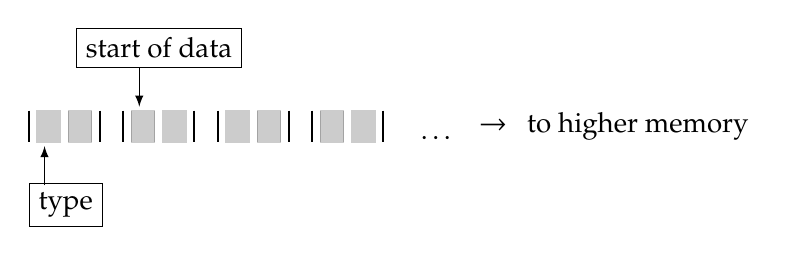
\begin{tikzpicture}
        \foreach \n in {0,...,3}
        {
            \draw [xshift=1.2*\n cm,thick] (0,.4cm)--(0,-.0cm);
            \draw [xshift=1.2*\n cm,fill, opacity=0.2] (+.1,0.4) rectangle (+.4,-.0) {};
            \draw [xshift=1.2*\n cm,fill, opacity=0.2] (+.5,0.4) rectangle (+.8,-.0) {};
            \draw [xshift=1.2*\n cm,thick] (.9,.4cm)--(0.9,-.0cm);
            \coordinate (C\n) at (1.2*\n cm, .2);
        }
        \node[right=1.6cm of C3, anchor=north] (N0) {$\dots$};
        \node[right=2cm of C3] (N1) {$\rightarrow$};
        \node[right=0 of N1] (N2) {to higher memory};
        \node[draw, below= of C0.west,anchor=west] (N3) {type};
        \node[draw, above=1.2cm of C1.west,anchor=west] at (0.6,0) (N4) {start of data};
        \draw[-latex] ($(N4)+(-0.25,-0.25)$) -- ++(0,-.5);
        \draw[-latex] ($(N3.west)+(0.2,0.25)$)  -- ++(0,.5) ;
    \end{tikzpicture}  
    \caption{\textit{Memory structure of a typed scalar}}
    \label{fig:05_01}
\end{figure}
 

We implement a scalar through the defining word

\begin{lstlisting}
    : SCALAR ( type--)
       CREATE DUP , #BYTES ALLOT
       DOES> DUP@ SWAP 2+ SWAP ; ( -- adr t )
\end{lstlisting}

The word \bc{SCALAR} is used as
\begin{lstlisting}
REAL*4   SCALAR X
REAL*8   SCALAR XX
COMPLEX  SCALAR Z
DCOMPLEX SCALAR ZZ
  etc.
\end{lstlisting}

\subsection{Defining several scalars at once}
\TallC{One} aspect of the FORTH method of handling variables, that seems strange to programmers familiar with Pascal, BASIC, or FORTRAN, is that \bc{VARIABLE}, \bc{CONSTANT} or a new defining word like \bc{SCALAR} need to be repeated for each one defined, as above. That is, such defining words generally do not accept name-lists.

This idiosyncracy can be traced to FORTH's abhorrence of variables:
\begin{itemize}
    \item Easily read (and maintained) FORTH code consists of short definitions with few (generally $\leq$ 4) numbers on the stack. Such programs have small use for variables, especially since the top of the return stack can serve as a local variable.
    \item In FORTH as in BASIC, variables tend to be global and hence corruptible. The variables in a large program can have unmnemonic names or names that do not express their meaning simply because we run out of names.
    \item Experienced FORTH programmers tend to reserve named variables for such special purposes as vectoring execution.
    \item The standard FORTH kernel therefore discourages named variables by making them as tedious as possible.
\end{itemize}

Most objections to variables can be resolved by making them local. Local variables are relatively easy to define in FORTH: a straightforward but cumbersome method for making "headerless" words is given in Kelly's and Spies's book\footnote{M.G. Kelly and N. Spies, \textit{Forth, a Text and Reference} (Prentice-Hall, New Jersey, 1986), p. 324 ff.}.

HS/FORTH\footnote{Harvard Softworkts, PO. Box 69, Springboro, Ohio 45066 Tel: (513) 748-0390.} provides beheading in a particularly simple form: \bc{BEHEAD' NAME}, or \bc{BEHEAD" NAME1 NAME2}.

Used after \bc{NAME} has been invoked in the words that need to reference it, \bc{BEHEAD'} removes \bc{NAME}'s dictionary entry leaving pointers and code fields intact and recovering the unused dictionary space. The more powerful word \bc{BEHEAD"} does the same for the range of dictionary entries \bc{NAME1 ... NAME2}, inclusive.

Beheading variable or constant names makes them local to the definitions that use them; they cannot be further accessed -or corrupted- by later definitions. (Pountain\footnote{Dick Fountain, "Object-oriented FORTH", Byte Magazine, 8/86; \textit{Object-oriented FORTH} (Academic Press, Inc., Orlando, 1987).} has given yet another method for making variables local, using a syntax derived from "object-oriented" languages such as SMALLTALK.)

Variables are essential for scientific programming. Since we must often have more than two variables, it is silly to repeat \bc{SCALAR}. A simple way to allow SCALAR to use a list is

\begin{lstlisting}
    :SCALARS ( n -- )
      SWAP 0 DO DUP SCALAR LOOP DROP ;
    \ Examples:
    \ 2 REAL*4  SCALARS  A  B
    \ 5 COMPLEX SCALARS XA XB XC XD XE
\end{lstlisting}

I find the use of \bc{SCALARS} with modifiers and lists more convenient and readable than many repetitions of \bc{SCALAR}. Its resemblance to FORTRAN (thereby helping me live with my FORTRAN-inspired habits) is pure coincidence. Although possible to use a terminator (",\eg) rather than a count (to define the variable list) I feel it is desirable for the programmer to know how many variable names he has supplied, hence the counted version.

\subsection{Generic access}
\TallC{A} major theme of FORTH is to replace decisions by calculation henever possible\footnote{Leo Brodie, \textit{Thinkning FORTH} (Prentice-Hall, Inc., Englewood Cliff, NJ, 1984), p. 118ff. See also J.V. Noble, "Avoid Decisions", \textit{Computers in Physics} 5,4 (1991) 386.}. This philosophy usually pays dividends in execution speed and brevity of code.

But there is an even more important reason to avoid \bc{IF ... THEN} decisions, especially when working with modern microprocessors. CPUs like 80x86 and MC680x0 achieve their speed in part by pre-fetching instructions and storing them in a queue in high speed on-chip cache memory. A conditional-branch machine instruction (the crux of \bc{IF ... THEN}) empties the queue whenever the branch is taken. Branches should be avoided because they slow execution far more than one might expect based on their clock-counts alone.

To replace decisions, we use the standard FORTH technique of the execution array (analogous to the familiar assembly language jump table). This lets us compute from the type descriptor which fetch or store to use.

\TallC{We} now define \bc{G@} and \bc{G!} as execution arrays using\footnote{HS/PORTH uses a word pair \bc{CASE: ... ;CASE} that performs the same task as \bc{G: .. ;} below. \bc{G:} was inspired by Michael Ham (\textit{Dr. Dobb's Journal}, October 1986).} anexecution-array-defining word \bc{G:}

\begin{lstlisting}
    : G: CREATE ]
       DOES> OVER + + @ EXECUTE ; ( t -- )
    G: G@ R32@ R64@ X@ DX@ ;
    G: G! R32! R64! X! DX! ;
\end{lstlisting}

assembled from components of the FORTH compiler. That is, the ordinary colon \bc{:} might have the high-level definition (shorn of error detection)

\begin{lstlisting}
    : : CREATE ] DOES> @ EXECUTE ;
\end{lstlisting}

\bc{CREATE} makes the new dictionary entry, and \bc{]} switches to
compile mode. \bc{DOES>} specifies the run-time action (recall any word created by \bc{CREATE} leaves its parameter field address
\textbf{-pfa-} on the stack at run-time, \textit{prior} to the actions following \bc{DOES>}). In the case of \bc{:} the run-time action is to fetch the pfa of the new word and execute it. At run-time, words defined using \bc{G:} add twice the type descriptor to the pfa (to get the offset into the array) then fetch the desired address and \bc{EXECUTE} it.

Microprocessors like the MC680x0 and 80386 that can address large, level memories require no further elaboration for \bc{G@} and \bc{G!}. However, if large arrays are to be addressed within the segmented memory addressing protocol of the 8086/80286 chips, we would have to define \bc{G@} and \bc{G!} to use the "far" forms of addressing words\footnote{Consult, \eg, LJ. Scanlon, \textit{op. cit.}; or R. Lafore, \textit{op. cit.} HS/FORTH defines "far" access operators, \bc{@L} and \bc{IL} of all types, that expect a "long" address on the stack. For example, \bc{CODE R32®L DS POP. FWAIT. DS:[BX] DWORD-PTR. FLD. END-CODE}}. For example, in HS/FORTH such words as \bc{R32@L} expect a segment paragraph number and offset (32 bits total) as the complete address of the variable being fetched to the 87stack. In that case we modify the definition of \bc{SCALAR} to include the segment paragraph number (seg) in the definition (\bc{LISTS} is nonstande - it is HS/FORTH's name for the portion of the dictionary containing the word headers)

\begin{lstlisting}
    : SCALAR (type - -)
    CREATE DUP , \make header ,type
    #BYTES ALLOT \reserve space
    DOES > > R
    [ LISTS @] LITERAL (- - sag)
    R@ 2 + (- - seg off)
    R> @ - (--segofltype)
    \ Ex: BEAU-4' SCALAR x
\end{lstlisting}

\subsection{The intelligent floating point stack (ifstack)}
\TallC{The} \textbf{ifstach} is a more complex data structure than either a simple fstack or the parameter/retum stacks. When a typed datum is placed on the ifstack its type must be placed there also.

But the typed data have varying lengths, from 4 to 16 bytes. We can deal with this two different ways: either \bc{ALLOT} enough memory to hold a stack of the longest type, making each position on the ifstack 18 bytes wide (to hold datum plus type); or manage the ifstack as a modified heap, with the address of a given datum being computable from the ifstack-pointer and the data type.

The 18-byte wide ifstack wastes memory, but is easy to program. (In retrospect, this is exactly the method I used to program adaptive numerical quadrature\footnote{J.V. Noble, "Scientific Computation in FORTH". \textit{Computers in Physics} 3 (1989) 31; and Ch 8.1.5 of this book.}.) After several false attempts I settled on the fixed-width ifstack. High level FORTH code for this variant is given below.

\begin{lstlisting}
    \ TYPED DATA STACK MANAGER
    TASK FSTACKS
    FIND CP@ 0=
    ?( FLOAD COMPLEX.FTH )

    \ define data-type tokens
    0 CONSTANT REAL*4
    1 CONSTANT REAL*8
    2 CONSTANT COMPLEX
    3 CONSTANT DCOMPLEX

    CREATE #bytes 4 C, 8 C, 16 C,
    : #BYTES #bytes + C@ ; 
    ( type -- length in bytes )

    \define scalar and scalars
    : SCALAR        ( type -- ) 
        CREATE DUP , #BYTES ALLOT 
        DOES> DUP@ SWAP 2+ SWAP ;

    ( -- seg off type )
    \ say: REAL*4 SCALAR X
    : SCALARS ( n type -- )
        SWAP 0 DO DUP SCALAR LOOP
        DROP ;
    \ say: 4 DCOMPLEX SCALARS XA XB XC XD

    \ definitions for the parallel stack of types and data 
    \ Brodle, TF (Brady, NY, 1984) p. 207.

    CREATE FSTACK 2018' 2+ ALLOT
    \ 2 tos-pointer, 20 18-byte cells
    : FS.INT FSTACK 0! ;
    : EMPTY         ( -- seg off )
        [ LISTS @ ] LITERAL
        FSTACK DUP@ 18 * 2+ + ;
    : >FS ( seg off type -- ) \ say: X >FS
        >R >EMPTY ( -- seg off seg' off )
        R@ OVER ! \ store type on ifstack

FS> ( seg off type -- ) \ say: X FS>
FSTACK 1-I              \ dec ifstack ptr
>R >EMPTY               ( -- seg off seg' off' )
DUP@ R@ =               \ srce.type = dest.type ? 
IF 2+ DSWAP             ( -- seg' off' sef off )
R> #BYTES               ( -- seg' off' sef off n )
CMOVEL                  \ move data from ifstack
ELSE RDROP CR 
    ." ATTEMPT TO STORE TO
    WRONG DATA TYPE" ABORT
THEN ;

\ execution-array defining word
\ HS/FORTH has the faster
\ CASE:...;CASE pair for the same job

: G: CREATE ] DOES> OVER + +
    @EXECUTE ; ( t -- )

G: G@ R32@L R64@L X@L DX@L ;
G: G! R32!L R64!L X!L DX!L ;
\ move data from ifstack to/from FPU
: FS>F ( -- t 87: -- x )
    FSTACK 1- !  \ dec ifstack ptr
    >EMPTY      ( -- seg off )
    DUP@ >R 2+
    R@ ( sef off' type )
    G@ R> ;
\ move data from ifstack to 87stack, leave type

:F>FS (t-- 87:x--)
    >R >EMPTY   ( -- sef off )
    R@ OVER!
    2+ R> ;     ( -- sef off' type)
\end{lstlisting}
 

The stack comments and comments should make the preceding code self-explanatory.

\subsection{Unary and binary generic operators}

\TallC{We} want to define generic unary and binary operators whose run-time action selects the desired operation using information contained in the ifstack. A unary operator such as \bc{FNEGATE} or \bc{FEXP} expects one argument and leaves one result. With a floating-point coprocessor (FPU) the only distinction is between real or complex. This distinction is contained in the second bit of the type descriptor, which we exhibit in Table 5-1 on page 101, in binary notation.

Real and complex can then be distinguished via the code fragment

2 AND ( type -- 0 = real| 2 = complex )

% Table 5-1
\begin{table}
    \centering
    \caption{\textit{Bit-patterns of data type descriptors}}
        \bigskip
    \label{tbl:09_01} 
    \setlength{\tabcolsep}{30pt}
        \begin{tabular}{|lll|}
            \hline
            & &\\
            \textbf{Type} & \textbf{BINARY} & \textbf{representation} \\
            & &\\
            REAL*4     &  00000000 & 00000000 \\
            & &\\
            REAL*8     &  00000000 & 00000001 \\
            & &\\
            COMPLEX    &  00000000 & 00000010 \\
            & &\\
            DCOMPLEX   &  00000000 & 00000011 \\
            &&\\
            \hline 
        \end{tabular}
\end{table}


Since most unary operators produce results of the same type as their argument, we write a defining word for generic unary operators:

\begin{lstlisting}
: GU: CREATE ] DOES>    ( -- pfa )
    FS>F ( -- pfa t )   \ get data
    UNDER 2 AND +       ( -- t adr )
    @ EXECUTE           \ do it
    F>FS ;              \ return ans.
\end{lstlisting}

When we use \bc{GU:} in the form
\begin{lstlisting}
GU: GNEGATE FNEGATE XNEGATE ;
\end{lstlisting}

\bc{CREATE} produces a dictionary entry for \bc{GNEGATE; ]} turns on the compiler so the previously defined words \bc{FNEGATE} and \bc{XNEGATE} have their addresses compiled into \bc{GNEGATE}'s parameter field; and \bc{DOES>} attaches the run-time code. The run-time code converts the real/complex bit into an offset, 0 or 2 which is added to the address of the daughter word to get the address where the pointer to the actual code is stored. This pointer is fetched and \bc{EXECUTE}d.

A few unary operators like \bc{XABS} (complex absolute value) return real values from complex arguments. If we want to use \bc{GU:} to define, say, \bc{GABS}, we must remember to redefine \bc{XABS} so it zeros the second bit of the type descriptor left on the stack, before returning its result to the ifstack. This is just a \bc{1 AND} so is fast.

A binary operator (one that takes two arguments) expects its arguments \textit{and} their types on the ifstack. There is no distinction between single- and double-precision arithmetic on most numeric coprocessors. However, the result must leave the proper type-label on the stack. Here is what we want to happen, illustrated in fig. 5-2 as a matrix \regc{TYPE(arga, argb))}
% fig. 5-2 
\begin{figure}
    \center
    \label{fig:05_02}
    \newcolumntype{x}[1]{>{\let\newline\\\arraybackslash\hspace{0pt}}p{#1}}
    \setlength{\extrarowheight}{0.1cm}
    \begin{tabular}{|llm{7cm}|}
        \hline
        &&\\
        TYPE\textsubscript{ab} && \\
        &&
        \begin{tabular}{ x{0.8cm}x{0.8cm} x{0.8cm} x{0.8cm} x{0.8cm} }
            \textsubscript{\space \space b}&&&&\\
            %\textsuperscript{b}&&&&\\
             
            \diaghead(-3,2){\hskip \hsize} a & R & D & X & DX \\
            \cline{2-5}
            \multicolumn{1}{ x{0.8cm}|}{R  }&  R & R & X & X \\
            \multicolumn{1}{ x{0.8cm}|}{D  }&  R & D & X & DX \\
            \multicolumn{1}{ x{0.8cm}|}{X  }&  X & X & X & X \\
            \multicolumn{1}{ x{0.8cm}|}{DX }&  X & DX & X & DX 
        \end{tabular}
        \\
        &&\\
        \hline
    \end{tabular}
    \caption{\textit{Types resulting from 2-argument operators}}
\end{figure}

\leftbar[1\linewidth]
Note: this protocol avoids misleading precision for the results of computations. It seems more scientific than FORTRAN's "convert intermediate results to the precision of the highest-precision operand" protocol.
\endleftbar

If we think of the indices and entries in Fig. 5-2 as numbers 0, 1, 2, 3 (so we can use them as indices into a table) rather than as letters, a simple algorithm emerges: the first bit of the result is the logical-AND of the first bits of the two operands, and the second bit of the result is the logical-OR of their second bits. Although we would program this in assembler for speed, the high-level definition is

\begin{lstlisting}
: NEW.TYPE  ( a b -- a2 + b2 + a1b1 )
    DDUP        ( -- a b a b        )
    AND         ( -- a b ab         )
    1 AND       ( -- a b [ab]1      )
    -ROT OR     ( -- [ab]1 a+b      )
    2AND        ( -- [ab]1 [a+b]2   )
    + ;         ( -- a2 + b2 + a1b1 )
\end{lstlisting}

Since only logical operations are used. \bc{NEW.TYPE} is faster than table lookup or branching. Note that in programming this key word we have obeyed the central FORTH precept: "Keep it simple!" by choosing a data structure (the numeric type tokens 0-3) that is easily manipulated.

We will also need a way to select the appropriate operator from a jump table of addresses. Given that the precision (internal) is irrelevant, again all that matters is whether the number is real or complex, \ie the second bits of the numbers. The first operation must then be to divide by 2 (right-shift by one bit). We then have the matrix of FYig. 5-3 below
% Fig. 5-3 
\begin{figure}
    \center
    \label{fig:05_03}
    \begin{tabular}{|lll|}
        \hline
        && \\
        && \\
        \begin{tabular}{ccc}
            & 0 & 1 \\
            \cline{2-3}
            \multicolumn{1}{c|}{0  }&  RR & RX \\
            \multicolumn{1}{c|}{1  }&  XR & XX \\
        \end{tabular}
        %& $\rightarrow $ &
        & $ \xrightarrow{\hspace*{1cm}} $ &
        \begin{tabular}{ccc}
            & 0 & 1 \\
            \cline{2-3}
            \multicolumn{1}{c|}{0  }&  0 & 1 \\
            \multicolumn{1}{c|}{1  }&  2 & 3 \\
        \end{tabular}
        \\
        &&\\
        &&\\
        \hline
    \end{tabular}
    \caption{\textit{Operator selection matrix}}
\end{figure}
where RR stands for real-real, \textit{etc.} The numerical elements are generated as \regc{2*J+I}. This leads to the word

\begin{lstlisting}
    : WHICH.0P ( a b -- c )
        2/ SWAP 2 AND + ;
\end{lstlisting}

Thus we come to the binary generic-operator defining word
\begin{lstlisting}
    : GB: CREATE ] DOES>        ( -- pfa )
        FS>F FS>F               ( -- pdf t0 t1 )
        NEW.TYPE UNDER          ( -- t' pfa t' )
        WHICH.OP 2* +           \ make result-type
            @ EXECUTE           \ select binop
        F>FS ;                  \ save result
    \say: GB: G*   F*  F*X  X*F  X* ;
\end{lstlisting}

The generic multiply \bc{G*}, \eg, picks out, at run-time, which of four routines to use. By using only logical or shift operations we have made even the high-level definitions fairly quick in comparison with the times of floating point operations.

The only instance where one might forego the overhead penalty paid for the convenience of generic coding would be in nested inner loops, such as occur in matrix operations. Here it might pay to code four inner loops, one for each type, and then access them generically, \eg

\begin{lstlisting}
    : RLOOP      ... real     words ... ;
    : DRLOOP     ... dreal    words ... ;
    : XLOOP      ... complex  words ... ;
    : DXLOOP     ... dcomplex words ... ;
    G: GLOOP  RLOOP DRLOOP XLOOP DXLOOP ;
\end{lstlisting}

\section{Arrays of typed data}

\TallC{Numerical} arrays represent a frequently encountered characteristic feature of scientific programming. Arrays \textit{per se} are hardly foreign to FORTH. Arrays of typed data are novel, however, and therefore worth elaborating. Following Brodie's advice(\TF, p. 48ff) we first specify the "user interface" (matrix notation) and then proceed to implementation.

\section{Improved (FORTRAN-like) array notation}
\TallC{Something} like V(15) --the 15'th element of V-- is the commonest notation for array elements in high-level languages because lineprinters and terminals do not easily recognize subscripts. In FORTH, the most natural notation would be postfix (RPN), \bc{15 V} --but this is both hard to read and unintuitive\footnote{Other authors have noted this and proposed more readable matrix notations. See, \eg, Joe Bentham, "FORTH and the Fast Fourier Transform" \textit{Dr. Dobb‘s Journal}, September, 1984, p. 34. Also Dick Pountains's book \textit{Object-oriented FORTH (op cit.)} uses an array naming convention with brackets.}. That is, \bc{15 V} does not say, immediately and unambiguously, "I am the 15th element of the array V !"

FORTH's idiosyncrasies forbid saying V(15) because the parser recognizes V(15) as a single word\footnote{Recall that the standard FORTH delimiter is the ASCII blank (20h = 32d).}. Since we want the 15 to be parsed, we would have to modify the FORTRAN-ish notation to Vdot(dot15) or V(dot15dot), where dot stands for a blank space (ASCII 32). Unfortunately, "(" is a reserved word. While we might place the matrix definitions in a separate vocabulary --which would let us redefine anything we want-- "(" is too useful as a comment delineator to dispense with.

This leaves the second possibility, where "(" becomes part of the array name, \regc{V(}. To make \regc{V(dot15dot)} work,")" must become an operator --unless we want to leave postfix notation entirely, with all the complication that would entail\footnote{See, \eg,L. Brodie, \textit{Thinking FORTH (op. cit.)} p. 113ff.}. Since ")" is not a reserved word, nothing in principle prevents defining it as an operator. However, such usage would conflict with comments.

The square braces, [ ], are commonly used in matrix notation; however both are reserved FORTH words, \ie forbidden. This leaves the curly braces { }, which are unused by FORTH.

Of the two possible forms, Vdot{dot15} or V{dot15dot}, the latter has the
advantage that the opening brace, \regc{\{}, is only part of the name, but
reminds us that the name \regc{V\{} is an array, exactly as names ending with
\bc{\$} are strings, \textit{etc}. The notation suggests a further mnemonic
refinement, namely to place \bc{\{\{} and \bc{\}\}} at the ends of
2-dimensional arrays, as in $\mathbf{M\{\{\bullet \;3 \bullet 5 \;\bullet \}\}}$.

How will this notation operate? Clearly, to place the (generalized) address of the n'th element (of a 1-dimensional array) on the stack we would say

\begin{align*}
    V\{\bullet \;n \;\bullet\}
\end{align*}

whereas

\begin{align*}
    M\{\{ \bullet \;m \bullet n \;\bullet\}\}
\end{align*}

should analogously place the address of the m,n'th element of a 2-dimensional array on the stack.

\subsection{Large matrices}
\TallC{The} defining word \bc{SCALAR} given in \S2 above allots space in the dictionary --for most FORTHs, code + data must fit here-- or in the LISTS segment of HS/FORTH (part of the dictionary). This is OK for variables, but not for arrays, since even a modest matrix would exhaust the ( $\leq$64 Kbyte) LISTS segment.

A \bc{REAL*4} matrix uses 4 bytes per ellement. The largest such array that can be stored in a 65,536 (\ie, $2^{16}$) -byte segment is 128x128. This is the largest array that can be addressed with unsigned 16-bit numbers. On the other hand, a filled IBM PC/XT clone has 64 Kbytes of memory under MS-DOS. Even a generous F0RTH kernel (plus DOS) takes up less than 150 K; hence 450 K is available to hold large arrays. Up to 8 Mbytes can be added as EMS storage, assuming a suitable memory management scheme\footnote{See, \eg, Ray Duncan, "FORTH support for Intel/Lotus expanded memory", \textit{Dr. Dobb's Journal}, August 1986; also, John A. Lefor and Karen Lund, "Reaching into expanded memory", \textit{PC Tech Journal}, May 1987.}. That is, in principle one could tackle matrix problem of order 350x350. What about speed? The dominant term is solving linear equations by --say-- Gaussian elimination with partial pivoting is
\[
T = \frac{1}{3} mn^{3}
\]
where m is the time for 1 multiply and 1 add, and n is the order of the matrix. We should also include the fetch + store time, since the bus bandwidth is as much a limiting factor as the FPU arithmetic speed. For the 8086/8087 the time $m$ is of order 400 clock cycles. Thus the asymptotic execution time on a 10 MHz machine should be of order 10 minutes for n = 350.

On the 80386/80387 combination running at 25 MHz, the execution time for the same problem should be only 2.3 minutes or so. Thus it would be practical (\ie, execution time $\approx$ 1 hour) on such machines, even without special equipment such as the IIT 80c387, or an array co-processor, or a faster procedure such as Strassen's algorithm (see Ch. 4 \S8), to tackle $10^{3} x 10^{3}$ dense matrix problems.

The crucial question therefore, is memory. The Intel machines were designed around a segmented memory architecture. That is, to avoid having to use (expensive) 32-bit address registers, the 8086/80286 chips were designed to use 16-bit registers. However, these chips have more than 16 external address lines - 20 for the 8086, 24 for the 80286. Thus the absolute address is compounded of two numbers: a \textbf{segment descriptor} and an \textbf{offset}, which must be present in appropriate registers. The segment descriptor is the \textbf{absolute address} of a l6-byte \textbf{paragraph}, divided by 16. The offset is any (unsigned) integer from 0 to $2^{16}-1 = 65,535$ that can fit in a 16-bit register.

The chips contain 4 segment registers: SS (stack segment), CS (code segment), DS (data segment) and ES (extra segment). Five registers, BP, SP, SI, DI, and BX, can be used for offsets, although they are not entirely interchangeable (some have specific functions in some of the more complex machine instructions, such as string operations). Manifestly, since the 8086 can address

$2^{20} = 1,048,576 \textrm{ bytes ("1 megabyte")}$,

the largest segment number is $2^{14}-1 = 16,383$.

A typical (segmented) address is expressed in Intel assembly code
as

\begin{lstlisting}
    CS: [BX + SI + 0008]
\end{lstlisting}

which translates in words to "add the offset in BX to that in SI and then add 8 to get the total offset; take the segment descriptor in CS, multiply by 16 and add to produce the absolute address.

\subsection{Using high memory}
\TallC{HS/FORTH} permits accessing all the memory in a PC/AT (up
to 1 megabyte) in the following manner:
\begin{itemize}
    \item Define a named segment of length 1 byte: this marks the beginning of available memory.
    \item Then tell both FORTH and DOS how much memory you want.
\end{itemize} 

As might be expected, HS/FORTH defines non-standard words (coded as DOS function calls) to use the various DOS service routines that allocate memory, \textit{etc}.\footnote{See, \eg, D.N. Jump, \textit{Programmer's guide to MS-DOS}, rev. ed. (Brady Books, New York, 1987).}

\begin{lstlisting}
    MEMORY 4+ @ S->D
    DCONSTANT MEM.START \ beg. of free memory
    40.960 DCONSTANT MAX.PARS
        \ 40960 = 655360 /16
    : TOTAL.PARS MAX.PARS MEM.START D- ;
        \ # pars of memory available
    1 SEGMENT SUPERSEG
        \ define named segment 1 byte long
    TOTAL.PARS DROP FREE-SIZE
        \ tell DOS and HS/FORTH about it
\end{lstlisting}

Having allocated the memory, how can we address it efficiently? We would like the simplicity of double-length integer arithmetic for computing an (absolute) array address, as in

\begin{lstlisting}
    abs.adr(Aij) = abs.adr(Ainf) + (row.length*I+J) *#BYTES
\end{lstlisting}

However, although the absolute address referenced by a segment and offset is unique, \ie the absolute address in bytes is

\begin{lstlisting}
    abaadr -18'segment + offset,
\end{lstlisting}

the reverse translation, of an absolute address (in bytes) to the segment + offset notation expected by 80x86 processors is \textit{not} unique. This naturally poses a problem when the processor tries to prevent segments from overlapping (protected mode). In such cases, the only answer is a memory management scheme that computes segments and offsets (by brute force) in a non-overlapping fashion. For example, we might define large arrays such that each row has its own segment paragraph.

The 80386 CPU has a third mode that permits direct 32-bit addressing of 4 gigabytes (albeit few computer users have quite this much fast memory available). A scheme for addressing large amounts of RAM in 80386 machines (without leaving MS-DOS) has been discussed in \textit{Dr Dobb's Journal}\footnote{See, \eg, Al Williams, "DOS + 386 = 4 Gigabytes", Dr. Dobb's Journal, July 1990, p. 62.}.

For 8086 PC's and/or real-mode programming on 80286 + machines, we can merely ignore whether segments overlap. Oddly, standard assembly programming books\footnote{C. Morph and M. Waite, \textit{8086/8088 16-bit microprocessor primer} (Byte/McGraw-Hill, Peterborough, 1982); L. Scanlon, \textit{IBM PC \& XT assembly language: a guide for programmers} (Brady/Prentice-Hall, Bowie, Md., 1983); R. Lafore, \textit{Assembly language primer for the IBM PC \& XT} (Plume/Waite, New York, 1984).} omit this way of addressing segmented memory.

The 8086 permits 32-bit addressing as long as we translate 32-bit addresses to the segment + offset notation expected by the 80x86 processors in real mode. A word that performs this conversion is \bc{SEG.OFF}, defined as

\begin{lstlisting}
    : >SEG.OFF          ( d -- seg off )
        OVER 15 AND     (   --   d off )
        -ROT D16/ DROP  (   -- off seg )
        SWAP ;
\end{lstlisting}

The 32-bit address is placed on the stack as a double-length integer, with the low-order (\ie offset part) above the segment part. The phrase \bc{OVER 15 AND} saves bits 0-3 (of the 32-bit address); \bc{-ROT D/16 DROP} then shifts the (32-bit) address right 4 bits and drops the least-significant part, to produce the offset. This conversion method produces offsets in the range 00-0F (hex), that clearly have nothing to do with the original offsets (that led to the 32-bit absolute address \textit{via} 16*seg + off ).

\subsection{A general typed-array definition}
\TallC{For} the new syntax to work the word \bc{\}} must compute the addresses of the n'th element of \bc{V\{} from the information on the stack, and \bc{\}\}} must do the same for \bc{M\{\{}. In order to encompass matrices of typed data we specify that the results of the phrases \bc{V\{ n \}}and \bc{M\{\{ m n \}\}} be to leave the generalized address on the parameter stack, \ie to leave the stack picture ( -- seg off type), exactly as with \bc{SCALARS}.

Before we can define \bc{\}}, however, we must specify the data: structure it operates on, \ie the array header.

Once again we begin with the user interface. We can opt for maximum generality or maximum simplicity. My first attempt fell into the first category, permitting the user to define a named segment of given length and to define an array in that segment. Lately I realized this generality accomplishes little, so have abandoned it. All arrays will be defined in the heap, named SUPERSEG as above. To define a length-50 \bc{1ARRAY} of 4-byte number we will say

\begin{lstlisting}
    50 LONG REAL*4 1ARRAY V{
\end{lstlisting}

Now, before we work out the mechanics of \bc{1ARRAY}, we imagine that an array will be stored as in Fig. 5-4 below:

The proposed data structure consists of an 8-byte header (the array descriptor) in the dictionary (\regc{LISTS} in HS/FORTH), with the body of the array stored elsewhere. The array descriptor points to the absolute address of the array data (body).
% Fig. 5-4 
\begin{figure}
    \center
    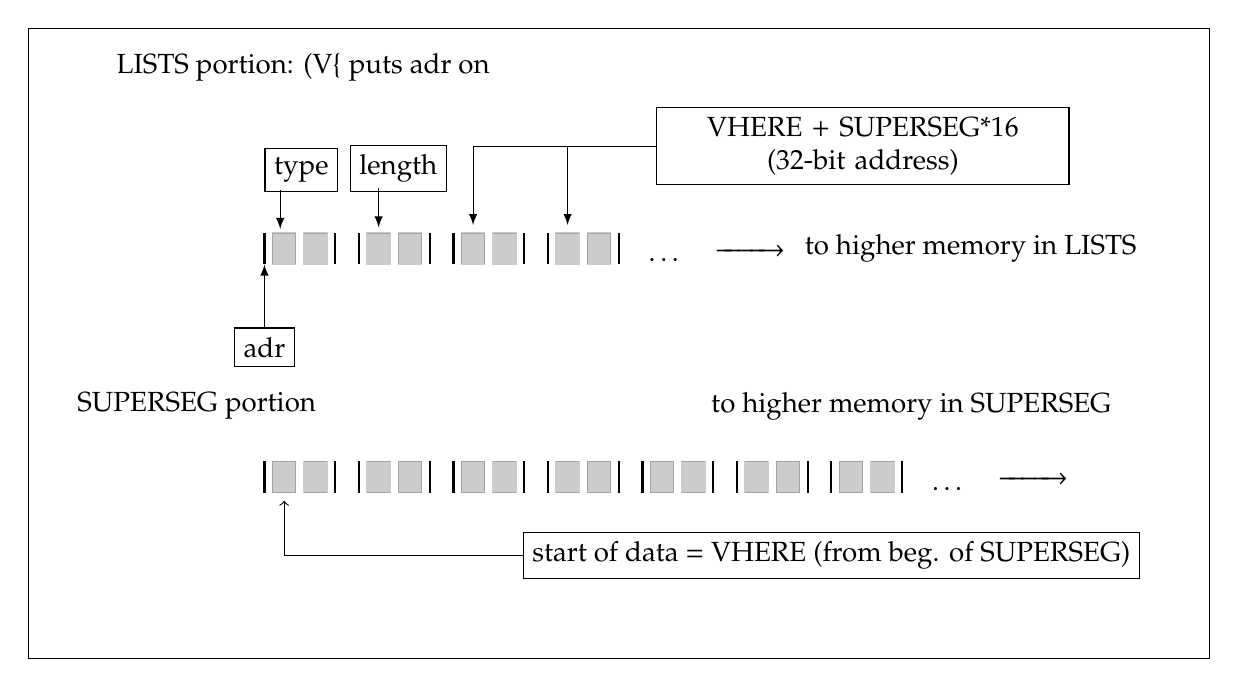
\begin{tikzpicture}
        \draw (-3,-5) rectangle (12,3.0);
        \node[align=left, anchor=west] at (-2,2.5) {LISTS portion: (V\{ puts adr on};
        \node[align=left, anchor=west] at (-2.5,-1.8) {SUPERSEG portion};
        \foreach \n in {0,...,3}
        {
            \draw [xshift=1.2*\n cm,thick] (0,.4cm)--(0,-.0cm);
            \draw [xshift=1.2*\n cm,fill, opacity=0.2] (+.1,0.4) rectangle (+.4,-.0) {};
            \draw [xshift=1.2*\n cm,fill, opacity=0.2] (+.5,0.4) rectangle (+.8,-.0) {};
            \draw [xshift=1.2*\n cm,thick] (.9,.4cm)--(0.9,-.0cm);
            \coordinate (C\n) at (1.2*\n cm, .2);
            \coordinate (CB\n) at (1.2*\n cm, 0);
            \coordinate (CT\n) at (1.2*\n cm, 0.4);
            \coordinate (FT\n) at (1.2*\n +0.25, 0.5);
            \coordinate (ST\n) at (1.2*\n +0.5, 0.5);
        }
        \node[right=1.5cm of C3, anchor=north] (N0) {$\dots$};
        \node[right=2cm of C3] (N1) {$\xrightarrow{\hspace*{0.7cm}}$};
        \node[right=0 of N1] (N2) {to higher memory in LISTS};
        \node[draw, above= of C0.west,anchor=west] (N3) {type};
        \node[draw, above= of ST2] at (1.7,-0.08) (N4) {length};
        \node[draw, below= of C0.west] (N5) {adr};
        \node[align=center, draw, text width=5cm] at (7.6,1.5) (N6) {VHERE + SUPERSEG*16\\(32-bit address)};
        \draw[-latex] ($(N4)+(-0.25,-0.25)$) -- ++(0,-.5);
        \draw[-latex] ($(N3.west)+(0.2,-0.25)$)  -- ++(0,-.5) ;
        \draw[-latex] (N5.north)  -| (CB0) ;
        \draw[-latex] (N6.west)  -| (FT3) ;
        \draw[-latex] (N6.west)  -| (FT2) ;

        \foreach \n in {0,...,6}
        {
            \draw [yshift=-2.9cm, xshift=1.2*\n cm,thick] (0,.4cm)--(0,-.0cm);
            \draw [yshift=-2.9cm, xshift=1.2*\n cm,fill, opacity=0.2] (+.1,0.4) rectangle (+.4,-.0) {};
            \draw [yshift=-2.9cm, xshift=1.2*\n cm,fill, opacity=0.2] (+.5,0.4) rectangle (+.8,-.0) {};
            \draw [yshift=-2.9cm, xshift=1.2*\n cm,thick] (.9,.4cm)--(0.9,-.0cm);
            \coordinate (C\n) at (1.2*\n, -2.9+0.2);
            \coordinate (FB\n) at (1.2*\n +0.25, -2.9 -0.1);
            \coordinate (st\n) at (1.2*\n +0.75, -2.9 +0.5);
        }
        \node[right=1.5cm of C6, anchor=north] (n0) {$\dots$};
        \node[right=2cm of C6] (n1) {$\xrightarrow{\hspace*{0.7cm}}$};
        \node[draw, below=0.7cm of C6] (n3) {start of data = VHERE (from beg. of SUPERSEG)};
        \draw[->] (n3.west) -| (FB0);
        \node[above=0.6cm of st4, anchor=west] (n2) {to higher memory in SUPERSEG};
    \end{tikzpicture} 
    \label{fig:05_04}
    \caption{\textit{Structure of a 1-dimenslonal array in \regc{SUPERSEG}}}
\end{figure}

The array-defining word 1ARRAY must perform the following
tasks:

\begin{itemize}
    \item place the length and type of the data in the first two cells 4 bytes) of the array descriptor.
    \item place the 32-bit address (start of data) in the next two cells 4 bytes) of the array descriptor.
    \item allot the necessary storage in \bc{SUPERSEG}.
    \item at run-time, place the generalized address, length and type on the parameter stack.
\end{itemize}

The start of data is handled by \bc{VHERE}, a word that puts the next vacant (32-bit) address in \bc{SUPERSEG} on TOS.

We define \bc{VALLOT} to keep track of the storage used by arrays. \bc{VALLOT} increments the pointer in \bc{VHERE} (and aborts with a warning if the segment length is exceeded).

We first define some auxiliary words:
\begin{lstlisting}
    MEMORY 4 + @
    S-> D DCONSTANT MEM.START
        \ beg. of free memory
    40.960 DCONSTANT MAX.PARS \ 40960 = 655360/16
    : TOTAL.PARS MAX.PARS   MEM.START D- ;
        \ # pars avail. mem.
    1 SEGMENT SUPERSEG        \ named seg. 1 byte long
    TOTAL.PARS DROP
        FREE-SIZE             \ tell DOS and HS/FORTH

    DVARIABLE VHERE>
    : INIT.VHERE> 0.0 VHERE> D! ;
    INIT.VHERE>
    : VHERE ( -- d.offset ) VHERE> D@ ;
    : D4/   D2/ D2/ ;
    : D16/  D4/ D4/ ;

    : TOO-BIG? VHERE >SEG.OFF
        0 AND TOTAL.PARS D>
        ABORT" INSUFFICIENT ROOM IN SUPERSEG" ;
        \ check whether new value of VHERE> passes end
        \ of SUPERSEG

    : VALLOT ( d.#bytes -- )
        VHERE  D+ DDUP TOO.BIG?
        VHERE> D! ;

    \ Array-defining words
    \ Ex: 50 LONG REAL*4 1ARRAY V{
    \ V{            (   -- adr )
    \ V{ 17 } >FS   (:: -- V[17])

    : LONG DUP ;
    FIND D, 0= ?( :D, SWAP , , ; )
        \ conditionally compile D,
    :1ARRAY ( || t -- )
        CREATE UNDER D,  \ t,| into 1st 4 bytes { -- |t )
        SUPERSEG @ 16 M* \ start of SUPERSEG
        VHERE D+ D,      \ abs. address -> next 4 bytes
        #BYTES M*        ( | t -- #bytes to allot)
        VALLOT ;         \ allot space in the segment
    \ run-time action: ( -- adr )
\end{lstlisting}

We also need some words to go with \bc{1ARRAY}:
\begin{lstlisting}
    :}  (adr n -- seg.off[n] t )
        SWAP DUP@ R > \ type -> rstack
        4+  D@
        ROT R@ #BYTES M*
        D+ >SEG.OFF R > ; ( -- seg.off[n] t )
\end{lstlisting}

Finally, here is a useful diagnostic word

\begin{lstlisting}
    :7TYPE ( t-- ) \ it's ok for this to be slow!
        DUP 0 = IF DROP ." REAL*4"   EXIT THEN
        DUP 1 = IF DROP ." REAL*8"   EXIT THEN
        DUP 2 = IF DROP ." COMPLEX"  EXIT THEN
        DUP 3 = IF DROP ." DCOMPLEX" EXIT THEN
        ." NOT A DEfiNED DATA TYPE" ABORT ;
\end{lstlisting}

\subsection{2ARRAY and \}\} }
\TallC{We} now want to define arrays of higher dimensionality. For example, to define a 2-dimensional array we might say

\begin{lstlisting}
    90 LONG BY 90 WIDE COMPLEX 2ARRAY XA{{
\end{lstlisting}

This leads to the definitions
\begin{lstlisting}
    : BY ; \a do-nothing word for style
    : WIDE * ; (I w -- I*w)
    : 2ARRAY   (I*w t -- ) 1ARRAY ;
\end{lstlisting}

Now let us define \}\} to fetch the double-indexed address:

\begin{lstlisting}
    : }} ( adr m n -- a[m*I+n] t)
        >R OVER 2+ @ ( -- adr m I*w)
        * R> + } ;
\end{lstlisting}

By correct factoring (putting some of the work into \bc{WIDE}) we achieved an easy definition of \bc{2ARRAY}. Careful factoring also let
us define \}\} in terms of \}.

\section{Tuning for speed}

Some of the words in our typed-data/matrix lexicons should be optimized or redefined in machine code. Accessing matrix elements imposes a non-trivial overhead on matrix operations. We can reduce the execution time with inline code, either in the traditional FORTH manner via selected assembler definitions, or with a recursive-descent optimizer such as HS/FORTH's\footnote{J.S. Callahan, \textit{Proc. 1988 Rochester FORTH Conference} (Inst. for Applied FORTH Research, Inc., 1988), p. 39.}.

Experience teaches that optimization is most fruitful (most bang for the buck) applied to entire inner loops and other selected areas of code, rather than to access words \textit{per se}. By hand-coding the innermost loop in matrix inversion and FFT routines, one achieves programs that run in (asymptotically) minimum time on the 8086/8087 chip set.

\TallC{Significant} speed increases in data access could perhaps be obtained with multiple code field (MCF) words, as described by Shaw\footnote{G. Shaw, "Forth Shifts Gears, I", \textit{Computer Langmge} (May 1988) p. 67; "Forth Shifts Gears, II", \textit{Computer Language} (June 1988) p. 61; \textit{Proc. 9th Asilomar FORML Conference} (JFAR 5 (1988) 347.)}, and as implemented by HS/FORTH in the words \bc{VAR}, \bc{AT}, \bc{IS}, and variants thereof. The disadvantage of MCF style is that compile-time binding, while faster in execution, loses the flexibility of run-time binding. That is, data types would - as with FORTRAN - be specified at compile-time, and lexicons would be recompiled to run with specific types. Run-time binding as described in this Chapter produces \textit{generic} words that can handle all four standard scientific data types, a major advantage over MCF.

\leftbar[1\linewidth]
FORTH data structures, especially as defined in this Chapter, do little- or no bounds checking, hence do not prevent accidentally overwriting key parts of the operating system.

The new fetch and store words were defined in high-level FORTH for safety. Adding bounds-checking to arrays, at least during the debug cycle, is \underline{strongly recommended} to avoid crashing, or even damaging, the system.
\endleftbar



    % \chapter{Programming Examples}
\startcontents[chapters]
\printcontents[chapters]{}{1}{}

\TallC{This} chapter illustrates how we may apply the floating point extensions of FORTH, developed in preceding chapters, to some standard problems in numerical analysis.

\section{Infinite series}

Frequently we must evaluate a function defined by an infinite sum

\begin{align}
    f(x) = sum_{n=0}^{\infty}c_{n}x^{n}
\end{align}

where $x$ is a real number and $c_n$ is an infinite sequence of coefficients. The extensive mathematical theory\footnote{\textit{The Handbook of Mathematical Functions} ed. Milton Abramowitz and Irene Stegun (Dover Hlications, Inc, New York, 1965) - henceforth abbreviated HMF- is a mine of useful information and references, on this as well as many other aspects of numerical analysis.} of such functions tions can be summarized as follows: the series of terms only have meaning if -for fixed $x$- the sequence of partial sums

\begin{align}
    f_{N}(x) = sum_{n=0}^{N-1}c_{n}x^{x}
\end{align}

has a definite limit.

\subsection{Examples of Infinite series}
\TallC{Perhaps} the formal definitions will seem clearer after some concrete examples. We now examine some divergent an convergent series.

\subsubsection{Divergent examples}
What does it mean to say a series diverges? Consider the serices whose terms are all 1's (that is, $c_n = 1, x = 1$):

\begin{align}
    1 + 1 + 1 + 1 + ...
\end{align}

The partial sum $f_N$ is just $N$, and therefore increases without limit as more terms are added. The series \textit{diverges}.

A harder case is the series whose terms are alternately 1's and -1's:

\begin{align}
    1 - 1 + 1 - 1 + 1 - ...
\end{align}

Depending on how the terms are grouped together, the partial
sums can have any value. Certainly the partial sums do not settle
down to any definite value. The series \textit{diverges}.

Yet a third case is the harmonic series

\begin{align}
    f_{N} = 1 + \frac{1}{2} + \frac{1}{3} + \frac{1}{4} + ... + \frac{1}{N}
\end{align}

It can be shown that for large $N$, $f_{N}$ is approximately $log_{e}(N)$, so the harmonic series \textit{diverges}.

\subsubsection{A convergent example}
Are there ever mes of infinite series that \textit{do} mean something? Obviously, or there could hardly be a theory of them! An example\footnote{This is the examle of Zeno's paradox where you are at one end of a sofa and an attractive person of the opposite gender is at the other end. You move half the distance, then half the remainder. Clearly an an infinite number of moves is necessary to achieve the desired proximity. Thus, according to Zeno, you never get there. According to Eq. 6, however, you \textit{do} get there and in a finite time, to boot!} is $c_{n}=1, x = \frac{1/2}$. Here the partial sums

\begin{align}
f_{0} =& 1                               \\
f_{1} =& 1 + \frac{1}{2}                 \\
f_{2} =& 1 + \frac{1}{2} + \frac{1}{4}   \\
........&........                        \\
\lim_{N\to\infty} f_{N} \equiv \lim_{N\to\infty} \frac{1-(\frac{1}{2})^{N}}{1-\frac{1}{2}} = 2
\end{align}

\textit{do} have a definite limit, so the series converges.

\subsection{Numerical examples of convergent series}
\TallC{How} do we tell whether a series has converged? As a practice matter, we keep adding terms to the partial sum until it no longer changes, within the desired precision. Sometimes this can involve a great many terms, even when the series converges. There exists an extensive mathematical literature on testing for the convergence of an infinite series. Mathematicians have also developed many tricks for accelerating the convergence of slow converging series\footnote{HMF, Ch. 3 6 ff.}. Consulting the literature in difficult cases I strongly recommended - it can save time galore!

As an heuristic exercise, let us write some simple programs to evaluate partial sums and see how convergence works.

first we sum the terms $2^{-n}$ from Eq. 6. The flow diagram is shown in Fig. 6-1 below.

\begin{lstlisting}

SETUP: N=0 SUM=1
BEGIN
?CONTINUE ( 10 more terms?)
WHILE
NO YES
10 0 DO
Exit 2^{-n-1} = 2^{-n} / 2
SUM = SUM + 2^{-n-1}
n = n + 1
LOOP
REPEAT
\end{lstlisting}

Fig. 6-1 \textit{Computing 2 the hard way}

The corresponding program is

\begin{lstlisting}
    15 #PLACES !            \ set F. to 15 digits
    : NEXT.TERM
        ( n -- n+1 :: sum 2^-n -- sum'2^-n-1 )
        F2/ FUNDER F+ FSWAP 1+ ;
    : SET.UP FINIT F=1 F=1 0 ;
    : EXHIBIT CR DUP ." n = " .
        2 SPACES
        FOVER ." sum = " F. ;
    : ?CONTINUE  CR ." Another 10 terms?" ?YN ;
    \ ?YN expects a "y" or "n" from the keyboard and
    \ leaves -1 ( "true" ) if "y" is pressed, 0 if "n"
    : SUM SETUP
        BEGIN EXHIBIT ?CONTINUE
        WHILE 10 0 DO NEXT.TERM LOOP
        REPEAT ;
\end{lstlisting}

This is what a run looks like:

\begin{lstlisting}
FLOAD TEST.SUM Loading TEST.SUM ok
SUM
n = 0  sum = 1.00000000000000
Another 10 terms? Y
n = 10 sum = 1.919902343750000
Another 10 terms? Y
n = 20 sum = 1.99999904632568
Another 10 terms? Y
n = 30 sum = 1.99999999906867
Another 10 terms? Y
n = 40 sum = 1.99999999999909
Another 10 terms? N ok
\end{lstlisting}

The partial sums converge rapidly to 2 (which, as we saw in Ch. 1.1.2 above, is the exact sum).

For a second example, let us sum a standard infinite series representation for $\pi/4$: We note that the function $\tan^{-1}(x)$(that is, arctan(x) ) has the infinite series representation\footnote{HMF, Ch. 4 4.42}

\begin{align}
    \tan{x}^{-1} = x - \frac{x^{3}}{3} + \frac{x^{5}}{5} - \frac{x^{7}}{7} ...
\end{align}

Since a $45^\circ$ right triangle has equal height and base, the tangent of $45^\circ$ is 1 (side opposite over side adjacent). That is\footnote{Since $\pi/4$ radians is 45^{\circ}.},

\begin{align}
    \frac{\pi}{4} \equiv \ta{1}^{-1} = 1 - \frac{1}{3} + \frac{1}{5} - \frac{1}{7} + \frac{1}{9}...
\end{align}

Actually the series Eq. 8 is slowly converging and therefore a poor way to compute $\pi$\footnote{A better method would be to evaluate the series for $x = 1/\sqrt{3}$ which is the tangent of $\pi/6$, or $x = \sqrt{Z-1}, the tangent of $\pi/8$}. But anyway, let us proceed. The flow diagram is now that of Fig. 6-2 below.

\begin{lstlisting}
SETUP: flag=1 n=1 sum=0 (--1n::--O)

BEGIN
    EXHIBIT \ display n, sum
    ?CONTINUE WHILE
    
    DUP S->F 1/F    ( -- fn :: -- sum 1/n )
    SWAP FDUP FSIGN \ transfer sign
    F+              \ sum = sum +
    term
    NEGATE          \ flip sign of f
REPEAT
\end{lstlisting}
Fig. 6-2 \textit{ Computing $\pi/4$ by the infinite series for $\tan{1}^{-1}}

The corresponding program is
\begin{align}
    15 #PIACES ! \ set F. to 15 digits
    : NEXT.TERM ( f 2n+1 -- f1 2n+3 :: sum -- sum1 )
        DUP S->F 1/F SWAP DUP FSIGN F+
        NEGATE SWAP 2+ ;
    : SETUP FINIT F=0 1 1 ;
    : EXHIBIT CR DUP
        ." n = " . Z SPACES
        FDUP F2* F2* ." 4*sum = " F. ;
    : ?CONTINUE ." Another term?' ?YN ;

    : PI/4 SET.UP
        BEGIN EXHIBIT
        ?CONTINUE
        WHILE NEXT.TERM REPEAT ;
\end{lstlisting}

Now we run the program\footnote{Note we have set up to display $x$ rather than $x\4$.}:

\begin{lstlisting}
FLOAD PIBY4 Loading PIBY4 ok
PI/4

n = 1  4*num = Another term? Y
n = 3  4*num = Another term? Y
n = 5  4*num = Another term? Y
n = 7  4*num = Another term? Y
n = 9  4*num = Another term? Y
n = 11 4*num = Another term? Y
n = 13 4*num = Another term? Y
n = 15 4*num = Another term? Y
n = 17 4*num = Another term? Y
n = 19 4*num = Another term? Y
n = 21 4*num = Another term? Y
n = 23 4*num = Another term? Y

n = 25 4*num = Another term? Y
n = 27 4*num = Another term? Y
n = 29 4*num = Another term? Y
n = 31 4*num = Another term? Y
n = 33 4*num = Another term? Y
n = 35 4*num = Another term? Y
n = 37 4*num = Another term? Y
n = 39 4*num = Another term? Y
n = 41 4*num = Another term? Y
n = 43 4*num = Another term? Y
n = 45 4*num = Another term? Y
n = 47 4*num = Another term? Y
\end{lstlisting}

The first thing we notice is that the numbers seem to be converging to \textit{something}; however, unlike the previous series, the differences between successive partial sums are fairly large.

An infinite series of terms that alternate in sign and decrease in
magnitude is guaranteed to converge\footnote{This theorem, due to Weierstrass, is found in all standard intermediate-level calculus texts.}. The error (that is, the difference between a partial sum and the limit) is of the order of the first neglected term and has the same sign. We see that for this case, the error in computing $\pi$ is of order $2/n$, where $n$ is the number of terms in the sum. To get $\pi$ to 3 significant figures, therefore, we need about 1000 terms! This is why the series representation for $4\tan{1}^{-1} is not a very good way to calculate $\pi$ A better way uses \eg,

\begin{align}
    \pi = 16\tan{\frac{1}{5}}^{-1} - 4\tan{\frac{1}{239}}
\end{align}

, which converges much faster\footnote{See, \eg, J, Mathews and R.L. Walker, \textit{Mathematical Methods of Physics}, 2nd ed. (WA. Benjamin, Inc, New Jersey, 1970).}.

\subsubsection{The infinite sum program}
Evaluating a function from its infinite series representation Eq. 1 provides an illustration both of indefinite loops and of tests of floating point numbers. We anticipate a program structure something like this:

\begin{lstlisting}
    BEGIN
      Calculate next term
      Not converged?
    WHILE
      Update:
        Add next term to sum
        increment n
    REPEAT
\end{lstlisting}

To actually write the program, we begin at the end, by specifying how we want to invoke the function.

Functions in the standard FORTH library (Ch. 3.3) typically expect a single real number on the fstack replacing it with the function: $x \rightarrow f(x)$. Since the sum is infinite, we supply the coeifcients $c_n$ as a function of $n$ rather than as an array. For any given $c_n=f(n)$, it is easy enough to write a FORTH word that evaluates it and leaves the result on the appropriate stack (87stack, fstack, ifstack). For example, to evaluate the exponential \textit{via} the power series

\begin{align}
e^x = 1 + \frac{x^1}{1!} + \frac{x^2}{2!} + \frac{x^3}{3!} + ...
\end{align}

we would define the word NEXT.TERM as

\begin{lstlisting}
    : NEXT.TERM ( 87: term x n -- term*x/[n+1] x n+1 )
        F=1 F+ \n-> n+1
        FROT FOVER F/ ( 87: -- x n+1 term/[n+1])
        FROT FUNDER F* F-ROT ;
\end{lstlisting}

\subsubsubsection{Function calls In FORTRAN}
However, FORTRAN (as well as languages that emulate it) achieves readability by passing arguments to functions in a list. In fact, function names can also be passed in the argument list. Thus, \eg, a general FORTRAN program to evaluate a function by summing an infinite series could be written

\begin{lstlisting}
    REAL FUNCTION XINFSUM(X. E. C)
C
C   EVALUATE INFINITE POWER SERIES
C
    EXIERNAL C
    REAL X, E, C
    SUM  = 0
    TERM = 1
    N = 1
1   SUM  = SUM + TERM
    TERM = TERM*X*C(N)
    N = N + 1
    IF (TERM .LE. E) RETURN
    GOTO 1
    END
\end{align}

where the program to evaluate the exponential would be

\begin{lstlisting}
    REAL FUNCTION EXP(x)
    EXTERNAL XINFSUM, COEFEXP
    REAL C0, XINFSUM
    COMMON /C8LK/C0
    C0 = 1
    EXP = XINFSUM(X, 1.E-7, C0EFEXP)
    RETURN
    END
\end{lstlisting}

given the coefficient function

\begin{lstlisting}
REAL FUNCTION OOEFEXP(N)
COMMON /C8LK/C0
C0 = C0/N
COEFEXP = C0
RETURN
END
\end{lstlisting}

\subsubsubsection{A function protocol for FORTH}

We would like to extend to FORTH FORTRAN’s ability to write a generic series summation function, passing the variable and the name of the coefficient function as arguments. In other words, we now face the task of devising the function protocol we plan to use throughout the rest of the book and in our future programming - a heavy responsibility since we do not know what form these future programs will take. \textbf{For once we must engage in top-dawn programming!}

We want our protocol to have several features:
\begin{itemize}
    \item It must be \textbf{telegraphic}, \ie it must immediately suggest what it is doing - a matter of choosing good names.
    \item It must be simple to implement and easy to remember - the advantages of using it must not be outweighed by complexity.
    \item It must be fast - a major drawback to FORTRAN's way of doing things is the overhead in function calls.
    \item It must be portable — it cannot depend on specific details of the FORTH implementation or the machine 1t 1s running on.
\end{itemize}

It is simpler to thread this particular maze in reverse: begin with where we want to end up, and determine what steps got us there. We suppose we have defined a generic power series summation function, using the ifstack defined in Ch. 5.2.5:
\begin{lstlisting}
    : SUMPOWERS         ( 87: err -- :: x -- sum )
    E G!                \ store error
    FS>F DUP F>FS       \ get type of x
        DUP G=1         \ x**0
        G=0 0 DUP       ( -- n=0 :: -- x 1 0 )
    adr.c EXECUTE G+    ( -- 0   :: -- x 1 c[0] )
BEGIN 1+ --n::~-xx“n—13um)
    FS>F GOVER G*
        ( -- n 87: -- sum :: -- x x**n)
    DUP adr.c EXECUTE
        ( -- n :: -- x x**n )
    3 GPICK G* F>FS
        ( -- n :: -- x x**n term sum )
    ENUF? NOT WHILE
        G+
    REPEAT G+ CLEANUP ;
\end{lstlisting}

The words E, ENUF? and CLEANUP have straightforward definitions with obvious meanings; adr.c has not been defined because we have yet to figure out what it will do.

Manifestly, edr.c must place the execution address ("code-field address" — cfa) on the stack for EXECUTE to find. There are several ways to accomplish this. Clearly, we want to keep the variable that holds the cfa local, so it will not get confused with another function's cfa. While it is straightforward to define a variable and then make it headerless —hence local— (via BEHEAD", e.g.) we would prefer to avoid defining a variable at all. Here is a perfect opportunity to use the return stack (rstack).

We imagine that SUM.POWERS expects the cfa of the function c_n on the stack. Then the first thing SUM.POWERS must do is stash the cfa somewhere convenient but local. One such place is the stack itself. Even easier, since SUM.POWERS does not use the rstack explicitly (e.g. in a DO ... LOOP), is to let the first step in SUM.POWERS be >R. Then the code for adr.c would be merely R@. The final word, after invoking CLEAN.UP (that drops unwanted items from the various stacks), then must be RDROP (for systems without it, : RDROP R> DROP ; ).

The revised version of SUM.POWERS is then
\begin{lstlisting}
: SUM.POWERS    ( adr.c -- 87: err -- :: x -- sum )
    > R             \ adr.c -> rstack
    E G!            \ store error
    FS>F  DUP F>FS  \ get x's type
          DUP G=1   \ x**0
    G=0 0 DUP       ( -- n=0 :: -- x 1 0 )
    R@ EXECUTE G+   ( -- 0   :: -- x 1 c[0] )
    BEGIN 1+        ( -- n   :: -- x x**n-1 sum )
        FS>F GOVER G*  ( -- n 87: -- sum :: -- x x**r )
        DUP R@ EXECUTE ( -- n:: -- x x**n c[n] )
        3 GPICK G* F>FS( -- n:: -- x x**n term sum )
        GOVER
    ENUF? NOT   WHILE G+ REPEAT
    G+ CLEAN.UP RDROP ;
\end{lstlisting}

The full program to evaluate the exponential by summing power series would then have the form shown below:

 

\ evaluate exponential by summing series
REAL*4 SCALAR E
: ENUF? (::term--) (--F)
    GABS FS>F EG@ F> ;
: CLEAN.UP ( n-- ::x x**n sum -- sum )
    DROP FS >F
    GDROP GDROP F>FS ;
\ definition of SUM.POWERS from above
BEHEAD" E CLEAN.UP \ hide these def'ns
REAL*8 SCALAR c F=1 c G!
: COEEEXP (n--) (:: -- c[n] )
    DUP 1 < =
    IF F=1 c G! F=1 DROP
    ELSE c G@ S->F
        F* FDUP c G! 1/F

    THEN REAL*4 F>FS ;
BEHEAD' c \ hide this variahie
: USE( [COMPILE] ' CFA LITERAL ;
    IMMEDIATE
\ this means "use address of"
\ --crucial def'n of function lexicon
:E**X (::x--e**x) %1.E-8
            \ error on 87stack
    USE( COEFF.EXP
            \ adr.c on stack
    SUMPOWERS ;

Transcendental equations

A transcendental equation has the form

f(x) = 0,

where f(x) is a transcendental function rather than, say, a polynomial or ratio of polynomials (rational function).

There are several standard methods for finding a (or possibly, the) value of x that satisfies this equation, i.e. a root of Eq. 10 (which might have many or no roots). To guarantee that we find a root we must know an interval of the x-axis that it certainly will be found in. Two methods that can be applied under these circumstances are binomial search and regula falsi.

1 Binary search

Let us look first at binomial search, since its algorithm is euy to understand. We know some interval, x_L \lteq x \lteq x_r, contains a root because f(x) changes sign when x goes from x_L -> x_R. In pseudocode (and FORTH flow chart) the binomial search algorithm is shown in Fig. 6-3 on page 128.

The method begins with upper and lower bounds on x that capture the root. Next we look at f(x_AV) halfway between x_L and x_R. If f=f(x_AV) has the same sign as f_L = f(x_L), the new left end of the interval becomes x_AV. If the signs are opposite, x_AV becomes the new right end of the interval. The algorithm is done when left and right ends agree within some predetermined accuracy.

Binary search has the following virtues: the time it takes to achieve a given accuraqr is predictable, and it is guaranteed to find a captured root. Creating a FORTH program from the pseudocode skeleton of Fig. 6-3 is left as an exercise.

10. We specialize to transcendental equations because our root-finding methods will work also for polynomials, whereas the methods developed for polynomials will not work in the more general case.

INITIALIZE
f_L = f(x_L) f_R= f(x_r)

BEGIN

|x_L - x_R| > error ?
WHILE
x=1/2(x_L+x_R), f=f(x)
sign(f) = sign(f_L) ?
IF x_L =X f_L =f
ELSE x_R =x f_R=f
THEN

REPEAT

Fig. 6-3 Binary search algorinn for roots of f(x)

2 Regula falsi
Now we look at regula falsi, Latin for "rule of false approach" Here the basic premise is:

\item Assume the root lies in the interval (x1, x3, and plot a straigli
line between the points (XL, fl) and (XE, f . l

\item This line must intersect the_x-axis somewhere in the inte
and we take that point, call It x’, as our next guess.

\item If x’ is to the left of the root, ad'ust the interval accordingly, an
the same if x’ is to the right 0 the root.

As Fig. 6-4 on page 129 shows, the straight line is supposed
approximate the curve f(x). The new guess may be much closer to the root than is the midpoint of the interval (which was the next guess in binomial search).

Fig. 6-4 Graphical Illustration of ragula falsi

A straight line in the x-y plane has the analytic form

y = ax + b

where a and b are constants. The intercept of the straight line with the x-axis is gotten by setting y = 0 and solving for x:

x' = \frac{-b}{a}

To determine a and b we use the two equations

f_L = ax_L + b

f_R = ax_R + b

giving

a = \frac{1}{2}[f_L + f_R - \frac{f_R - f_L}{x_L + x_R} (x_L + x_R)

and thus

x' = \frac{f_Rx_L - f_Lx_R}{f_R - f_L}

A FORTH flow diagram for this algorithm appears in Fig. 6-5.

INITIALIZE
f_L=f(x_L) f_R=f(x_R)
x_old = X_L
BEGIN calculate x’
|x' — x_old| > error
?
WHILE
f\hat = f(x')
sgn(f\hat) = sgn(f_L) ?
IF x_L = x f_L = f

ELSE x_R = x f_R = f

THEN

REPEAT

Fig. 6-5 Regula falsi algorithm for roots of f(x)

The corresponding program is shown on page 132.

Here is an example of the program in action:

FINIT 6 #PLACE ! ok \ set display to 6 digits
\ Example: f(x) = exp(-x) - x
: FNA FDUP FNEGATE FEXP FR- ;
\ Cleariy, the root lies between 0 and 3. (Why?)

USE( FNA % 0. % .3 % 1.E-6 )FALSI
\ st(4) st(3) st(2)  x'      x'-xold
?????? ?????? ?????? .759452 -.291530
?????? ?????? ?????? .588025 -.0326025
?????? ?????? ?????? .569459 -.00362847
?????? ?????? ?????? .567400 -.000403560
?????? ?????? ?????? .567171 -.0000448740
?????? ?????? ?????? .567146 -.0000050002
?????? ?????? ?????? .567143 -.0000005544 ok

The display was generated by the word .FS —placed in the
definition of APART? for debugging — we show the top 5 of the eight 80x87 registers. The ?????? means the contents of that register are not a properly defined fp number, either because of a mistake or because nothing was stored in them after FINIT. Here, since the program is obviously working, the latter explanation is the correct one.

Ordinary differential equations
We wish to solve the first-order general differential equation

x\dot = \frac{dx}{dt} = f(x,t)

In general we can only solve Eq. 16 approximately, starting from the value of x — call it x_0 — at some initial time t_0, then advancing the time by small increments dt = h, using the differential equation itself to give us x(t+h) given x(t).

For example, we could expand in Taylor’s series

x(t+h) = x(t) + h\dot{x}(t) + \frac{h^2}{2}\ddot{x}(t) + ...

 

11. See, e.g., HMF 3.6.1.

\ USE( Fname % a % b % err )FALSI
( 87:--rooot )
\ Fname is the name of a FORTH function

\ function notation
: USE( [COMPILE] ' CFA LITERAL ;
       IMMEDIATE

6 REAL*4 SCALARS ERR XL XR YL YR OLDX

0 VAR f1 \ a place to store cfa
: SAME.SIGN? (87:xy -- -- f)
    F* F0> ;

:INITIALIZE ( cfa -- 87: a  be -- )
    IS f1   \ stare cfa
    XDUP    \ interval has root?
    SAME.SIGN?
    ABORT" Even number of roots!!!"
    XR G! XL G!
    XL G@ f1 EXECUTE YL G!
    XR G@ f1 EXECUTE YR G!
    F=0 OLDX G! ;

: X' XL G@ FR G@ ( 87: -- x')
    FUNDER F*    ( 87: -- yR xL *yR)
    XR G@ YL G@
    FUNDER F* ( 87: -- yR xL*yR xL xR*yL )
    FROT   F- ( 87: -- yR yL xR*yL -xL*yR)
    F-ROT  F- F/ ;

: APART? ( 87: x' -- x' -- f )
    FDUP OLDX G@ F-
    .FS FABS ERR G@ F> ;

: REVISE ( 87: x' -- )
    FDUP f1 EXECUTE ( 87: -- x' y')
    FDUP YL G@
    SAMESIGN? FOVER
    ( --f 87: -- x'y' x')
    IF      XL G! YL G!
    ELSE    XR G! YR G! THEN
    OLDX G! ; ( -- 87: -- )

: )FALSI ( cfa-- 87: a b e -- root ) INITIALIZE ;

and keep only the lowest order terms:

x(t+h) \approx x(t) + hf(x(t), t).

Runge-Kutta method

One standard class of methods that had fallen into disfavor by now are popular again, are the Runge-Kutta algorithms12. The algorithms can be classified according to order n (that is, if h the step size, the error at each step will be O(h^n). The second order Runge-Kutta algorithm is (x' \triple= x(t+h) , x \tripple= x(t) )

12. HMF, 25.5.6.

k = hf(x,t)

x' = x + \frac{1}{2}(k + hf(x+k, t+h)) + O(h^3).

How does this work? Clearly,

k + hf(x+k,t+h) \approx hf(x,t) + hf(x,t) + h^2\frac{\partial f}{\partial t} + hk \frac{\partial f}{\partial x}

\triple= 2h\dot{x}(t) + h^2\ddot{x}(t) + O(h^3)

Substituting 19 in 20 we now find

x' = x(t+h) = x(t) + h\dot(t) + \frac{h^2}{2}\ddot{x}(t) ;

that is, the Runge-Kutta x' agrees with the Taylor's series expansion 17, to O(h^3).

The flow chart of second-order Runge-Kutta is shown in Fig. 6.6 below. We express the algorithm in FORTH as shown in Fig. 6-7 on page 134 below.

)RUNGE
INITIALIZE: get h, tf, t0, x0

BEGIN DISPLAY
    DONE? NOT
WHILE
    STEP
REPEAT

Fig. 6-6 2nd-order Runge-Kutta for dx/dt = f(x,t)

\ STRAIGHT 2ND ORDER RUNGE-KUTTA
\ SOLUTION OF FIRST-ORDER DIFEQ
\ dx/dt = f(x,t)

\ See Abramowitz & Stegun, HMF 25.5.6

\ Usege:
\ USE( FNB % x0 % t0 % tf % h )RUNGE
\
\ FNB (:[t]-- 87:x--f[x,t]) evaluates f(x.t)
\ x0 = starting value of dep. variable
\ t0 = initial time
\ tf = end time
\ h = step.size
\
\ k = hf(x,t), x' = x + (k +hf(x+k,t+h))/2

6 REAL*4 SCALARS T T' H X TMAX K
0 VAR f1 \ to hold cfa
: USE( [COMPILE]' CFA LITERAL;
       IMMEDIATE
: INITIALIZE (:cfa-- 87: x0 t0 tf h -- )
    IS f1 H G! TMAX G! T G! X G! ;

\ These words increment x & t.
: inc.T     T G@ H G@ F+ T' G! ;
: inc.X     X G@
         T  f1 EXECUTE (87:--f[x,t])
         H  G@ F*      (87:--k=hf[x,t])
         FDUP K G!    \ save k
         X  G@ F+      (87:-- x+k)
         T' G@ T G!
         T  f1 EXECUTE (87:--f[x+k,t+h])
         H  G@ F*
         K  G@ F+ F2/
                       (87:--[k+i[x+k,t+h] ]/2)
         X  G@ F+ X G! ;

: DONE? TG@ TMAXG@ F>) ; (:--f)

0 VAR exact            \ cfa
: DISPLAY   exact EXECUTE
    XG@  T  G@ CR F. F. F. ;
\ emit "t x exact”

: )RUNGE               (:cfa-- 87: x0 t0 tf h -- )
        BEGIN DISPLAY
                DONE? NOT

Fig. 6—7 Explicit 2nd-order Runge-Kutta solver

As an example of second-order Runge-Kutta in action, let us solve numerically the equation ,

\dot{x} = t^2 e^-x

with the initial condition x(t = 0) = 0 , whose exact solution is

x(t) =log_e(1 +\frac{1}{3}t^3).

t x h. t x 1.
Big List

Fig. 6-8 Second order Runge-Kutta — results

Thus define

: FNB (:[T]-- 87: x--f[x,t])
    FNEGATE FEXP G@ F**2 F*
: EXACT T G@ FDUP FDUP F* F* (87:--t^3)
    3 S->F F/ F=1 F+ FLN ;

and say

USE( EXACT IS exact ok
USE( FNB % 0. % 0. % 5. % 0.1 )RUNGE

The resulting output is shown in fig. 6-8 above.

2 An implicit Runge-Kutta formula
A variation on straight Runge-Kutta is a so-called implicit algorithml3.For example, in the second-order formulae given above, suppose x + k were replaced by x’:

k = hf(x,t)

x’ = x + \frac{1}{2}(k + hf(x',t+h)) + O(h^3)

and the resulting (transcendental) equation solved for x’ by —say— regula falsi. Since we have already written a regula falsi program, we can apply it here to get the algorithm shown diagrammatically in Fig. 6-9 below. We program it14 as shown in Fig. 6-10 on page 137 below.

)RUNGE
  INITIALIZE: get h, tf, t0, x0

  BEGIN DISPLAY
   DONE? NOT
  WHILE
   k=hf(x,t)
    SOLVE: x' = x + k/2 +hf(x’,t+h)/2
  REPEAT

Fig. 6-9 2nd-order implicitRunge—Kutta for dx/dt = f(x,t)

13. See, e.g., A. Ralston, A First Course in Numerical Analysis (McGraw-Hill Book Company, New York, 1965) Ch. 5. Implicit methods increase the stability of numerical solution, compared with explicit methods. The formula below is exact for second-order polynomials. The error is of the same order as the explicit formula, but the coeffiient may be smaller.

14. Note: "?(" means "conditionally execute to next right parenthesis".

Now we consider the same example as previously:

\begin{lstlisting}
: FNB (:[T]-- 87:x--f[x,t])
    FNEGATE FEXP G@ F"2 F' ;
: EXACT T G@ FDUP FDUP F* F* (87: -- t^3)
    F=3 F/ F=1 F+ FLN ;
\end{lstlisting}

and say

\begin{lstlisting}
USE( EXACT IS exact ok
USE( FNB % 0. % 0. % 5. % 0.1 )RUNGE ok

FIND )FALSI 0= ?( FLOAD FALSI.FTH)
7REAL*4 SCALARS T T' H X X' TMAX K
0 VAR f1    \ to hold cfa of f(xt)
: INITIALIZE IS f1
        H G! TMAX G! T G! X G! ;

\ These words Increment x & t.
: inc.T T G@ H G@ F+ T' G! ;
: k     X G@
    T f1 EXECUTE   ( 87:--f[x,t])
    H G@ F* K G! ; ( 87:--k=hf(x,t)

: X" ( 87:x'--g[x’])
    T f1 EXECUTE   ( 87:--f[x',t+h])
    H G@ F* K G! F+ F2/
     ( 87:--[k+f[x+k,t+h] ]/2)
    X G@ F+ ;

% 3. FCONSTANT F=3
:INTERVAL X G@ FDUP
       K G@ F=3 F* F+ ;

: X' USE( X" INTERVAL % 1.E-6
       )FALSI ;
: inc.X k X’ X G! T' G@ T G! ;
: DONE? T G@ TMAX G@ F> ;
      (:--f)
0 VAR exact         \ cfa
: DISPLAY exact EXECUTE
    X G@ T G@ CR F. F. F. ;
\ emit "t x exact"
: )RUNGE (:cfa--87:x0 t0 tf h -- )
    BEGIN DISPLAY
\end{lstlisting}

Fig. 6-10 Implicit 2nd-order Runge-Kutta program

The resulting output is shown in Fig. 6-11 on page 138.

Clearly the implicit form is more accurate; whether the putative gain in stability justifies solving a transcendental equation is unclear, however.

t X X_ex t X X_ex
Big List

Fig. 6-11 Second order implicitRunge—Kutta — results

Let us now compare the two algorithms for functions f(x,t) that lead to singular solutions. This time we consider the equation

\dot{x} = t^2e^x

whose exact solution is

x(t) = -log_e(1-\frac{1}{3}t^3).

Manifestly, 25 blows up at t = 3^\frac{1}{3}=1.442... We expect the behavior to become apparent in the numerical solution. So we say

\begin{lstlisting}
: FNB FEXP G@ F**2 F*;
    ([t] -- 07: x --i[x,t])

: EXACT F=1 T G@ (87:--t^3)
    FDUP FDUP F* F* F=3 F/ F+ FLN ;
\end{lstlisting}

and say again
\begin{lstlisting}
USE( EXACT IS exact ok
USE( FNB % 0. %0 % 5. % 0.1 )RUNGE ok
\end{lstlisting}

The results of doing this with straight-, and then implicit Runge-Kutta are displayed in Fig. 6-12 (p. 140) and 6-13 (p. 141), respectively. We only show the second half of the interval (near the singular point) in either case.

The straight Runge-Kutta algorithm, without the fancy implicit solution for $x(t +h)$, appears more accurate near the singularity, although both methods are acceptably accurate. Does this mean implicit Runge-Kutta is no good? No!

The implicit scheme lost accuracy through roundoff: the arithmetic was insufficiently precise. To take advantage of the method’s power, we must increase the precision beyond one part in 10^{6}. This requires changing all scalars to 64—bit precision (\regc{REAL*8}) rather than 32-bit as we have done here. The generic fetch/store techniques developed in Chapter 5 and used here, permit this change with a minimum of fuss. We leave this as an exercise.

t X X_EX t X X_EX
Big list

Fig. 6-12 \textit{Straight Runge-Kutta for singular case}

Fig. 6-13 \textit{Implicit Range-Kym for singular case}
    % \include{Chapter-07/07-Complex-arithmetic-in-FORTH}
    % \chapter{More Programming Examples}
\startcontents[chapters]
\printcontents[chapters]{}{1}{}

\TallC{In} this chapter we apply some of the FORTH tools we have been developing (complex arithmetic, typed data) to two standard problems in numerical analysis: numerical integration of a function over a definite interval; determining the function of a given form that most closely fits a set of data.

\section{Numerlcal Integration}
We begin by defining the definite integral of a function $f(x)$. Then we discuss some methods for (numerically) approximating the integral. This process is called \textbf{numerical integration} or \textbf{numerical quadrature}. Finally, we write some FORTH programs based on the various methods we describe.

\subsection{The Integral of a function}
The definite integral $\int_{a}^{b}f(x) dx$ is the area between the graph of the function and the x-axis as shown below in Fig. 8-1:

Fig. 8-1 \textit{The integral of a function is the area under the curve.}

We estimate the integral by breaking up the area into narrow
rectangles of width $w$ that approximate the height of the curve at that point and then adding the areas of the rectangles\sepfootnote{08_01}. For rectangles of non-zero width the method gives an approximation. If we calculate with rectangles that consistently protrude above the curve (assume for simplicity the curve lies above the x-axis), and with rectangles that consistently lie below the curve, we capture the exact area between two approximations. We say that we have \textbf{bounded} the integral above and below. In mathematical language,

\begin{equation}
\begin{align}
w \sum_{n=0}^{(b-a/w)} &min[f(a+nw),f(a+nw+w)] \\

&\leq \int_{a}^{b}f(x) dx \\

&\leq w \sum_{n=0}^{(b-a)/w} max[f(a+nw),f(a+nw+w)]
\end{align}
\end{equation}

It is easy to see that each rectangle in the upper bound is about $w\lvert f'(x)\rvert]$ too high\sepfootnote{08_02} on the average, hence overestimates the area by about $\frac{1}{2}w^2\lvert f'(x)\rvert]$. There are $(b—a)/w$ such rectangles, so if $\lvert f'(x)\rvert]$ remains finite over the interval $[a, b]$ the total discrepancy will be smaller than

\begin{align}
\frac{1}{2}w(b-a) max_{a\leq x \leq b} $\lvert f'(x)\rvert]$.
\end{align}

Similarly, the lower bound will be low by about the same amount. This means that if we halve $w$ (by taking twice as many points), the accuracy of the approximation will double. The mathematical definition of $\int_{a}^{b} f(x) dx$ is the number we get by taking the limit as the width $w$ of the rectangles becomes arbitrarily small. We know that such a limit exists because the actual area has been captured between lower and upper bounds that shrink together as we take more points.

\subsection{The fundamental theorem of calculus}
\TallC{Suppose} we think of $\int_{a}^{b}f(x) dx$ as a function --Call it $F(b)$-- of the upper limit, $b$. What would happen if we compared the area $F(b)$ with the area $F(b + \Delta b)$: We see that the difference between the two is (for small $\Delta b$)

\begin{align}
\Delta F(b) = F(b+\Delta b) - F(b) \approx f(b)\Delta b + O((\Delta b)^2) 
\end{align}

so that

\begin{align}
F'(b) = lim_{\Delta b \to 0} \frac{1}{\Delta b} (\int_{a}^{b+\Delta b} dx - \int_{a}^{b}f(x) dx )
\end{align}

Equation 3 is a fancy way to say that integration and differentiation are \textbf{inverse operations} in the same sense as multiplication and division, or addition and subtraction.

This fact lets us calculate a definite integral using the differential equation routine developed in Chapter 6. We can express the problem in the following form:

Solve the differential equation

\begin{align}
\frac{dF}{dx} = f(x)
\end{align}

from $x = a$ to $x = b$, subject to the initial condition

\begin{align}
F(a) = 0.
\end{align}

The desired integral is $F(b)$.

The chief disadvantage of using a differential equation solver to evaluate a definite integral is that it gives us no \textbf{error criterion}. We would have to solve the problem at least twice, with two different step sizes, to be sure the result is sufficxently precise\sepfootnote{08_03}.

\subsection{Monte-Carlo method}
\TallC{The} area under $f(x)$ is exactly equal to the average height $\bar{f}$ of $f(x)$ on the interval $[a, b]$, times the length, $b—a$, of the interval\sepfootnote{08_04}. How can we estimate $\bar{f}$? One method is to sample $f(x)$ at random, choosing $N$ points in $[a,b]$ with a random number generator. Then

\begin{align}
\bar{f} \approx \frac{1}{N} \sum_{n=1}^{N} f(x_n)
\end{align}

and
\begin{align}
\int_{a}^{b} f(x) dx \approx (b-a)\bar{f}
\end{align}

This random-sampling method is called the \textbf{Monte-Carlo} method (because of the element of chance).

\subsubsection{Uncertainty of the Monte-Carlo method}
The statistical notion of \textbf{variance} lets us estimate the accuracy of the Monte-Carlo method: The variance in $f(x)$ is

\begin{align}
Var(f) &= \int_{-\inf}^{+\inf} \rho(f) (f- \bar{f})^2 df \\
&\approx \frac{1}{N} \sum_{n=1}^{N} (f(x_n) - \bar{f})^2
\end{align}

(here $\rho(f)df$ is the probability of measuring a value of $f$ between $f$ and $f + df$).

Statistical theory says the variance in estimating \bar{f} by random sampling is

\begin{align}
Var(\bar{f}) = \frac{1}{N} Var(f)
\end{align}

\ie, the more points we take, the better estimate of $\bar{f}$ we obtain. Hence the uncertainty in the integral will be of order

\begin{align}
\Delta \left(int_{a}^{b}f(x)dx\right) \approx \frac{(b-a)\sqrt{Var(f)}}{\sqrt{N}}
\end{align}

and is therefore guaranteed to decrease as $\frac{1}{\sqrt{N}$}.

It is easy to see that the Monte-Carlo method converges slowly.

Since the error decreases only as $\frac{1}{\sqrt{N}}$, whereas even so crude a rule as adding up rectangles (as in \S\ 1 \S\ \S\ 1) has an error term that decreases as $1/N$, what is Monte-Carlo good for?

Monte-Carlo methods come into their own for multidimensional integrals, where they are much faster than multiple one-dimensional integration subroutines based on deterministic rules.

\subsubsection{A slmple Monte-Carlo program}
Following the function protocol and naming convention developed in Ch. 6 \S\ 1 \S\ \S\ 3.2, we invoke the integration routine \textit{via}

\begin{lstlisting}
    USE( F.name \% L.lim \% U.lim \% err )MONTE
\end{lstlisting}

We pass \bc{)MONTE} the name \bc{F.name} of the function $f(x)$, the limits of integration, and the absolute precision of the answer. The answer should be left on the ifstack. \bc{L.lim}, \bc{U.lim}, and \bc{err} stand for explicit floating point numbers that are placed on the 87stack by \bc{\%}\sepfootnote{08_05}. The word \bc{\%} appears explicitly because in a larger program --of which \bc{)MONTE} could be but a portion-- we might want to specify the parameters as numbers already on the 87stack. Since this is intended to be an illustrative program we keep the fstack simple by defining \bc{SCALAR}s to put the limits and precision into.

\begin{lstlisting}
    3 REAL*4 SCALARS A B-A E
\end{lstlisting}

The word \bc{INITIALIZE} will be responsible for storing these numbers.

The program uses one of the pseudo-random number generators (\textbf{prng}’s) from Ch. 3 \S\ 5. We need a word to transform prn's --uniformly distributed on the interval (0,1)-- to prn's on the interval (A, B):

\begin{lstlisting}
    : NEW.X RANDOM B-A G@ F* A G@ F+ ;
\end{lstlisting}

The program is described by the simple flow diagram of Fig. 8-2 below:

\begin{lstlisting}
Diagram yo:
    INITIALIZE
    BEGIN
        (B-A)*sigma > E ?
    WHILE
        New.x f(x)
        N = N + 1
        \bar{f} Var(f)
    REPEAT
        I = (B-A)*<f>
\end{lstlisting}

Fig. 8-2 \textit{Flow diagram of Monte Carlo Integration}

From the flow diagram we see we have to recompute $\bar{f} and $Var(\bar{f})$ at each step. From Eq. 5 we see that

\begin{align}
\bar{f}_{N+1} = \bar{f}_N + \frac{f(x_{N+1} - \bar{f}_{N}}{N + 1}
\end{align}

and

\begin{align}
Var_{N+1} = Var_{N} + \frac{(f_{N+1}-\bar{f}_{N})(f_{N+1} - \bar{f}_{N+1})-Var_{N}}{N+1}
\end{align}

Writing the program is almost automatic:

\begin{lstlisting}
    : USE( [COMPILE] ' CFA LITERAL ; IMMEDIATE
    3 REAL*4 SCALARS Av.F old.Av.F Var.F

    : DoAverage             ( n-- n+1 87:f--f )
        Av.F G@ dd.Av.F G!  \ save old.Av
        FDUP 1+             (--n+187:--fl)
        old.Av.F G@         ( 87:--f f old.Av.F )
        FUNDER F-
        DUP S->F F/ F+      ( 87:--f Av.F )
        Av.F G! ;           \ put away \ cont'd below

    : Do.Variance           (n--n 87:f-- )
        FDUP old.Av.F G@    (87:f f old.Av )
        FUNDER F- FSWAP
        Av.F G@ F- F*
        (87:[f-old.Av]*[f-Av] )
        Var.F G@ FUNDER F-
        DUP S->F F/ F+      (87:--Var’)
    Var.F G! ;

    :INITIALIZE             (:adr-- 87: a b e -- )
        IS adr.f
        E G!
        FOVER F- B-A G! A G!
        FINIT
        F=0 Var.F    G!
        F=0 Av.F     G!
        F=0 old.Av.F G!
        0 5 0 DO \ exercise 5 times
            NEW.X adr.f EXECUTE
            Do.Average Do.Variance
        LOOP ;

    : NotConverged? Var.F G@ FSORT
        B-A G@ F* E G@ F> ;
    : DEBUG DUP
        10 MOD              \ every 10 steps
      0= IF CR DUP.
        Av.F  G@ F.
        Var.F G@ F. THEN ;

    : )MONTE
        INITIALIZE
        BEGIN DEBUG NotConverged?
        WHILE NEW.X adr.f EXECUTE
            Do.Average Do.Variance
        REPEAT
        DROP Av.F G@ B-A G@ F* ;
\end{lstlisting}

The word \bc{DEBUG} is included to produce useful output every 10 points as an aid to testing. The final version of the program need not include \bc{DEBUG}, of course. Also it would presumably be prudent to \bc{BEHEAD} all the internal variables.

The chief virtue of the program we have just written is that it is easily generalized to an arbitrary number of dimensions. The generalization is left as an exercise.

\section{Adaptlve methods}
\TallC{Obviously}, to minimize the execution time of an integration subroutine requires that we minimize the number of times the function $f(x)$ has to be evaluated. There are two aspects to this:
\begin{itemize}
    \item First, we must evaluate $f(x)$ only once at each point $x$ in the interval.
    \item Second, we evaluate $f(x)$ more densely where it varies rapidly than where it varies slowly. Algorithms that can do this are called \textbf{adaptive}.
\end{itemize}

To apply adaptive methods to Monte Carlo integration, we need an algorithm that biases the sampling method so more points are chosen where the function varies rapidly. Techniques for doing this are known generically as \textbf{stratified sampling}\sepfootnote{08_06}. The difficulty of automating stratified sampling for general functions puts adaptive Monte Carlo techniques beyond the scope of this book.

However, adaptive methods can be applied quite easily to deterministic quadrature formulae such as the \textbf{trapezoidal rule} or \textbf{Simpson’s rule}. Adaptive quadrature is both interesting in its own right and illustrates a new class of programming techniques, so we pursue it in some detail.

\section{Adaptive Integration on the real line}
\TallC{We} are now going to write an adaptive program to integrate an arbitrary function $f(x)$, specified at run-time, over an arbitrary interval of the $x$-axis, with an absolute precision specified in advance. We write the integral as a function of several arguments, once again to be invoked following Ch. 6 \S\ 1.3.2:

\begin{lstlisting}
    USE( F.name % L.lim % U.lim % err )INTEGRAL
\end{lstlisting}

Now, how do we ensure that the routine takes a lot of points when the function $f(x)$ is rapidly varying, but few when $f(x)$ is smooth? The simplest method uses \textbf{ecursion}\sepfootnote{08_07}.

\subsection{Digression on recursive algorithms}
\TallC{We} have so far not discussed recursion, wherein a program calls itself directly or indirectly (by calling a second routine that then calls the first).

Since there is no way to know \textit{a priori} how many times a program will call itself, memory allocation for the arguments must be dynamic. That is, a recursive routine places its arguments on a stack so each invocation of the program can find them. This is the method employed in recursive compiled languages such as Pascal, C, or modern BASIC. Recursion is of course natural in FORTH since stacks are intrinsic to the language.

\TallC{We} illustrate with the problem of finding the greatest common divisor (gcd) of two integers. Euclid\sepfootnote{08_08} devised a rapid algorithm for finding the gcd\sepfootnote{08_09} which can be expressed symbolically as

\begin{align}
    gcd(u,v) = u, v= 0
    gcd(v, u mod v) else
\end{align}
    
That is, the problem of finding the gcd of $u$ and $v$ can be replaced by the problem of finding the gcd of two much smaller numbers. A FORTH word that does this is\sepfootnote{08_10}

\begin{lstlisting}
: GCD           ( u v--gcd )
    ?DUP 0 >    \ stopping criterion
    IF UNDER MOD RECURSE THEN ;
\end{lstlisting}

Here is a sample of \bc{GCD} in action, using \bc{TRACE}\sepfootnote{08_11} to exhibit the rstack (in hex) and stack (in decimal):

\begin{lstlisting}
784 48 TRACE GCD
                            rstack      stack
: GCD                                   784 48
    DUP                                 784 48  48
    0=                                  784 48   0
    0BRANCH< 8 >0                       784 48
    UNDER                               48  784 48
    MOD                                 48  16
    : GCD                               48  16
      DUP                   4B76        48  16  16
      0=                    4B76        48  16   0
      0BRANCH< 8 >0         4B76        48  16
      UNDER                 4B76        16  48  16
        MOD                 4B76        16   0
        : GCD               4B76        16   0
          DUP               4B76 4B76   16   0   0
          0=                4B76 4B76   16   0  65535
          0BRANCH< 8 >-1    4B76 4B76   16   0
          DROP              4B76 4B76   16
        EXIT                4B76        16
    EXIT                                16
\end{lstlisting}

Note how \bc{GCD} successively calls itself, placing the same address (displayed in hexadecimal notation) on the rstack, until the stopping criterion is satisfied.

Recursion can get into difficulties by exhausting the stack or rstack. Since the stack in \bc{GCD} never contains more than three numbers, only the rstack must be worried about in this example.

\TallC{Recursive} programming possesses an undeserved reputation or slow execution, compared with nonrecursive equivalent programs\sepfootnote{08_12}. Compiled languages that permit recursion --\eg, BASIC, C, Pascal-- generally waste time passing arguments to subroutines, \ie recursive routines in these languages are slowed by parasitic calling overhead. FORTH does not suffer from this speed penalty, since it uses the stack directly.

Nevertheless, not all algorithms should be formulated recursively. A disastrous example is the Fibonacci sequence

\begin{align}
F_0 = 0, F_1 = 1, F_n = F_{n-1} + F_{n-2}
\end{align}

expressed recursively in FORTH as
\begin{lstlisting}
    : FIB                   ( :n--F[n] )
        DUP 0> NOT
        IF DROP 0 EXIT THEN
        DUP 1 = 
        IF DROP 1 EXIT THEN \ n > 1
        1- DUP 1-           ( -- n-1 n-2 )
        RECURSE SWAP        ( -- F[n-2] n-1 )
        RECURSE + ;
\end{lstlisting}

This program is vastly slower than the nonrecursive version below, that uses an explicit \bc{DO} loop:
\begin{lstlisting}
    : FIB                   ( :n--F[n] )
        0 1 ROT             ( :0 1 n )
        DUP 0> NOT
        IF DDROP EXIT THEN
        DUP 1 =
        IF DROP PLUCK EXIT THEN
        1 DO UNDER + LOOP PLUCK ;
\end{lstlisting}
Why was recursion so bad for Fibonacci numbers? Suppose the running time for $F_n$ is $T_n; then we have

\begin{align}
T_{n} \approx T_{n-1} + T_{n-2} + \tau
\end{align}

where $\tau$ is the integer addition time. The solution of Eq. 12 is

\begin{align}
T_{n} = \tau\left[(\frac{1+\sqrt{5}}}{2})^n - 1\right]
\end{align}

That is, the execution time increases \textbf{exponentially} with the size of the problem. The reason for this is simple: recursion managed to replace the original problem by two of nearly the same size, \ie recursion nearly \textbf{doubled} the work at each step!

\TallC{The} preceding analysis of why recursion was bad suggests how recursion can be helpful: we should apply it whenever a given: problem can be replaced by --say-- two problems of \textbf{half} the original size, that can be recombined in n or fewer operations. An example is \textbf{mergesort}, where we divide the list to be sorted into two roughly equal lists, sort each and then merge them:

\begin{verbatim}
    subroutine sort(list[0,n])
        partition(list, list1, list2)
        sort(list1)
        sort(list2)
        merge(list1, list2, list)
    end
\end{verbatim}

In such cases the running time is

\begin{align}
T_{n} \approx T_{n/2} + T_{n/2} + n = 2T_{n/2} + n
\end{align}

for which the solution is

\begin{align}
T_{n} \approx n log_2 (n)
\end{align}

(In fact, the running time for \textit{mergesort} is comparable with the fastest sorting algorithms.) Algorithms that subdivide problems in this way are said to be of \textbf{divide and conquer} type.

\TallC{Adaptive} integration can be expressed as a divide and conquer algorithm, hence recursion can simplify the program. In pseudocode (actually QuickBasic\textregistered) we have the program shown
below.

\begin{verbatim}
    function simpson(f, a, b)
        c = (a + b)/2
        simpson = (f(a) + f(b) + 4*f(c)) * (b - a) /6
    end function

    function integral(f, a, b. error)
        c = (a + b)/2
        old.int = simpson(f, a, b)
        new.int = simpson(f, a, c) + simpson(f, c, b)
        if abs(old.int - new.int) < error then
            integral = (16*new.int - oid.int) /15
        else
            integral = integral(f, a, c, error/2) +
                       integral(f, c, b. error/2)
        end if
    end function
\end{verbatim}

Clearly, there is no obligation to use Simpson's rule on the sub-intervals: any favorite algorithm will do.

To translate the above into FORTH, we decompose into smaller parts. The name of the function representing the integrand (actually its execution address or \textbf{cfa}) is placed on the stack by \bc{USE(}, as in Ch. 8 \S\ 1.3.2 above. Thence it can be saved in a local variable --either on the rstack or in a \bc{VAR} or \bc{VARIABLE} that can be \bc{BEHEAD}ed-- so the corresponding phrases

\begin{lstlisting}
    R@   EXECUTE  \rstack
    name EXECUTE  \VAR
    name EXECUTE@ \VARIABLE
\end{lstlisting}

evaluate the integrand. Clearly the limits and error (or \textbf{tolerance}) must be placed on a stack of some sort, so the function can call itself. One simple possibility is to put the arguments on the 87stack itself. (Of course we then need a software fstack manager to extend the limited 87stack into memory, as discussed in Ch. 4 \S\ 7.) Alternatively, we could use the intelligent fstack (ifstack) discussed in Ch. 5 \S\ 2.5. We thus imagine the fstack to be as deep as necessary.

The program then takes the form\sepfootnote{08_13} shown on p. 171 below.

Note that in going from the pseudocode to FORTH we replaced \bc{)INTEGRAL} by \bc{RECURSE} inside the word \bc{)INTEGRAL}. The need for this arises from an ideosyncrasy of FORTH: normally words do not refer to themselves, hence a word being defined is hidden from the dictionary search mechanism (compiler) until the final \bc{;} is reached. The word \bc{RECURSE} unhides the current name, and compiles its \textbf{cfa} in the proper spot\sepfootnote{08_14}.

\begin{lstlisting}
    : USE( [COMPILE] ' CFA LITERAL ;
        IMMEDIATE
    
    : f(x) ( :cfa--cfa ) DUP EXECUTE ;
    
    : )integral (f:a b-- I )
        \ uses trapezoidal rule
        XDUP FR- F2/    ( 87:--a b [b-a]/2 )
        F-ROT f(x) FSWAP f(x) F+ F* ;
    
    : )Richardson   \ R-extrap. for trap. rule
        3 S->F F/ F+ ;  ( 87:I' I--Ii'' )

    DVARIABLE ERR   \ place to store err
    CREAT OLD.I  10 ALLOT
                    \ place to store I[a,b]

    : )INTEGRAL   ( :adr-- 87:a b err--I )
        ERR R32!
        XDUP )integral   ( 87:--a b I )
        OLD.I R80!
        XDUP F+ F2/      ( 87:--a b c=[a+b]/2 )
        FUNDER FSWAP     ( 87:--a c c b )
        XDUP )integral   ( 87:--a c c b I1 )
        F4P F4P          ( 87:--a c c b I1 a c )
        )integral F+     ( 87:--a c c b I1+I2 )
        FDUP OLD.I R80@ F<
        IF )Richardson
            FPLUCK FPLUCK FPLUCK FPLUCK
        ELSE FDROP FDROP ( 87:--a c c b )
            ERR R32@ F2/
            F-ROT F2P    ( 87:--a c err/2 c b err/2 )
            RECURSE      ( 87:--a c err/2 I[c,b] )
            F3R F3R F3R RECURSE F+
        THEN DROP ;
\end{lstlisting}

\subsubsectiot{Disadvantages of recursion in adaptive integration}
\TallC{The} main advantage of the recursive adaptive integration algorithm is its ease of programming. As we shall see, the recursive program is much shorter than the non-recursive one. For any reasonable integrand, the fstack (or ifstack) depth grows only as the square of the logarithm of the finest subdivision, hence never gets too large.

However, recursion has several disadvantages when applied to numerical quadrature:

\begin{itemize}
    \item The recursive program evaluates the function more times than necessary.
    \item It would be hard to nest the function \bc{)INTEGRAL} for multi-dimensional integrals.
\end{itemize}

Several solutions to these problems suggest themselves:
\begin{itemize}
    \item The best, as we shall see, is to eliminate recursion from the algorithm.
    \item We can reduce the number of function evaluations with a more precise quadrature formula on the sub-intervals.
    \item We can use "open" formulas like Gauss-Legendre, that omit the endpoints (see Appendix 8.1).
\end{itemize}

\subsubsection{Adaptive Integration without recursion}
\TallC{The} chief reason to write a non-recursive program is to avoid any repeated evaluation of the integrand. That is, the optimum
is not only the smallest number of points $x_n$ in (A, B] consistent with the desired precision, but to evaluate $f(x)$ once only at each $x_n$. This will be worthwhile when the integrand $f(x)$ is costly to evaluate.

To minimize evaluations of $f(x)$, we shall have to save values $f(x_n)$ that can be re-used as we subdivide the intervals.

The best place to store the $f(x_n)$’s is some kind of stack or array. Moreover, to make sure that a value of $f(x)$ computed at one mesh size is usable at all smaller meshes, we must subdivide into two equal sub-intervals; and the points $x_n$ must be equally spaced and include the end-points. Gaussian quadrature is thus out of the question since it invariably (because of the non-uniform spacings of the points) demands that previously computed $f(x_n)$’s are thrown away because they cannot be re-used.

The simplest quadrature formula that satisfies these criteria is the \textbf{trapezoidal rule} (see Appendix 8.2). This is the formula used in the following program.

To clarify what we are going to do, let us visualize the interval of integration, and mark the mesh points (where we evaluate $f(x)$ with \bc{+}:

Step 1: N=1

We now save (temporarily) $I_0$ and divide the interval in two, computing $I_{0}'$ and $I_1$, on the halves, as shown. This will be one fundamental operation in the algorithm.

Step 2: N = N + 1 = 2

We next compare $I'_0 + I_1$ with $I'_0$, The results can be expressed as a branch in a flow diagram, shown below.

Yes I No
Accumulate: Subdivide right-most
Move everything down

Fig. 8-3 \bc{SUBDIVIDE} \textit{branch in adaptive integration}

If the two integrals disagree, we subdivide again, as in Step 3 and
Step 4 below:

Step3: N=N+1=3

Step 4: N=N+1=4

Now suppose the last two sub-integrals $(I_3 + I'_2) in Step 4 agreed with their predecessor $(I_2); we then accumulate the part computed so far, and begin again with the (leftward) remainder of the interval, as in Step 5:
Step 5:

The flow diagram of the algorithm now looks like Fig. 8-4 below:

Fig. 8-4 \textit{Non—recursive adaptive quadrature}

and the resulting FORTH program is\sepfootnote{08_15}:

\begin{lstlisting}
\ COPYRIGHT 1991 JUUAN V. NOBLE
TASK IN1EGRAL
FIND CP@L 0= ? ( FLOAD COMPLEX )
\ define data-type tokens if not already
FIND REAL*4 0= ?(((
    0 CONSTANT REAL*4
    1 CONSTANT REAL*8
    2 CONSTANT COMPLEX
    3 CONSTANT DCOMPLEX )))

FIND 1ARRAY 0= ?( FLOAD MATRIX.HSF )
\ function usage
: USE( [OOMPILE] ' CFA ; IMMEDIATE

\ BEHEADing starts here
0 VAR N

: inc.N N 1 + IS N ;
: dec.N N 2 - IS N ;

0 VAR type

\ define "stack"
20 LONG REAL*8   1ARRAY X{
20 LONG REAL*4   1ARRAY E{
20 LONG DCOMPLEX 1ARRAY F{
20 LONG DCOMPLEX 1ARRAY I{

2 DCOMPIEXSCALARS old.I final.I
: )imegral ( n-- ) \ trapezoidal rule
    X{ OVER    } G@L
    X{ OVER 1- } G@L
    F- F2/
    F{ OVER    } G@L
    F{ OVER 1- } G@L
    type2 AND
    IF   X+ FROT X*F
    ELSE F+ F* THEN
    I{ SWAP 1- } G!L ;
0 VAR f.name
: f(x) fname EXECUTE ;

: INITIALIZE
    IS type   \ store type
    type F{ !
    type I{ ! \ set types for function
    type ' old.I   !
    type ' final.I ! \ and integral(s)
    type 1 AND X{  !
            \ set type for indep. var.
    E{ 0 } G!L \ store error
    X{ 1 } G!L \ store B
    X{ 0 } G!L \ store A
    IS f.name  \ ! cfa of f(x)
    X{ 0 } G@L f(x) F{ 0 } G!L
    X{ 1 } G@L f(x) F{  1} G!L
    1 IS N
    N )integral
    type 2 AND IF F=0 THEN
    F=0 final.I G!L
    FINIT ;

: E/2 E{ N 1- } G@L F2/ E{ N 1- } G!L ;

: }move.down     ( adr n--)
    } \#BYTES >R ( --seg off )
    DDUP R@ +
                 ( --s.seg S.off d.seg d.off )
    R> CMOVEL ;

: MOVEDOWN
    E{ N 1- }move.down
    X{ N    }move.down
    F{ N    }mova.dcmn ;

: new.X ( 87:--x' )
    X{ N } G@L  X{ N 1- } G@L
    F+ F2/ FDUP X{ N    } G!L ;

\ cont'd. ...

\ INTEGRAL cont'd
: GF.   1 > IF FSWAP E. THEN E. ;
: F@.   DUP>R G@L R> GF. ;
: .STACKS CR ." N"
     8 CTAB  ." X"
    19 CTAB  ." Re[F(X)]"
    31 CTAB  ." Im[F(X)]"
    45 CTAB  ." Re[I]"
    57 CTAB  ." Im[I]"
    71 CTAB  ." E"
    N 2 + 0 DO CR I .
         3 CTAB X{ I } F@
        16 CTAB F{ I } F@
        42 CTAB I{ I } F@
        65 CTAB E{ I } F@
    LOOP
    CR 5 SPACES ." old.I ="     old.I F@.
       5 SPACES ." final.I =" final.I F@. CR ;
CASE: <DEBUG> NEXT .STACKS ;CASE
0 VAR (DEBUG)
: DEBUG-ON  1 IS (DEBUG) 5 #PLACES
: DEBUG-OFF 0 IS (DEBUG) 7 #PLACES
: DEBUG (DEBUG) <DEBUG> ;

: SUBDIVIDE
    N 19 > ABORT" Too many subdivisions!"
    E/2 MOVE.DOWN
    I{ N 1- } DROP old.I #BYTES CMOVEL
        new.X f(x) F{ N } G!L
    N )integral N 1 + )integral ;

: CONVERGED? ( 87:--I[N]+I'[N-1]-I[N-1]:--f )
    I{ N } G@L I{ N 1- } G@L old.I G@L
    type 2 AND
    IF   CP- CP+ CPDUP CPABS
    ELSE  F-  F+  FDUP  FABS
    THEN
    E{ N 1- } G@L F2* F< ;

CASE: g*6 CP*F F* ;CASE
4 S->F 3 S->F F/ FCONSTANT F=4/3

: INTERPOLATE ( 87:I[N]=I'[N-1]-I[N-1]-- )
    F=4/3 type 2/ g*f
    old.I G@L final.I G@L
    type 2 AND
    IF   CP+ CP+
    ELSE  F+  F+ THEN
    final.I G!L ;
\ BEHEADing ends here

: )INTEGRAL ( 97:A B ERR--I[A,B] )
    INITIALIZE
    BEGIN N 0>
    WHILE   SUBDIVIDE   DEBUG
        CONVERGED?     inc.N
        IF INTERPOLATE dec.N
        ELSE type 2 AND
            IF   FDROP
            THEN FDROP
        THEN
    REPEAT final.I G@L ;
BEHEAD" N INTERPOLATE   \ optional
\ USE( F.name % A % B % E type )INTEGRAL
\end{lstlisting}

The nonrecursive program obviously requires much more code than the recursive version. This is the chief disadvantage of a nonrecursive method\sepfootnote{08_16}.

\subsubsection{Example of )INTEGRAL IN USE}
\TallC{The} debugging code ("\bc{DEBUG-ON}") lets us track the execution of the program by exhibiting the simulated stacks. Here is an example, $int_{1}^{2} dx \sqrt{x}$:
\begin{lstlisting}
USE( FSQRT \% 1. \% 2. \% 1.E-3 REAL*4 )INTEGRAL
\end{lstlisting}

N      X            F          I             E
0 1.0000E+00  1.0000E+00 5.5618E-01 5.0000E-04
1 1.5000E+00  1.2247E+00 6.5973E-01 5.0000E-04
2 2.0000E+00  1.4142E+00 1.4983E-01 1.2500E-04
old.I = 1.2071E+00    final.I = 0.0000E+00

0 1.0000E+00  1.0000E+00 5.5618E-01 5.0000E-04
1 1.5000E+00  1.2247E+00 3.1845E-01 2.5000E-04
2 1.7500E+00  1.3228E+00 3.4213E-01 2.5000E-04
3 2.0000E+00  1.4142E+00 1.7396E-01 1.2500E-04
old.I = 6.5973E-01  final.I = 0.0000E+00

0 1.0000E+00  1.0000E+00 5.5618E-01 5.0000E-04
1 1.5000E+00  1.2247E+00 3.1845E-01 2.5000E-04
2 1.7500E+00  1.3228E+00 1.6826E-01 1.2500E-04
3 1.8750E+00  1.3693E+00 1.7396E-01 1.2500E-04
4 2.0000E+00  1.4142E+00 0.0000E+00 0.0000E+04
old.I = 3.4213E-01  final.I = 0.0000E+00

0 1.0000E+00  1.0000E+00 5.5618E-01 5.0000E-04
1 1.5000E+00  1.2247E+00 1.5621E-01 1.2500E-04
2 1.6250E+00  1.2747E+00 1.6235E-01 1.2500E-04
3 1.7500E+00  1.3228E+00 1.7396E-01 1.2500E-04
old.I = 3.1845E-01  final.I = 3.4226E+00

N      X            F          I             E
0 1.0000E+00  1.0000E+00 2.6475E-01 2.5000E-04
1 1.2500E+00  1.1180E+00 2.9284E-01 2.5000E-04
2 1.5000E+00  1.2247E+00 1.6235E-01 1.2500E-04
old.I = 5.5618E-01    final.I = 6.6087E+00

0 1.0000E+00  1.0000E+00 2.6475E-01 2.5000E-04
1 1.2500E+00  1.1180E+00 1.4316E-01 1.2500E-04
2 1.3750E+00  1.1726E+00 1.4983E-01 1.2500E-04
3 1.5000E+00  1.2247E+00 1.7396E-01 1.2500E-04
old.I = 2.9284E-01  final.I = 6.6067E+00

0 1.0000E+00  1.0000E+00 1.2879E-01 1.2500E-04
1 1.1250E+00  1.0606E+00 1.3616E-01 1.2500E-04
2 1.2500E+00  1.1180E+00 1.4983E-01 1.2500E-04
old.I = 2.6475E-01  final.I = 9.5392E+00
1.2189E+00

\begin{align}
\int_{1}^{2}dx\sqrt{x} = \frac{2}{3} \left( 2^{3/2} - 1 \right)
\end{align}

Notice that, although $\sqrt{x}$ is perfectly finite at $x = 0$, its first derivative is not. This is not a problem in the above case, because the lower limit is 1.0.

It is an instructive exercise to run the above example with the limits (0.0, 1.0). The adaptive routine spends many iterations: approaching $x = 0$ (25 in the range [0., 0.0625] \textit{vs.} 25 in the range: [0.0625, 1.0] ). This is a concrete example of how an adaptive routine will unerringly locate the (integrable) singularities of at function by spending lots of time near them. The best answer to this problem is to separate out the bad parts of a function by hand, if possible, and integrate them by some other algorithm that take the singularities into account. By the same token, one shoul always integrate \textit{up to}, but not \textit{through}, a discontinuity in $f(x)$.

\subsection{Adaptive Integration in the Argand plane}
\TallC{We} often want to evaluate the complex integral

1 - +1 «21.1: (16)

where I‘ is a contour (simple, closed, piecewise tinuous curve)
in the complex z-plane, and 1(2) is an analytic1 function of z.

The easiest way to evaluate 16 is to parameterize 2 as a function
of a real variable t ; as 1 runs from A to B, z(t) traces out the
contour. For example, the parameten'zation

z(t) = 20 + R cos(t) + iR sin(t) , 05152: (17)

traces out a (closed) circle of radius R centered at 2 =20

We assume that the derivative 2(t) E E can be defined; then the

dt
integral 16 can be re-written as one over a real interval, with a
complex integrand:
I = Ii 2(1)f(z(1)) d: (18)

Now our previously defined adaptive function )INTEGRAL can
be applied directly, with Emma the name of a complex funcan

:0) = 2(t)f(z(r)). (19)
of the real variable I.

Here is an example of complex integration: we integrate the

function flz) = el/z around the unit circle in the counter-clock-
wise (positive) direction.

 

7. “Analytic"meanstheordinaryderivativedf(z)/dzeidsts.Consultanygoodtenonthetheoryof
Wdampkxvariable.

OJUUIVNOUOIM-Almm.

160

The calculus of residues (Cauchy's theorem) gives

é 4n” = 2771'
Iz|=1

We parameterize the unit circle as z(t)- — cos(27rt) + i sin(2.m
hence z(t) = 27tiz(t), and we might as well evaluate

I; dtz(t) 21/2“) E 1.

For reasons of space, we exhibit only the first and last few iterationst

ChapterO-MoraProgrammIngEnmpIoa

semmmeronn

(20)

(21)

 

I

FIND FSINCOS O= ?( FLOAD TRIG) E.

:20) F: PI

Ft

F2* FSINCOS; (07:1 - -4

:)(EXP FSINCOS FROT FEXP X*F; g
(87. xy--e "xcos[y] e "xsixn[y])
:G(T) Z(T) XDUP 1/X XEXP ,

USE( G(T) % 0 %1 % 1.52 COMPLEX )INTEGRAL X. '

DEBUG- ON
N x F 1 E
0 0.0000 27102 0.0000 .50100 0.0000 0010900
1 .50000 -.3s707 0.0000 .50700 0.0000 mm

2 1.011113 2.7182 0.0000 .00000 .00000 .0000000
old.l = 2.7162 0.0000 finaIJ = OIXID 0.0000

N X F l E
0 0.0000 2.7182 0.0000 .50700
1 .SOGD -.$787 00000

0.0000 0040900
00190 .067537 .WW
2 75¢!” .84147 -.54030 .44496 -.007537 0024099
3 1.0000 2.7182 0.0m0 011100 .00000 .0000000
oIdJ = 587% 0.0000 finaIJ = OIXXD 0.0000

N X F I E

0 0me 2.7182 0.0111) 567% 0.0000 0049000

1 film-.5767 0.0000 .(591U-IE7537 £1124“
2 .7501) 34147-5403 .17“ -.oaasaz 0012400
3 .873!) 20219-15662 29020 4100014 001249
4 1.0000 2.7162 0.0000 .00000 000000 01110000
oId.I = .444” -.N7537 1Inll.l - 0.0000 0.00:»

N X F I E

0 0.0000 2.7162 0.0000 .5673) 0.0111) mm

1 SC!!!) 23787 0.0000 .W1U aWS'ST mean
2 .7511!) 34147-5401) .17” -.043002 .0012“
3 .875” 20210-15002 .1413) 413745 .00002400
4 00750 2519-0253 Team-name .tmezm
5 1mm 2.7162 0.01110 .ooamo .ootnoo .amm
Didi - maze-omens MALI - 0.0000 0.01110

 

N X F I E

0 0.0011) 2.7162 00000 56760 0.0000 noun

1 .50000-36707000113 .W1Q 457537 .112“ >'
2 .75000 54147-5461) .1790 mean .0312“

3 .8751!) 2.0219-.15& .14190-m5745 .m
4 33750 251$-.m .m1M-.m 00001240
5 .3875 2.6% -.00:10577 .06414 -.000055 11113120
6 MIX!) 27182 0.0000 .000000 .0000000 1111!!!!)
oId.| = Aw-IXDTBMZ fine“ = 0.0000 0.00m

N X F I E

0 0.01110 2.7162 0.0000 .5373) 0.0000 mama

1 50000-30707 0.0000 .050190-007537 mama
2 .75CKD .84147 -.s4m0 176$ -.oaaaa2 011249

3 .8751!) 2.0219-.15W 14190-000745: .m
4 .fl750 asm-mszza £0102 -.(ID4467 #1312“
5 .m 2.6% -.ooaasn 04197-101“ .IXXMW
6 .W 27052 010020 .042371 -.ommaa .tm1sa‘z4
7 1.0000 2.7162 0.0011) 0.0003 0.001!) 11mm

old.| s .004137-mm52405 finil = noun 001m

x F 1 E

0.0000 27102 00000 .50700 0.01100 0010000
.50000 -.30707 0.0000 000100 -.oe7rm mum
75000 54147-54000 .1701: -.0m2 001249
07000 2.0210-.15002 .14100 -.0m745 00002000 5
4 00750 20100-02022 .010000-.000a:10.00015024

0 30312 20000.011000041173-000112000010024

0 00075 2005-.00000001571-0011110001010024
0th - .001022-.000«007 mu - owns-mm

N
0
1

2
3

N X F I E

0 cm 2.718 can: mm mm .0312.

1 12m 2.0210 .1092 .1075! .0164" .m

I .167” 1.41” m M711 01m ammo

I 21675 1.1fl4 .aaaan m .0157” ammo

4 m .4147 54GB mm 0010070 0mm

“I - m mum Hill - 51W—m

N X F I E

0 cm 2.71” 0.00:!) as: £1.13. .m12“
1 .12” 2.0216 .15” mum 01101200
I .1” 1.7232 ms .04“ m.m1240
3 .10700 1.4M 3073 name 01578 01101240
ddl - .1079 916479 W1 - .3374 4mm

N X F l E

0 0m 2.7162 om film 00073421100de
1 .0023!) 2.51” 0329.141” 1157453 0003200
2 .12“ 2.0210 .1532 04011: 00300300001249
ddl - 29m 0mm fin.” - .fl13-1X55266

N X F l E

0 0001:) 2.71& cm am mam
1 mama 2.51“ mm 075m @133 00001240
2 M749 mmntmsrmasm .m1249
3 .125!) 2.0219 .15” moms 015/26 .m12fl
dfll - .141” ”7453 fnlll - $13 415528

N X F l E

0 0.0000 2.7182 00000 .1623 manuam

1 10m 251” m manna: M1249
2 mac 2.254 “75 134633.101“ .CXDIM
3 .1” 2.1032 .11“ “11.121“ 00015024

4 .1253 2.0219 .1902 m7m76 “1&4
de - M457 .0113!» Mall I miss-.maaa

52 Fltfing functions to data

 

N X F I E

0 cm 2.71” cm .1“ .W.m
1 M2510 .mm .mumm
2 07.182419047044m .mmcmstm
3 mommm.tm1m.mm
de - 075m 011“? Md! - .m-mtam

N X F l E

0 cm 27102001» new .m ammo

1 m1- 2.” W 1mm .M #1312“
2 W251“ .mm .MYLGXMW
ddl - .1” names: “I - ham-.m

N X F I E

0 00000 2.719 001m “4137 .m £11312“

1 mtao zen W7 .041173 M1247 00310024
2 0465752” .011“ mam.m.antasas
3 138132.510. 1330002110 .M‘Iflfi

oIdJ - 001022 .W “J - mas-00040523

N X F I E

0 00cm 2.7182 0.01113042371 m1 .CID1!£24

1 015% 27W m2 .041” 0001200 an 5624

2 .6313) 2.6” .W .osam m .m15fl4
oId.l - M4137 .m “J - 31$B<m6373
.0001» 90000001 oIr

\

 

Note:
answer = 1

 

 

 

One of the, most important applications of numerical analysis is
the representation of numerical data in functional form. This
includes fitting, smoothing, filtering, interpolating, etc.

A typical example is the problem of table lookup: a program re-
quires values of some mathematical function —sin(x), say — for
arbitrary values of x. The function is moderately or extremely
time-consuming to compute directly. According to the Intel tim-

oJuthNobIolm—Mmmarvod.

162

CMptarB-MoreProgmmnIngExamdac ScbnllflcFOR

 
   
  
   

ings for the 801187 chip, this operation should take about 8 tim
longer than a floating point multiply. In some real-time app '
tions this may be too slow.

There are several ways to speed up the computation of a functit
They are all based on compact representations of the fun '
-—either in tabular form or as coefficients of functions that a
faster to evaluate. For example, we might represent sin(x) by'
simple polynomial1

sin(x) ~x (0.994108 - 0.1472021) , (22) 1

,_
I
accurate to better than 1% over the range -% S x 5 g , thg'

requires but 3 multiplications and an addition to evaluate.
would be twice as fast as calculating sin(x) on the 80x87 chip1 .2

To achieve substantially greater speed requires table look-It]:

To locate data in an ordered table, we might employ binar3
search: that is, look at the x-value halfway down the table and se
if the desired value is greater or less than that. On the averag.
log2(N) comparisons are required, where N is the length of tla
table. For a table with 1% precision, we might need 128 entriet
i.e. seven comparisons.

 

Binary search is unacceptably slow — is there a faster methodl
In fact, assuming an ordered table of equally-spaced abscissae tlu
fastest way to locate the desired x-value is hashing, a method it!
computing the address rather than finding it using comparisom
Suppose, as before, we need 1% accuracy, i.e. a 128-point tablr’
with x in the range [0,:1/2]. To look up a value, we multiply: in
256/77 5 81.5, truncate to an integer and quadruple it to get 1
(4-byte) floating point address. These operations —includi1§
fetch to the 87stack— take about 1.5-2 fp multiply times, hencl
the speedup is 4-fold.

curl—MW!” 163

The speedup factor does not seem like much, especially for a
function such as sin(.r) that is built into the fast co-processor.
However, if we were speaking of a function that is considerably
slower to evaluate (for example one requiring evaluation of an
integral or solution of a differential equation) bashed table
lookup with interpolation can be several orders of magnitude
faster than direct evaluation.

e now consider how to represent data by mathematical func-
tions. This can be useful in several contexts:

o The theoretical form of the function, but with unknown param-
eters, may be known. One might like to determine the param-
eters from the data. For example, one mi t have a lot of data
on pendulums: their periods, masses, imensions, etc. The
penod of a pendulum IS given, theoretically, by

1/2
- a L&
r—(g) f(r’ ."") (23)

where Lis the length of the string, g the acceleration of gravity,
and f is some function of ratios of typical lengths, masses and
other factors in the problem. In order to determine g accurate-
ly, one generally fits a function of all the measured factors, and
tries to minirmze its deviation from the measured periods.
That is, one might try

1/2
21 1'11 mbob
7n: (Tl-1') 1+a—L‘+fl( . ) +... (24)

for the n'th set of observations, with g, (2, fl, the unknown
parameters to be determined.

0 Sometimes one knows that a phenomenon is basically smooth-
ly varying; so that the wiggles and deviations in observations
are noise or otherwise umnteresting. How can we filter out the
noise without losing the significant part of the data? Several
methods have been developed for this gurpose, based on the
same principle: the data are represente as a sum of functions
from a complete set of functions, with unknown coefficients.
That is, if 90.,(x) are the functions, we say (y. are the data)

C

Ya E 2 C. plan) (25)

m-o

OJLIHnVNobIatm—Alnoflaroaarvod.

Chapters-MoreProgrammlng Examples Schnfinc FORT

Such representations are theoretically possible under gene
conditions. Then to filter we keep on] a finite sum, retainin
the first N (usually simplest and smoot est) functions from th
set. An example of a complete set is monomials, ¢,(x) = x m
Another is sinusoidal (trigonometric) functions,

sin(2:rm.r), cos(27rmx), 0 s x s 1,

used in Fourier-series representation. Gram polynomials, dis
cussed below, comprise a third useful complete set.

The representation in Eq. 25 is called linear because the urts

known coefficients cm appear to their first power. Thus, if a”
the data were to double, we see immediately that the cm's would
have to be multiplied by the same factor, 2. Sometimes, as in the
example of the measurement of g above, the unknown paratr~
eters appear in more complicated fashion. The problem of fitting
with these more general functional forms is called nonlinear fon
obvious reasons. The simplex algorithm of Ch. 8 §2.3 below is an
example of a nonlinear fitting procedure.

 

We are now going to write programs to fit both linear and non—
linear functions to data. The first and conceptually simplest ofl
these is the Fourier transform, namely representing a function as
a sum of sines and cosines.

§§1 Fast Fourier transform
What is a Fourier transform? Suppose we have a function thati
is periodic on the interval 0 s x 5 2m

f(x + 2:) = to);

Then under fairly general conditions the function can be ex~
pressed in the form

f(x) = a0 + E (a, cos(n.r) + b, 5111011)) (26)

11-1

Another way to write Eq. 26 is

f(x) -:§c.ew. (27)

In either way of writing, the c,, are called Fourier coefficients of
the function f(x). booking, e.g., at Eq. 27, we see that the or-
thogonality of the sinusoidal functions leads to the expression

1 _ .
c..=gf3'f(x)e "“411. (28)
Evaluatin£ Eq. 28 numerically requires —for given n- at least
2n pomts Naively, for each n = 0 to N-l we have to do a sum
2N

~ 2 f1. e—mk/N

k-l

C11

which means carrying out 2N2 complex multiplications.

The fast Fourier transform (FFT) was discovered by Runge and
Konig, rediscovered by Danielzslon and Lanaos and m—redis-
covered by Cooley and Tukeyn. The FFI‘ algorithm can be
expressed as three steps.

0 Discretize the interval, Le. evaluate f(x) only for
k
27: N , 0 S x S N 1.
Call f(x.,) = f.,.
0 Express the Fourier coefficients as
N —1
= 2 r. (2.....- ”". (29)
11-0
0 With w, = e"2"“"'/N , Eq. 29 is an N-l’st degree polynomial in
w, . We evaluate the polynomial using a fast algorithm.

 

20. to prevent aliasing.
21. See, e.g., DE. Knuth, Thain of Computerhogmnmting v. 2 (Addison-Wesley Publishing Co.,
Reading, MA, 1981) p. 642.

OJtlthNohlotm—Alrlgflamennd.

Chapter 0 - More Programming Examples Scientific FORD-Ir

To evaluate rapidly the polynomial

N-l
c. = P. (w.) a 2 1.011.)"

k-O
we divide it into two polynomials of order N/Z, dividing each of]
those 1n two, etc. This procedure' IS efficient only for N= 2 ,with,
v an integer, so this IS the case we attack.

How does dividing a polynomial in two help us? If we segregate:
the odd from the even powers, we have, symbolically,

Paw) = EN/2(W2) + w omw’) . (30)

 

Suppose the time to evaluate PN(w) is TN. Then, clearly,

..4._-..~.<-Aanv- .. ‘1

TN = A '1' ”w; (31)

where .1 is the time to segregate the coefficients into odd and even.
plus the time for 2 multiplications and a division. The solution of’
Eq. 31is 1(N-1). That is, it takes 0(N) time to evaluate a poly-
nomial.

However, the discreteness of the Fourier transform helps us here.
The reason is this: to evaluate the transform, we have to evaluate

PN (W) for N values of w, . But wfi takes on only N/Z values as 11
takes on N values. Thus to evaluate the Fourier transform for all
N values of n, we can evaluate the two polynomials of order NB
for half as many points.

Suppose we evaluated the polynomials the old-fashioned way: it
would take 2(N/2)= -N multiplications to do both, but we need do
this only N/Z times, and N more (to combine them) so we have
N 2/2 + N rather than N2. We have gained a factor 2. Obviously 1t~‘
pays to repeat the procedure, dividing each of the sub-polyno~
mials in two again, until only monomials are left.

Symbolically, the number of multiplications needed to evaluate,
a polynomial for N (discrete) values of w is s

1,. = N1 + 21",, (32) §

 

MO-MPWEW 107

whose solution is

1,, - AN 103,01) . (33)

Although the FFT algorithm can be programmed recursively, it
almost never is. "lb see why, imagine how the coefficients would
be re-shuffled by Eq. 30: we work out the case for 16 coefficients,
exhibiting them in Table 8-1 below, writing only the indices:

Table 8-1 Blt-reverad tor reordering discrete data

 

Stan Stqfi Stop2 SW3 Bho Bhg
0 0 0 0 (XXX) (XXX)
1 2 4 6 (XXII “XX!
2 4 6 4 N10 0100
3 6 12 12 (D11 1100
4 B 2 2 0100 NIO
5 10 6 10 0101 1010
6 12 10 6 0110 0110
7 14 14 14 0111 1110
0 1 1 1 1000 (”01
9 3 5 9 1001 1001
10 5 9 5 1010 0101
11 7 13 13 1011 1101
12 9 3 3 1100 (1)11
13 11 7 11 1101 1011
14 13 11 7 1110 0111
15 15 15 15 1111 1111

 

 

The crucial columns are “Start” and “Step 3". Unfortunately, they
are written in decimal notation, which conceals a fact that be-
comes glaringly obvious in binary notation. So we re-write them
in binary in the columns Bino and Bin, —and see that the final
order can be obtained from the initial order simply by reversing
the order of the bits, from left to right!

standard FORTRAN program for complex FFI‘ is shown below.
e shall simply translate the FORTRAN into FORTH as ex-
peditiously as possible, using some of FOR'IH's simplifications.

ne such improvement is a word to reverse the bits in a given
integer. Note how clumsily this was done in the FORTRAN

OJtlthNoUotm-Aldflttamorwd.

188

sumounre Foum (DATA. NN. ISIGN)
NunHueudunnnmdfil*nmbquau

ISBN EETEFNI'ESWl-EH'EHTl-EFFT
ISFWAHDORBAOKWAH)

0000000

DATA Is TT-E ((1)111le ARRAY GDISCRETE N’U‘I’
CDMPLEX w, WP. TEMP, DATA(N)
DEAL'B TFETA
J =0
00 11 |= 0,N-1
IF (J.GT.I) THEN
TEMP= DATA“)
DATA(J) =DATA(I)
DATAtI) =TEMP
ENDIF
M: NR
1 IF ((M.GE1)AND.(J.GT.M)) THEN
J=J—M
M= W2
60 T0 1
ENDtF
J = J + M
11 CONTINUE

\boainmmnu

\endbitrwerul

Chapter 3 - More Programming Examples

 

Scientific FORTH

WAX-1 \mmm
2 F(MGT.MIMT|-EN
STE-m \Mumm

THEM-ammmmm
WP-CEXPO'HEI’A)
w- Window)
0013 M- 1.1mm
no 121- M.N.ISTEP
J=1+MMAX
TEMP=DATA(J)'W
mm» =DATA(l)-TEAP
mm» = 0mm) new
12 oomwue \end lnnerloop
c

\mbov
\lmerloop
\utII-Ntlrnu

W=W‘WP \tng m

C

13 CONTINUE
MMAX=ISTEP
GOT02
BJDIF

FETUFN

\endoubrloop

\endMeleon—Unazoeudon

program. Since practically every microprocessor permits right-
shifting a register one bit at a time and feeding the overflow into
another register from the right, 3.11 can be programmed easily in
machine code for speed. Our fast bit-reversal procedure 8.11 may
be represented pictorially as in Fig. 8-5 below.

 

Initial number: Reg A
:1001101110100011-1

    
 

 

 

Stepv
III a

 

Step 1

Bit-reversed number: Reg 3

1100010111011001

Bit overflow

”1W1“1“6°’ii1“6‘1o°66‘i ‘

'#AWA“V’»Y~V¢WIMWW“‘<%MVWW ‘.

Inltlel number: Reg B

 

 

 

 

 

Fig. 8—5 Pictorial representation of bitmrsel

DWI—WWW 1”

Bit-reversal can be accomplished in high-level FORTH via

:B.R (n--n') \reverseorderoibits
OSWAP (--On) \eetupstack
N.BITSODO

DUP1AND \pickout1'sbit

ROT2'+ \leftshift1,edd1'sbit

SWAP2/ \rightoshittn
LOOPDROP;

I Note: N.BITS is a VAR, previously set to v = log2(N)

We will use 3.8 to re-order the actual data array (even though
this is slightly more time-consuming than setting up a list of
scrambled pointers. leaving the data alone). We forego indirec-
tion for two reasons: first, we have to divide by N (N steps) when
inverse-transforming, so we might as well combine this with
bit-reversal; second, there are N steps in rearranging and dividing
by N the input vector, whereas the FFT itself takes Nlog2(N)
steps, Le. the execution time for the preliminary N steps is unim-
portant.

Now, how do we go about evaluating the sub-polynomials to get
the answer? First, let us write the polynomials (for our case
N = 16) corresponding to taking the (bit-reversed) addresses off
the stack in succession, as in Fig. 8-6 below.

 

 

:12; i 5233* w... + ...
w5(t,, + M 1,3)
30‘ + 5f” : >co + we,
fa + 114 4
Min + M 1,0; ”2“” + w 8")
w‘(r. + w’ in)
M0,, + M r. )1

>w‘(b, + wing)
w‘(a1 + w‘as)

) w°(bo + w’bz)

w°(a° + w‘a.)

 

 

 

J

 

 

Flgjel’heorderolevalwtlnqe 16m. FFT

cmvmrm-umm.

190 mus—Mmrrogmmnmanm SclentIflcFORTr/s

 
  

We see that w? (for N=16) has only two possible values, :1.

Thus we must evaluate not 16 x 8 terms like 1’, + w8 fm , but only
2X8. Similarly, we do not need to evaluate 16X4 terms of form
f, + 1941',“ , but only 4X4, since there are only 4 possible values
of w:. Thus the total number of multiplications is

=5fifiefifixwifi

2x8 + 4x4 + 8x2 + 16x1 = 64 a16logz16,

is!

as advertised. This is far fewer than 16X16 =256, and the ratio

improves with N — for example a 1024 point FFT is 100 times
faster than a slow FT.

We list the FFI‘ program on page 191 below. Since }FFT trans '
forms a one-dimensional array we retain the curly braces notation I
introduced in Ch. 5. We want to say something like

new.

V{ n.pts FORWARD }FFT

where V{ is the name of the (complex) array to be transformed,
n.pts (a power of 2) is the size of the array, and the flag-setting ; '
words FORWARD or INVERSE determine whether we are
taking a PET or inverting one.

Now we test the program. Table 8—2 on page 192 contains the L"

weekly stock prices of IBM stock, for the year 1983 (the 52
values have been made complex numbers by adding 01', and the
table padded out to 64 entries (the nearest power of 2) with
complex zeros)22 .T'he first two entries (2,64) are the type and
length of the file. (The file reads from left to right.)

We FFl‘ Table 8- 2 using the phrase IBM{ 64 DIRECT }FFT. The
power spectrum of the resulting FFI‘ (Table 8-3) is shown in
Fig. 8- 7 on page 192 below.

 

22. This example is taken from the article “FORTH and the Fast Fourier Transform" by Joe
Barnhart, Dr. Dabb's Journal, September 1984, p. 34.

 

OJtllnnVNoble1m—Nldghuruorvod.

 

”FORTH

\WMMW
Kw:mmmmrmnm
.rAaxm
\mmmammww

MCs o-rmmooowrsx)

I'D THY O-‘HHDIDMATMHBFD
Mom o-rinvonaorm)
norm o-‘NFLOAD‘I'Ml

\IMM

m
\‘I..---------.---...-...-I
(mm

: oooeeaememanoooe

: moan-4.21111) oswAP (momma
3am NC»
was SH! MPH) 9V» REPEAT:

:CIN N$>FCJF:

15W 1150mm

; F ONOSWAP UN CPSNAP TIEN:
(era-mm

\u-ncu-------------.--nun-u

\byblmml

PM!!!

'2“ (mm) \memdbh
- new» (-—0n) \ltipdnk

1' NSTSOWMIADD \MMI'IUI

mew \Mmlflmi‘efl
MP2] \fl-m
' mm;

11521133501511:
Mono 13.11 ISLR
1 LRI<IOT (LR>-17)
“unmanned WEE
1(1A}o11.1(1}oitniat

(“Wflm

01.1.0-”me

 

191

\-.--...--.--...-.--------.
\mdnw
01204 ”10.160113”.
IFW.1W.3FLD,
1WJMJFWJWW
(Chop-H 1H2)

:Tl-ETA F-HMSoFF/ m M;

mmwwmmoaw
:mmo mmseommocnc-i;

:reww (arm-4')» 0170 c-;
OVARISTEP

zoomwov
00 m1 + 19111
cm 111111001- 0' 1(1) eat
WHO-<1» 1(1)01L1(111}GIL
1819 +L00";

:}H-‘T (uknn) ISN ISM

”SW

NLGZISMBTS

FNT

BITRBIERSE

BEGN
NM >

was
NTJ'FIGMMAXTISISTEP
W000

NImDNELW WWW

w
ISTEPISMMAX

RE’EATCPWP:

:mnooormamcmscal. F. w;
\mmdFF-‘T \mddmm
\-I-I----.---.----3-----.I-
\Inmeb

“WWMMAYM
:NTA Afl'BMBfmFILCImE-IPUT:
NI'TA
MMWCI'WFT

\dfld-nmeb

\-.--m-u-u-n-u-n-u-n-u-u-u-

ow do we know the FFI‘ program actually worked? The
simplest method is to inverse-transform the transform, and

compare with the input file. The FFI' and inverse FFT are given.

respectively, in Tables 8-3 and 8-4 on page 193 below. Within
roundoff error, Table 8-4 agrees with Table 8-2 on page 192.

emvmuueea-Almw.

Chapter 8 - More Programming Examples Scienfific FORTH

Table 6-2 Weekly IBM common stock prices, 1983

 

2 84

5.63 0.0 9.13 0.0 91.- 0.0 07.5 0.0
97.38 0.0 5.38 0.0 case 0.0 mm 0.0
11125 0.0 1&75 0.0 fl.fl 0.0 1&13 0.0
101$! 0.0 mas 0.0 110.13 0.0 117.5 0.0
117.00 0.0 117.63 0.0 116.3 0.0 110.5 0.0
113.11) 0.0 mm 0.0 114.5 0.0 121.13 0.0
123m 0.0 121.“) 0.0 121.50 0.0 15.13 0.0
124.38 0.0 15.38 0.0 119.75 0.0 118.50 0.0
15.5) 0.0 117.83 0.0 119.75 0.0 12.5 0.0
15.13 0.0 15.5 0.0 15.38 0.0 1325 0.0
131.75 0.0 127.00 0.0 15.1.!) 0.0 1&5 0.0
15.88 0.0 1235) 0.0 121.00 0.0 117.88 0.0
12.25 0.0 120.88 0.0 15.5 0.0 122.00 0.0

0.0 0.0 0.0 0.0 0.0 0.0 0.0 0.0
0.0 0.0 0.0 0.0 0.0 0.0 0.0 0.0
0.0 0.0 0.0 0.0 0.0 0.0 0.0 0.0

 

 

 

 

 

6000
5400
4800
4200
3600
r 3000
- 2400
- 1800
- 1200
. 600

L4._i

AALALA

       

 

     

8 43,

0.0 5.4 10.8 16.2 21.6 27.0 32.4 37. 2 48.6 54.0

 

 

Fig. 8-7 Power spectrum of FFT of 1983 IBM prices (from Table 63)

i

 

 

MNFFTdiBMweekiyetockpricu, 100:1

 

 

 

 

 

 

 

0 man 0m 02 01.11.00.113!!!» 107.m.1s1m40 40 72mm 10.171040
1.1.100- mm as amum 1727040402 01001004 40 nmmam
207400417 m 34 unnunm 10.134201 117m 01 140.1040104107007
0 011000114 54.40010 3 nmm 1011002031 71.4224u s1 ummmm
4 02741342 17701110 a ammou 2007” 24.00.74 02 40.01m14740120
3 12021042011301” 37 40102017314041442 21104070107340“ 0:1 40.470211042121100
um 9001013 3 1010021an mum 02.311140 04 00270041331000
700020402 name a swam 2044172011077001 00 10110401411900
0 1924a 200.01” 40 10771701044100" 2410771731 34.411177 :0 11124342001000
0 10110401 12015400 41 44.17me1107731 200073002 am 57 00.012040222027100
10012700414111.3103 42 mama-0201:1040 20102011210211.2001 00 .170m000013
1140.47sa1 0.4212000 4:1 10407913154041 27mm": 14.041442 00 13210120000304
‘ 1240mm 147.4513 44 07.301104242501174 20:0.700000 00.411000 :1 02740042177011 10
13045024001521202 40 11003017142402 2001700004 25.042037 01 30000314004010
1414010401 04.107037 40 «imam-11700700 3000170007 02:14am a 41742041740110.0422
mammam 47 47.114040201001004 31 13.411000744057210 0:1 Jason-0am
Table 8-4 Reconstructed IBM prices (inverse FFT)
o 000:!) 00000 :12 12250 0.11110 10117.00-000000000 40 1225 000000000
1 00.120 000100705 30 11702-110000245 17 117.02-000000510 40 12007 0011100132
2 04020 0000011023 31 110.75 000000140 10 11s.so-.000000110 so 12300000000002
3 07070 1100000227 :15 12224000000070 10110.02000001375 51 1213-0000000“
4 07000 0000000011 :10 1201000100005 20111000000010" :2 .000012004-mmo1070
5 00.370411100011302 37 12002 0000007110 21 114.00 000000075 00 -.000001277-0000014:14
e m m1a7 a 1203 001000051 22 1142; 000000070 54 -mcmzm-ma:o1224
7 1003 000002150 :10 1325-000101001 23 121.12 000000017 55 -.00m05000-.000000015
0 10254110000000 4o 131.70-000000000 24 1Z1000000001m 50 00000010120011an
0 10070 000000700 41 12700-001000073 25 12100 0110001130 57 -.000002005-000001000
10 0030 -.0m0m271 42 120.00 000000401 20 121.50-01mo1400 50 4100010040 100001300
11 10212-01mmra 40 12224-000001011 27 120.12 003012022 so -.000m5020-m0001711
12 10102 1110000010 44 1307 0000000111 20 124.37 .000000027 :1 -.m0000010-.mm00m7
13 100 001000043 45 121.50 mm 20 120.30 000001201 01 -.0000_:1-000001500
14 110.1:1-m1010 40 121.00 000001007 :10 110.75-001000010 02 -.000000121 000000200
115 nus-0.0.7 47 11707 00001104 31 11040 000000573 03 -.0000m713 000010000

 

 

 

§§2 Gram polynomials
Gram polynomials are useful in fitting data by the linear least-
squares method. The usual method is based on the following
question: What is the “best" polynomial,

N
P1111) = 207. r". (34)

omvmunm-umm.

Cl'teptere—MoreProgrammingExamplee Sclendiic FORTH ,

(of order N) that I can use to fit some set of M pairs of data points, 1

1

{1"}, k=0, 1, ,M—1 1
k

(with M > N) where f(x) is measured at M distinct values of the
independent variable x ?

The usual answer, found by Gauss, is to minimize the squares of
the deviations (at the points xk ) of the fitting function PN (x) from
the data — possibly weighted by the uncertainties of the data That
is, we want to minimize the statistic

2 M—1 N
X = 2 (ft _ 2 1’11in
k=0

2 1
“=0 ) 2 (35)

with repect to the N + 1 parameters yl| .
From the differential calculus we know that a function’g first
derivative vanishes at a minimum, hence we differentiate x with

respect to each yn independently, and set the results equal to
zero. This yields N + 1 linear equations in N + 1 unknowns:

2 Anm 7m =fln 1 "=011, , N (36)

where (the symbol 9 means “is defined by”)

A M_1 71+m 1
Anm = 20 (x11 ; (37a)
' k
and
A ”'1 1
fin = ongfk— (37b)

In Chapter 9 we develop methods for solving linear equations.
Unfortunately, they cannot be applied to Eq. 36 for N 2 9 be-
cause the matrixAm approximates a Hilbert matrix,

 

const.
H“ - n+m+1 ’

MI-MWW 195

a particularly virulent example of an exponentially ill-
eondltlonetl matrlx. That is. the roundofl' error in solving 36
grows exponentially with N, and is generally unacceptable We

can avoid roundolf problems by expanding' in polynomials rather
than monomials:

2 g 2 i
z E. (1. lg) 7.12.0.1) of 138)
The matrix then becomes
14— 1
=20 pn(xk)pm(xk)_ of (39a)
and the inhomogeneous term is now
M-1 1
fin = 2 17110:)ka (39b)
k-o 1:

5 there any choice of the polynomials p,,(x) that will eliminate
roundofi'? The best kinds of linear equations are those with
nearly diagonal matrices. We note the sum in Eq. 39a is nearly an
integral, if M is large. If we choose the polynomials so they are
orthogonal with respect to the weight function
W(x) =fi01x. - x) 0(x — ..-),
k

where

0, <0
0(x)={1:20

thenA“, will be nearly diagonal, and well-conditioned.

196

Chapter 3 - More Progmmmhg Examples Scientific FOR!

Orthogonal polynomials play an important role in numerical an:

y%s and applied mathematics. They satisfy (Ithogmality rat
tions of the form

B _ = 1, m=n
I,drw(x)p..(x)p..(x) — a... — {0, ,m (40)
where the weight function w(x) is positive.

For a given w(x) and interval [A,B], we can construct orthogom
polynomials using the Gram-Schmidt orthogonalization process

Denote the integral in Eq. 40 by (p, , Pm ) to save having to writ
it many times. We start with

p—l = 0 )
-l/2
P007) = (fi dr W(x)) = const. ,

and assume the polynomials satisfy the 2-term upward recursia
relation

Pn+1(x) = (an + xbn ) pn(x) + cup..-1(x) (41)

Now apply Eq. 41: assume we have calculated pn and pr, an
want to calculate 17,“. Clearly, the orthogonality property give:

(Pn+1.Pn)=(Pn+hPn-1)=(Pn:Pn-1)=0a

and the assumed normalization gives

(p...p..)=1-

These relations yields two equations for the three unknowns, 0
bn and C n:

 

23.

Polynomials can be thought of as vectors in a space of infinitely many dimensions (“Hilbert'
space). Certain polynomials are like the vectors that point in the (mutually orthogonal) direc.
tions in ordinary 3-dlmensional space, and so are called «diagonal by analog.

awe-mew” 191

a. +0.0». xp.)-o
c. + b. 02.. xp.-.) - 0
We express a. and c, in terms orb, to get
p...(x) = b.[(x - (pi. xp. )) p.(x)
- 02.. xp.-. mam]

We determine the remaining parameter b. by again using the
normalization condition:

(42)

(pn4-1 v pn+l ) = 1

In practice, we pretend b.l =1 and evaluate Eq. 42; then we cal-
culate

b. = Gm. 5.... )‘W. (43)

multiply the (un-normalized) 1-3,,“ by b, , and continue.

The process of successive orthogonalization guarantees that p. is
orthogonal to all polynomials of lesser degree in the set. Why is
this so? By construction,p.,+1.l.p.. and p,,,. Is it tp, .2 ? We
need to ask whether

(pn v (x — an)pn-2) = 0-

But we know that any polynomial of degree N-l can be expressed
as a linear combination of independent polynomials of degrees
0, 1, . N-l. Thus

n-l

(at-amp“E 2 supra) (44)

x-o
and (by hypothesis) pI .L every term of the rhs of Eq. 44. hence
it follows (by mathematical induction) that

pa” J- {pn-thn-Si }.

OJUMVNohletm-Almm.

Were-Moro Programming!“ Scientific FORTH

Let us illustrate the process for Legendre polynomials, defined
by weight w(x) = 1, interval {-1.1}:

_ 1 1/2
PO" 2 I

..................................................................

These are in fact the first three (normalized) Legendre polynom-
ials, as any standard reference will confirm.

Now we can discuss Gram polynomials. While orthogonal poly-

nomials are usually defined with respect to an integral as in
Eq. 40, we might also define orthogonality in terms of a sum, as
in Eq. 39a. That is, suppose we define the polynomials such that.

”—1 { 1, m=n

kgopn(xk)pm(xk);:; E dnm = 0, matn (45)

Then we can construct the Gram polynomials, calculating the
coefficients by the algebraic steps of the Gram-Schmidt process.
except now we evaluate sums rather than integrals. Since p..(x)
satisfies 45 by construction, the coefficients y, in our fitting
polynomial are simply

M-l 1
7.. = E p..(xt) fig; (46)
k-O k
they can be evaluated without solving any coupled linear equa
tions, ill-conditioned or otherwise. Roundoff error thus becomes
irrelevant.

The algorithm for fitting data with Gram polynomials may in
expressed in flow-diagram form:

neodhpomt...x.¢mw. 1.1/0.3.
DOn-ttoN-t (outerloop)
Construct an , cn :
DO k=o to M1 (inner loop)
pn+t(xlr) = (XI: " 8n)Pn(Xu) - crpn-1(Xtr)

sum = sum + (p0,,(x.)) 2w.

Com = an + ft Pn+1(Xk) Wk
LOOP (and inner loop)
cn+1 = cn+1 /sum

DO k =0 to M-1 (normalize)
’ Pn+1(xk) = pn+1(xk)/ mm
LOOP

LOOP

 

 

Fig. 8-5 Construction ofGram polynomials

The required storage is 5 vectors of length M to hold xb p,(xk),

p.,.1(.\:.,),f.l and Wu -:- 1/03 . We also need to store the coefficients
an, c. and the normalizations b. —that is, 3 vectors of length
N < <M— in case they should be needed to interpolate. The time
involved is approximately 7M multiplications and additions for
each n, giving 7NM. Since N can be no greater than M-l (M data
determine at most a polynomial of degree M-l), the maximum
possible running time is 7M2, which is much less than the time to
solve M linear equations.

In practice, we would never wish to fit a polynomial of order

comparable to the number of data, since this would include the
noise as well as the significant information

emvuouoim-me.

200 ChapterB-MoreProgrammthxamplee SclentlflcFORTH

We therefore calculate a statistic called zz/(degrce of freedom)“:
With M data points and an N’th order polynomial, there are
M-N-l degrees of freedom. That is, we evaluate Eq. 38 for fixed
N, and divide by M-N-l. We then increase N by l and do it again
The value of N to stop at is the one where

2
= 1ng
”'2“ M-N-l

stops decreasing (with N) and begins to increase.
The best thing about the xfiN statistic is we can increase N without
having to do any extra work:

2 M-1

ZM,N = 2 (ft -§ l’nPn(xk))2Wk

- (47)
M-l

N
a 2 «oz — 2 (7..)2
k=0 n=0

The first term after E in Eq. 47 is independent of N, and the
second term is computed as we go. Thus we could turn the outel
loop (over N) into a BEGIN WHILE REPEAT loop, in

which N is incremented as long as of”; is larger than 02”“ .
(Incidentally, Eq. 47 guarantees that as we increase N the fitted
curve deviates less and less, on the average, from the measured
points. When N = M-l, in fact, the curve goes through the points
But as explained above, this is a meaningless fit, since all data
contain measurement errors. A fitted curve that passes closer
than 0., to more than about 1/3 of the points is suspect.)

The code for Gram polynomials is relatively easy to write using
the techniques developed in Ch. 5. The program is displayed in
full in Appendix 8.4.

 

24. That is, “chi-squared per degree of freedom".

MFOR‘M

DWI-MW!!!“ 201

WWW

ometimes we must fit data by a function that depends on
parameters in a nonlinear manner. An example is

F
‘- 1—7777) “3’

Although the dependence on the parameter F is linear, that on
the parameters a and X is decidedly nonlinear.

One way to handle a problem like fitting Eq. 48 might be to
transform the data, to make the dependence on the parameters
linear. In some cases this is possible, but in 48 no transformation
will render linear the dependence on all three parameters at once.

Thus we are frequently confronted with having to minimize

numerically a complicated function of several parameters. Let
us denote these by 00, 01 , , BN4 , and denote their possible
range of variation by R. Then we want to find those values of
{ 0}C R that minimize a positive function:

12 (so, ,UN_,) 101;?" 12(00,...9N-,) (49)

One way to accomplish the minimization is via calculus, using a
method known as steepest descents. The idea is to differentiate
the function 12 with respect to each 0,, and to set the resulting N
equations equal to zero, solving for the N 0’s. This is generally a
pretty tall order, hence various approximate, iterative techniques
have been developed. The simplest just steps along in 0-space,
along the direction of the local downhill gradient -sz, until a
minimum is foun . Then a new gradient is computed, and a new
minimum sought .

Aside fromthe labor of computing -V12, steepest descents has
two main drawbacks: first, it only guarantees to find a minimum,
not necessarily (In minimum — if a function has several local

 

25. maubywmyuemuwmdifiadmmbetoundinhmad,mmnm,

bid, p. 1113’.

Chapters-MoreProgramnIngExamuoa SclentIflcFOR‘m

I

I
rninima, steepest descents will not necessarily find the smallest.
Worse, consider a function that has a minimum in the form of a
steep-sided gulley that winds slowly downhill to a declivity —
somewhat like a meandering river's channel. Steepest descents
will then spend all its time bouncing up and down the banks of
the gulley, rather than proceeding along its bottom, since thel
steepest gradient is always nearly perpendicular to the line of thei
channel. 1‘
Sometimes the function 12 is so complex that its gradient is tooI
expensive to compute. Can we find a minimum without evaluating}
partial derivatives? A standard way to do this is called the sins?
plex method. The idea is to construct a simplex — a set of N +1
distinct and non-degenerate vertices in the N-dimensional 0-
space (“non-degenerate" means the geometrical object, formed
by connecting the N + 1 vertices with straight lines, ha non-zero
N-dimensional volume; for example, if N=2, the simplex is a
triangle.)

We evaluate the function to be minimized at each of the vertices,
and sort the table of vertices by the size of 12 at each vertex, the
best (smallest x2 ) on top, the worst at the bottom. The simplex
algorithm then chooses a new point in 0-space by the a strategy,
expressed as the flow diagram, Fig. 8-8 on page 203 below, thd
in action somewhat resembles the behavior of an amoeba seeking
its food. The key word )MINIMIZE that implements the complex
decision tree in Fig. 8-8 (given here in pseudocode) is

: )MINIMIZE (n.'rter - - 87: rel.error - -)

INITIALIZE
BEGIN done? NOT NN.max < AND
WHILE

REFLECT r> =best?

IF r> =2worst?

IF r<worst? IF STORE.X THEN
HALVE r<worst?
IF STORE.X ELSE SHRINK THEN
ELSE STOREX THEN
ELSE DOUBLE r> =best?
IF STOREXP ELSE STORE.X THEN
THEN
N 1 + IS N SORT
REPEAT ;

summer-M Wat-MW!” 203

usedintheformat

USE( tnarne 20 96 1.6-4 )MINIMIZE

Fleshing out the details is a -by now— familiar process, so we
leave the program perse to Appendix 85. We also include there
a FORTRAN subroutine for the simplex algorithm, taken from

 

 

 

INHIALIZE \ choose simplex? is am of param. space
BEGIN
Converged? NOT N N.rnax s
WHILE
'—- REFLECT\ worst point thru geoeenter of other points
DONE '0") S «best-Pt) 7
.~
I
Yes No l(x') z l(2worst.pl) ?
DOUBLE '/\’
N Y
xx") s «bestpo ? m r ’0”) < “3”“ 7
l .

Am REPEAT .
Store r'

HALVE
i
f(x") < I(worst.pl) ?
REPEAT A

Store r' SHRINK

REPEAT

 

 

Fig. 0-3 Flow dlagram of the slmplex algorithm

OJUthNohletm—Almraaervod.

204

Ghana 3 — More Programming Examples Scientific FORTH

Numerical Recipes 26, as an example of just how indecipherable
traditional languages can be.

53 Appendices

§§1 Gaussian quadrature

aussian quadrature formulae are based on the following idea:

if we let the points 6,, and weights wll be 2N free parameters
(n runs from 1 to N), what values of them most accurately repre-
sent an integral by the formula

B N
I = [A dx a(x)f(x) = E1 w,,f(§,,) ? (50)

In Eq. 50 0(x) is a (known) positive function and f(x) is the
function we want to integrate. This problem can actually be
solved, and leads to tables of points 5,, and weight coefficients
w,, specific to a particular interval [A,B] and weight function a(x).
Gauss-Legendre integration pertains to [-1,+1] and o(x)= 1.
(Note any interval can be transformed into [-1, + 1].)

The interval [0,00) and 0(x) = e"r leads to Gauss-Laguerre for-

2
mulae, whereas the interval (— oo,+ 00) and 0(x) = e”Jr leads to
Gauss-Hermite formulae.

Finally, we note that the more common integration formulae such
as Simpson’s rule or the trapezoidal rule can be derived on the
same basis as the Gauss methods, except that the points are spe-
cified in advance to be equally spaced and to include the end-
points of the interval. Only the weights w, can be determined as
free fitting parameters that give the best approximation to the”
integral.

For given N Gaussian formulae can be more accurate than equally-
spaced rules, as they have twice as many parameters to play with.

 

26.

Press, et a1. , Numerical Recipes, laid... p. 29“.

mum Owe-MW!” 206

Some FORTH words for 5-point Gauss-Legendre integration:

 

 

N swarm WANT fl
1. ossamroreasss FCONSTANT x1 :mm (arse--0
it ow Pomsrmr wo soda (arse-[mew [sat/2)
N 0.4mm FWANT wt FCNER Fm IOF' F-ROT (87:-Jab)
% QWID WTANT W2 XDIP in” FIX) wt F' F3R+
XDIP x1 FPEGATE rude
:acde (arse-[mam [eat/2) Poo m F‘ F3R+
FOVERF—leFtNDERF+; Mia“ F(X)\~2F' F$+
:reeede (a7:abx--a+b"x) F'F+; XDUP )eFNEGATEreaede
':F3R+(e7:abcx--a+xbc)F3RF+ F-ROT; Pot) waF' F3R+
“2 The trapezoidal rule
ecall (Ch. 8, §1.1) how we approximated the area under a curve
Rby capturing it between rectangles consistently higher- and
lower than the curve; and calculating the areas of the two sets of
rectangles. In practice we use a better approximation: we average
the rectangular upper and lower bounds. The errors tend to
cancel, resulting m
B- A w
w ( 2y (f(A +nw) + f(A +nw+w))
n-O
(51)
-ff 2drf(x)+é(¥) w3max lf”(x)|
A<r<B
Now the error is much smaller28 - of order w2 — so if we double
the number of points, we ecrease the error four-fold. Yet this
so-called trapezoidal rule requires no more effort (in terms of
the number of function evaluations) than the rectangle rule.
27. See, eg, Abramowitz and Stegm, HMF, p.885.
‘28. we) istheaecondderivative offlx),l.e. the first derivative are).
29. Calledaobecausetheeuwejkfisapptofimatedbystraight lineaepnentsbetweensuecessive

printer": +w.‘l‘husweevaluatetheareasoftrapemidsratherthanrectangles.

OWVNohietm-Almmarved.

Ctnpter 8 - More Programming Examples Sclentlllc FORTH

“3 Richardson
In the program )INTEGRAL in Ch.8 §1§§5.3 the word INTER.
PO LATE performs Richardson extrapolation for the trapezoid»
a1 "rule. The idea' is this. If we use a given rule, accurate to order
w’I ,to calculate the integral on an interval [a,b], then presumably
the error of using the formula on each half of the interval and
adding the results, will be smaller by 2'". For the trapezoidal rule,
n =2, hence we expect the error from summing two half-inter-
vals to be 4x smaller than that from the whole interval.

Thus, we can write (10 = I: , I'o = I£a+by2 , I, = flaw/2 )
I0 = Iexact + R (523)

Equation 52b is only an approximation because the R that ap-
pears in it is not exactly the same as R in Eq. 52a. We will pretend
the two R’s are equal, however, and eliminate R from the two
equations (8.52a,b) ending with an expression for I...“ :

1...... ==1§(I’o + I. - 1.) (53)

Equation 53 is exactly what appears in INTERPOLATE.

MMTN

Owe-MW”

us MW: Orampolynomtata
: Here is a FORTH program for implementing the algorithm
I derived in {2552 above.

WON‘PI) ‘m. H348. 2RD. CM.

2” 1m.

DSDXKN.IXPOP. m
l‘Duel-47:eawagln]o[n-t]--aahw|g[n]g[n+1])

“zoos 804+!) 2FXO-I. 2941. an”.

1W1 1M1. DXDSWV. NR)!

1%: Demo m.m1[DK]FSTP.

DSOXWIBXPOP. 30m
Ind",
I7:aawag(n]g[n+1]~-aabwg[n+1]wxg[n+t])
in; mm) 1m oxosuov. OSPOP.
1 transmutation.
} MMFSTP. DSDXMOJ.BXPCP.W
I”db-87:anharg[n+1]vno[n+1]--aabwg[n+1])
I;DDEC(N+1)19012MJL'.2ML

2901 Hill”.

DXDSWV. DSFOP.

FBIDSIDQFAOD. DSIDQFSTP.

DSDXWV. BXPOP. SPAM. ENDOOII
lapel--w:aabwg[n+1]l-- a-a+wp[n+1]"2 a h)

I”:A{B(C(G((Mnax}Flf

‘FIISTAB’I F-o a(0}6! F-0b(0}GI;
NILE.“ (07:--g{{tl}}) F-o F-O
M000w(l}wy{l}G@ P'z FOUERF'
(Brea'uaa'wafl‘zt
HOT F+ HIST F+ Fat/AP
(87:--a-s+w a’-s‘+wt"2)
m an G! ream t/F;

 

:mm'e (wrelttlilnall I'll)
M000 r-o gunner PM slinnor LOOP;

2mm (flzgflllnuofllin)
F-0h110)01 mm
F-o mono-(iomo-(onoor- n LOOP
Pa(10)01;

:msraseoovoce (arm 11”.-)
F-Oe(00)0l F-o
mono wuoioo memo F' n uOOP
F'e(10)0l;

:msz Pun ISNnax sou 13cm“ tau
FRSTAB'. urnELrA mares seoowae.
masecouoc- ;

OVARN OVARN+1

:hc.N N+1|1PBN 1+ SN-H;
:m RWWGG R;
:thFF lBYTESW-i:
:ZERDL NF-OFBOIL;

:STAHTJbILG

(--[e{n+1)][a{n+1)][b(n+t}] 87:--a-0a{n} b{n})
Flth F-o e{N+tO}W ZEFOL
a{ NO} USPOSE mos? ZEDL
M NO} DISPOSE hem ZEXDL ;

:SEI’.FSTACK w{I‘0}G@x{l'0}G@ sIINfi‘rGG
aiiNl-I'IIGO:

:)@'l (linul'kx-q) HIP 0) usvose F‘Gl:

:Nomuuzs (”nun")
1/Fa(N+t)@'l F30"
b{N+1}@'i c{N+1}@-1
M000 FMQfiNHli) DISPOSE F‘ GI LEDP
m;
mm G'T'OPCKOPUOPCK
GPCKOPCKOPOK'W
mmmmmm‘m

Chapter 3 - More Programing Examples Sclerm‘llc FOR‘I

\ GRAM “MIL LEAST-0.1m W0)

Nmo smrmme
Honour SETFSTACK
“(NHIMDROP G(N+1) emu) A(N+t)
Yi'olGG GIN“)
LOOP COROP FDFOPFDFDP W;

:M.WLTA (z: — oid.delu muslin)
DELTAG@ FDJP e{N0)G@ F"2 F- F”
MTAGI;

:NOT.ENUF.G‘s? New.DELTA MN+1- S—F
FDUP FatF-

(CR .FS .' FEXTITERATDNT‘IYN Os FWTl-EM)
(:z-dd'm-n—t urn-2)
FFDT F\ F-RDT F/ (z: —d'l[m-n-2] d/[m-n-tl)
FOVER FOIFFESEFNDPFDROPOTFEN:

:}FIT (X{Y{S{ M‘naxM B{ C{G({ —)
NITIALIZE 1|SN 2ISN+1
BEGIN NOT .ENUF.G's’l NMnax AND
WHILE NextG inc.N
FEPEAT FINIT:
\ ------------------------------------- endoioode

:REOONSTRUCT MODOCRx{IO}G@F.y{I0}G@F.
F=ON+11+100
°{'°}G@GI{IJIIG@F‘F+
LOOP F.

LCXDPL

§§5 Non-linear least squares: simplex method
FORTRAN program for the simplex method is given belt
on page 209. The FORTH version, as discussed in §2§§3
given on pages 210 and 211.

WM?”

mm: mxmmmmmm
mm m- mm - 1.0.
: ma-oam-um-m
um mmvm.m.m.m
one - m H
nan-o
LO- 1
mutorvmner
"-1
m-a
as
Iii-2
N-I-t
EMF
no 1 1 I- LIFTS
scrotum) m-I
FlYmfltYII-QITI-Bl
M -H
"a!
ESE F(Y@.GT.YM)THBI
FGJEH "11-1
M
t W
RIO!- - Z‘WMYII-OMABSWMI + ABSMI-OIII
WLTFTGJETUFN

mam FALSE 'MM Mum Iterations.‘

Ila-ITS!“
emu-1.10M
Mil-0.
I W
Niel-1m
FWD-Q1184
no 13J- LION
w-wwo,»
m

EMF
.4 commas
i emu-1.10.1
Pam‘s-W
m-(1.+uhw-Pm.nmm.n
5 comes:
Vila-mm
mvmmea
emu-1.1a:
m-emmuromw
e cornea:

MI-MWW

 

run-mm
rmuxmnar
cows-um
Plug-emu)

17 W
veg-m
a!
Dona-1m
I’m-I'M

1s courses
vise-m
Ems
mrmoevmma
rmuxnmeu
cowl-1.1004
I’m-PRU)

10 course:
YM-YPR
error
mam-rm
Paar.» - BETA'Ptl-IJ) + (1 .Em-Pam.»

21 comma
YPm-FIMM
rmu.vm)m
00224-1.“
PMJ-W

22 OONTNUE
van-m
ELSE
oozu-uns
raNELotnar
oozes-1mm
W-WHJ+PILOJI
Pris-PR1.»

a courmE
Ym-HNKIPR)
error

24 courses
Blur

ELSE
ooasJ-mou
I’m-PRU)

25 comm:
wee-rm

ans

eer01

an

210

\WIIZATW BYTHESMPLEXIETHCD
\mmmstw Alan/1991

TASK MBA
\ ----------------------- WM MAW
VARABIE < F>
:USE( [oowusl ' CFA <F> I;
: F00 EXECUTE@ ;
BEI-EAD' <F>
\ -------------------- END FUNCTm NOTATm
\ -------------------------- DATA WES
3 VAR Him
0 VAR N
0 VAR N.mlx

CREATESIMPLEX{{ Ndim 4 (bytes) ' Ndim1+ (#pclnta)
'ALLOT

GREATER Ndimt+ 4 (bytes) ' ALLOT \nelduale

CREATEindex MimH- 2‘ ALLOT \arruyloraem'nbledlndleea

:>index (1—1') Z‘index+ @;

DVARIABLEW

DVARIABLE Fhaidual'

DVAFIABLEEpaIlon

CREATEX{ Ndlm 4(bytee)‘ ALLor \trialpoint
CREATEXH Ndim 4(bytea)‘ ALLOT \Z'Idlrialpolnt
CREATEY{ Ndirn 4(bytea)‘ ALLOT \geocenter

:} (adn—adr+4n) 4'4»; \partolarraynotation
2}} (adrrnn—adr+[m'NJirn+n]'4) SWAP Mim' + };

\ -------------------- ENDDArasrRucrunEs
\ ---------------------------- ACTIONWORDS
:FESIUJALS
Ndirn1+ 0 DO SIMPLEX{(IO}} Foo F{I} R32I
LCDP:

:<indax> Mim1+ODOlindexlr+ leP: \fllindax

:GIER <indox>
Ndm1+ooo F{I>1ndox}ma@
l1+BEGNNdlm1+ OVER
HERO/Bil >index}Fm@ FOVERFOVB! F>

FFSWAP
|>indettOVER >index
haxl2'+l momenta-+1
TI-ENFDFW 1+
RHEAT WW
LOO’;

CENTE(—) FNTMmSF
WOMF-O
WODO

(87:—Mm)
\Ioepwereomponents
\uraoeoverm

mums-11.1)} mm H
LOOP FOVERF/

Chapter 3 - More Programming Examples

 

Scientific FORT!

11mm

LOOP Ponce;
\m:mm1umumm4n
\--enehsdedl

\WII'I'Y

:OGIEI CR .'We'rellniaed.' ;
:TOOMANY CR .'Toomanyihratlona' :

:V.MOVE (arcadr doatadr-) \rnovevemr
NdimoDO OVER!) OVBIUZWIE
LOOP DOFDP:
:STORE (adriadr2--) O}
SIMPLEX({ NdmlndexO}}V.MOVE
F{Ndlrnlndex}2WVE;
:SI'OREX Fhaldul X{ STORE;
:STOREXP Reaidual'XH STOFE:

:New.F x{ Foo Fbaidud F1321;
:EXTRUDE (B7:aeale.laetor--)
\exbndpaeudopod
Murmo no DUP 1} new (87:-4.1x)
Y{I} m FUNDEI F- (37:--e.fyxy)
FROT FUNDER F“ (B72--yr~llx-yl‘l.o
FFOT F+ (57:--s.ly+[x+/]fi.l)
X{l} mar
LOOP DFCP W MI;

:F=1/2 F=1FNEGATEF=1FSCAI£FPLLCI(:
:F=2 F=1FDUPFSCALEFPIJEK;

\ ---------------------- DEBUGGNGCOE
OVARDBG
:DEBUG-ON-tlSDBG:
:DEBUGOFFOISDBG:
:.V SSPACES Ndimo DO DUPI} WP.
LOOPDFOP;
:.M (--)
Ndimt+ODODBGCR
IFI. ZSPACES THEN
SMEXfiIIndaxon .V
036 IF F{Ilndex} WP. Ti-EN
LOOCR
DBGFOR X{.V WMFJ'HEN:

:.F Mmt+ ODOCR F{lh&x) WP.
LOOP:

\ ------------------ “WOODS

:FEFLECT CENTER
F-t FPEGATE \nblaebr-d
senatummon \mn
Exrmoe \ealeulabeM
DEEIFCRIFELECI’M'THENM:

”Poem

mount:

an WW'IM
\mm
xue-(vuove \mpon
MVP-8 mar: (71 nausea-4
"summon \mn
arm \muw

”FOR'W “94 .M;

“VE MF-IR \mw-os

musicians-110)) \vmrnpt
m \muot)
MFCRfHALVMi'Tl-Bd M:

II“ ”((0 Mada-10)) \balpt.
Y( VJKNE \aaveit
M1114» 100 \uywetnr
mono \bywnponent

was >m1notr
mo vmm amass
P-uzP- r+ R121
LOOP
LOOP assume ORDER
Decree-eman- nan .M;
---------------------------- anacnonwoms

“WWW
HMAP >M}mF>W:
>-hau'l 0 M;

and? Min MW:
>-wm1-m;

um Hum-rimlmao

no mwme

POVERFOVE-I F-F2'

F-l-DTF+ Fl FABS mm F>;
.............................. aorEsrwoaos

 

MI-MWW 211

:m (n.~--fl:w~)
Slur-a WM! OIN \flflse
\Ww
\Inenau.m,m
\ml-Ilnn

'01 NM"- < All)

igiig

EFLEC‘TD-hm
F r>-m
F KWFS'YmTl-Gi
HALVE Km
Parmesan-arm
ESE mm
HEM
r>-b‘7
IFSTGEXPESESTGfXW
THE
N1+ISN omen
FEAT core;

\ ----------------------- mamas
:P1 (ea—s7;P)oLpo}Ra.2@mP-2
own ms": H'F+
2) mar-'2 F2'F2'F+
35-FF-F‘1F2/FSWAPOSFF‘F-;
\t1=.5'(x'x+2'y'y+4'z'z-UI"2-0'1

:F‘2 (u—nzrinouPo)
mmUPP-zumm
F2‘F+ SSFF-P’zFZIFSWAPsS-FF‘F-
Mp,ow1}moo}me@P/Psrmrrroos

\12 -[¢r"22'y"2-u)"2-051]'ooa¢'mnulx))‘ 2
\Uuom USE(MYFLNC 101mm

FLOATS

5. swnExuoonm
<1. mum pm
1. smuoznm

5. wmonmr
3. mm mm:
-15$IPLEX{(12))R2!

.1o.suPLE1q(2o}}m21
1. smuzmm
s smauzznm

s. swusxuson m
a. mum }} rear
3. smausznm

212 Ms-mwm WWI]

 

”Harm—“V .4.-.“ .

emvuouum-Mmmemd.



    % % 9 — Linear Algebra
% :ontonts

% \S1 Simultaneous linear equations
% 551 Theory of linear algebraic equations
% \S\S2 Eigenvalue problems
% 52 Solving linear equations
% \S\S1 Cramer's rule
% \S\S2 Pivotal Elimination
% 553 Testing
% \S\S4 Implementing pivotal elimination
% \S\S5 The program
% 556 Timing
% 53 Matrix inversion
% \S\S1 Linear transformations
% 5552 Matrix multiplication
% \S\S3 Matrix inversion
% \S\S4 Why invert matrices, anyway?
% \S\S5 An example
% 
% 54 LU decomposition 214 214 215 218 218 221 225 227 227 242 242 243 244 245 245 246 213 214
% 
% 51 Simultaneous linear equations
% 
% \S\S1 Theory oi linear algebraic equations
% 
% ChapterB-LhearNgebra Sewncronr'

      
 
   
 
\chapter{Linear Algebra}

Two common problems in scientific programming are the
numerical solution of simultaneous linear algebraic equations
and computing the inverse of a given square matrix. This is such
an important subject As an exercise in FORTH program
development we shall now write programs to solve linear equations and invert matrices.

\section{Simultaneous linear equations}
\TallC{ We } begin with a dose of mathematics (linear algebra), and 
then develop programs. Several actual programming session
are reproduced \textit{in toto} --mistakes and all-- to give the flavor of
program development and debugging 1n FORTH.
\subsection{Theory oi linear algebraic equations}
\TallC{ We } begin by stating the problem. Given the equations
\begin{equation}
    \sum_{n=0}^{N-1}A_{mn}x_n=b_m \;. \label{eq:09_01}
\end{equation}
--\,more compactly written $\overleftrightarrow{A} \cdot \vec{x} = \vec{b}$\,-- with known \textbf{coefficient
matrix} $A_{mn}$ and known \textbf{inhomogeneous term} $b_m$: under what
conditions can we find unique values of $x_n$ that simultaneously
satisfy the N equations 1?

The theory of simultaneous linear equations tells us that if not all
the $b_m$ 's are 0, the necessary and sufficient condition for solvability is that the \textbf{
    determinant}\sepfootnote{09_01} of the matrix $\overleftrightarrow{A}$ should not be 0.
Contrariwise, if $det(\overleftrightarrow{A} )= 0$, a solution with $\vec{x} \neq 0 $ \textit{can} be found
when $\vec{b}= 0$.

\subsection{Eigenvalue problems} 
\TallC{ Many } physical systems can be represented by systems of linear 
equations. Masses on springs, pendula, electrical circuits,
structures\sepfootnote{09_02}, and molecules are examples. Such systems often can
oscillate sinusoidally. If the amplitude of oscillation remains
bounded, such motions are called stable. Conversely, sometimes
the motions of physical systems are unbounded -- the amplitude
of any small disturbance will increase exponentially with time. An
example is a pencil balanced on its point. Exponentially growing
motions are called -- for obvious reasons -- \textbf{unstable}.

Clearly it can be vital to know whether a system is stable or
unstable. If stable, we want to know its possible frequencies of
free oscillation; whereas for unstable systems we want to know
how rapidly disturbances increase in magnitude. Both these
problems can be expressed as the question: do linear equations
of the form
% (2)
\begin{equation}
    \overleftrightarrow{A} \cdot \vec{x} = \lambda \overleftrightarrow{\rho} \cdot \vec{b} \label{eq:09_02}
\end{equation}
have solutions? Here $\lambda$ is generally a complex number, called the
\textbf{eigenvalue} (or \textbf{characteristic} value) of Eq. \ref{eq:09_02}, and $\overleftrightarrow{\rho}$ is often called
the \textbf{mass matrix}. Frequently $\overleftrightarrow{\rho}$ is the unit matrix \textbf{I},
% (3)
\begin{equation}
I_{mn}=
\begin{cases}
     1, & m = n\\
     0, & m \neq n,
    \end{cases}
    \label{eq:09_03}
\end{equation}
but in any case, $\overleftrightarrow{\rho}$ must be \textbf{positive-definite} (we define this
below). A non-trivial solution, $\vec{x} \neq 0$, of the equation

% (4)
\begin{equation}
    \overleftrightarrow{A} \cdot \vec{x} = 0
\end{equation}
exists if and only if $||\overleftrightarrow{A}||=0$ . This fact is useful in solving \textbf{eigenvalue} problems such as Eq. \ref{eq:09_02} above.

% 216 

The \textbf{secular equation} (or determinantal equation)

% (5)
\begin{equation}
    || \overleftrightarrow{A} - \lambda \overleftrightarrow{\rho} || = 0
\end{equation}
is a polynomial of degree N in $\lambda$, hence has N roots (either real or
complex)\sepfootnote{09_03}. When $\overleftrightarrow{\rho}=\overleftrightarrow{I}$, these roots are called the \textbf{eigenvalues}
(or "characteristic values") of the matrix $\overleftrightarrow{A}$.

Eigenvalue problems arising in physical contexts usually involve
a restricted class of matrices, called \textbf{real-symmetric} or Hermitian
(after the French mathematician Hermite) matrices, for which
$A_{mn}^{*}=A_{nm}$ . (The superscript * denotes complex conjugation -- 
see Ch. 7.) All the eigenvalues of Hermitian matrices are \textit{real}
numbers. How do we know? We simply consider Eq. \ref{eq:09_03} and its
\textbf{complex conjugate}:
% (6a)
\begin{subequations}
    \begin{align}
        \label{eq:09_06a}
        \sum_{n} A_{mn} x_n &= \lambda \sum_{n} \rho_{mn} x_n ;\\
        \label{eq:09_06b}
        \sum_{n} x_n^* A_{nm}^* &= \lambda^* \sum_{n} x_n^* \rho_{nm}^* ;
    \end{align}
% (6b')
Equation ~\ref{eq:09_06b} can be rewritten (using the fact that $\overleftrightarrow{A}$ and $\overleftrightarrow{\rho}$are Hermitian)
    \begin{equation}
        \label{eq:09_06c}
        \sum_{m} x_m^{*} A_{mn} = \lambda ^{*} \sum_{n} x_m^{*} \rho_{mn}^{*} 
    \end{equation}
\end{subequations}
 


Multiply \ref{eq:09_06c} by $x_m$ and \ref{eq:09_06a} by $x_m^*$, sum both over at and subtract
this gives

% (7)
\begin{equation}
    \label{eq:09_07}
    0 = \Big(\lambda^*-\lambda \Big) \sum_{n,m} x_m^{*} \rho_{mn} x_n\;. 
\end{equation}

However, as noted above, $\rho$ is \textbf{positive-definite}, i.e.
% (8) 
\begin{equation}
    \label{eq:09_08}
    x^\dagger \cdot \rho \cdot x \equiv
    \sum_{n,m} x_m^{*} \rho_{mn} x_n > 0
\end{equation}
for any non-zero vector\sepfootnote{09_04} $x$. Thus, Eq. \ref{eq:09_07} $\lambda^*\equiv\lambda$, that is, $\lambda$ is real.

In vibration problems, the eigenvalue $\lambda$ usually stands for the
square of the (angular) vibration frequency: $\lambda=\omega^2$. Thus, a positive eigenvalue $\lambda$ corresponds to a (double) real value, $\pm\omega$, of the
angular frequency. Real frequencies correspond to sinusoidal
vibration with time-dependence $\sin(\omega t)$ or $\cos(\omega t)$.

Conversely, a negative $\lambda$ corresponds to an imaginary frequency,
$\pm i \omega$ and hence to a solution that grows exponentially in time, as

% (9)
\begin{align}
\sin(i\, \omega t) = i \sinh(\omega t)\nonumber \\
\\
\cos(i\, \omega t) = i \cosh(\omega t)\nonumber
\end{align}
There are many techniques for finding eigenvalues of matrices.
If only the largest few are needed, the simplest method is iteration: make an
initial guess $x^{(0)}$ and let
\begin{equation}
    x^{(n)}=\frac{A x^{(n-1)}}{\Big(x^{(n-1)}, \rho x^{(n-1)}\Big)^{^1/_2}}\nonumber
\end{equation}
Assuming the largest eigenvalue is unique,the sequence of vectors $x^{(n)} , n = 1, 2,\dotsc$, is guaranteed to converge to the vector
corresponding to that eigenvalue, usually after just a few iteralions.

If \textit{all} the eigenvalues are wanted, then the only choice is to solve
the secular equation \ref{eq:09_05} for all N roots.

\section{ Solving linear equations}
\TallC{ The } test-and-development cycle in FORTH is short compared
with most languages. It is usually easy to create a working
program that subsequently can be tuned for speed, again much
% 218
more rapidly than with other languages. For me this is the chief
benefit of the language.

\subsection{Cramer's rule}

\TallC{ Cramer's } rule is a constructive method for solving linear equations
by computing determinants. It is completely impractical
as a computer algorithm because it requires $O(N!)$ steps to solve
N linear equations, whereas pivotal elimination (that we look at
below) requires $O(N^3)$ steps, a much smaller number. Nevertheless Cramer's
rule is of theoretical interest because it is a closed form solution.

Consider a square $N\times N$ matrix A Pretend for the moment we
know how to compute the determinant of an $(N-1)\times(N-1)$
matrix. The determinant of A is defined to be

\begin{equation}
    \det(A) = \sum_{n=0}^{N-1}A_{mn} a_{nm}    \nonumber
\end{equation}
where the $a_{mn}$'s are called \textbf{co-factors} of the matrix elements $A_{mn}$
and are in fact determinants of specially selected $(N-1)\times(N-1)$
sub-matrices of A.

The sub-matrices are chosen by striking out of $A$ the n'th column
and m'th row (leaving an $(N-1)\times(N-1)$ matrix). To illustrate,
consider the $3 \times 3$ matrix
\addtocounter{equation}{1} 
% (11)
\begin{equation}
    \label{eq:09_11}
    A = 
    \begin{pmatrix}
        1 & 0 & 5\\ 
        3 & 2 & 4\\ 
        1 & 1 & 6
    \end{pmatrix}
\end{equation}
and produce the co-factor of $A_{12}$:
% (12)
\begin{equation}
	\texttt{TBD}\label{eq:09_12}
\end{equation}
We also attach the factor $(-1)^{m+n}$ to the determinant of the
submatrix when we compute $a_{nm}$.

\TallC{A determinant} changes sign when any two rows or any two 
columns are interchanged. Thus, a determinant with two identical rows or
columns is exactly zeros\sepfootnote{09_05}. What would happen to
Eq. \ref{eq:09_11} if instead of putting $A_{mn}$ in the sum we put $A_{kn}$ where
$k\neq m$? By inspection we realize that this is the same as evaluating
a determinant in which two rows are the same, hence we get zero.
Thus Eq. \ref{eq:09_11} can be rewritten more generally
% (13)
\begin{equation}
	\sum_{n=0}^{N-1}A_{kn}a_{nm}=||A||\;\delta_{km}\;.\label{eq:09_13}
\end{equation}

This feature of determinants lets us solve the linear equation
$A \dot x = b$ by construction: try
% (14)
\begin{equation}
	x_n=\frac{1}{\det(A)}\sum_{m}^{N-1}a_{nm}b_m.\label{eq:09_14}
\end{equation}
We see from Eq. \ref{eq:09_13} that Eq. \ref{eq:09_14} solves the equation. Equation \ref{eq:09_14}
also makes clear why the solution cannot be found if $\det(A) = 0$.

A determinant also vanishes when a row is a \textit{linear combination}
of any of the other rows. Suppose row 0 can be written

\begin{equation}
	a_{0k}\equiv	\sum_{m=0}^{N-1}\beta _m a_{mk}\;;\nonumber
\end{equation}
that is, the 0'th equation can be derived from the other N-1
equations, hence it contains no new information. We do not really
have N equations for N unknowns, but at most N-1 equations. The
N unknowns therefore cannot be completely specified, and the
determinant tells us this by vanishing.

As an example, we now use Cramer's rule to evaluate the determinant of Eq. \ref{eq:09_11}. We will write

\begin{align*}
	||A||&=A_{00}a_{00}+A_{01}a_{10}+	A_{02}a_{20}\\
	a_{00} &= 
	\begin{Vmatrix}
		2 & 4\\
		1 & 6
	\end{Vmatrix}\\
	a_{10} &= 
	\begin{Vmatrix}
		3 & 4\\
		1 & 6
	\end{Vmatrix} (-1)\\
	a_{20} &= 
	\begin{Vmatrix}
		3 & 2\\
		1 & 1
	\end{Vmatrix}\\
\end{align*}
The determinant of a $1 \times 1$ matrix is just the matrix element, hence
\begin{align*}
	a_{00} &=  2 \cdot 6 + (-1)\cdot 4\cdot 1 = 8\\
	a_{10} &=  -(18 - 4) = -14\\
	a_{20} &=  (3 -2) = 1\\
	||A||&= 1\cdot 8 + 0\cdot (-14)+ 5\cdot 1 =13\;.
\end{align*}
How many operations does it take to evaluate a determinant? We
see that a determinant of order N requires N determinants of
order N-l to be evaluated, as well as N multiplications and N-1
additions. If the addition time plus the multiplication time is $\tau$,
then
\begin{equation*}
	T_N\approx N(\tau +T_{N-1})\;.
\end{equation*}
It is easy to see\sepfootnote{09_06}\sepfootnote{09_07} the solution to this is
\begin{equation*}
	T_N =N!\tau \sum_{n=0}^{N}\frac{1}{n!} \underset{n\to\infty}{\rightarrow} N!\tau e\;.
\end{equation*}
In other words, the time required to solve N linear equations by
Cramer's rule increases so rapidly with N as to render the method
thoroughly impractical.

\subsection{Pivotal Elimination}
The algorithm we shall use for solving linear equations is elimination, just as we were taught in high school algebra. However we
modify it to take into account the experience of 40 years's solving
linear equations on digital computers (not to mention a previous
20 years's worth on mechanical calculators!), to minimize the
buildup of round-off error and consequent loss of precision \sepfootnote{09_08}.

The necessary additional step involves pivoting -- selecting the
largest element in a given column to normalize all the other
elements. This will be clearer with a concrete illustration rather
than further description: Consider the $3 \times 3$ system of equations:
%  (15)
\begin{equation}
	\begin{pmatrix}
	1 &0 &5\\ 
	3 &2 &4\\ 
	1 &1 &6
	\end{pmatrix}
\begin{pmatrix}
x_0\\
x_1\\
x_2
\end{pmatrix}
=
\begin{pmatrix}
    0\\
    4\\
    2
\end{pmatrix}
\end{equation}
We check that the determinant is $\neq0$; in fact $det(A) = 13$. The first
step in solving these equations is to transpose rows in \textbf{A} and in \textbf{b}
to bring the largest element in the first column to the $A_{00}$ position.

\underline{Notes:}

% (16)
\begin{itemize}
  \item The x's are not relabeled by this transposition. 
  \item We choose the row (n=1 --second row) with the largest (in
      absolute value) element $A_{n0}$ because we are eventually going
to divide by it, and want to minimize the accumulation of
roundoff error in the floating point arithmetic.  
\end{itemize}
Transposition gives
\begin{equation}
    \begin{pmatrix}
        3 &2 &4\\ 
        1 &0 &5\\ 
        1 &1 &6
    \end{pmatrix}
    \begin{pmatrix}
        x_0\\
        x_1\\
        x_2
    \end{pmatrix}
    =
    \begin{pmatrix}
        4\\
        0\\
        2
    \end{pmatrix}
\end{equation}
Now divide row 0 by the new $A_{00}$ (in this case, 3) to get
% (17)
\begin{equation}
    \begin{pmatrix}
        1 &^2/_3 &^4/_3\\ 
        1 &0 &5\\ 
        1 &1 &6
    \end{pmatrix}
    \begin{pmatrix}
        x_0\\
        x_1\\
        x_2
    \end{pmatrix}
    =
    \begin{pmatrix}
        ^4/_3\\
        0\\
        2
    \end{pmatrix}
\end{equation}

Subtract row 0 times $A_{n0}$ from rows with n $>$ 0
% (18)
\begin{equation}
    \begin{pmatrix}
        1 &^2/_3 &^4/_3\\ 
        0 &^{-2}/_3 &^{11}/_3\\ 
        0 &^1/_3 &^{14}/_3
    \end{pmatrix}
    \begin{pmatrix}
        x_0\\
        x_1\\
        x_2
    \end{pmatrix}
    =
    \begin{pmatrix}
        ^4/_3\\
        ^{-4}/_3\\
        ^2/_3
    \end{pmatrix}
\end{equation}

Since $|A_{11}| > |A_{21}|$ we do not bother to switch rows 1 and 2, but
divide row 1 by $A_{11} =-2/3$, getting
% (19)
\begin{equation}
    \begin{pmatrix}
        1 & ^2/_3 & ^4/_3\\ 
        0 & 1 & ^{-11}/_2\\ 
        0 & ^1/_3 & ^{14}/_3
    \end{pmatrix}
    \begin{pmatrix}
        x_0\\
        x_1\\
        x_2
    \end{pmatrix}
    =
    \begin{pmatrix}
        ^4/_3\\
        2\\
        ^2/_3
    \end{pmatrix}
\end{equation}
We now multiply row 1 by A" a 1/3 and subtract it from row 2,
and also divide through by A" to get
% (20)
\begin{equation}
    \begin{pmatrix}
        1 & ^2/_3 & ^4/_3\\ 
        0 & 1 & ^{-11}/_2\\ 
        0 & 0 & 1
    \end{pmatrix}
    \begin{pmatrix}
        x_0\\
        x_1\\
        x_2
    \end{pmatrix}
    =
    \begin{pmatrix}
        ^4/_3\\
        2\\
        0
    \end{pmatrix}
\end{equation}
The resulting transformed system of equations now has 0's to the
left and below the principal diagonal, and 1's along the diagonal.
Its solution is almost trivial, as can be seen by actually writing out
the equations:
% (21)
\begin{subequations}
    \begin{align}
         \label{eq:09_21_0}
        1 x_0 + 2/3 x_1 + 4/3 x_2 &= 4/3\\
         \label{eq:09_21_1}
        0 x_0 + 1 x_1 + (-11/2) x_2 &= 2 \\
        0 x_0 + 0 x_1 + 1 x_2 &= 0 \label{eq:09_21_2}
    \end{align} 
\end{subequations}
That is, from Eq. \ref{eq:09_21_2}, x; = 0. We can back-substitute this in  \ref{eq:09_21_1},
then solve for x, to get
\begin{equation*}
    x_1 = 2 - (-11/2)\cdot(0) = 2
\end{equation*} 
and similarly, from \ref{eq:09_21_0} we find
\begin{equation*}
x_0 = 4/3 - 2/3\,(2)+4/3\,(0) = 0 \quad .
\end{equation*} 
We test to, see whether this is the correct solution by direct trial:
\begin{align*}
1 \cdot 0+0 \cdot 2+5 \cdot 0=0\\
3 \cdot 0+2 \cdot 2+4 \cdot 0=4\\
1 \cdot 0+2 \cdot 2+6 \cdot 0=2
\end{align*} 

his works -- we have indeed found the solution.
% 224


How much time is needed to perform pivotal elimination? We
concentrate on the terms that dominate as $N\to\infty$.

The pivot has to be found once for each row; this takes N-k
comparisons for the k'th row. Thus we make $\approx$ N /2 comparisons
of 2 real numbers. (For complex matrices we compare the
squared moduli of 2 complex numbers, requiring two multiplica-
tions and an addition for each modulus.)

We have to divide the k'th (pivot) row by the pivot, at a point in
the calculation when the row contains N-k elements that have not
been reduced to 0. We have to do this for k = 0, 1, ..., N-1, 
requiring $\approx N^2/2$ divisions.

The back-substitution requires 0 steps for $x_{N-1}$, 1 multiplication
and 1 addition for $x_{N-2}$, 2 each for $x_{N-3}$, \textit{etc.} That is, it requires

and similarly, from \ref{eq:09_21_0} we find
\begin{equation*}
    \sum_{k=N-1}^{k=0}(N-1-k) \approx N^2/2
\end{equation*} 
multiplications and additions.

The really time-consuming step is multiplying the k'th row by
$A_{jk}, j > k$, and subtracting it from row $j$. Each such step requires
N-k multiplications and subtractions, for j=k+1 to N-1, or
$(N -k) \cdot (N -k- 1)$ multiplications and subtractions. This has to be
repeated for k = 0 to N-2, giving approximately $N^3/3$ multiplications and subtractions. In other words, the leading contribution to the time is $\tau N^3/3$, which is a lot better than $\tau e N!$ as with
Cramer's rule.

\TallC{When} we optimize for speed, only the innermost loop -- requiring $O (N^3 /3)$ operations needs careful tuning; the $O (N^2/2)$ 
operations -- comparing floating point numbers, dividing by the pivot, and
back-substituting -- need not be optimized bgecause for
large N they are overshadowed by the innermost loop\sepfootnote{09_09}.

% 225 
\subsection{Testing}
\TallC{Since} we have worked out a specific $3 \times 3$ set of linear equations,
we might as well use it for testing and debugging. Begin with
some test words that do the following jobs:

\begin{itemize}
  \item Create matrix and vector (inhomogeneous term)
  \item Initialize them to the values in the example
  \item Display the matrix at any stage of the calculation
  \item Display inhomogeneous term at any stage
\end{itemize}
\begin{verbatim}
\ Display words
V{ or M{{ stands torwhatanarrayputsonstack
U: G. F. x. ;
:.M (M{{--) FINIT DUP
D.LEN 0 DO CR DUP
D.LEN 0 DO DUP (--M{{ M{{ )
J}{I}} DUP>R G@ G.
LOOP
LOOP DROP ;

:.v (V{-~) DUP D.LEN
0 DO on DUP l}{0} G@ G. LOOPDROP:

\end{verbatim}
We define a word to put ASCII numbers into matrices:
\begin{verbatim}
:GEFF# BL TEXT PAD S->F;
\end{verbatim}

This word takes the next string\sepfootnote{09_10} from the input stream (set off
by ASCII blank, \textbf{BL}) and uses the HS/FORTH word \$ $\to F$ to
convert the string to floating point format and put it on the
87stack.

\textbf{GET-F\#} is used in the following:
\begin{verbatim}

: <DO-VEC> ODO GET-F# DUP I0} G!
LOOP DROP;

:TAB->VEC DUP D.LEN <DO-VEC> ;

:TAB->MAT DUP D.LEN DUP * <DO-VEC> ;
\end{verbatim}

The file EX.3 will be found in the accompanying program disk-
ette. The explanatory notes below refer to EX.3.

\underline{Notes:}

\begin{itemize}
  \item The word .( emits everything up to a terminating) .
  \item HS/FORTH, because of its segmented dictionary, uses a word TASK to define a task-name, and FORGET-TASK to FORGET everything following the task-name. The FORTH word FORGET fails in HS/FORTH when it has to reach too deeply into the dictionary.
  \item Ex.3 uses the word \}row\{ defined below.
\end{itemize}

This is what it looks like when we load EX.3:

\begin{verbatim}
FLOAD EX.3 Loading EX.3
ReadadimenslonSvectorand 3113 matrbtlrornatablethendispiaythem
Now displaying vector.
V{ .V CR
0.0000000
4.0000000
2.0000000
Now displayhg matrbc
A{{ .M CR
1.0000000 0.000(1)") SIXJOOCDO
3.0000000 2.0000000 4.0000000
1.0000000 1.0000000 6.0000000
say Exa FORGET-TASKto graceitfly FORGET these words olt
\end{verbatim}

\subsection{Implementing pivotal elemination}
\TallC{Now} we have to define the FORTH words that will implement
this algorithm. In pseudocode, we can express pivotal elimination as shown in Fig. 9-1 below.

 

Fig. 9-1 Pseudocode for pivotal ellmlnaa'on

\subsection{The program}
\TallC{Whenever} we write a complex program we are faced with the
problem "Where do we begin?" FORTH emphasizes the construction of components,
and generally cares little which component
we define first.

For example, we must swap two rows of a matrix. The most
obvious way moves data:

\begin{verbatim}
row1 -> temp
row2 -> row1
temp -> row2
\end{verbatim}

Although data moves are relatively fast, up to $N^2/2$ swaps may be
needed, each row containing N data; row-swapping is an $O(N^3)$
operation which must be avoided. Indirection, setting up a list of
row pointers and exchanging those, uses $O(N^2)$ time.

% 228

We anticipate computing the address of an element of \textbf{A\{\{} in a
\textbf{DO} loop via the phrase 

\begin{verbatim}
A{{JI}} ( Jis row,lis col)
\end{verbatim}

Suppose we have an array of row pointers and a word \verb|}row{| that
looks them up. Then the (swapped) element would be

\begin{verbatim}
A{{ J }row{ I }}.
\end{verbatim}

To implement this syntax we define\sepfootnote{09_11}

\begin{verbatim}
:swapper (n - -) l
CREATE 0 DO I , LOOP
DOES> OVER + + @ ;
\ this is a defining word
\end{verbatim}
 
We would define the array of row indices \textit{via}

\begin{verbatim}
A{{ D.LEN swapper }row{ \ create array }row{
\end{verbatim}

We have initilized the vector \verb|}row{| by filling it with integers
from 0 to N-1 while defining it.

Suppose we wanted to re-initialize the currently vectored row-index array: this is accomplished \textit{via}

\begin{verbatim}
A{{ D.LEN '}row{ refill 
\end{verbatim}

where

\begin{verbatim}
: refill (n adr --)
SWAP 0 DO I 2* DDUP + !
2 +LOOP DROP;
\end{verbatim}


% awe-mm 22.

% 'Ibswapthetworows

\begin{verbatim}
:ADRS >R 2'OVER + SWAPR> 2' +;
(amn-a+2ma+2n)
OVAR ?SWAP \to keep track of swaps

:}SWAP (amn-)DDUP -
IF DDROP DROP \noswap - deanup

ELSE ADRS DDUP (.-121 2)
@SWAP@ (-'12[21[1I)
nor! SWAP 1

-1 ?SWAP XOR IS ?SWAP \ "' ?SWAP
THEN ;

Test this with a 3-dimensional row-index array:

3 swapper }row{

:TEST ODOI}row{ CR. LOOP;
3 TEST

0

1

2 ok

Now swap rows 1 and 2:

'}row{ 1 2 }SWAP 3TEST
o

2
10k

and back again:

'}row{ 1 2 }SWAP 3 TEST
0

1
20k

\end{verbatim} 
Next, we need a word to find the pivot element in a given
column, searching from a given n. The steps in this procedure
are shown in Fig. 9-2 on page 230 below.

We anticipate using generic operations Git defined in Chapter 5

to perform fetch, store and other useful manipulations on the
matrix elements, without specifying their type until mn-time. lt

% eJuhnvuouoma-Almm.

% 230 Chapter 9 - Linear Algebra

% Scientific FORTH

 

\begin{verbatim}
:A{{ col# }}PIVOT

N col# 1+ DO

 

Yes IF
No 1 Put larger on fstack
set I.PIV = I
t__l THEN
. LOOP
; \ exit

 

 

M{{ | }{ 00"" }}I > M{{ col# }{ 00h" }}I 7

 

 

 

 
\end{verbatim}

Fig. 9-2 Pseudocode for finding the pivot element

is thus useful to have a place to store the type (other than the

second cell of the array data structure). We arrange this via

OVART

The rest of the definition is rendered self-explanatory by the

vertical commenting style (a must for long12 words):
\begin{verbatim}
OVAR Length \Iength of matrix
OVAR COL \currentcol#
OVAR I.PIV
OVAR a{{
: INITIALIZE (M{{ -- ::--)
IS a{{
a type@ IS T
a LEN@ IS Length ;

\ |.PIV is used to return the result
\ a{{ stores the adress of M{{

\ initialize T

\ length - > Length

\end{verbatim} 

12. While Brodie (11", p.180) quotes Charles Moore. FORTH's inventor, as offering l-line defini-
tions as the goal in FORTH programming, sometimes this is just not possible.

i

\ a place to store data type

i

 



% Guano-WNW 231
\begin{verbatim}

2))PIVOT (M{{ col-- ::--)

IS COL ZECOL IS LPN

INITIAU

fl: COL row COL}} (--aog.ofl[M{% oot,ool}}]t)

> 8 SF >F (87:--|1st.olt)

R> COL1+ \Sloop|in£gLCOL+1

DO I .
a{{ I }row{ COL }} (- - seg.ofl[M{flI,col}}] t)
>FS GABS FS>F(87: - |old.olt Ineweltl)
xoup F< \test' newett > olden
IF FSWAP IISI.PIV THEN FDROP

LOOP \ondloop

FDROP ; \deanupfstack

\ Usage: A{{ 2 "PIVOT
\end{verbatim}

Mates:

0 We avoid filling us: the parameter stack with addresses that
have to be Eagle , by putting arguments in named storage
locations (J ). We anticifiate setting all the parameters in
the beginning using IN! 21". which can be extended later
if necessary.

0 We have used a word from the COMPLEX arithmetic lexicon,
namely XDUP( FOVER FOVER) to double-copy the contents

of the fstack, since the test F< drops both arguments and
leaves a flag.

0 There is little to be gained by optimizing (and if we did we
should have had to avoid the generic Gx words because they
cannot be optimized by the PIS/FORTH recursive-descent
o timizer) because only}? /2 time is used, ne ligible (for large

compared with the [3 in the innermost oop.

The Gx operations are found in the file GLIBJ-TH.

To test the word "PIVOT we can add some lines to the test file:

oncn .(weammmmo.1.2)

on

\begin{verbatim}
G! .(A{{O})PIVOT mv .) BL EMIT A{{0)}PNOT IPN.
on .(A{{1})PNOT IPIV .) BL em A{{1}}PNOT IPN .
on .(A{{2})PIVOT IPN .) BL am A({2}}PNOT new.
\end{verbatim}
one:

% Chapter 9 - Unear Algebra Scientific FORTH

The result is the additional screen output

\begin{verbatim}
A{{ o }}PIVOT IPIV 1
A{{1}}P|VOT IPIV 1
A{{ 2 }}PIVOT IPIV 2
\end{verbatim}
OR

From our pseudocode expression (see Fig. 9-1, p. 227) of the
pivotal elimination algorithm we see that the next operation is to
multiply a row by a constant. To do this we define

\begin{verbatim}
OVAR ISTEP
\ include phrase

T #BYTES DROP IS ISTEP
\ in INITIALIZE

: DO(ROW*X)LOOP (seg off Lfin I.beg - - :: x - - x)
DO DDUP I + DDUP T >FS G'NP TFS>
ISTEP /LOOP DDROP ;

\ G*NP means "(generic) multiply, no pop"

:}}ROW*X M{{ row - :: x - x)
UNDER }row{ 0 A (- - r seg offt)
DROP ROT (- -seg off r)
ISTEP * Length ISTEP * SWAP \Ioop indices
DO(ROW*X)LOOP ; \Ioop

\Ex: A{{ 2 }ROW*X

\end{verbatim}
Mates:

0 While DO(ROW'X)LO0P and ??ROW'X clear the param-
eter stack in approved FORTH fashion, they leave the constant
multiplier x on the fstack. That is, we antimpate next multipl -
ing the corresponding row of the inhomogeneous term b (in
the matrix equation A-x = b) by the same constant x.

e We assume INITIALIZE (includin INITJSTEP) has been
invoked before "PIVOT or "110 'X.

o Anticipating the (possible) need to optimize, we factor the loop
right out of the word. We also com me the addresses fast by
putting base addresses on the stac and then incrementing
them by the cell-size, in bytes.

% aims-mum 233

Subtracting row 1 (times a constant) from row I is quite similar to
multiplying a row by a constant. The process can be broken down
into the pseudocoded actions in Fig, 9-3 below.

 
\begin{verbatim}

 

® no (K-JTOL)
x e@

M[I,K] e@ G'NP (::- - x M[l,K]'X)
M{J,K] 6@ GR- (::--XM[J,K]-X'M[I,K])
M{J.K] Gl

LOOP

 

\end{verbatim} 

Fig. "Steps In nm-rwx

A first attempt might look as follows:

\begin{verbatim}
\auxiliarywords

:4DUP DOVER DOVER ;

(abcd--abcdabcd)

: + + (51.0152.02n -  1.01 +n 52.02+n)
DUP>R + ROT R> + -ROT;

:}}R1-R2"X (r1r2-- ::x--x)

> R > R

a R> row 0 DROP \M r10
aila@imioli one.» \Miiaoli
Length iSTEP " \ L'lSTEP (upper limit)

R> ISTEP * \ r2'ISTEP (lower limit)

DO 4DUP I ++ \duplicateaincbaseadrs

T >FS G'NP (2: - xx*M[r2,k])
DDUP T >FS GR-
T >FS \ I result
ISTEP [LOOP DDROP DDROP ;
\ INITIALIZE is assumed

\end{verbatim} 
As with HROW'X we avoid the execution-speed penalty of
calculating addresses within the loop by not using the phrase

% emvmim-Mmm.

% ChapterO-LhaarNgabra .'i'clamlllcFORTHi

% a{{ l }row{ J }}.

     
  
 
 
 

However, we are doing a lot of unnecessary work inside the loop
by making 5 choices based on datatype. There are also a lot ,
unnecessary moves to/from the ifstack. This is an example where
speed has been sacrificed to compactness of code: one program
solves equations of any ("scientific") data format - REAL'4,
REAL-8, COMPLEX'8 and COMPIJEX' 16. i

Conversely, we can both eliminate the extra work and accelerate?
execution simply by defining a separate inner loop for each data;
type, letting the choice take place once, outside the inner loopX
This multiplies the needed code fourfold (or more-fold, if we?
optimize).

I

The 4 inner loops are
\begin{verbatim}

: Re.LP (\S1.01 52.02 L'istep r2*istep - - :2 x - - x)
FS>F >R
DO 4DUP I + + R32@L F*NP
DDUP R32@L FR- R32IL
4 /LOOP R> F>FS ;

: DRe.LP ($1.01 $2.02 L'istep r2'istep - - z: x - - x)
FS>F >R
DO 4DUP l + + R64@L F*NP
DDUP R64@L FR- R64!L
8 /LOOP R> F>FS ;

: X.LP (51.01 52.02 L*istep r2*istep - - z: x - - x)
FS>F >R
DO 4DUP l + + CP@L X'NP
DDUP CP@L CPR- CPIL
8 /LOOP R> F>FS ;

: DX.LP (\S1.01 52.02 L'istep r2'istep - - :: x - - x)
FS>F >R
DO 4DUP I + + DCP@L X'NP
DDUP DCP@L CPR- DCPIL
16 /LOOP R> F>FS;
\end{verbatim} 

Not surprisingly, the loops contain some duplicate code. but this- '
is a small price to pay for the speed increase. A significant furthe r3

 

% thlIanVNobIatm-Alrlditsraaarvad.

increase can be obtained easily. using the HS/FOR'I'H recursive-
descent optimizer to define these inner loops, or by redefining
the loops in assembler (for ultimate speed).

Now we can redefine \verb|}}Rl-RZ'X| using vectored execution, via
HS/FORI'H's CASE: . .. :CASE construct, or the equivalent high-
level version given here:

\begin{verbatim}
: CASE: CREATE
DOES> OVER + + @ EXECUTE ;
: ;CASE [COMPILE] ; ; IMMEDIATE

CASE: DO(R1-R2"X)LOOP
Re.LP DRe.LP X.LP DX.LP ;CASE

2}}R1-R2'X (r1 r2-- ::x--x)

>R >R

2112a mm; 328: {main
Length I.STEP * \ ULSTEP (upper limit)
R> I.STEP ' \ r2'I.STEP (lower limit)

T DO(R1-R2'X)LOOP DDROP DDROP ;
\ We assume INITIALIZE has been invoked

Another word is needed to perform the same manipulation on
the inhomogeneous term. Since this latter process runs in 0(N )
time we need not concern ourselves unduly with efficiency.

:}V1-V2*X (r1 r2-- ::x--)
SWAP >R >R
b{ 0.0 } DROP DDUP \V[0] V[O]
R> irowilSTEP' + >FS G'
R> row ISTEP " + DDUP >FS GR- FS> ;

\end{verbatim} 
Hats:

0 After \}Vl-VZ'X executes, the multiplier x is no longer needed,
so we drop it here by using 6' rather than G'NP.

We now combine the words \}SWAP, \}\}PIVOT, \}\}ROW'X.
\}Rl-RZ'X and \}Vl-VZ'X to implement the triangularization por-
tion of pivotal elimination.

% OJtlhnltNoblaIm-Almmawad.

% 236

% Chapter 9 - Linear Algebra Scientific FORTH

Since the Gaussian elimination method makes it very easy to
compute the determinant of the matrix as we go, we might as well
do so, especially as it is only an 0(N) process. By evaluating the
detemiinants of simple cases, we realize the determinant is simp-
ly the product of all the pivot elements, multiplied by

(\_1) swaps. Hence we need to keep track of swaps, as well as to
multiply the determinant (at a given stage) by the next pivot
element. The need to do these things has been anticipated in
defining \}SWAP above.

Computing the determinant also lets us test as we go, that the
equations can be solved: if at any stage the determinant is zero,
(at least) two of the equations must have been equivalent. Should
it be necessary to test the condition of the equations, this too
can be found as we proceed, by computing the determinant.

Here is a simple recipe for computing the determinant, with
checking to be sure it does not vanish identically. We use the
intelligent fstack (ifstack) defined in Ch. 7.

\begin{verbatim}
DCOMPLEX SCALAR DET \ room for any type
:INIT\_DEr T 'DEI' I \set Type
TG=1 DEI' GI; \setdet=

%1.E-10 FCONSTANT CONDITION

:DETERMINANT (- - 2: x - - x)
DET >FS G*NP
?SWAP IF GNEGATE THEN
FS.DUP GABS FS>F CONDITION F<
ABOR'l" determinant too small!' DET FS> ;

 

13.
\end{verbatim} 

The condition of a system of linear equations refers to how accurately they can be solved. Equa-
tions can be hard to solve precisely if the inverse matrix A" has some large elements. Thus, the
error vector for a calculated solution, d= --b-A szlc can be small, but the difference between the
exact solution and the calculated solution can be large, since (see \S9\S3 below)

xBar-ct 'cnc =A W6
A test for ill-condition is whether the determinant gets small compared with the precision of the
arithmetic. See, 43.3., A. Ralston,A First Course in Numerical Analysis (McGraw-Hill Book Co.,
New York, 1965).

% Ware-Wm 237

Now we define the word that triangularizes the matrix:
\begin{verbatim}
0VARb( \tokeepthesteokehort
: INITIAUZE (M{(V{o- ::--)

le

lSa

3 .TYPE IS T

a D.LEN is Length

a D.TYPE #BYTES DROP ISISTEP

iN .DET ; \setdet=1

:}/PIVOT }row{) DROP DDUP T >FS G' TFS>;
(segofIt--::x--)

:TRIANGULAFIIZE (M{{ V{ - -)

INITIAUZE
Length 0 DO \ loop 1 -- by rows
a{{l} PIVOT \findpivotincoil
' )row I l.PlV }SWAP \ exchange rows
a{{ I }row{ I }} >FS \pivot->iistack
DETERMINANT \ mic det
1/6 a{{ i }}ROW'X \row i Ipivot
b{ l }/PIVOT \inhom. term /pivot
Length l1+ DO \ioop2-byrows
a l}row{J}} >FS \x->ifstack
a lJ}}R1-R2"X

\ row[i] = row[i]-row[j]'x
b{ I J }V1-V2*X
\ same for b{ and drop x
LOOP \ and loop 2
LOOP ; \end loop 1
\Usege: A{{ B{ TRIANGULARIZE
\end{verbatim}

Now at last we can back-solve the triangularized equations to find

the unknown x 's. The word for this is }BACK-SOLVE, defined
as follows:

% 238

% Chapter 9 - Linear Algebra Scientific FORTH
\begin{verbatim}
: }BACK-SOLVE (- - )
0 LENGTH 2- DO \ outer loop
T G=0
LENGTH I 1 + DO \ inner loop
a? J }row{ I }} > PS
b I }row{ } >FS G*G+\
LOOP \ inner loop
b{ l ){ } DROP DDUP T >FS \
GR- T FS > \
-1 +LOOP ; \outer loop J
\end{verbatim} 

Putting the entire program together we have the linear equation
solver given in the file SOLVEl. Examples of solving dense 3x3
and 4 X4 systems are included for testing purposes.

\S\S6 Timing

e should like to know how much time it will take to solve a

given system. (Of course it is also useful to know whether the
solution is correct!) We time the solution of 4' sets of N equations,
with 4 different values of N. The running time can be expressed
as a cubic polynomial in N with undetermined coefficients:

TN=ao+a1N1+azN2+agN3 (19)

Evaluating 19 for 4 different values of N, and measuring the 4
times TNi , we produce 4 inhomogeneous linear equations in 4

unknowns: a, , i = 0, 1, 2, 3 . As luck would have it, we just hap-

pen to have on hand a linear equation solver, and are thus in a
position to determine these coefficients numerically.

For this timing and testing chore we need an exactly soluble dense
system of linear equations, of arbitrary order. The simplest siqch
system involves a rank-1 matrix, that is, a matrix of the form :

 

14.

We employ the standard notation that a vector u is a column and an adjoint vector VIf '3 a row.
Their outer product, uvi, is a matrix. Given a column v, we construct its adjoint (row) VIt by
taking the complex conjugate of each element and placing it in the corresponding position in a

row-vector.

Gustavo-WNW 23.

A - I - u v' (20)
In terms of matrix elements,

Ai-du-uw' (20')

The solution of the system A 1 I: b is simple: using the standard
notation

vi-x a (v, x) = 2 v. 'x. (21)
we have
X. = D: 'i' (V, X) U. (22)

The coefficient (v, x) is just a (generally complex) number; we
compute it from 22 via

(V. X) = (V. Ii) + (V. u) (V. X) (23)
Ol'
\_ (v, b)
(V. X) - 1 \_ (v. u) . (24)

x, = o, + %u (25)

Everythingin 25 is determined, hence the solution is known in
closed form.

An example that embodies the above idea is given in the file
EX.20, where we make the special choices

Chapter 9 - Unear Algebra Scientific FORTH

N even

GAO-s
.s
01

We give the times only for the case of a highly optimized inner
loop (written in assembler), for the type REAL'4:

 

Table 9-1 Execution times for various N (9.54 MHz 8086 + 8087 machine)

 

N Time
20 1.20
50 7.75
75 19.6
100 38.8

 

 

 

The coefficients of the cubic polynomial extracted from the above
are (in seconds, 9.54 MHz 8086 machine, machine-coded inner

loop)

a0 = 032727304
a. = -0.01084850
32 = 000241636
33 = 000001539

from them we can extrapolate the time to solve a 350x350 real
system to be about 16 minutes. On a 25 MHz 80386/8038'7 ma-
chine with 32-bit addrgsing implemented, the time should
decrease five- to tenfold .

It is interesting to explore a bit further the extracted value of a3,

. . 1
which is 3-
fined above as Re.LP and hand-coded in assembler for ultimate
speed). Converting to clock cycles on an IBM-PC compatible
(running at 9.54 MHz) we have an average of 440 clock cycles per
traversal (of this loop). Recall the operations that are needed: a
32-bit memory fetch, a floating-point multiply, another 32-bit
memory fetch, a floating-point subtraction, and a 32-bit store.
The initial fetch-and-multiply can be be compressed into a single
co-processor operation, as can the fetch-and-subtract. The times
in cycles for these basic operations are

the time needed to evaluate the innermost loop (de-

TaUe9-2Executiontlmesotlnnennostioopoperntions

 

Operation lime (cpu clock5)
memory FMUL 133
memory FSUBR 128
memory FSTP 100

overhead 61

 

Total 422

 

 

 

 

15. thnlthinkthatsolvinglmxlflhystems -keytomyPh.D.researchin1966- tookthebetter
putofanhornonanlnumnheseresuhsseeminaedible.

16. See WP.

% emvmrm-umw.

% 242

\S3 Matrix Inversion

\S\S1 Unear transformations

  
 
    
   
   
  

ChapterO-LlnaarAlgebra SciandflcFOfl

We see from Table 9-2 above that the time computed from t
cpu and coprocessor specifications (422 clocks) is close to
measured time (440 clocks). The slight difference doub
comes both from measurement error and from the fact th
timing of CISC chips is not an exact art (for example, there a
periodic interruptions for dynamic memory refreshment and f
the system clock).

Finally, we confirm that little is to be gained by optimizing out
loops. Suppose, «5.3., we could halve a; by clever programmin
then we should cut the N =350 time from 16 to 13 minutes,
the time for N = 1000 by some 20 minutes in 5 hours, or 6%.

We introduce this subject with a brief discourse on liners
algebra of square matrices.

Suppose A is a square (NXN) matrix and x is an N-dimensiomi
vector (a column, or NXI matrix). We can think of the symbolic
operation

y= A -x (26)

 

as a linear transformation of the column x to a new column y. In
terms of matrix elements and components,

N-l
Ym= E Amnxn (27)

n-o

The transformation is linear because if x is the sum of 2 columns
(added component by component)

it = x") + is), (23) \_

l

we can calculate A 1 either by first adding the two vectors ant:
then transforming, written

A-x-A-(am+am) (29)

or we could transform first and then add the transformed vectors.
The identity of the results is called the distribatlvs law

A-x-A-(xm+a(2)) "amuse (30)
of linear transformations.

"2 Matrix m
Now, suppose we had several square matrices, A, B, 0,... We
could imagine performing successive linear transformations on a

vectorxvia
y= A -x (31a)
2= e -y (31b)
w = C -1 (31c)

These can conveniently be written

w=c-[B-(A-x) . (32)

 

The concept of successive transformations leads to the idea of
multiplying two matrices to obtain a third:

D=B-A E=C-D (33)
In terms of matrix elements we have, for example
N-I
Diir ' 1% all All- (34)

The important point is that the (matrix) multiplications may be
performed in any order, so long as the left-to-right ordering of
the factors is maintained:

oJilthNobinm-Alnohtaraaawad.

Ci'iaptoro-LInaarAigabra Salem

   
  
  
  
  

c- (a -A) -=- (c .n) -A (35)

Equation 35 is known as the associative law of matrix multipli
tion. Finally, we note that -as hinted above- the left-to-ri
order of factors in matrix multiplication is significant. That is, i
general,

A-B¢B-A (36) 1

We say that, unlike with ordinary or even complex arithme '
matrix multiplication -even of s uare matrices- does not i
general obey the commutative law .

\S\S3 Matrix Inversion
With this introduction, what does it mean to invert a matrix? First
of all, the concept can apply only to a square matrix. Given an
NXN matrix A, we seek another N XN matrix A with theproper-
ty that

 

A"-AaA-A"=I (37)

where I is the unit matrix defined in the beginning of this chapte r
(Eq. 4 - 1's on the main diagonal, 0's everywhere else). We have:
implied in Eq. 37 that a matrix that is an inverse with respect to
left-multiplication is also an inverse with respect to right-multi-
plication. Put another way, we imply that

(r' )" a A (38)

The condition that - given A- we can construct A'1 is the same.|
as the condition that we should be able to solve the linear equa-(
tion

A-I-b;

t namely, det(A) u 0.

5'4 W invert matrices, W
We have developed a linear equation solver program already
-why should we be interested in a matrix inversion program?

Here is why: The time needed to solve a single system (that is,
with a given inhomogeneous term) of linear equations is condi-
tioned by the number of floating-point multiplications required:

about 143/111): number needed to invert the matrix is about N3,
roughly 3X as many, meaning roughly 3x as long to invert as to
solve, if the matrix is large. Clearly there is no advantage to
inverting unless we want to solve a number of equations with the
same coefficient matrix but with different inhomogeneous terms.
In this case, we can write

x=A'Lb a"

and just recalculate for each h. Clearly this breaks even - relative
to solving 3 sets of equations - for 3 different b's and is superior
to re-solving for more than 3 Us

s55 Anmmpie

Let us now calculate the inverse of our 3x3 matrix from before.
The equation is (let c = A " be the inverse")

105 000301 can 100
3 2 4 C10 C" C12 = 0 1 0 (40)
116 CanCa 001

 

18. Note:ifCisaright-inverse,AC-l,itkalsoa|dl-inverse,CA=l.

OJUIUIVNanim-Alrldasraaarvad.

246

CMptarO-Urngebra SclentlflcFORT

It is easy to see that Eq. 40 is like 3 linear equations, the unkn
being each column of the matrix C. The brute-force method I
calculate A is then to work on the right-hand-side all at once
we triangularize, and back-solve. It is easy to see that
gularization by pivotal elimination leads to

1 2/3 Vs can cat can 0 V3 0
0 1 *'1/2 C10 Ctr C12 = '3': V2 0 (41)
0 O 1 C20 C12 022 V13 "V13  13 l

results of back-solving, column by column. This is N times a.

if

1
total time required for brute-force inversion is =5 gN3. By keep-

To construct the inverse we replace the right-hand side with thq

much work as back-solving a single set of equations, hence th

ing track of zero elements we could reduce this time by anothel
%N3, thereby obtaining the theoretical minimum (for Gaussian
elimination) of 0(N3). However, the brute-force method is un-
satisfactory for another reason: it takes twice the storage of more
sophisticated algorithms. Modern matrix packages therefore "8:"
LU decomposition for both linear equations and matrix inver~

sion.

 

\S4 LU decomposition

We now investigate the LU decomposition algorithm". Sup-
pose a given matrix A could be rewritten

awam 1m 0 0 }lmflm
A: 310311 = L'U = 1401110 0  11 (42)
.................. 0 0

then the solution of

 

19.

Sec, 2.3., WH. Press, B.P. F'Iannery, SA. Teukolsky and W.T. Vetterling. Numerical Recipe:
(Cambridge University Press, Cambridge, 1986), p. 31H.

owe-mm 241

(L-u)-nL-(u-x) -b (43)
can be found in two steps: First. solve
Lty- b (44)
for
y: U-x (45)
via
looYo = bo
MOYO'l'ltIYI =01 (46)
130\% + 421Y1+ la)': = D:
\textit{etc.}

which can be solved successively by forward substtution. Next
solve 45 successively (by back-substitution) for x:

l'N-tN-t XN-1 = YN-t
I'M-2 N-2 XN-z + I'M-2 N-1 xN-i = YN-z (47)
\textit{etc.}

The n'th term of Eq. 46 requires n multiplications and n additions.
Since we must sum n from 0 to N-l, we find N(N-1)/2 =4 Nz/Z
multiplications and additions to solve all of 46. Similarly, solving

47 requires about N2/2 additions and multiplications. Thus, the
dominant time in solving must be the time to decompose accord-

ing to Eq. 42.

The decomposition time is =5 N 3/3, and the method for decom-
posing is described clearly in Numerical Recipes. The equations
to be solved are

N-l

[a luk/'h =Araa (48)

constituting N2 + N equations for N2 unknowns. Thus we may
arbitrarily choose I... = 1.

eJuunMNobmm-nmm.

Chapters-UnearNgobra ScbndflcFORTM

The equations 48 are easy to solve if we do so in a sensible ordefi
Clearly,

1mk50,m>k il
(49)
"knaos k<n

so we can divide up the work as follows: for each 11, write

 

 

m-l
.umn =Amn - kzo Amkflkn ' m = 0,1,...,'l

(50)

n-l
1m =i(A..... - 2 Amp") , m =n+1,n+2,...,N-1 -.
.unn i=0

 

Inspection of Eq. 50 makes clear that the terms on the right side!
are always computed before they are needed. We can store tln
computed elements A." and uh, in place of the corresponding
elements of the original matrix (on the diagonals we store  4..

since A", = 1 is known).

To limit roundoff error we again pivot, which amounts to permutl
ing so the row with the largest diagonal element is the currenf
one. Much of the code developed for the Gauss eliminatios
method is applicable, as the file LU.FI'H shows.


    % \chapter{Strings and I/O in FORTH}
\startcontents[chapters]
\printcontents[chapters]{}{1}{}

\TallC{This} chapter describes some input and output (\textbf{I/O}) functions and string handling facilities needed for scientific computing. We will illustrate with words that capture screen output to a disk file, and with a word that translates a FORTRAN expression -- entered from keyboard or read in from a file -- to FORTH code.

\section{Standard I/O In FORTH}

One area where more conventional languages excel FORTH in convenience for the casual technical user/programmer is standardized I/O. FORTRAN offers all the needed functionality -- number formatting, strings, \textit{etc.} -- albeit in a somewhat rigid form.

BASIC, a more modern language, offers even more convenient built-in I/O facilities than FORTRAN.

I confess I personally do not find the practices of C or Pascal congenial, but most programmers seem able to live with them.

FORTH possesses no standardized I/O words except for writing to the screen and inputting from the keyboard. Thus there are no required words for redirecting output to printer, disk file or plotter.

FORTH lacks standard I/O functions for several reasons:

\begin{itemize}
    \item Historically, FORTH incorporated its own (rather primitive) operating system (\textbf{OS}) on many machines. The aim was compactness rather than sophistication, so it eschewed built-in OS or BIOS ("\textbf{B}asic \textbf{I}nput/\textbf{O}utput \textbf{S}ystem) functions and/or device drivers.
    \item FORTH has been implemented on so many machines that hardware independence in I/O has seemed an unattainable goal.
\end{itemize}

FORTH developers have therefore deemed it better to let each programmer develop his own favorite techniques and specialized device drivers. The result is Bedlam.

\section{Standard I/O in Scientific FORTH}

\TallC{While} the freedom to custom tailor I/O is very nice when unusual problems crop up, no one likes having to roll his own subroutines to do routine tasks (95\% of all I/O is routine). A scientific FORTH dialect needs to standardize this routine 95\%. This book is intended for dialects like HS/FORTH that run under an operating system\footnote{Such as MS-DOS, OS/2, Pick, Unix, \textit{etc.}} and are file oriented. Such dialects necessarily contain a reasonable spectrum of words for disk, screen and printer I/O, equivalent to those in HS/FORTH that I will employ in this chapter.

Some FORTHS are screen oriented. That is, they are designed to read and write blocks of 1024 bytes, displayed as 16 lines of 64 characters per line. This was a great idea for primitive machine like the Timex/Sinclair ZX81 or Jupiter Ace, but in my opinion is thoroughly inappropriate for modern work stations with sophisticated displays.

I strongly recommend users of screen oriented FORTHs to update to file oriented systems. Failing that, they should consult any of the numerous introductory books, or articles in journals such as \textit{Dr. Dobb's Journal}, for suggestions on using 1K blocks to store and input numbers and text.

\subsection{Disk file input}
We now tackle the problem of inputting data from disk files.
HS/FORTH provides the words \bc{OPEN-INPUT}, \bc{CLOSE-INPUT}, \bc{<FILE}, \bc{\$"}, \bc{G\#}, \bc{G\$}, \bc{NR}, and \bc{\$->F} that will suffice for our needs\footnote{Voltaire once remarked that if Satan did not exist it would be necessary for God to create him. If your FORTH system lacks words with these functions, by all means, invent them. A MS-DOS programmer's manual (see below) is vital for this task.}. Their effects are:

\begin{lstlisting}
    OPEN-INPUT   \ open a file for input, whose name is a
                 \ string whose address is on the stack.
    CLOSE-INPUT  \ close an open input file
    <FILE        \ get input from the open tile
    $"           \ put a string at PAD (terminate with ")
    G#           \ get a 16-bit number from open device
    G$           \ get a counted string from open device
                 \ (will not read past a CR-LF)
    NR           \ skip CR-LF to next record
    $->F         \ convert the string at PAD to a floating
                 \ point number on the 87stack.
\end{lstlisting}

\leftbar[1\linewidth]
\Note: Most operating systems handle sequential files by maintaining a pointer into the file.
After a datum is read, the pointer is advanced.
Suppose the file \textit{dat.fil} has 3 numbers in it: 17, 32 and -8.
Then the phrase
\endleftbar

\begin{lstlisting}
  $" dat.fil" <FILE G#
\end{lstlisting}

will place 17 on the stack. A repetition will place the number 32 on the stack, and a third repetition will place -8 on the stack.

We shall use the following data file convention for arrays:
\begin{itemize}
    \item The first number is the type of the array.
    \item The second is the order N.
    \item the third is the number of entries -- N$^2$ for a matrix (2ARRAY), N for a vector (1ARRAY).
    \item One or more ASCII blanks (20h, 32d) separate the numbers in the file.
    \item The entries in a 2ARRAY are stored row-wise.
\end{itemize}

These conventions let one word serve for \bc{1ARRAY}s and \bc{2ARRAY}s.

Coding from the top down, we plan to enter the following phrases to load the file:

\begin{lstlisting}
    IN SUPERSEG 100 LONG REAL 1ARRAY A{
    A{ $" (*@\textit{data.fil}@*)" FILL<FILE
\end{lstlisting}

To minimize our labor let us plan to have the word \bc{FILL<FILE} close \textit{data.fil} after reading it in. For safety we also should check whether the type and order of the array we are filling, and that the array stored in the file are commensurate.

To check whether the file is too large or of the wrong type, we have

\begin{lstlisting}
    0 VAR FILE.TYPE
    0 VAR FILE.LEN
    : READ.FILE.STATS <FILE
        G# IS FILE.TYPE
        G# IS FILE.LEN ;

    : MAT>=FILE?                 ( a{ -- a{ )
       DUP D.TYPE   OVER D.LEN   ( -- a{ T L )
       FILE.LEN >                ( -- a{ T f1 )
       SWAP FILE.TYPE =          ( -- a{ f1 f2 )
       AND NOT
       ABORT" File bigger than array" ;
\end{lstlisting}

The rest of the definition will look something like this:

\begin{lstlisting}
    : COMPLEX? FILE.TYPE 10 > ;     \ is it complex?
    : EOR? <FILE G$ COUNT 0 = ;
    : F#.NR EOR?
       IF <FILE NR G$ DROP THEN     \ start new record
       PAD $->F DROP ;              \ convert to floating

    : FILL<FILE                     ( A{ $filespec -- )
        OPEN-INPUT                  \ open file for input
        MAT>=FILE?                  \ check type & length
        FILE.LEN 0
              DO DUP I 0}           ( -- A{ seg off type )
                  COMPLEX?
                  IF F#.NR THEN     \ enter 2 #'s
                        F#.NR GI    \ put away
              LOOP  DROP
        CLOSE-INPUT ;               \ clean up
\end{lstlisting}

\subsection{Disk file output}

\TallC{Suppose} one wants to write an array to a file.
We can use

\begin{lstlisting}
    A{{ $" data.fil" MAT>FILE
\end{lstlisting}
or
\begin{lstlisting}
    B{ $" data.fil" VEC>FILE
\end{lstlisting}

where we define\footnote{We use \bc{.M} and \bc{.V} from Chapter 9. The words \bc{>FILE}, \bc{MAKE-OUTPUT} and \bc{CLOSE-OUTPUT} are the output analogues of the input words \bc{<FILE}, \textit{etc.}}

\begin{lstlisting}
    : MAT>FILE             ( a{{ $adr -- )
       MAKE-OUTPUT         \ $adr = file.spec
       >FILE DUP D.TYPE .
       DUP D.LEN DUP . **2 .
       .M CLOSE-OUTPUT ;

    : VEC>FILE             ( V{ $filespec -- )
       MAKE-OUTPUT
       >FILE D.TYPE .
       D.LEN DUP . .
       .V CLOSE-OUTPUT ;
\end{lstlisting}

\section{Logging screen activity}
\TallC{Most} FORTHs handle output to a device by vectoring through a user variable called \bc{EMIT}. This allows relatively easy output redirection. Hence, for example, everything sent to the screen can be echoed to the printer (in an MS-DOS system operating on a PC-clone this is trivial: just press ctrl-PrtSc to toggle printer logging on or off).

The terminal sessions reproduced in preceding chapters were captured by logging development sessions to disk files. This is far safer than logging to a memory segment or ram-disk because it produces a record that remains even if one’s experiments crash the system. Logging to the printer is also permanent, but the results are not easily inserted into a book!

HS/FORTH permits (at least!) two simple methods for redirecting output, which we now describe.

\subsection{Redirection by re-vectoring}
\TallC{The} first word in this set of definitions creates the logging file.

\begin{lstlisting}
    : MAKE.LOG.FILE
       CR   ." Insert a formatted disk in drive A:"
       CR   ." Press any key to continue, Esc to abort..."
       KEY 27 = ABORT" ABORTED!"
       $" A:LOG.TXT"   MAKE-OUTPUT ;

    : REOPEN.LOG.FILE
       $" A:LOG.TXT" OPEN-OUTPUT ;

    : FWEMIT       \ a word to replace a standard EMIT
       DUP         \ duplicate a character
       FEMIT       \ emit to open file
       OUT 1-!     \ decrement the output count
       WEMIT ;     \ emit to the CRT (this increments OUT)

    : FCRT  CFA'  FWEMIT  IS EMIT ;  \ vector new routine

    : LOG-ON  FCRT \ all I/O to file \& CRT
       IO-STAY ;   \ normally FCRT would stop
                   \ after word executes.
                   \ IO-STAY leaves FCRT on.

    : LOG-OFF  CLOSE-OUTPUT  IO-RESET ;
                   \ IO-RESET restores I/O
                   \ to standard device
\end{lstlisting}

\subsection{Redirection using MS-DOS resources}

Assembly language programmers familiar with MS-DOS\footnote{\copyright Microsoft Corporation, 1983-.} versions 2.x and higher will be aware that the operating system includes many useful functions. Those employed here are invoked by means of an ``interrupt'' (meaning the CPU halts what it was doing and performs the system function).

The interrupt code to invoke functions is 21h (hex).
The system functions are usually specified by placing the function number in register AH, and other needed information is placed in other registers. Then an INT 21 instruction is issued.

For example, to create a new file (or to overwrite an old one of the same name), a program operating under MS-DOS would include the following code:

\begin{lstlisting}
    MOV DX, FILESPEC  ; FILESPEC is address of
                      ; a string ending with ASCII 0
                      ; containing [d:][\path\]file.ext
    MOV AH, 3CH       ; the function number of "create"
    MOV CX, 0H        ; the file attribute
    INT 21H           ; now perform the interrupt
\end{lstlisting}

Consulting the MS-DOS Programmer's Reference\footnote{Radio Shack Cat. No. 26-5403.} reveals that Function 3Ch either leaves an error code in AX (if there was error -- depicted by having the carry flag bit CF = 1); or leaves the file handle number (if all went well -- depicted by CF = 0) in AX.

The HS/FORTH word \bc{MKFILE} expects the address of a counted string on the stack. This string contains the drive, path and filename of the new file. Then \bc{MKFILE} performs the interrupt (using code akin to that above) to invoke the function, issues an error message if something went wrong, and leaves the \textbf{file hand number} on the stack if all went well.

This \textbf{file handle number} is MS-DOS's way to refer to the new file internally. All subsequent references -- say to read or write -- are made to this number rather than to the FILESPEC (which would be much more tedious). The word \bc{MAKE-OUTPUT} used above contains \bc{MKFILE} as a component.

Now what does all this have to do with the price of bananas in the Maldive Islands? One of the features of MS-DOS is to treat \textit{everything} like a file, including the printer, CRT, serial ports, \textit{etc}. Thus output intended for the printer can be sent to a file by fooling DOS into thinking the file was the printer. This can be ‘ done by placing the file’s file handle number where the printer’s should be.

But MS-DOS actually has functions we can use to \textbf{splice} two file handle numbers so that they are subsequently treated as a single file. These are Function 45h (duplicate a file handle specified in BX: take an already open file and return a new handle that refers to the same file at the same position) and Function 46h (force a duplicate of a file handle specified in BX: take an already open file and force another handle in CX to refer to the same file at the same position; if the file handle specified in CX was open, close it).

Function 45h is used in the HS/FORTH word \bc{DUPH}, and 46h is used in \bc{SPLICEH}. We can combine them with the (already defined) printer-logging word \bc{PCRT}, as well as with \bc{IO-STAY} and \bc{CRT}, to let DOS perform the redirection of output:

\begin{lstlisting}
    0 VAR LOG-HANDLE
    0 VAR P-H#         \ VARs for storing handles
    : LOG-ON $" A:LOG.TXT" MKFILE
                       \ make file, leave handler#
       IS LOG-HANDLE   \ store file handle#
       4 DUPH IS P-H#  \ make new printer handle#
                       \ and store it
       LOG-HANDLE
       4 SPLICEH       \ splice the handle#'s
    PCRT IO-STAY ;     \ redirect output to
                       \ printer & CRT & leave on

    : LOG-OFF P-H# DUP
       4 SPLICEH      \ splice printer back to printer
       LOG-HANDLE CLOSEH
                      \ flush to log-file, close
       CLOSEH         \ close new printer handle
       CRT ;          \ go back to CRT only
    BEHEAD" LOG-HANDLE P-H#        \ make VARs local
\end{lstlisting}

\subsection{Redirection while DEBUGging}

\TallC{The} only problem with the logging functions defined above is that they depend on an idiosyncrasy of MS-DOS called the \textit{environment}. That is, when we execute a program from within another using the HS/FORTH word \bc{DOS"} we automatically create a new shell and run all DOS commands under a second copy of the command processor, COMMAND.COM\footnote{\bc{DOS"} must be defined in machine language to invoke the appropriate DOS function through another INT 21H call}. This means the environment variables -- specifically the handles of open files -- will not be valid. Hence the output sent to the screen by a program being run \textit{via} DOS" will not be echoed to the log file.

To capture screen output while DEBUGging, I resort to a utility published in PC Magazine called PRN2FILE\footnote{PRN2FILE 1.0 \copyright 1987 Ziff Communications Co. Written by Tom Kihlken.}. This utility replaces the DOS printer-interrupt routine (INT 17h) by a modification that sends the output to a file instead of the printer. The assembly language listing can be downloaded from PCMag.Net, and is included on the program disk as a convenience to the reader.

To use this utility from within HS/FORTH, first say DOS" < cr > to get into the DOS shell. A DOS prompt such as C> should appear.
Now give the DOS commands

\begin{lstlisting}
C> prn2file log.fil [/b8]
C> ctrl-PrtSc         ( toggle echoing to printer)
C> debug              ( get into DEBUG)
...... debugging session ......
-q                    ( quit DEBUG)
C> ctrl-PrtSc         ( stop echoing to printer)
C> prn2file           ( with no argument, closes log.fil)
                      ( and redirects back to printer)

C> type log.fil       ( check that it has worked)
C> exit               ( get back to HS/FORTH)
\end{lstlisting}

Although this is somewhat cumbersome, \textbf{it does what I need}, and I did not have to write my own.

With the illustration of how to use HS/FORTH's MS-DOS extensions to fill an array from a file, to send the contents of an array to a file of standard structure, and to capture programming sessions to a file, we have reached the end of the I/O trail.
    % % Chapter 11 -- Symbolic Programming

\chapter{Symbolic Programming}
\TallC{All} symbolic programming is based on \textbf{rules} --- a set of generalized instructions that tells the computer how to transform one set of \textbf{tokens} into another. An assembler, \textit{e.g.}, inputs a series of machine instructions in mnemonic form and outputs a series of numbers that represent the actual machine instructions in executable form. A FORTH compiler translates a definition into a series of addresses of previously defined objects. Even higher on the scale of complexity, a FORTRAN compiler inputs high-level language constructs formed according to a certain \textbf{grammar} and outputs an executable program in another language such as assembler, machine code or C.

What do rules have to do with scientific problem-solving? The crucial element in the rule-based style of programming is the ability to specify general \textbf{patterns} or even classes of patterns so the computer can recognize them in the input and take appropriate action.

For example, in a modern high-energy physics experiment the rate at which events (data) impinge on detectors might be $10^{7}$ discrete events per second. Since each event might be represented by 5-10 numbers, the storage requirements for recording the results of a search for some rare process, lasting 3-6 months of running time, might be $10^16$ bytes, or $10^7$ high-capacity disk drives! Clearly, so much storage is out of the question and most of the incoming data must be discarded. That is, such experiments demand extremely fast filtering methods that can determine - in 10-20$\mu$sec - whether a given event is interesting. The criteria for "interesting" may be quite general and may need to be changed during the running of the experiment. In a word, they must be specified by some form of pattern recognition program rather than hard-wired.

Another area where pattern recognition helps the scientist is computer algebra. Closely related is the ability to translate mathematical formulae into machine code. So far we have stressed a FORTH programming style natural to that language, namely postfix notation, augmenting it primarily for readability or abstracting power. It cannot be denied, however, that sometimes it is useful simply to be able to write down a mathematical formula and have it translated automatically into executable form. This chapter develops the tools for symbolic programming and illustrates their use with a typical algebra program and a simple FORmula TRANslator.

\subsection{Rules}
Before we can specify rules we need a language to express them in. We need to be able to describe the \textbf{grammar} of the rules in some way. The standard notation states rules as \textbf{regular expressions\sepfootnote{11_01}}. The following rules describing some parts of FORTRAN illustrate how this works.

\begin{verbatim}
\ Rules for FORTRAN

\ NOTATION:
\ |         -> "or"
\ ^         -> "unlimited repetitions"
\ ^n        -> "0-n repetitions"
\ Q         -> "empty set"
\ &         -> + | -
\ %         -> * | /
\ <d>       -> "digit"

\ NUMBERS:
\ <int>     -> {-|Q} {<d> <d> ^8}
\ <exp't>   -> {dDeE} {&|Q}{<d> <d> ^2} | Q
\ <fp\#>    -> {-|Q}{ <d> | Q} . <d> ^ <exp't>

\ FORMULAS:
\ <assign>  -> <subj> = <expression>
\ <id>      -> <letter> {<letter>|<d>}^6
\ <subject> -> <id> {<idlist> | Q}
\ <idlist>  -> ( <id> {, <id> } ^)
\ <arglist> -> ( <expr'n> {, <expr'n>}^)
\ <func>    -> <id> <arglist>
\ <expr'n>  -> <terrn> | <terrn> & <expr'n>
\ <terrn>   -> <fctr> | <fctr> % <trm> | <fctr>**<fctr>
\ <factor>  -> <id> | <tp\#> |(<expr'n> )| (tum)

\end{verbatim}

We use angular brackets "$<$", "$>$" to set off "parts of speech" being defined, and arrows "-$>$" to denote "is defined by". Other notational conventions, such as "$|$" to stand for "or", are listed in the "NOTATION" section of the rules list, mainly for mnemonic reasons. A statement such as

\begin{verbatim}
\ <int>     -> {-|Q}<d><d>^8
\end{verbatim}

therefore means "an integer is defined by an optional leading minus sign, followed by 1 digit which is in turn followed by as many as 8 more digits". Similarly, the phrase

\begin{verbatim}
\ <assign>  -> <subj> = <expression>
\end{verbatim}

means “an assignment statement consists of a subject --a symbol that can be translated into an address in memory-- followed by an equals sign, followed by an expression". Literal symbols -- parentheses, decimal points, commas-- are shown in \textbf{bold} type.

Note that some of these definitions are \textbf{recursive}. A statement such as

\begin{verbatim}
\ <expr'n>  -> <term> | <term> (*\textbf{&}*) <expr'n>
\end{verbatim}

seems to be defined in terms of itself. So it is a good bet the program that recognizes and translates a FORTRAN expression will be recursive, even if not explicitly so.

\subsection{Tools}
\TallC{In} order to apply a rule stated as a regular expression, we need to be able to recognize a given pattern. That is, given a string, we need —say— to be able to state whether it is a foating point number or something else. We want to step through the string, one character at a time, following the rule

\begin{verbatim}
\ <fp\#>    -> {-|Q}{{d . | .d | d} d ^ exp't
\end{verbatim}

This pattern begins with a minus or nothing, followed by a digit and a decimal point or a decimal point and a digit or a digit with no decimal point, followed by zero or more digits, then an exponent.

\subsubsection{Pattern recognizers}
\TallC{One} often sees pattern recognizers expressed as complex logic trees, \textit{i.e.} as sequences of nested conditionals, as in Fig. \ref{fig:11_01} on page 263 below. As we see, the tree is already five levels deep, even though we have concealed the decisions pertaining to the exponent part of the number in a word \textbf{exponent?}. When programmed in the standard procedural fashion with \bc{IF...ELSE...THEN} statements, the program becomes too long

\begin{figure}
    \caption{Fig. 11-1 \textit{Logic tree for <foating point \#>}}
    \label{fig:11_01}
\end{figure}

and too complex either for easy comprehension or for easy maintainance\sepfootnote{11_02}.

It has been known for many years that a better way to apply general rules — \textit{e.g.}, to detemiine whether a given string conforms to the rules for "foating point number" --- uses \textbf{finite state machines} (FSMs —we define them in \ref{chap:11_02_02} below). Here is an example, written in standard FORTH:

\begin{lstlisting}
\ determine whether the string at Sadr is a fp#
:skip-   ( adr -- adr') DUP C@ ASCII- = - ;
:skip_dp ( adr -- adr') DUP C@ ASCII. = - ;
\ NOTE: these "hacks" assume "true" = -1.
:digit?  ( char -- f) ASCII 9 ASCII 0 WITHIN ;
: skip_dig ( adr2 adr1 -- adr2 adr1')
    BEGIN   DDUP > OVER C@ digit? AND
    WHILE     1+  REPEAT ;   \... cont'd below
:dDeE?   ( char -- f) 95 AND \->uppercase
    DUP ASCII D = SWAP ASCII E = OR ;

: skip_exponent ; \ this definition shown below

:fp#?    ( $adr -- f )
    DUP 0 OVER COUNT + C! \ add terminator
    DUP C@ 1+ OVER C!     \ count =count+1
    COUNT OVER + 1- SWAP  ( -- $end $beg )
    skip- skip_dig skip_dp skip_dig
    skip_exponent
    UNDER =          \ $beg' = $end?
    SWAP C@ 0= AND ; \ char[$beg']=terminal?
\end{lstlisting}

The program works like this:

\begin{itemize}
    \item Append a unique terminal character to the string.
    \item If the first character is "-" advance the pointer 1 byte, otherwise advance 0 bytes.
    \item Skip over any digits until a non-digit is found.
    \item If that character is a decimal point skip over it.
    \item Skip any digits following the decimal point.
    \item A foating point number terminates with an exponent formed according to the appropriate rule (p. 261). \bc{skip_exponent} advances the pointer through this (sub)string, or else halts at the first character that fails to fit the rule.
    \item Does the initial pointer (\$beg') now point to the calculated end of the string (\$end)? And is the last character ( char[\$beg'] ) the unique terminal? If so, report "true", else report "false".
\end{itemize}

We deferred the definition of \bc{skip_exponent}. Using conditionals it could look like

\begin{lstlisting}
: skip_exponent ( adr -- adr' )
    DUP C@ dDeE?  IF 1+ ELSE EXIT THEN
    skip- skip+
    DUP C@ digit? IF 1+ ELSE EXIT THEN
    DUP C@ digit? IF 1+ ELSE EXIT THEN
    DUP C@ digit? IF 1+ ELSE EXIT THEN ;
\end{lstlisting}

which,as we see in Fig. 11-2 below, has nearly as convoluted a logic tree as Fig. 11-1 on page 263 above.

\subsubsection{Finite state machines}\label{chap:11_02_02}

Just as we needed a FSM to achieve a graceful definition of fp\#?, we might try to define skip\_exponent as a state machine also. This means it is time to define what we mean by finite state machines. (We restrict attention to deterministic FSMs.) A finite state macliine\sepfootnote{11_03}\sepfootnote{11_04} is a program (originally it was a hard-wired switching circuit\sepfootnote{11_05}) that takes a set of discrete, mutually exclusive

\begin{figure}
    \caption{ Fig. 11-2 \textit{Logic tree for <exponent>}}
\end{figure}

inputs and also maintains a state variable that tracks the history of the machine's inputs. According to which state the machine is in, a given input will produce different results. The FSM program is most easily expressed in tabular form, as in Table 11-1, which we interpret as follows:

\begin{itemize}
    \item each major column heading is an input.
    \item the inputs must be mutually exclusive and exhaustive; to exhaust all possibilities we include "other".
    \item each row represents the current state of the machine.
    \item each cell contains an action, followed by a state-transition.
\end{itemize}

Table 11-1 Example of finite state machine arrow ( -> ) means 'next state'

Input:  other       dDeE        +/-         digit
State         ->          ->          ->          ->
0       Next  5     1+    1     Error 5     Next  5
1       Next  5     Next  5     1+ 2  1+    3
2       Next  5     Next  5     Next  5     1+    3
3       Next  5     Next  5     Next  5     1+    4
4       Next  5     Next  5     Next  5     1+    5

The tabular representation of a FSM is much clearer than the logic diagram, Fig. 11-2. Since the inputs must be mutually exclusive\sepfootnote{11_06} and exhaustive\sepfootnote{11_07}, there are \textit{never} conditions that cannot be fulfilled —that is, leading to "dead" code— as frequently happens with logic trees (owing to human frailty). This means the chance of introducing bugs is reduced by FSMs in tabular form.

FORTRAN, BASIC or Assembler can implement FSMs with computed GOTOs. In BASIC, \textit{e.g.},

\begin{verbatim}
    DEF SUB FSM (c$. adress)
    k% =0         ' convert input to column #
    C$=UCASE (c$)
    IF C$="D" OR C$="E" THEN k%=1
    IF C$="+" OR C$="-" THEN k%=2
    IF ASC(C$) > = 48 AND ASC(C$) < =57 THEN k%=3
    ' cont'd
\end{verbatim}

\begin{verbatim}
            ' begin FSM proper
    ON state% *3 + k% GOTO
       (0,1,2,3,4,5,6,7,8,9,10,11,12,13,14,15,16,17,18,19)
    0: state%=5
    1: adress% = adress% +1 : state% = 1
    2: CALL Error: state% = 5                          'row 0
    3: state%=5
    4: state%=5
    5: state%=5
    6: adress% = adress% +1 : state% = 2                'row 1
    7: adress% = adress% +1 : state% = 3
       ...... etc. ......
    16:state%=5
    ...... etc.......                                   'row4
    19:adress% = adress% +1 : state% = 5
    END SUB
\end{verbatim}

The advantage of FSM construction using computed GOTOs is simplicity; its disadvantage is the linear format of the program that hides the structure represented by the state table, 11-1. CASE statements —as in C, Pascal or QuickBASIC— are no clearer. We can use a state table for documentation, but the subroutine takes more-or-less the above form.

\subsubsection{FSMs In FORTH}
In the preceding FORTH example we synthesized the FSM from \bc{BEGIN...WHILE...REPEAT} loops. FORTH's lack of line-labels and GOTOs (jumps) imposed this method, producing code as untransparent as the BASIC version. The Eaker CASE statement can streamline the program,

\begin{lstlisting}
CASE: ADVANCE? NEXT 1+ ;CASE
: 1digit DUP C@ digit? ABS ADVANCE? ;
: skip_exponent (adr -- adr')
    DUP C@ dDeE? IF 1+ ELSE EXIT THEN
    skip- skip+
    1digit 1digit 1digit ;
\end{lstlisting}

(three of four \bc{IF...ELSE...THEN}s have been factored out and disguised as \bc{CASE:}...\bc{;CASE}), but this does not much improve clarity. We still need the state transition table to understand the program.

Various authors have tried to improve FSMs in FORTH using what amount to line-labels and GOTOs\sepfootnote{11_08}\sepfootnote{11_09}\sepfootnote{11_10}. The resulting code is less elegant than the BASIC version shown above.

Whenever we reach a dead end, it is helpful to return to the starting point, restate the problem and re-examine our basic assumptions One fact our preceding false starts make abundantly clear is that nowhere have we used the power of FORTH. Rather, our attempts merely imitated traditional languages in FORTH.

But FORTH is an endlessly protean language that lends itself to any programming style. Ideally FORTH relies on names so cunningly chosen that programs become self-documenting-- readable at a glance.

Since state tables clearly document FSMs, it eventually occurred to me to let FORTH compile the state table --representing an FSM-- directly to that FSM!

\TallC{Compilation} implies a \textbf{compiling word}; after some experimentation\sepfootnote{11_11} I settled on the following usage\sepfootnote{11_12}

4 WIDE FSM: (exporters)

Input: | other | dDeE | +/- I did! i
state: ———————————————————————
(0) NEXT >5 1+ >1 Error >5 NEXT >5
(1) NEXT >5 NEXT >5 1+ >2 1+ >3
(2) NEXT >5 NEXT >5 NEXT >5 1+ >3
(3) NEXT >5 NEXT >5 NEXT >5 1+ >4
(4) NEXT >5 NEXT >5 NEXT >5 1+ >5 ;

\begin{figure}
    \caption{Fig. 11-3 \textit{Form of a FORTH finite state machine}}
\end{figure}

The new defining word FSM: has a colon “ : " in its name
remind us of its function. Its children clearly must “know”
many columns they have. The word WIDE reminds us the new
created FSMs incorporate their own widths.

The column labels and table headers are merely comments fo
lowing “ \ ”; the state labels “ (0) ", “ (1 ) ", etc. arealso co
ments, delineated with parentheses. Their only purpose "
readability.

The actions \_ NEXT, Error, 1 + -in Fig. 11-3 are obvious: they;
are simply previously-defined words. But what about the state:
transitions “ > 1 ", “ > 2 ”, ? The easiest, most mnemonic and.1

natural way to handle state transitions defines them as CONSTANTs

 

O CONSTANT >0

1 CONSTANT >1

2 CONSTANT >2
etc.

which are also actions to be compiled into the FSM. This follows the:
general FORTH principle that words should execute themselves\sepfootnote{11_13}.

\TallC{In} Chapter S§2§§6 we used components of the compiler, par‘

ticularly the IMMEDIATE word ] (“switch to compile mode”),
to create self-acting jump tables. We apply the same method here:
The defining word FSM: will CREATE a new dictionary entry,
build in its width (number of columns) using “ , ”, and then
compile in the actions and state transitions as cfa’s of the ap-
propriate words.

The runtime code installed by \bc{DOES>} provides a mechanism for finding the addresses of action and state transition corresponding to the appropriate input and current state (that is, in the cell of interest). Then the runtime code updates the \textbf{state}.

11) slow nesting of FSMs (Le., compiling one into another), we
incorporate the state variable for each child FSM within its data
structure. This technique, using one extra memory cell per FSM,
protects the state from accidental interactions, since if state has
no name it cannot be invoked inadvertamly.

The FORTH code that does all this is
\begin{verbatim}
:WIDE O;
:FSM: widthon) CREATE ,,]
DOES> coI\#--)

UNDER D@    ( -- adr col\# width state)
* + 1+ 4'   ( -- adr offset )
OVER+       ( -- adr adr' )
DUP@ SWAP2+ ( -- adr [adr'] adr'+2 )
@EXECUTE    ( -- adr [adr'] state')

ROT I EXECUTE ;

O CONSTANT >0

1 CONSTANT >1

2 CONSTANT >2
.. etc.

\end{verbatim}

We are now in a position to use the code for (exponent)
(defined in Fig. 11-3 on page 269 above) to define the key

word skip\_exponent appearing in fp\#?. The result 1s

\begin{verbatim}

: skip exponent ( adr -- adr' )

' (exponent) OI \initialize state

BEGIN DUP C@ DUP (- - adr char)
dDeE? ABS OVER \input -> coI#
+/-? 2 AND + SWAP
digit? 3 AND + (--adrcol#)

' (exponent) @ \get state

5 < \ not done?

WHILE (exponent) REPEAT ;
\end{verbatim}
554 Automatic converslon tables
Our preceding example used logic to compute (not decide!) the
conversion of input condition to a column number, via

( -- char) dDeE? ABS OVER

+/-? amp + SWAP
digit? amp + ( -- col\#)


When the input condition is a character, it is usually both faster
and clearer to translate to a column number using a lookup table
rather than tests and logic. That is, we can trade increased
memory usage for speed. If a program needs many different
pattern recognizers, it is worth generating their lookup tables via
a defining word rather than crafting each by hand.
\begin{verbatim}
:TABLE: (- - #bytes)
CREATE HERE (- - #bytes tab[0] )
OVER ALLOT \ allot #bytes in dictionary
SWAP 0 FILL \ initialize to all 0's
DOES > + C@ ; ( n tab[0] - - [tab[n]])

: install (col# adr cham char.1 --) \ fast fill
SWAP 1 + SWAP
DO DDUP I+ Cl LOOP DDROP ;
\end{verbatim}
Here is how we define a new lookup table:
\begin{verbatim}
128 TABLE: [exp] \ define 128-byte table
\ modify certain chars
\ Note: all unmodified chars return col# 0

1 ASCII d ' [exp] + C! \col# 1
1 ASCII D '[exp] + Cl
1ASCII 9 '[exp] + Cl
1 ASCII E ' [exp] + Cl

2ASCII + '[exp] + Cl \col#2
2ASC|| - '[exp] + Cl

3 '[exp] ASC|l9 ASCIIO install \col#3
\end{verbatim}
With the lookup table [exp], skip\_exponent becomes faster
and more graceful,

\begin{verbatim}
: skip_exponent (adr - - adr')
' (exponent) OI \ state =0
BEGIN DUP C@ (- - adr char)
[exp] (- - adr col#)
' (exponent) @ (- - adr col# state)
5 < \ not done?
WHILE (exponent) REPEAT ;
\end{verbatim}

at a cost of 128 bytes of dictionary space. If dictionary space becomes tight, it would be perfeme simple to export the lookup

tables to their own segment. in the same way we did with generic arrays in Chapter 5.

53 Computer algebra

One of the most revolutionary recent developments in scientific
programming is the ability to do algebra on the computer.
like REDUCE. SCHOONSCIP, MACSYMA.
DERIVE and MATHEMATICA can automate tedious algebraic
manipulations that might take hours or years by hand, in the
process reducing the likelihood of error". The study of symbolic
manipulation has led to rich new areas of pure mathematics .
Here we illustrate our new tool (for compiling finite state
automata) with a rule-based recursive program to solve a problem that does not need much formal mathematical background. The resulting program executes far more rapidly on a PC than

REDUCE. e.g.. on a large mainframe.

551 Stating the problem
irac y-matrices are 0“ traceless, complex matrices defined
by a set of (anti)commutation relations 6. These are

WYV+YVVI=2vwv f.V=0.---.3 (1)
where 77‘" is a matrix-valued tensor,
p\v0 1 2 a
O I 0 O 0
”“51 O—l o o (2)
2 0 O-l O
3 O 0 O-I

274

Chapter 11 - Symbolic Proorammhg Sclendfc FORTH

The trace of a matrix is defined to be the sum of its diagonal
elements,

not ) 9 £14“ . (3)
Clearly, traces obey the distributive law

T*(A + B) E Tr(A ) + Tr(3 ) (43)
as well as a kind of commutative law,

min) a mu ). (41:)

From Eq. 1, 2, and 4a,b we find

Tr(AB) 2% [Tr(AB) +Tr(BA )] = Tip” +34)

(5)

NIH

 

=12A- 'lBTr( )=- 4A B

N"

where the ordinary vectors A " andB form the (Lorentz-in-
variant) “dot product”

A-BEAoBo—AlBl—Asz—A383 (6)

The trace of 4 gamma matrices can be obtained, analogous to
Eq. 5, by repeated application of the algebraic laws 1-4:

Tr(AB¢D) = M-BTr(¢D) — TrwA 0‘11)
Eu-BTr(¢D)-Tr(A (103) (7) '
E 4(A-Bc-D —A-CB-D +A-DB-c)

\

We include Eq. 7 for testing purposes. The factors of 4 in Eq. 5:
and 7 do nothing useful, so we might as well suppress them in the,
interest of a simpler program. -


“2 Thou.
We apply f1 rules analogous to those used in parsing a

language . The rules for traces are:
\ Gemma Matrix Algebra Rules:
\ a -> string of booth < =3
\ / - > delineator for factors
\ <factor> - > a]
\ product/ - > e/b/c/d/
\ Tr( alblprodl) - > a.b (tr( prod/) ) - tr( a/prod/b'I)
\ b' - > mark b as permuted
\ Tr( al) - > 0 (a single factor is traeeiess)

Repeated (adjacent) factors can be combined to produce a mul-
tiplicative constant:

BREE-B; (3)

recognizing such factors can shorten the final expressions sig-
nificantly, hence the rule

\ Tr( ale/prodl) - > a.a (Tr( prod/) ).

In the same category, when two vectors are orthogonal,
A -B = 0, another simplification occurs,

\ PERP A8 -> A.B=O.
\ Tr(A/B/prodl) -> -Tr(A/prod/B'/)

The ability to recognize orthogonal vectors lets us ggorrectly)
include the trace of a product times the special matrix

0010
-01 0001
Y5"yyy2y3- 1000 (9)
0100

that anticommutes with all four of the W :

ysy‘ ”“520, [I =0,...,3.

The fully antisymmetric tensor EM 2 - cw , etc., lets us write
ySAB¢EiemdA”B’C‘/‘, i=F1‘ . (10)
A complete gamma matrix package includes rules for traces contain-

ing
\ Trng( a/b/c/d/xl) - > i Tr( " /d/x/)

-> [a.b,c,d] (antisymmetric product)
\Note: "a.=".b=".c=0

 

Since y-matrices often appear in expressions like (A + m Al ) it I
will also be convenient to include the additional rules

\  *A/ -> [N + ms]
\ Tr(*A/X/) -> m[A](Tr(x/))+Tr(x/A/)

§§3 The program

We program from the bottom up, testing, adding and modifying )
as we go. Begin with the user interface; we would like to say ‘

Tf( NB/C/DI)

to obtain the output:

= A.BC.D-A.CB.D +A.DB.C ok

MM”!

own-BMW 277

Evidently our program will input a string terminated by a right
parenthesis “)”, lie, the right parsnthesis tells it to stop inputting
This can be done with the wordI

:gets ASCII) TEXT PAst 51;

Since the rules are inherently recursive, we push the input string onto a stack before operations commence. What stack? Clearly we need a stack that can hold strings of “arbitrary” length. The strings cannot be too long because the number of terms of output, hence the operating time, grows with the number of factors N, in fact. like (gr: )1 .

The pseudocode for the last word of the definition is clearly
something like

:TR( )get$ \ get a $ -terminated with ")'
setup \ push $ on $stack
parse :

'Iherealworkis donebyparse,whosepseudocodeis shownbelowin
Fig. 11-4; note how recursion simplifies the problem of matching left
and right parentheses in the output.

Next we define the underlying data structures. Recursion
demands a stack to hold strings in various stages of decomposi-
tion and permutation. Since the number of terms grows very
rapidly with the number of factors, it will turn out that taking the
trace of as many as 20 distinct factors is a matter of some weeks
on —say— a 25 Mhz 80386 PC; that is, 14 or 16 factors are the
largest practicable number. So if we make provision for expres-
sions 20 factors long, that should be large enough for practical

purposes”.


(59 : parse Spop \ a/b/x/
yes Ziactors (--ab) \ x/
b=b'? \ done?
A.B \ output
N° length( XI) 0 > \ more?
rearrange \ "a/x/b'l
\ x/

 

.' (' recurse .')" \ Tr(x/)

 

recurse \ Tr( "' a/x/b'l)

 

Exit

 

 

Fig. 11-4 Pseudocode/fow diagram for ‘parse'

How deep an the Sstack get? The algorithm expressed by the rule
\ Tr( a/b/prodl) - > a.b ( Tr( prodl) ) - Tr( a/prod/b'l)

suggests that for an expression of length n=2k, the maximum
depth will be k + 1. Thus we should plan for a stack depth of at
least 11, perhaps 12 for safety. Assuming factor-names up to three
characters long, and strings of up to 20 names, we need =60
characters per string. My first impulse was to create a dynamic
\bc{$stack} that could accomodate strings of variable length, meaning
that some 330 bytes of storage would be needed, at the cost of
some complexity in keeping track of the addresses. This is a big
improvement on 720 bytes needed for a 60-wide fixed-width
stack, of course. However, the convenience of a fixed-width
Sstack led me ultimately to set up a table (array) of 20 names,
whose indices would act as tokens; that is, the strings that actually
go on the Sstack would be tokenized. The memory cost of the
table together with a 12-deep, fixed-width Sstack is thus only
80 + 242 = 322 bytes.

\begin{verbatim}
(0) arr >0 wan >2 err >0 +0! >5 _!>1
(1) on >0 4PM >2 an >1 +OI>5 en >1
(2) on >0 4?“) >3 +PAD >3 +0! >5tr >2
(3) 01" >0 OPPD >4+PND >4 +O/ >5” >3
(4) on >0 W umf 40/ >Sarr>4
\end{verbatim}

Since the tokens are 1-byte integers smaller than 32, their 5th, 6th
and 7th bits can serve as fags to indicate their properties. For
example, we need to indicate whether a factor was “starred”, Le.

whether it represents (A + mAl) or A , according to the rule
\ A / -> (N+m[A)).

Again, we need to be able to indicate a “prime", showing that a
factor has been permuted following the rule

\ TI’(8/b/Pf°d/) -> lbiNPVOUO) ~"(9/P'06/b'0

Thus we set bit 7 (128 OR) to indicate “star", and bit 6 (64 OR)
to indicate “prime".

We still need to indicate the leading sign. My first impulse was to
use bit 5, but I realized the first factor is never permuted, hence
its 6th bit is available to signify the sign. It is toggled by the phrase
84 XOR. (In the Sstack pictures appearing in the Figures we
indicate toggling by a leading “ "‘ ”.)

Programming these aspects is fairly trivial so we need not dwell
on it. The entire program appears on pages 279 and 280 above.

Now we test the program:

rm NB/C/D/E/f) =
A.B(C.D(E.F)—C.E(D.F) + C.F(D.E))
—A.C(D.E(B.F)—D.F(B.E) + B.D(E.F))
+A.D(E.F(B.C)—B.E(C.F) +C.E(B.F))
-A.E(B.F(C.D)-C.F(B.D) + D.F(B.C))
+A.F(B.C(D.E)—B.D(C.E) + B.E(C.D)) ok

Clearly the concept works. Our next task is to incorporate

branches to take care of “starred”, as well as identical and/or
orthogonal adjacent factors. The possible responses to the dif-
ferent cases are presented in decision-table form in Table 11-2:

To avoid excessively convoluted logic we eschew nested branch-
ing constructs. A finite state machine would be ideal for clarity;
however, as Table 11-2 makes clear, the logic is not really that of
a FSM, besides which, the FSM compiler described above would

OJlfanVNoHoim—Altigfamorvad.

 

 

1put: a/b/x/ 'a/b/x/ al‘h/x/ a/a/x/ a/b/xl. i
ab=0

asulting "' a/x/b'l a/b/x/ a/b/XI

stack: XI b/XI a/x/ x/ "' a/x/b’l

iction(s)T: a.b m[a] m[b] a.a RECURSE

 

(necunse) (necunsa) (necunse) (ascunse)

RECURSE RECURSE RECURSE

 

Note: characters shown in light typeface are EMthed.

 

have to be modified to keep its state variable on the stack, since
otherwise it could not support recursion. The resulting pseudo-
code program is shown in Fig. 11-5. Implementing the code is now
straightforward, so we omit the details, such as how to define
PERP to appropriately mark the symbols. The simplest method
is a linked list or table of some sort, that is filled by PEHP and
consulted by the test word perps?.

ow might we implement a leading factor of y5? While there
is no difficulty in taking traces of the form

Tr( 1'54 18 af ...) a iTr(e,..aA"B ’c‘y‘n ...), (11)

expressions with y5 between "starred" factors are more difficult.
However, the permutation properties of traces let us write, e.g.,

Tr((A +mA)(B+mB)y5¢(D+mD)E...)
(12)

ETI(YS¢(D+MD)E---(A +mi)(B+ms)).


token which stands for “ " " as shown on page 276. This token is;
marked orthogonal to all three of the vectors it represents, at the:
time it is inserted. '
To avoid further extending parse, probably the best scheme is to-i
define a distinct word, TigS(, that uses the components of parsed
to perform the above preliminary steps. Then 1195( will invokeli
parse to do the rest of its work. i

The only other significant task is to extend the output routine to ‘

a) recognize the special “ " ” token; and
b) replace dot products like “ " .d ” by [a,b,c,d].

A final remark: one or another form of vectoring can simplify
parse (relative to Fig. 11-5) by hiding the recursion within words
that execute the branches. We have avoided this method here

because it conceals the algorithm, a distinct pedagogical disad-
vantage.

FORmula TRANslator

That prehistoric language FORTRAN -despite its manifold
deficiencies relative to FORTH — contains a useful and widely
imitated invention that helps maintain its popularity despite come
petition from more modern languages: This is the FORmula
TRANslator from which the name FORTRAN derives.

FORTH’s lack of FORmula TRANslator is keenly felt. Years of
scientific FORTH programming have not entirely eliminated my
habit of first writing a pseudo-FORI'RAN version of a new algo-
rithm before reexpressing it in FORTH. Sometimes I will even
write a test program in QuickBASIC‘D before re- coding it in
FORTH for speed and power, just to avoid worry about getting
the arithmetic expressions correct.

l
imam

awn-BMW 285

III mum

A FORmula TRANslator provides a nice illustration of rule-

d programming. To maintain portability, we employ the
standard FORTH kernel, omitting special HS/FORTH words as
well as CODE words.

In principle we could provide a true compiler that translates
formulae to machine code (or anng, to assembler). But unless
we use p-code or some such artifice we would lose all hope of
portability. Thus, we take instead the simpler course of translating
FORTRAN formulae to FORTH according to the rules

\begin{verbatim}
\ NUMBERS:

\ <int> -> -| 0} {digit digit"8}

\ <exp't> -> dDeEI{& | 0} {digit digit"2}| 0}
\ <fp#> -> -|O} dig | Q} . dig" <exp't>
\ FORMULAS:

\ <assignment> -> <subject> = <expression>

\ <id> -> letter {ietter|digit}"6

\ <subjec1> -> <id>{<id|ist>10}

\ <idiist> ->(<id> {,<id> ")

\ <arglist> ->(<expr'n> {,<expr’n> }")
\ <function> -> <id> <arglist>

\ <expression> -> <terrn> | < term> at <expr'n>
\ <term> _> <factor> | <tactor> 96 <term>
\ <factor> -> <id>| <tp#>| (<expr'n>) |
\end{verbatim}

-> <factor> “ <iactor>

Clearly, the FORTH FORmula TRANslator could become the
kernel of a more complete FORTRAN- >FORTH filter by ad-
ding to the above rules for formulae the following rules for loops
and conditionals:

\begin{verbatim}
\ DOLOOPS:

\ <label> -> <integer>
\ <lim> -> <integer>|<id>}
\ <step> -> ,<lim>|O}

\ <do> -> DO<label><id>=<iim>,<lim><step>

\ BRANCHING STRUCTURES:
\ < logical expr > - > <factor > .op. < factor >
\ <il0> -> IF(<Ioglcalexpr>)<assignment>
<if1 > -> IF(< logical expr>)THEN
{< statement > } "
END IF

<if2> -> lF(<Iogical expr>)THEN
{ < statement > } "
ELSE
{ < statement > } "
END IF


- > IF ( < logical expr > )THEN
{ < statement >} "
ELSEIF( < logical expr >)
{ < statement > } A
END IF

\end{verbatim}

§§2 Details of the Problem
The general principles of compiler writing are of course well
understood and have been described extensively elsewhere. ..
Several computer science texts expound programs for formula ‘
evaluators . Once we have our translator, we can easily make it
an evaluator by compiling the FORTH as a single word, then
invoking it.

 

Let us proceed by translating a FORTRAN formula into FORTH
code by hand. For simplicity, ignore integer arithmetic and as-
sume all literals will be placed on the intelligent foating point
stack (ifstack). Similarly assume all variable names in the pro- ,
gram refer to SCALARs (see Ch. 5). A word that has become
fairly standard is 96, which interprets a following number asE
foating point, and places it on the fstack. With these conventions,
we see that we shall want to translate an expression like

A - -15.3€7'EXP(7/X) + Z/(W-SINUHETA'Pl/lmyf
into (generic) FORTH something like this:

964 REAL’B >FS
96 1M REAL'B >FS
Pl G\

THEl’A >FS G‘
GSIN G

W >FS G -

Z >FS G\

X >FS

967 REAL'B G\
GEXP

96 45.357 REAL‘B >FS
Gt

G+

A FS>

Begin with the user interface. We will define a word, F' , that
will accept a terminated string and attempt to translate it to
FORTH. That is, we might say

F- A = -15,3E7*EXP(7/X) +Z/(W-SIN(THETA'PI/180)/4)'

and obtain the output (actual output from the working program!)

96 -15.3E7 REALM F>FS 96 7 REAL‘B F>FS
X>FS G/ GEXP G* Z>FS W>FS
THETA >FS Pl >FS G‘ 96 180 REAL‘B F>FS
G/ GSIN 96 4REAL‘8 F>FS G/ GNEGATE
G-l-G/ G+ AFS> 0k

Although the second version differs somewhat from the hand
translation, the two are functionally equivalent.

We would also like to have the possibility of compiling the emitted
FORTH words, if F' appears within a colon definition, as in

: do.B F' B = 39.37/ATAN(X“W) + 7"Z/X' ;

FORTRAN expression obeys the rules of algebra in a general-
y obvious fashion. Parentheses can be used to eliminate all
ambiguity and force a definite order on the evaluation of terms

esuuvuouoiaaa-Mmm.

Chapter 11 — Symbolic Programming Scientific FORTH

and factors. However, to reduce the number of parentheses,
FORTRAN adopted a heirarchy of operators that has been fol-
lowed by all other languages that incorporate semi-algebraic
replacement statements like the above. The heirarchy is

0. FUNCTION

1. EXPONEN'TIATION ( A or u)
2. t or/

3. + or —

4. “ , ” (argument separator in lists)

The translator must both enforce these rules and resolve am-
biguities involving operators at the same heirarchical level. Thus,
e.g., does the fragment

NB‘C

mean N(B*C) or (NB)*C ? Many FORTRAN compilers follow
the latter convention, so we will maintain this tradition.

Wd issue is the function library. The FORmula
slator must recognize functions, and be able to deter-
mine whether a given function is in the standard library. In the
example above, F" recognized EXP and SIN as standard library
functions and emitted the FORTH code to invoke them. Abeauty
of FORTH is that there are several easy ways to accomplish this,
using components of the FORTH kernel.

A third issue is the ability of a true FORTRAN compiler to
perform mixed-mode arithmetic, combining INTEGER'Z, IN-
TEGER‘4, INTEGER'8, REAL‘4, REAL'S, COMPLEX'S
and COMPLEX' 16 types ad libitem. FORTRAN does this using
the information contained in the type declarations at the begin-
ning of a routine. A pure FORmula TRANslator has no such
noncontextual information available to it, hence has no way to
decide how to insert the proper FORTH words during compila-
tion. To get around this we employ the generic data and operator
conventions developed in Chapter 5 §l.

swimmer" awn-OMW 2”

"3 Pm
Let us hand-parse the example, reproduced below:

A I -15.3€7'EXP(7/X) + Z/(W-SINCI'HETA'PII 1N)/4)

Clearly, we must apply the first rule

\ <assignment> -> <subiect> n <expression>

embodied in the word < assignment > . We split at the “ = " sign,
and interpret the text to its left as a SCALAH. Since we want to
emit the phrase A FS > last, yet have parsed it first, we have to
hold it somewhere. Clearly the buffer where we store it will be a
first-in last-out type; and by induction, last-in, first-out also. But
a LIFO buffer is a stack. Hence the fundamental data structure
needed in our parsing algorithm is a string stack. So we might
imagine that after the first parsing step the string stack contains

 

two strings
£SIACK Notes
A FS > \ < subject >

-15.3E7*EXP(7/X) + Z/(W-SlN('l’HETA"P|/180)/4) \ < expressio

Next we apply the rule
\ <expr'n> -> <term> |<term> a <axpr'n>

This breaks the top expression at the + sign between “ ) " and Z.
We should think of the two terms

-15.3E7*EXP(7/X)

and

Z/(W-SINUHETNPIMBOW)

as numbers on the ifstack; hence the code to evaluate each should
be emitted before the addition operator (that is, these expres-
sions are higher on the string stack than the addition operator
0 +). We adopt a rule that the right term is pushed before the
left, so the Sstack now looks like

emvuounm-umm.

Chapter 11 - Symbolic Programming Sclemlfc FORTH

 

SSIAQK Notes

A FS > \ < subject >
Z/(W-SIN(THETA*PI/180)/4) G + \ <term >
-15.3E7*EXP(7IX) \ < term >

We now anticipate a new problem: suppose we have somehow —
no need to worry about details yet — emitted the code for the
< term > -15.3E7*EXP(7/X) on top of the Sstack. Then we
would have to parse the line Z/(W-SINCI’ HETA'Pl/1 80)/4) G + .
Assuming the program knows how to handle the first part,
Z/(W-SIN(THETA"PI/180)/4), how will it deal with the G + ?
We do not want to use the space as a delimiter (an obvious out)
because this will cause trouble with A FS > .

The difficulty came from placing 6+ on the same line as
—1 5.3E7‘EXP(7/X). What if we had placed the operator on the
line above, as in

 

SSIACK Notes

A FS > \ < subject >
G + \ operator
Z/(W-SINUHETA'PI/180)/4) \ < term >
-15.3E7*EXP(7/X) \ < term >

Eventually we see this merely exchanges one problem for another
of equal difficulty: How do we distinguish a < factor > or
< term > that contains no more operators or functions — and is
therefore ready to be emitted as code — from the operator G +,
which contains a “ +” sign? Now we need complex expression
recognition, which will lead to a slow, complicated program.

When this sort of impasse arises (and I am pretending it had

been realized early in the design process, although the dif-
ficulty did not register until somewhat later) it signals that a key
issue has been overlooked. Here, we failed to distinguish FORTH
words, FS > and G +, from FORTRAN expressions. We have, in
effect, mixed disparate data types (like trying to add scalars and
vectors). Worse, we discarded too soon information that might

have been [BCfUI at a later stage. This leads to a programming tip,
a la Brodie :

I m: Never discard information. You might need it later.

Phrased this way. the solution becomes obvious: keep the
operators on a separate stack. whose level parallels the expres-
sions. So we now envision an expression stack and an operator
stack, which we call 13/8 and 0/5 for short. On two stacks,

 

E/S Q15 Notes
A FS > \ < subject >
Z/(W-SINCI‘HETA'Pi/180)/4) G + \ < term >
—15.3E7"EXP(7/X) NOP \ < term >

Why the NOPs (“no operation”) on the 0/8? We want to keep
the stack levels the same (so we do not have to check when
POPping off code strings); we thus have to put NOP on the 0/5
to balance a string on the BS.

The IDS now contains a < term > , so we apply the rules
\begin{verbatim}
\ <function> -> <id> <arglist>
\ <term> -> <iactor> | <factor> 96 <term>

\ <factor>-> <id>| <fp#>| (<expr’n>) |<func>
\end{verbatim}

We note there is an operator at the “ 96 " priority level (the “a"
in the TOS). We split the top < term > at this point, issuing a G'.

 

EIS QLSN.QIQ§
A FS > \ < subject >
Z/(W-SINO’HEI'A'Pl/180)/4) G + \ < term >
EXPO/X) G‘ \ (term >
-1 5.367 NOP


The parsing has now reached a turning point: the top string on
the E/S can be reduced no further. The program must recognize
this and emit the corresponding line of code (sec Ch. 5):

% —15.3E7 REALM F>FS

 

leaving

E18 018 Notes
A FS > \ < subject >
Z/(W—SIN (T HETA*P|/180)/4) G + \ < term >
NULL 6*
EXP(7/X) NOP \ < function >

What is NULL and why have we pushed it onto the E/S? Simply,
it is not yet time to emit the 6" so we have to save it; however,
we have another operator, G +, to associate with Z/(W-
SlN(THETA*PI/180)/4) . Thus we have no choice but to define a
placeholder for the 13/5, analogous to NOP on the 0/5.

S now contains a function. Assuming we can recognize it as
such, we want to check that it is in the library and put the
correct operator on the 13/5. Thus we want to decompose to

 

E15 018 Notes
A FS > \ < subject >
Z/(W-SIN(THETA*P|/180)/4) G + \ < term >
NULL 6*
NULL GEXP \ < function >
(7 IX) NOP \ < arglist >

The parentheses around the <arglist> on TOS serve no pur-
pose, so drop them.

We see, once again, an operator of the priority-level 96 (the “I”
between 7 and X), so we again apply the rule

\ <term> -> <factor> | <factor> 9i. <term>

to obtain

El: 013 Item

A F8 > \ < subject >
ZlM-SlNCFHETA'Pi/iwyf G + \ < term >
NULL G“

NULL GEXP

X G] \ < id >

7 NOP \ < ip\# >

Once again we can emit a number, so we do it:

96 7 REAL'B F> FS

Wait! Why did we say REALM with —15.3E7, but REAL'B with
7 just now? Can’t we make up our minds? The answer is that we
want to respect precision over-rides via FORTRAN's E (single
precision, so we say REALM) or D (double precision — REAL'B)
exponent prefixes. However, where we are free to choose, it
makes sense to keep maximum precision.

We continue, emitting the next simple items on the Sstack:

X G/ GEXP G‘

 

leaving

E18 018 Notes
A FS > \ < subject >
Z/(W-SlNCI’HETA'PI/180)l4) G + \ < term >

Once again we find the most exposed operator to be “ / which
we split with the rule

\ <term> -> <factor> | <factor> 96 <term>

 

E/S QLSN91§§

A FS> \ <subject>
NULL G + \ < term >
(ZW~SIN(THETA*Pi/180)/4) Slop \ ( < expr > )

Chapter 11 - Symbolic Programming Scientific FORTH

Emit the T082
2 > PS
and apply the rule (first drop the parentheses)

\ <expr'n> -> <term> | <term> a <expr'n>

 

EIS Q15 Nona
A FS > \ < subject >
NULL G + \ < term >
NULL G/
—SIN(THEl'A*PI/180)/4 G +
W NOP

Why did we issue G + and keep the leading “—” sign with SIN?
Simple: any 9th grader can tell the difference between a “—”
binary operator (binop) and a “—” unary operator (unop) in an
expression. But, while not impossible, it is unnecessarily difficult
to program this distinction. The FORTH philosophy is “Keep it
simple!” Simplicity dictates that we embrace every opportunity
to avoid a decision, such as that between “—” binop and “-" unop.
The algebraic identity

X—YEX+(—Y)

lets us issue only G + , as long as we agree always to attac “—”
signs as unops to the expressions that follow them. Eventually,
of course, we shall have to deal with the distinction between
negative literals (-15.3E7, e.g.) and negation of variables. The
first we can leave alone, since the literal-handling word 96 (“treat
the following number as foating point and put it on the 87stack”)
surely knows how to handle a unary “—" sign; whereas the second
case will require us to issue a strategic GNEGATE.

A consequence of this method for handling “-” signs is that the
compiler will resolve the ambiguous expression

—X" =9 -(X") or (—X )Y

Mir-WW 295

in favor of the former alternative. if the latter is intended, it must
be specified with explicit parentheses.

After sending forth the phrase
W > PS

the leading “-" preceding SIN( ...)/4 must be dealt with. To
preserve the proper ordering on emission we will want a word
LEADING- that puts the token for GNEGATE on the 0/8 and
moves the string SiNCl'i-iETA'PI/i 00)“ to the TOS, issuing a
NOP on the BS, obtaining

 

E18 018 Ngtgs
A FS > \ < subject >
NULL G + \ < term >
NULL 6/
NULL G +
NULL GNEGATE
SIN (THETA'Pl/1 80)/4 NOP

The next exposed operator is at“ 96 " -level. We apply < term >
once more, to get:

 

EIS OLS Notes
NULL GNEGATE
4 G/
SINO‘HETA'PIHBO) NOP \ ( <expr'n> )

After handling the function as before we find the successive stacks
and FORTH code emissions

 

E/S MS Notes
A FS > \ < subject >
NULL G + \ < term >
NULL 6/
NULL G +
NULL, GNEGATE
4 GI
NULL GSIN

(THETA'PI/180) NOP

Chapter 1 t - Symbolic Programming Scientific FORTH

 

51 0/8 Joins
A FS > \ < subject >
NULL G + \ < term >
NULL 6/
NULL G +
NULL GNEGATE
4 GI
NULL GSIN
180 6/
PI 6*
THETA NOP

THETA >FS PI >FS G“ 96180 REAL*8 F>FS
G/ GSIN %4 REAL‘B F>FS G/ GNEGATE G+
G/ G+ AFS> ok

4 Coding the FORmula TRANslator

e proceed in the usual bottom-up manner. The first question

is how to define the Sstack. In the interest of brevity, I chose
not to push the actual strings on the E/S, but rather pointers to
their beginnings and ends. By using a token to represent the
operator, we can define a 6-byte wide stack which will point to
the text of interest (which itself resides in a buffer), and will hold
the token for the operator at the current level. This way only one
stack is pushed or popped and the levels never get out of
synchronization.

Again at the lowest level, we can develop the components that
recognize patterns, e.g., whether a piece of text is a foating point

number. The word that does the latter is \bc{fp\#?}, already described
in §2§§1.

A function is defined by the rule

\ <arglist> -> ( <expr'n> {, <expr'n>}")
\ <function> -> <id> <argl|st>

We may therefore identify a function by splitting at the first left
parenthesis,

sand scrum new
1- Beam 1mm ASCII ()- ,ii (
ooup - a> UNTIL'

and then applying appropriately defined FSMs to determine
whether the pieces are as they should be.

:<thction>($endSbeg--i)
DUP>R >( (--Send$beg')
UNDER 1- Fi> <id>

—ROT SWAP <arglist> AND ;

The FSM < argllct > must be smart enough to exclude cases such
as

SIN(A + B)/(C-D)
and
SIN(A + B)/EXP(C-D)

that is, compound expressions that might contain functions; it
must also correctly recognize, e.g.,

SIN((A + B)/EXP(C-D))

as a function.

In FORTH there is no distinction between library functions and
functions we define ourselves. In either case, the protocol defined
in Chapter 8 will work fine. Thus the code generator for < func-
tion > emits the code

USE( fn.name arg1 argz argN F(x)

What, however, do we do about translating standard FORTRAN
names such as SIN, COS and EXP to their generic FORTH
equivalents? The simplest method defines words with the names
of the FORTRAN library functions. The FORTH-83 word FIND
locates the code-field address of a name residing in a string. Thus
we could have (note: .GSIN is a CONSTANT containing a token)

.GSIN CONSTANT sm \etc.

omvmtm-umm.

298 Chapter 11 — Symbolic Programming Scientific FORTH

:LIBRARY? ($end$beg--cta | 0)
—ROT UNDER — DUP>R
PADt+ SWAP CMOVE R> PAD CI \ makes
PAD FIND (--cia n) o= NOT AND ;

now we can define function! which, assuming pointers to the
< id > and < arglist > are on the stack, rearranges the Sstack like

 

 

this:
BS QIS Notes
(argt, argz, argN) .F(X) \ an op.
NULL .iib\_name \ if library function
or, if it is a user-defined function, like this:
E18 018 Notes
(arg1, argZ, argN) .F(X) \ an op.
name NOP \ user function

The code that does all this is

\begin{lstlisting}
: function! ($end2 $beg2 $end1 $beg1 - -)
.F(X) $push \ push arglist
DDUP LIBRARY? DUP 0=
IF DROP .NOP $push \ userfn
ELSE EXECUTE \ inlib.
NULL ROT $PUSH DDROP
THEN ." USE( " ;
\end{lstlisting}

For the program itself24 we work from the last word, < aslgn-

ment > , to the first (which we do not know the name of yet).
We shall describe the program in pseudocode only, in the interest
of saving space. Clearly,

\begin{lstlisting}
: < assignment > \ input $ assumed in buffer
<subj> = <expr> \ splitat "=" (- -t)
IF subjl THEN \ put Subj and its code on $staci<
.NOP $push ; \ then put expr on Sstack
\end{lstlisting}

Certain decisions need to be made here: for example, do we want
F' to be able to parse an expression that is not an assignment (that
is, generating code which evaluates the expression and leaves the
result on the ifstack)? We allowed this with the IF...THEN.

Next we pseudocode < oxproeeion >:
: <expression> empty? IF EXIT THEN
59°F


IF trm\&exprl RECURSE
ELSE NULL ROT $push
.NOP $push <term>
THEN ;

Defined recursively in this way, < oxpreoolon > will keep
working on the TOS until it has broken it up into term 5.

We similarly define < term > recursively, so it will break up any
term 5 into all their factors. It should also recognize < arglist > 5.
Thus:

: <term> empty? IF EXIT THEN

$pop < arglist >$
IF arglist! < expression > EXIT THEN
<factor>\%<term> (--f)\ splitat\%="/'

IF fct%trml RECURSE
ELSE .NOP $push$ <factor> \ term = factor
THEN ;

And finally, we define < factor > , again recursively,
\begin{lstlisting}
: <factor> empty? IF EXIT THEN \ done
SPOP <fp# > \ fp#?
IF fp#I RECURSE EXIT THEN
leading -?
IF leading-I < expression > \ forward ref.
EXIT THEN
< id > IF idI < expression > \ forward ref.
EXIT THEN
<f>"<f> \ exponent'?
IF f"fi RECURSE RECURSE
EXIT THEN
\ oont'd

< function >
IF functionl < expression > \ forward ref.
EXIT THEN

(< expression >) \ expression inside ( )?

IF exposel < expression > \ forward ref.
ELSE ." Notafactorl' ABORT THEN ;
\end{lstlisting}

Note the forward references found in \bc{<factor>}; since \bc{<expression >} is defined later, we must use vectored execution or some similar method to permit this recursive call.

With this we conclude our discussion of rule-based programming. The complete code for the FORmula TRANslator is too lengthy to print, hence it will be found on the included diskette.
\end{document}
